\chapter{Interfacing FLUTE}
This chapter covers methods on interfacing the FLUTE accelerator, that is how to read diagnostic measurements into the control system from FLUTE and how to influence the electron acceleration appropriately to achieve stabilization.\\
In this chapter \textit{input} and \textit{output} refer to the view from the control system.

\section{Inputs}\label{sec:inputs}
FLUTE uses the \textit{\gls{epics}}\cite{Dalesio1991} for control of various parts of the accelerator, to archive time series data and to build user interfaces via \textit{\gls{css}}\cite{CSS2021}, a development studio based on the Java \gls{ide} Eclipse. \cite{Mexner2018}

\Gls{epics} offers client/server and publish/subscribe paradigms to access data in so called \gls{pv} through channels. Modules are usually written in the C programming language. To ease the access to \gls{epics} channels in programs written with the Python language, the package \textit{PyEpics}\cite{Newville2019} can be used. Since all data of interest as input for the control system can be extracted through an \gls{epics} channel, the next section deals with using PyEpics to obtain the data.

\subsection{Accessing EPICS channels in Python with PyEpics}
Before usage, PyEpics needs to be installed, e.g. with \texttt{pip3 install pyepics} from the \textit{PyPi} repository. If the computer running the Python code can reach the \gls{epics} \gls{ca} repeater on the machine network, the connection is established automatically in the background. To get a channel value asynchronously, i.e. at an arbitrary time, the function \texttt{caget(pvname)} can be used with the name of the desired process value, see \autoref{lst:caget}.

\begin{lstlisting}[style=python,caption = Using \texttt{caget()} to get the value of an EPICS process value, label = lst:caget]
from epics import caget
print(f"Cavity RF power: {caget('F:RF:LLRF:01:GunCav1:Power:Out')}")
\end{lstlisting}

Another way is to setup a channel object and create a subscription with an user defined callback function that is executed each time the process variable changes. This implements synchronous access to the PV and can be compared to an interrupt rather than polling the variable as in \autoref{lst:caget}.\\
For a non trivial example see \autoref{lst:create_subscription}. In this program, the time differences between new values and their statistics are printed to the console.

\begin{lstlisting}[style=python,caption = Using a user defined callback function to access an EPICS process value, label = lst:create_subscription]
from epics import ca
import time
import numpy as np

dts=np.array([])
lastCalled=time.time()

def call(pvname, value, **kwargs):
	global lastCalled, dts
	now=time.time()
	dt=now-lastCalled
	lastCalled=now
	dts=np.append(dts, dt)

chid=ca.create_channel("F:RF:LLRF:01:GunCav1:Power:Out")
_ , _ , eventID=ca.create_subscription(chid, callback=call, use_time=True)

while(True):
	time.sleep(2)
	print(f"N:{len(dts)},mean:{np.mean(dts)},min:{np.min(dts)},max:{np.max(dts)},std:{np.std(dts)}")
\end{lstlisting}




\subsection{Properties of the Available Process Variables}
In this section some process variables that may be used as inputs for the control system are analyzed. These are:
\begin{itemize}
\item \texttt{F:RF:LLRF:01:GunCav1:Power:Out Value}: The \gls{rf} power measured in the half cell of the gun cavity
\item \texttt{F:AX:DAQDT:01:1:Wave:05:Sample Value}: The charge measured with a Faraday cup (RadiaBeam Technologies FARC-04 \cite{radiabeamFaradayCups}) and amplified with a charge sensitive amplifier (PCB 421A25 \cite{pcbsynotechPCB421A25Charge})
\item \texttt{F:INJ-1:Gun:01:Temperature:Body Value}: The body temperature of the electron gun
\end{itemize}

In \autoref{fig:quantNoise} all three are plotted for a duration of \SI{15}{\minute} without any user interaction and the system being in steady state operation. Based on these plots, the quantization steps of these signals and their sample distances are analyzed.

The quantization steps analysis in \autoref{tab:interfacingFlute_quantSteps} shows that the three \glspl{pv} not have comparable numbers of unique values $N_\text{unique}$ and quantization steps height $q_\text{avg}$. If the quantization steps are normalized to the \gls{pv} means, it is obvious, the cavity \gls{rf} power is quantized about four to five times fines then the gun temperature or the charge signal from the Faraday cup. This shows especially in plots where different \glspl{pv} are plotted together.

Next the sample times intervals of the process variables are examined if the values are extracted from the \gls{epics} archive using the \gls{css} exporting feature. The differences between the sample times are calculated according to
\begin{equation}
\Delta=t_{n+1}-t_n.
\end{equation}
Then, a histogram with the relative frequency on the y axis is used as an estimator for the probability density function of the sample time differences (see \autoref{fig:interfacingFlute_sampleTimesHist}). The histogram shows that the time series resulting from the export feature are highly unevenly spaced. Thus, the data needs to be converted to have evenly spaced sample times to use common signal processing methods like the \gls{dft} or digital \gls{lti} filters. For offline analysis of prerecorded data, it can easily be re-sampled to a fixed time grid, e.g. back to the sample time of \SI{0.2}{\second} matching the \SI{5}{\hertz} pulse repetition frequency.\\
Input data for the control system is obtained with a dedicated clock/scheduler, e.g. an \texttt{APscheduler} or \texttt{QTimer} using \texttt{caget()} so the sample time distance depends on the clock or scheduler used.

\begin{figure}[H]
\centering
		\hfill
        \subfloat[Cavity \gls{rf} power \texttt{F:RF:LLRF:01:GunCav1:Power:Out Value}]{% This file was created by tikzplotlib v0.9.5.
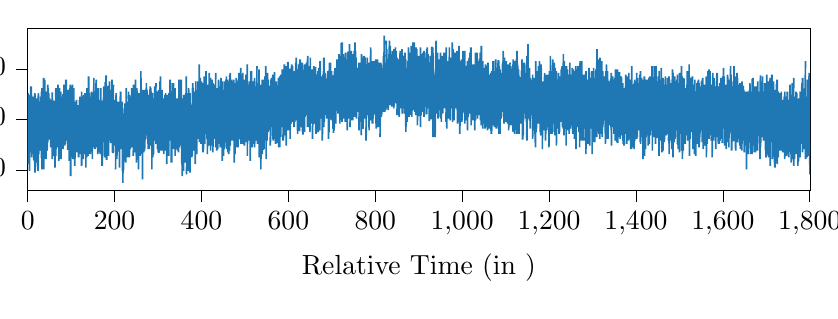
\begin{tikzpicture}[
baseline,
trim axis right,
trim axis left
]

\definecolor{color0}{rgb}{0.12156862745098,0.466666666666667,0.705882352941177}

\begin{axis}[
height=0.3\textwidth,
tick align=outside,
tick pos=left,
width=0.95\textwidth,
x grid style={white!69.0196078431373!black},
xlabel={Relative Time (in \si{\second})},
xmin=0, xmax=1800.934324955,
xtick style={color=black},
y grid style={white!69.0196078431373!black},
ylabel style={align=center},
ylabel={\(\displaystyle P_{cav}\) (in \si{\kilo\watt})},
ymin=5292.05134765, ymax=5356.13497935,
ytick style={color=black},
yticklabel pos=lower
]
\addplot [semithick, color0]
table {%
0 5307.66003
0.599210530002892 5330.416537
1.20014349100529 5328.406565
0.604668883002887 5307.66003
1.20564956500311 5302.3127
1.80059134900512 5319.032053
1.80488658700051 5309.665983
2.40015559599851 5317.693813
2.4044899090004 5307.66003
3.00015635599993 5329.07669
3.60002171800443 5329.746412
3.00477137100097 5325.057549
4.20005537300312 5325.057549
3.60468447900348 5311.672338
4.79933050399995 5326.396994
4.20570347700414 5299.639838
5.40010526600236 5327.736842
4.80554769300215 5312.341256
6.00008943400462 5321.040417
5.40552414500416 5312.341256
6.59969108000223 5329.07669
6.00505207000242 5317.024492
7.14079292699898 5333.097037
6.60490418300469 5306.991514
7.2037514170006 5328.406565
7.80391753400181 5333.097037
7.80614374900324 5309.665983
8.4039020880009 5333.097037
8.40633957600221 5317.024492
9.00389262800309 5329.746412
9.60376314400492 5319.701374
9.0057103920044 5304.985963
9.60589269200136 5309.665983
10.2052340110022 5319.032053
10.206059119002 5315.016932
10.8046210890025 5319.701374
10.8060877989992 5317.024492
11.3100734440013 5329.07669
11.4062680120041 5319.032053
12.0061571590049 5325.727271
12.1100734440042 5308.997064
12.6060552230047 5323.718505
13.2015439009992 5327.736842
12.606648990004 5310.3345
13.2072170710017 5306.322997
13.8019237379995 5327.736842
14.4029025080017 5315.686253
13.8074959950027 5304.317446
14.4082051549995 5304.317446
15.0032442709999 5329.07669
15.0085364330007 5303.649331
15.6036267630043 5327.067119
15.6083816530008 5303.649331
16.2039221470041 5330.416537
16.8078352130033 5329.746412
16.2094185489987 5302.3127
17.4078033469996 5315.016932
16.8103711910007 5298.971723
17.409710179003 5302.3127
18.0093144839993 5321.709738
18.6086201380022 5321.709738
18.0101490230008 5312.341256
19.0790734440016 5313.010175
18.6105129190037 5304.317446
19.2101270810017 5302.980815
19.8063434310025 5317.024492
20.406973615005 5325.727271
19.8118566330013 5313.010175
20.4118007850047 5306.322997
21.0076249350022 5328.406565
21.6079832169999 5325.057549
21.0122718130006 5315.016932
21.6127878430052 5313.010175
22.0820734439985 5323.048782
22.2116834850021 5304.985963
22.6800734440039 5325.057549
23.4088680120039 5324.387826
22.8129082110027 5311.003419
23.4148056030026 5299.639838
24.009061757999 5324.387826
24.6094800819992 5330.416537
24.0146682630002 5299.639838
24.6154409160008 5303.649331
25.2107024350044 5329.746412
25.216149576001 5306.322997
25.8112068140035 5323.718505
25.816120471005 5306.322997
26.411631889001 5325.727271
26.4163148730004 5311.672338
26.9260734440031 5321.709738
27.0156238290001 5311.672338
27.5270734439982 5323.048782
27.6154925480005 5308.997064
28.0830734440024 5323.718505
28.6850734440013 5326.396994
28.2169365770023 5307.66003
29.2860734440037 5327.067119
28.8174149080005 5313.679094
30.0130987900047 5329.07669
29.4175243830032 5315.686253
30.6133290590005 5329.07669
30.0196176030004 5308.997064
31.2148164399987 5325.057549
30.6187859659985 5309.665983
31.2203590339996 5311.672338
31.8150027119991 5331.086662
32.4152249210019 5317.024492
31.8203227470003 5304.985963
32.4211072730031 5304.985963
33.0157443900025 5332.426912
33.0213852540037 5300.307953
33.5320734440029 5330.416537
34.1280734440006 5325.057549
33.6198015180053 5300.307953
34.7310734440034 5325.057549
34.2195266909985 5313.679094
35.3300734440054 5320.371097
34.8208756980021 5305.65448
35.8900734440031 5329.07669
35.4215349689985 5305.65448
36.4880734440012 5336.448465
36.0222553179992 5317.693813
36.620767694003 5300.307953
37.2171987710026 5336.448465
37.2233513860047 5300.307953
37.8182959650003 5329.07669
37.8236907200044 5304.985963
38.4185219400024 5329.07669
38.4238782910033 5304.985963
39.0188724399995 5327.736842
39.0242108509992 5311.672338
39.6194169220034 5335.77834
39.6249113020021 5309.665983
40.2193532640013 5321.709738
40.2249561880017 5309.665983
40.6930734440029 5326.396994
40.8237374000018 5307.66003
41.4110734440037 5326.396994
41.9360734440052 5331.086662
41.4233732180001 5304.317446
42.5390734440007 5327.736842
42.0233759930052 5304.317446
43.094073444001 5325.727271
42.6250020350053 5311.672338
43.6970734440038 5327.067119
43.2249733510034 5313.679094
44.4207369680007 5327.067119
43.825325251004 5317.693813
45.0209981299995 5321.040417
44.4268745220033 5307.66003
45.026682335003 5308.997064
45.6212183969983 5328.406565
45.6275525930032 5313.679094
46.2214838069995 5333.767161
46.2273982510014 5311.003419
46.8223811210046 5332.426912
46.8277771409994 5315.016932
47.4226542219985 5329.07669
48.0231743390032 5330.416537
47.4281039929992 5313.010175
48.623028177004 5330.416537
48.0280022410006 5312.341256
48.6282199690031 5312.341256
49.2234402950053 5322.379461
49.7020734440011 5321.709738
49.2288481659998 5315.016932
49.827638859002 5315.686253
50.3030734440035 5327.067119
50.4272700660003 5314.348013
50.9020734439982 5328.406565
51.0275100889994 5312.341256
51.5020734440041 5323.718505
52.104073444003 5321.709738
51.6290410760048 5312.341256
52.2291319270007 5313.679094
52.7460734440028 5321.709738
52.8283755410012 5308.997064
53.3010734440031 5320.371097
53.4292603130016 5308.997064
54.0250476910005 5325.727271
54.0316643480037 5309.665983
54.6252546780015 5324.387826
55.2257521409992 5327.736842
54.6308417460023 5312.341256
55.8268121830042 5327.736842
55.2315851849999 5313.010175
55.8324019350039 5320.371097
56.4270429829994 5330.416537
56.9460734439999 5330.416537
56.4324164900027 5304.317446
57.0314908299988 5311.672338
57.5460734439985 5327.736842
58.1470734440009 5322.379461
57.6310261590043 5307.66003
58.6334739430022 5314.348013
58.232566769002 5306.322997
59.3470734440052 5317.693813
58.8324083530024 5312.341256
59.4325955169988 5305.65448
60.028749776 5313.679094
60.0340433340025 5307.66003
60.6292060230044 5325.057549
60.6350512979989 5311.003419
61.2296616660024 5325.057549
61.2350940290053 5311.003419
61.8307592839992 5327.067119
62.4310725030009 5327.067119
61.8360820200032 5319.701374
62.4366364960006 5305.65448
62.956073444002 5321.040417
63.034835506005 5300.976068
63.5090734440018 5323.718505
63.6347482240017 5310.3345
64.1510734440017 5323.718505
64.7100734440028 5331.756787
64.2365330540051 5310.3345
64.8369555210011 5305.65448
65.3190734439995 5332.426912
65.4373115679991 5308.328547
65.9110734440037 5321.709738
66.037279850003 5315.016932
66.6328501500029 5331.086662
67.2331783250047 5331.086662
66.6386630179986 5322.379461
67.8335072970003 5330.416537
67.2387709670002 5325.727271
67.8390780090049 5320.371097
68.4338660170033 5329.746412
69.0345331470016 5321.709738
68.440179889003 5318.363134
69.0399408060039 5308.997064
69.634337028001 5333.767161
70.1110734440008 5323.718505
69.6404432400013 5308.997064
70.7120734440032 5321.040417
70.2388546060029 5313.679094
71.3130734439983 5324.387826
70.8388732009989 5316.355172
71.440398358005 5303.649331
71.9110734440037 5324.387826
72.5540734440001 5332.426912
72.0405794640028 5309.665983
73.1160734439982 5332.426912
72.6409073480027 5315.016932
73.8365301750018 5321.709738
73.2411517319997 5315.016932
74.436824825003 5325.057549
73.8428113590053 5312.341256
75.0371292230047 5323.048782
74.4427672829988 5315.686253
75.6375259720007 5329.746412
75.0427994560014 5322.379461
75.6435990919999 5318.363134
76.2386809279997 5331.086662
76.2436047400042 5304.317446
76.8383764270038 5323.048782
76.8446866240047 5304.317446
77.3430734440044 5322.379461
77.4431468900002 5322.379461
77.9210734439985 5326.396994
78.0426521570043 5310.3345
78.5210734440043 5325.057549
78.6440598560002 5313.679094
79.1670734440049 5329.07669
79.2445175270041 5312.341256
79.7690734440039 5329.07669
79.8449740490032 5308.328547
80.3220734440038 5321.709738
80.4447217050038 5308.328547
81.0405712030042 5329.746412
81.6408507710003 5329.746412
81.0460622180035 5313.679094
81.6466415040049 5308.328547
82.2414109710007 5325.057549
82.2466721329984 5312.341256
82.8415584300019 5329.746412
82.847331115001 5309.665983
83.4426179540023 5333.767161
83.4479355580042 5317.693813
84.0422008110036 5333.767161
84.048101846005 5310.3345
84.5270734439982 5317.693813
84.6465194289995 5309.665983
85.1490734440013 5324.387826
85.7720734440009 5329.07669
85.2465458600054 5309.665983
86.3720734439994 5325.727271
85.8480704180038 5311.003419
86.9260734440031 5325.727271
86.4485647760011 5310.3345
87.5710734439999 5335.77834
87.0479952940004 5325.057549
87.649298426004 5324.387826
88.2446972700054 5334.437688
88.8449801410025 5335.77834
88.2505845090054 5326.396994
89.446025160003 5326.396994
88.8511870840011 5313.679094
90.0457654380007 5326.396994
89.4515523630034 5318.363134
90.6462801450034 5324.387826
90.0516401749992 5311.672338
90.6524846629982 5315.016932
91.1350734439984 5323.718505
91.7770734439982 5319.032053
91.2509902640013 5315.016932
92.3810734440049 5331.086662
91.8509157740045 5308.328547
92.4518319999988 5308.328547
92.9370734440017 5331.756787
93.5340734440033 5331.086662
93.0524682360046 5311.672338
93.6528090300053 5310.3345
94.2481619020036 5317.693813
94.2536493200023 5311.672338
94.8484927040045 5321.040417
94.8537923580006 5309.665983
95.4487492769986 5325.727271
96.0490496249986 5325.727271
95.4558504540037 5303.649331
96.0557863360009 5308.328547
96.6490994830019 5330.416537
96.6544949610034 5308.328547
97.2497049390004 5332.426912
97.2555818820038 5317.693813
97.8499588560007 5333.767161
97.8560175150051 5315.016932
98.4510696650032 5333.097037
98.451083164 5297.635494
98.9360734440052 5321.040417
99.0545787779993 5297.635494
99.5360734440037 5328.406565
99.6544674129982 5306.322997
100.143073444 5327.736842
100.739073444005 5330.416537
100.256431300004 5306.322997
100.856372991999 5306.322997
101.382073444001 5319.032053
102.05199647 5322.379461
101.455579052999 5311.003419
102.057386 5312.341256
102.652490697001 5329.07669
102.657574399003 5313.679094
103.252445704005 5333.767161
103.258274737003 5304.985963
103.852877047 5323.048782
103.858465017001 5304.985963
104.453079872001 5321.040417
104.459544998004 5304.317446
105.053542456 5325.057549
105.059250696999 5304.317446
105.654445161999 5332.426912
105.659773247004 5311.672338
106.192073443999 5332.426912
106.258770291999 5311.003419
106.749073444 5324.387826
107.349073443998 5323.718505
106.858804692005 5311.003419
107.458755789004 5304.985963
107.950073444001 5327.067119
108.060142171998 5301.644183
108.551073444003 5324.387826
108.660705225004 5301.644183
109.255663241005 5325.057549
109.856002527005 5315.686253
109.261143376003 5308.328547
109.861321285003 5307.66003
110.456340058001 5323.048782
110.461770735004 5309.665983
111.056629543004 5325.057549
111.657057827004 5325.057549
111.061961763 5311.003419
112.258093584998 5327.736842
111.663506440003 5306.991514
112.858439124 5319.032053
112.263531271004 5306.991514
113.356073444003 5321.709738
112.863793091004 5309.665983
113.959073443999 5321.709738
113.462317411002 5309.665983
114.560073444001 5315.686253
114.062036563999 5306.991514
115.143073444 5325.727271
114.663761344003 5306.991514
115.859702984002 5325.727271
115.263230805998 5307.66003
115.865013310999 5308.997064
116.460008644004 5324.387826
117.060377040005 5322.379461
116.465416128005 5313.679094
117.660798736004 5323.048782
117.065783180005 5304.985963
118.261346633 5323.048782
117.666334402005 5304.985963
118.714073444004 5321.709738
118.261357378004 5307.66003
119.318073444003 5327.736842
118.861813214004 5306.322997
120.011073444002 5327.736842
119.466523996001 5308.997064
120.066438900001 5313.010175
120.570073444003 5329.07669
120.667335966005 5306.991514
121.144073444004 5321.709738
121.267740019 5306.991514
121.771073444004 5321.709738
121.868280668001 5306.322997
122.413073444004 5315.016932
122.463848672 5315.016932
122.969073444001 5325.727271
123.064252279 5306.991514
123.569073444 5325.727271
123.664532134004 5301.644183
124.229073444003 5331.086662
124.264880152004 5301.644183
124.770073444 5325.057549
124.865301967002 5311.672338
125.372073443999 5325.057549
125.465643736999 5311.672338
125.971073444001 5321.040417
126.069935173 5314.348013
126.615073444002 5327.067119
126.669795601003 5317.693813
127.220073444005 5324.387826
127.271690414003 5304.317446
127.723073444002 5319.701374
127.871959741002 5304.317446
128.421073443998 5329.07669
128.467506131004 5306.991514
128.976073443999 5329.746412
129.067685198999 5306.991514
129.625073444004 5318.363134
129.668284113002 5318.363134
130.148073444005 5323.718505
130.268574564005 5308.997064
130.781073443999 5318.363134
130.868692418 5306.322997
131.329073444002 5319.032053
131.468954930002 5315.016932
131.981073444003 5330.416537
132.069282005003 5314.348013
132.626073444 5330.416537
132.670151750004 5314.348013
133.182073444004 5328.406565
133.274423046001 5311.672338
133.782073444003 5325.057549
133.874304814002 5300.976068
134.381073444005 5327.736842
134.475411960004 5310.3345
135.027073443998 5322.379461
135.075728511001 5310.3345
135.583073444002 5329.07669
135.675949534001 5304.985963
136.183073444001 5332.426912
136.276086049002 5304.985963
136.783073443999 5328.406565
136.876503289001 5311.003419
137.382073444001 5324.387826
137.476797341005 5311.003419
137.984073444 5324.387826
138.071931031998 5309.665983
138.585073444003 5330.416537
138.671952666002 5305.65448
139.185073444001 5330.416537
139.272286076004 5308.328547
139.872491728005 5337.118992
139.878671099999 5315.686253
140.472685145003 5337.118992
140.478752530005 5316.355172
141.072895744001 5330.416537
141.078688852002 5311.672338
141.673098161998 5330.416537
141.679055239001 5306.322997
142.273352057004 5319.032053
142.278979338 5306.322997
142.786073444004 5325.057549
142.877791022001 5315.016932
143.280076135001 5323.718505
143.477643505001 5319.032053
143.987073444005 5329.07669
144.077710825004 5306.322997
144.588073444 5323.718505
144.677643037001 5315.686253
145.187073444002 5323.048782
145.279379369 5306.991514
145.788073444004 5327.067119
145.879600988999 5308.328547
146.388073444003 5327.067119
146.479025109998 5306.991514
146.989073444005 5331.086662
147.079999426998 5310.3345
147.589073444004 5328.406565
147.680532478 5311.003419
148.275914768004 5328.406565
148.281134165001 5315.686253
148.876233003 5329.746412
148.882914595 5304.317446
149.476549352999 5329.746412
149.481906524001 5308.328547
150.076604309004 5322.379461
150.082142008003 5317.024492
150.677131935001 5329.746412
150.683679189999 5315.686253
151.277178346005 5330.416537
151.283139491999 5311.003419
151.795073444002 5322.379461
152.395073444 5336.448465
151.881561006005 5315.686253
152.996073444003 5317.024492
152.481575204001 5308.997064
153.596073444001 5329.07669
153.083082499004 5308.997064
154.197073444004 5329.746412
153.683311318004 5311.672338
154.797073444002 5329.07669
154.283781413003 5316.355172
155.479425491001 5329.07669
154.883993515003 5308.328547
156.079912791 5329.746412
155.484735796999 5321.040417
156.680099862002 5331.086662
156.085153812004 5320.371097
157.280513507001 5334.437688
156.685605938001 5320.371097
157.880719635003 5335.77834
157.285967882002 5317.693813
158.481056267003 5324.387826
157.886284366003 5316.355172
159.003073444001 5320.371097
158.486657246001 5316.355172
159.602073444003 5330.416537
159.085420743002 5308.997064
160.216073444004 5326.396994
159.685427421005 5308.997064
160.804073444 5326.396994
160.285912520005 5315.016932
161.406073443999 5323.718505
160.887669456002 5313.010175
161.487500169998 5306.322997
162.082887274999 5332.426912
162.088971782003 5311.003419
162.683127891003 5332.426912
162.688370240001 5311.003419
163.283514891998 5318.363134
163.288768885002 5313.010175
163.883780159005 5327.067119
163.889246929 5323.718505
164.484112470003 5327.067119
164.489527209 5306.991514
165.084498340999 5327.736842
165.089778316004 5306.991514
165.684723273 5327.736842
165.690353495003 5315.686253
166.285063690004 5320.371097
166.291071710002 5315.686253
166.812073444002 5323.048782
166.889891621999 5306.322997
167.412073444 5323.048782
167.490006956999 5307.66003
168.015073444003 5332.426912
168.09013389 5310.3345
168.617073444002 5317.024492
168.692719798004 5307.66003
169.286870831005 5322.379461
169.292152237002 5307.66003
169.887222365003 5327.067119
170.487581746005 5327.067119
169.892532969003 5308.328547
171.087827846 5322.379461
170.492778309002 5306.991514
171.093155325005 5301.644183
171.688248897 5323.718505
172.288547001001 5327.067119
171.693876344005 5301.644183
172.293848918001 5308.997064
172.888804545 5316.355172
172.894426252999 5311.003419
173.416073444001 5322.379461
174.019073444004 5327.736842
173.493567704005 5321.040417
174.093757303999 5316.355172
174.619073444002 5328.406565
174.693349093002 5316.355172
175.216073444004 5333.097037
175.816073444003 5330.416537
175.294839510003 5312.341256
176.424073444003 5328.406565
175.895174896003 5312.341256
176.494467456003 5311.003419
177.090956359003 5326.396994
177.691896909004 5329.07669
177.096242781001 5304.985963
177.696537290001 5306.322997
178.291580771001 5334.437688
178.891736799 5334.437688
178.296705339002 5313.010175
178.897029051004 5315.016932
179.491924351001 5333.767161
179.497356803004 5311.672338
180.092613427005 5337.118992
180.692614767002 5337.118992
180.098852599003 5319.701374
181.238073444001 5327.736842
180.698058915004 5323.718505
181.830073444005 5332.426912
181.297307332003 5304.317446
181.897623353005 5304.317446
182.428073444004 5327.736842
183.031073443999 5329.07669
182.497625231001 5309.665983
183.098884693005 5308.328547
183.632073444001 5329.07669
184.235073444004 5333.097037
183.699181778 5308.328547
184.836073443999 5329.746412
184.299641165999 5317.693813
184.899652092005 5320.371097
185.437073444002 5333.097037
186.095656554004 5333.097037
185.500219476002 5320.371097
186.100870678005 5305.65448
186.695918001999 5325.057549
186.701397763005 5311.672338
187.296392852004 5325.057549
187.896605740003 5330.416537
187.301707365004 5311.672338
188.439073444002 5335.107813
187.902659788 5330.416537
189.037073444 5330.416537
188.501796821001 5312.341256
189.670890819005 5322.379461
189.101515766 5313.679094
190.242073444002 5331.756787
189.700971188999 5313.679094
190.842073444001 5331.086662
190.302733390003 5316.355172
191.499093260005 5331.086662
190.902844451004 5311.003419
191.504326396003 5311.003419
192.098613466005 5329.746412
192.103831058004 5314.348013
192.698758908999 5329.746412
193.299169966005 5328.406565
192.704032364003 5313.010175
193.305323749999 5313.010175
193.900061758999 5335.77834
194.500378069999 5332.426912
193.904636749001 5317.693813
195.099893808001 5333.097037
194.505080391005 5318.363134
195.105276437003 5306.991514
195.700128249999 5325.057549
196.300366020005 5327.736842
195.705404560002 5306.991514
196.305702831 5306.991514
196.900611602003 5327.736842
197.353073443999 5333.767161
196.906940141002 5306.991514
197.957073443999 5327.067119
197.504832203005 5311.003419
198.105361779999 5319.032053
198.557073444004 5326.396994
198.705175872004 5309.665983
199.199073444004 5326.396994
199.307007879004 5309.665983
199.758073444005 5323.048782
199.906039633999 5311.672338
200.355073444 5327.736842
200.956073444002 5321.040417
200.506980896003 5313.010175
201.107096211002 5313.010175
201.702538821002 5321.040417
201.708787493 5319.701374
202.302806420004 5323.718505
202.903058675998 5323.718505
202.308153044003 5300.307953
203.503438004998 5330.416537
202.908527079999 5313.679094
204.103815975999 5329.07669
203.508767068 5311.672338
204.704074699999 5327.067119
204.109207103 5313.679094
205.304444246001 5327.067119
204.709371142999 5314.348013
205.763073444003 5321.709738
205.309746596999 5304.317446
206.362073444005 5321.709738
205.908697453 5307.66003
206.963073444 5313.679094
206.508690248003 5307.66003
207.109420911002 5307.66003
207.564073444002 5321.040417
208.164073444001 5317.693813
207.711017226 5310.3345
208.764073443999 5322.379461
208.310567458 5308.997064
209.507154674 5327.067119
208.910161204003 5313.679094
210.106720324999 5327.067119
209.512581852003 5307.66003
210.112648640003 5307.66003
210.707067625 5320.371097
211.308251428003 5325.057549
210.712374451003 5313.679094
211.313059986001 5300.976068
211.907776143002 5314.348013
212.508232573004 5325.057549
211.913147817002 5313.010175
213.108427918 5329.07669
212.513709980005 5321.040417
213.570073444003 5331.086662
213.114638872001 5318.363134
214.255073444001 5331.086662
213.712511432001 5311.672338
214.814073444002 5323.718505
214.315014871005 5313.679094
214.915324159003 5312.341256
215.414073444001 5323.718505
215.514597068002 5309.665983
215.973073444002 5321.709738
216.115046461004 5308.328547
216.710327790002 5323.718505
216.717171822005 5308.328547
217.311483022 5327.067119
217.316879351005 5309.665983
217.910957372005 5327.067119
217.916662073003 5299.639838
218.511115991001 5317.693813
218.516402542002 5299.639838
219.112481159005 5317.693813
219.117981821 5294.96424
219.712439587005 5319.701374
219.718097466 5299.639838
220.312904617 5319.701374
220.91232974 5311.672338
220.317333257 5299.639838
220.917872585 5306.322997
221.512376756 5317.024492
221.517785182004 5308.997064
222.018073444 5317.024492
222.619073444002 5324.387826
222.117322131999 5308.328547
223.273073444005 5315.686253
222.716604453002 5303.649331
223.823073444 5326.396994
223.316856973004 5303.649331
224.428073444004 5326.396994
223.919257852001 5303.649331
224.518081204005 5309.665983
225.023073444005 5322.379461
225.581073444002 5321.040417
225.119257081999 5317.024492
226.183073444001 5324.387826
225.718580200002 5302.980815
226.822073444004 5332.426912
226.318653091999 5316.355172
227.515532685 5327.067119
226.918917770003 5309.665983
228.114928218005 5327.067119
227.520777634003 5309.665983
228.120421716005 5309.665983
228.715096644002 5313.010175
228.720404801003 5304.985963
229.316384862002 5317.693813
229.915604608002 5318.363134
229.321675753003 5304.985963
230.515887134003 5325.057549
229.922081811004 5307.66003
230.522328265004 5307.66003
231.115971979001 5321.709738
231.589073444004 5325.727271
231.121391715998 5307.66003
232.320503631003 5331.086662
231.720901549001 5315.686253
232.323129825003 5313.679094
232.792073444005 5327.736842
233.428073444004 5327.067119
232.921838341004 5313.679094
233.993073443999 5329.746412
233.522050676002 5304.985963
234.628073444001 5326.396994
234.122379123 5304.985963
234.723479403001 5311.003419
235.319220256002 5326.396994
235.323554622999 5308.328547
235.918974762004 5327.067119
235.924302865002 5308.328547
236.519079205005 5327.067119
237.120396413004 5329.07669
236.525298510001 5319.701374
237.124637271001 5311.672338
237.719691793005 5327.736842
237.725305316999 5311.672338
238.320027993999 5329.07669
238.325376604 5311.003419
238.799073444003 5325.727271
239.399073444001 5332.426912
238.924745215001 5311.003419
239.999073444 5332.426912
239.524841530001 5315.016932
240.600073444002 5320.371097
240.126438093001 5308.997064
240.726342351001 5309.665983
241.237073444005 5323.048782
241.834073443999 5330.416537
241.325995879 5315.686253
242.404073443999 5330.416537
241.926366312 5313.010175
243.121840054002 5329.07669
242.526537415004 5313.679094
243.723160316003 5333.767161
243.128016477 5305.65448
244.323447139999 5321.709738
243.727582967003 5308.997064
244.922657175004 5321.709738
244.328734173003 5307.66003
245.523122760002 5310.3345
244.929020674004 5306.991514
246.123184476004 5330.416537
245.528651355002 5306.991514
246.723329594999 5331.086662
246.129497219001 5320.371097
247.323581346005 5331.086662
246.729583556 5308.997064
247.329013488001 5315.016932
247.924513010999 5335.77834
247.928970705005 5319.032053
248.524569493005 5335.77834
248.529286632998 5318.363134
249.123880163999 5329.746412
249.729164848999 5327.736842
249.129637623999 5311.672338
250.328420278005 5319.701374
249.729931536 5309.665983
250.330041214998 5302.980815
250.930011683005 5332.426912
251.530281965999 5331.086662
251.128656198001 5313.010175
251.728187786 5309.665983
252.128325313999 5331.086662
252.130959996 5313.010175
252.729360005003 5326.396994
253.330490756001 5324.387826
252.731486870005 5313.010175
253.931274022005 5324.387826
253.332017200999 5308.328547
254.531482445003 5313.679094
254.048073443999 5304.317446
254.654073443999 5304.317446
255.130915435999 5317.024492
255.732075582004 5321.709738
255.197073444004 5300.307953
255.851073443999 5325.057549
256.331120011004 5327.067119
256.386073444002 5323.048782
256.932119885001 5330.416537
257.531537993003 5319.701374
257.051073444003 5305.65448
258.131950881005 5323.718505
257.655073444002 5317.693813
258.732673707003 5324.387826
258.257073444001 5319.701374
259.332976500998 5330.416537
258.821073444 5305.65448
259.932992080001 5320.371097
259.456073444002 5308.997064
260.061073444005 5306.322997
260.532121525001 5339.130572
261.132291763002 5323.718505
260.656073443999 5319.701374
261.733324346998 5329.746412
261.222073444005 5315.016932
261.821073444 5316.355172
262.332638190004 5322.379461
262.460073444003 5326.396994
262.933515952005 5330.416537
263.064073444002 5312.341256
263.532814871003 5321.040417
264.133131497001 5331.756787
263.623073444003 5319.032053
264.224073443998 5296.300068
264.733212607003 5320.371097
264.865073444002 5312.341256
265.333622677004 5331.086662
265.933662283998 5318.363134
265.425073443999 5311.672338
266.534171517 5325.727271
266.068073444003 5315.686253
267.133810804 5326.396994
266.664073444001 5308.997064
267.269073444004 5306.991514
267.735037273 5329.746412
268.334870138002 5321.709738
267.830073444005 5319.701374
268.935003223 5331.756787
268.467073444001 5327.067119
269.535482842999 5319.032053
269.068073444003 5307.66003
269.631073444005 5310.3345
270.134753580998 5313.679094
270.734719100001 5321.709738
270.268073444 5313.010175
271.335391035005 5327.736842
270.868073443999 5314.348013
271.433073444001 5324.387826
271.935051918001 5330.416537
271.998341039005 5323.718505
272.535130299999 5330.416537
272.676073444003 5313.679094
273.135481042002 5334.437688
273.736205146 5326.396994
273.235073444004 5320.371097
273.873073444003 5314.348013
274.335438521004 5331.756787
274.936730364003 5330.416537
274.436073444005 5314.348013
275.535752856005 5330.416537
275.072073444004 5312.341256
276.13684608 5327.067119
275.672073444002 5324.387826
276.218073444004 5321.040417
276.737151491005 5328.406565
276.875073444004 5310.3345
277.336438283004 5318.363134
277.937793317004 5329.746412
277.382073444001 5308.328547
278.536370459005 5329.746412
278.038073444004 5313.679094
279.136919755001 5327.067119
278.676073444003 5315.016932
279.241073444005 5324.387826
279.737328688003 5329.746412
280.337585934001 5312.341256
279.876073444 5308.328547
280.937997781002 5327.736842
280.477073444003 5309.665983
281.537590209002 5319.032053
281.041073444001 5312.341256
281.675073443999 5331.756787
282.138263594003 5333.097037
282.182073444004 5309.665983
282.737644184002 5327.067119
282.846073444001 5323.048782
283.337606907 5332.426912
283.447073444004 5318.363134
283.937758826003 5326.396994
283.985073444004 5315.016932
284.539445854003 5331.086662
284.586073443999 5315.686253
285.138281983003 5321.709738
285.240073444002 5316.355172
285.739569853999 5326.396994
285.784073444003 5300.307953
286.339742855002 5326.396994
286.386073444002 5311.672338
286.938549012004 5327.736842
286.985073444004 5325.057549
287.539095493004 5330.416537
287.586073443999 5312.341256
288.138659715005 5318.363134
288.184073444005 5304.985963
288.739785127 5313.010175
288.856073444003 5311.003419
289.339666979002 5318.363134
289.487073444005 5306.322997
289.939785092 5323.718505
290.058073444001 5316.355172
290.539820837999 5323.718505
290.660073444 5313.679094
291.139419505998 5326.396994
291.259073444002 5321.709738
291.739920805005 5328.406565
291.859073444 5316.355172
292.339587441005 5333.097037
292.940086979004 5327.736842
292.487073444005 5315.016932
292.992073444002 5323.048782
293.539530644004 5328.406565
294.139540703 5329.07669
293.688073443998 5311.672338
294.295073444002 5319.701374
294.739657115002 5329.07669
295.339735157002 5334.437688
294.793073444001 5329.746412
295.467073444001 5310.3345
295.940430786999 5331.086662
296.541100728005 5329.746412
296.094073444001 5319.032053
297.139854304005 5330.416537
296.734427919 5322.379461
297.740271192 5321.040417
297.296073443998 5314.348013
297.895073444 5318.363134
298.350073444002 5326.396994
298.939906625004 5331.086662
298.474073443998 5308.328547
299.540036004 5324.387826
299.074073444004 5311.003419
299.673073443999 5313.010175
300.140629762005 5329.746412
300.193073444003 5306.991514
300.740020734003 5315.686253
301.340766257003 5331.756787
300.796073443998 5312.341256
301.940952271005 5327.067119
301.395073444 5306.991514
301.996073444003 5306.991514
302.540515499 5329.07669
302.583073444002 5306.991514
303.141276337003 5313.679094
303.741885619005 5316.355172
303.198073444 5308.997064
304.341930577 5335.107813
303.882073444001 5309.665983
304.942209754001 5329.07669
304.399073444001 5308.997064
304.984073444 5307.66003
305.541354165005 5337.118992
306.142176551999 5317.693813
305.599073443998 5312.341256
306.741990763003 5330.416537
306.199073444004 5320.371097
306.842073444001 5319.701374
307.344407772005 5322.379461
307.388073444003 5320.371097
307.94334826 5331.086662
308.543102834003 5329.746412
308.047073444002 5317.693813
309.142899842001 5331.756787
308.646073444004 5307.66003
309.202073444001 5311.003419
309.742787977004 5315.686253
310.343811289 5320.371097
309.794073444005 5313.010175
310.944213788003 5323.718505
310.404073443999 5319.032053
311.543748835 5323.048782
311.008073444005 5313.679094
312.144680885001 5325.727271
311.638073444003 5311.672338
312.745089976001 5321.040417
312.196073444 5314.348013
313.345256339999 5328.406565
312.795073444002 5306.991514
313.945650498004 5327.067119
313.395073444 5306.322997
314.544918671003 5316.355172
313.996073444003 5311.672338
315.145409853001 5323.048782
314.597073444005 5314.348013
315.746817125 5329.746412
315.199073444004 5317.693813
316.346574607 5326.396994
315.844073444001 5317.024492
316.946146348004 5328.406565
316.457073443999 5313.010175
317.546836845002 5330.416537
316.999611940999 5307.66003
318.147059506002 5323.048782
317.611073444001 5313.010175
318.747390675002 5329.746412
318.246073444003 5315.016932
319.347915040998 5327.067119
318.859073444 5317.024492
319.403073444002 5313.010175
319.948000276003 5320.371097
320.547867497 5321.709738
320.046073443998 5302.3127
321.148602601002 5325.727271
320.648073444005 5313.679094
321.748926208005 5325.727271
321.262073443999 5311.003419
322.349376572005 5329.746412
321.804073444 5314.348013
322.424073444003 5318.363134
322.949296636005 5323.718505
323.022073444001 5307.66003
323.549507677999 5329.07669
323.609073444 5313.679094
324.149694723004 5323.048782
324.223073444002 5311.672338
324.750612510004 5321.040417
324.812073444002 5305.65448
325.350695305002 5330.416537
325.466073444004 5313.679094
325.950479220999 5325.057549
326.550821517005 5327.067119
326.013073444003 5313.679094
327.151079952004 5322.379461
326.670073444002 5315.686253
327.751641616 5335.77834
327.230073444 5317.024492
328.352112288005 5335.77834
327.770907466998 5317.693813
328.430073444004 5311.672338
328.952185599002 5329.07669
329.015073444003 5317.693813
329.551827373005 5319.701374
330.152838881004 5325.057549
329.675073443999 5315.016932
330.753152060999 5328.406565
330.262073443999 5302.980815
331.353224731 5323.718505
330.858073444004 5321.040417
331.952774096004 5331.086662
331.484073444 5302.980815
332.552736030004 5325.727271
332.043073444001 5314.348013
333.153080308999 5334.437688
332.662073444 5318.363134
333.753414327002 5332.426912
333.263073444003 5309.665983
334.353939660999 5327.736842
333.820073444003 5311.672338
334.953910194999 5330.416537
334.440073443999 5318.363134
335.553874509002 5334.437688
335.088073444 5309.665983
336.154403831002 5328.406565
335.667073444005 5313.010175
336.754917659004 5328.406565
336.229073444003 5308.328547
337.354237865999 5323.718505
336.888073444003 5313.010175
337.955376897 5322.379461
337.468073444004 5316.355172
338.555038658 5320.371097
338.043073444001 5315.686253
339.154763908002 5332.426912
338.689073444002 5313.010175
339.755379603004 5313.679094
339.291073444001 5305.65448
340.355554624002 5325.057549
339.847073444005 5317.693813
340.955462506005 5324.387826
340.470073444005 5311.003419
341.555841351001 5320.371097
341.047073444002 5314.348013
342.155886706001 5327.067119
341.647073444001 5313.679094
342.756024887 5328.406565
342.230073444 5313.010175
343.356880922998 5318.363134
342.893073444 5308.997064
343.496073444003 5308.328547
343.956679278999 5319.701374
344.556497180005 5328.406565
344.049073444003 5323.718505
345.157006448004 5317.024492
344.679073444 5307.66003
345.256073444005 5313.010175
345.757233830998 5327.736842
345.954531898999 5313.010175
346.358201353003 5322.379461
346.957430372 5323.718505
346.438073443998 5311.672338
347.557388100002 5315.016932
347.095073444005 5306.991514
348.157830206001 5335.77834
347.638073444003 5311.003419
348.235073444004 5308.997064
348.757812929005 5335.77834
348.850073444002 5311.672338
349.358038167004 5316.355172
349.454073444002 5317.693813
349.957402541004 5327.736842
350.054073444 5311.672338
350.557541344999 5327.736842
350.654073443999 5321.709738
351.158324921002 5331.086662
351.758886996999 5323.718505
351.243073443999 5315.686253
352.358205582001 5331.756787
351.855073444 5315.686253
352.958315511001 5326.396994
352.404073443999 5309.665983
353.559002510003 5335.77834
353.004073444004 5312.341256
354.158444893001 5319.032053
353.700073444001 5309.665983
354.758815226 5307.66003
354.256073444005 5302.980815
355.358889571005 5323.048782
354.859073444 5315.016932
355.552903087999 5297.635494
355.958612882001 5315.016932
356.006073444005 5303.649331
356.558635324 5315.686253
356.692073443999 5323.718505
357.159412330999 5328.406565
357.241073444005 5313.679094
357.759659221003 5328.406565
357.808073444001 5315.686253
358.359986486001 5327.067119
358.460073444003 5299.639838
358.959957481005 5329.746412
359.009073444002 5308.997064
359.559590833 5319.032053
359.651073444002 5306.322997
360.160285671001 5317.024492
360.295073444002 5313.679094
360.760243563003 5323.048782
361.360616256003 5311.672338
360.897073444001 5309.665983
361.960487646 5325.057549
361.558695856002 5311.672338
362.560597674004 5329.746412
362.109073444 5316.355172
363.161036030004 5320.371097
362.662073444 5302.980815
363.760991376002 5330.416537
363.244073444002 5302.980815
364.360334791003 5329.07669
363.867073444002 5317.024492
364.961247257001 5337.118992
364.503073444001 5312.341256
365.560947513004 5327.736842
365.059073444005 5321.040417
366.161487039004 5311.672338
365.615073444002 5298.303608
366.761724329001 5325.057549
366.267073444003 5308.997064
367.362007618001 5328.406565
366.868073443999 5321.709738
367.962220746005 5330.416537
367.466073444004 5308.997064
368.561281890004 5327.067119
368.112073444005 5313.679094
368.664073444001 5305.65448
369.162383688003 5317.693813
369.244073444002 5313.679094
369.762346077005 5325.727271
369.865073444002 5299.639838
370.361663053001 5332.426912
370.468073444004 5315.686253
370.962461023002 5331.756787
371.014073443999 5304.985963
371.562665739002 5319.032053
371.666073444001 5311.003419
372.162557117001 5325.727271
372.220073444005 5306.991514
372.762538536001 5322.379461
372.819073444 5306.991514
373.362935516001 5315.016932
373.415073444005 5298.971723
373.962938110999 5330.416537
374.071073444 5310.3345
374.562901636004 5326.396994
374.671073443998 5304.985963
375.162745112 5324.387826
375.216073444004 5313.679094
375.763101461001 5323.718505
375.816073444003 5311.003419
376.363087350001 5322.379461
376.515073444003 5307.66003
376.963142355999 5315.686253
377.071073444 5318.363134
377.563147387998 5323.048782
377.675073443999 5304.985963
378.163273857004 5318.363134
378.252073444004 5316.355172
378.763220509005 5322.379461
378.876073444 5305.65448
379.363268820001 5332.426912
379.519073444004 5311.003419
379.963416359999 5334.437688
380.562781076005 5331.086662
380.023073444005 5308.328547
381.163400598001 5327.067119
380.724073443998 5310.3345
381.763729361999 5321.709738
381.276073444002 5315.686253
382.363669488004 5330.416537
381.878073444001 5312.341256
382.963747597001 5325.727271
382.479073444003 5317.693813
383.563763835999 5321.040417
383.024073444001 5307.66003
384.163651178998 5331.086662
383.723073444002 5310.3345
384.764003845004 5331.086662
384.229073444003 5311.003419
385.364160982004 5321.709738
384.883073444005 5314.348013
385.964200977003 5325.727271
385.530073444002 5302.3127
386.563793214998 5329.746412
386.085073444003 5317.024492
387.164370589002 5335.107813
386.687073444002 5310.3345
387.764835314003 5323.718505
387.289073444001 5309.665983
388.364390808005 5319.701374
387.888073444003 5317.693813
388.964528665005 5323.048782
388.485073444004 5313.010175
389.565108077004 5327.067119
389.129359295002 5306.322997
390.165306473005 5329.07669
389.731073444003 5315.016932
390.7643685 5331.756787
390.276073444002 5314.348013
391.364740088 5329.07669
390.887073443999 5324.387826
391.965203947002 5335.107813
391.532073444003 5324.387826
392.565228217005 5326.396994
392.088073444 5321.040417
392.689073444002 5317.693813
393.165292123005 5330.416537
393.290073444005 5321.709738
393.765535067003 5325.057549
393.892073444003 5312.341256
394.366183038001 5329.746412
394.435073444001 5314.348013
394.966242130002 5341.813081
395.136073444002 5320.371097
395.566475198 5331.756787
395.639073443999 5311.003419
396.167205543999 5335.107813
396.257073444001 5313.679094
396.767830279001 5321.040417
396.835073444003 5319.701374
397.367484284005 5336.448465
397.492073444002 5317.024492
397.967604506004 5324.387826
398.092073444001 5318.363134
398.567572616004 5332.426912
398.694073444 5310.3345
399.168219496001 5327.736842
399.295073444002 5311.003419
399.768925281001 5332.426912
399.895073444 5316.355172
400.369047483 5335.107813
400.496073444003 5317.693813
400.968816262 5331.756787
401.096073444001 5315.016932
401.568891272 5323.718505
401.695073444003 5311.003419
402.169052299003 5316.355172
402.295073444002 5311.003419
402.770304631005 5328.406565
402.896073444004 5307.66003
403.370708212002 5318.363134
403.495073443999 5306.991514
403.970796874004 5334.437688
404.096073444001 5307.66003
404.570300468004 5323.718505
404.700073444001 5308.328547
405.171203269005 5326.396994
405.265073444003 5310.3345
405.771439092001 5334.437688
405.903073444002 5313.010175
406.371764285999 5337.118992
406.503073444001 5314.348013
406.972049344004 5321.709738
407.103073443999 5312.341256
407.572757362002 5327.736842
407.703073444005 5310.3345
408.172160003 5331.086662
408.304073444 5315.686253
408.773236150999 5329.746412
408.906073443999 5317.693813
409.373673686001 5326.396994
409.506073444005 5320.371097
409.973936362003 5329.07669
410.106073444003 5314.348013
410.572967395005 5339.130572
410.711073443999 5315.686253
411.173610903003 5330.416537
411.271073444004 5315.686253
411.773471938002 5327.067119
411.817073443999 5316.355172
412.372814981005 5322.379461
412.417073444005 5312.341256
412.980894660999 5318.363134
413.108073444004 5319.701374
413.573008905005 5333.767161
413.622073443999 5306.322997
414.173156239005 5327.067119
414.217073444001 5317.024492
414.773460028999 5330.416537
414.826073444005 5311.003419
415.372781894002 5331.756787
415.424073444003 5310.3345
415.972887447999 5333.767161
416.023073444005 5311.003419
416.572882859 5333.767161
416.620073443999 5309.665983
417.210419708004 5328.406565
417.252073444004 5320.371097
417.773503272001 5338.460045
417.823073444 5320.371097
418.372881759999 5335.107813
418.972779610005 5322.379461
418.428073444004 5312.341256
419.616073444005 5335.107813
419.027073443998 5321.040417
420.172750087004 5335.107813
419.767406853003 5329.746412
420.817073443999 5336.448465
420.225073444002 5315.686253
421.372560053998 5321.040417
420.967640991999 5307.66003
421.973687837999 5328.406565
421.427073444 5313.010175
422.573005080005 5323.718505
422.027073443998 5314.348013
423.217073444001 5333.767161
422.631073444005 5315.686253
423.772291088004 5333.767161
423.280073444002 5314.348013
424.372581118005 5335.77834
423.835073444003 5323.718505
424.972338236999 5329.746412
424.566771853002 5313.679094
425.619073444002 5332.426912
425.030073444002 5309.665983
426.172814893005 5327.736842
425.766789310001 5315.016932
426.772305929 5334.437688
426.231073444003 5306.991514
427.399756162005 5329.07669
426.832073443999 5311.672338
427.972165251005 5329.07669
427.440073443999 5320.371097
428.573109050005 5325.057549
428.036073444004 5317.693813
429.171603670999 5327.067119
428.639073443999 5319.701374
429.772260160003 5332.426912
429.238073444001 5325.727271
430.372056551001 5326.396994
429.839073444004 5317.693813
430.972316251005 5333.767161
430.443073444003 5315.686253
431.572062769999 5320.371097
431.024073444001 5312.341256
432.172163000003 5328.406565
431.625073444004 5317.693813
432.771859474 5338.460045
432.243073443999 5325.057549
433.37262953 5327.067119
432.842073444001 5308.997064
433.427073444 5319.701374
433.971995418004 5323.718505
434.047073444002 5317.024492
434.572068002002 5328.406565
434.646073444004 5321.709738
435.172035740005 5329.746412
435.246073444003 5307.66003
435.771842932001 5326.396994
435.831073444002 5312.341256
436.371835479003 5332.426912
436.432073444004 5317.024492
436.972332299003 5327.736842
437.047073444002 5313.679094
437.572187185004 5331.086662
437.650073444005 5308.328547
438.172484727002 5317.024492
438.234073444 5316.355172
438.772558281002 5327.067119
438.836073443999 5315.016932
439.371772261999 5335.77834
439.435073444001 5310.3345
439.972161669 5335.107813
440.051073444003 5315.016932
440.571419347005 5333.097037
440.651073444002 5315.686253
441.171399611005 5323.048782
441.236073444001 5310.3345
441.771950886003 5328.406565
441.837073444003 5315.016932
442.371325124004 5331.756787
442.439073444002 5317.693813
442.971393275002 5327.067119
443.051073444003 5308.997064
443.571224218002 5326.396994
443.655073444002 5327.067119
444.171288234 5332.426912
444.252073444004 5317.693813
444.771195314999 5336.448465
444.855073444 5313.010175
445.371440966999 5321.040417
445.443073444003 5313.679094
445.970635293001 5327.067119
446.042073444005 5314.348013
446.570399465003 5326.396994
446.655073444002 5322.379461
447.170244676003 5335.107813
447.244073444002 5311.003419
447.770586046005 5321.040417
447.858073444004 5303.649331
448.370163222004 5330.416537
448.454073444002 5317.024492
448.970508634004 5329.07669
449.058073444001 5307.66003
449.569955076004 5331.086662
449.655073444002 5313.010175
450.169652121003 5328.406565
450.251073444 5310.3345
450.770490392002 5323.718505
450.858073444004 5305.65448
451.369628894005 5331.756787
451.458073444002 5315.686253
451.969801753003 5331.756787
452.054073444 5308.328547
452.569540130004 5335.107813
452.651073444002 5319.032053
453.169481443001 5330.416537
453.258073444005 5311.003419
453.769648308 5323.718505
453.858073444004 5317.693813
454.369748595003 5333.767161
454.458073444002 5322.379461
454.970202597004 5327.736842
455.054073444 5317.693813
455.569445646004 5331.086662
455.658073443999 5321.709738
456.170510655 5335.77834
456.262073443999 5313.010175
456.770684360999 5317.024492
456.866073444005 5308.997064
457.370572858999 5337.118992
457.455073444005 5324.387826
457.970676244004 5335.107813
458.062073444002 5308.328547
458.570204050004 5330.416537
458.666073444001 5311.003419
459.170720524999 5332.426912
459.239073444005 5323.718505
459.769907318005 5335.77834
459.866073444005 5324.387826
460.370468708999 5328.406565
460.459073443999 5317.024492
460.970479624004 5335.107813
461.067073443999 5306.991514
461.571101639005 5331.086662
461.661073444004 5317.024492
462.235073444004 5329.07669
462.368791141998 5322.379461
462.771408689005 5331.756787
462.866073444005 5306.322997
463.370891514001 5330.416537
463.467073444001 5313.679094
463.971092393003 5333.097037
464.075073444001 5322.379461
464.570330697999 5335.107813
464.670073444002 5307.66003
465.170832283999 5337.789518
465.271073444004 5325.057549
465.770940925999 5336.448465
465.873073444003 5312.341256
466.370971927005 5338.460045
466.449004362999 5309.665983
466.970912936005 5319.032053
467.075073444001 5323.048782
467.570806071999 5330.416537
467.675073443999 5315.686253
468.180358329999 5334.437688
468.278073444002 5314.348013
468.770199307 5325.057549
468.878073444001 5329.746412
469.370834658002 5335.77834
469.488073444001 5325.057549
469.969879802004 5335.107813
470.082073443999 5319.701374
470.569712707998 5327.736842
470.679073444 5311.672338
471.170776965999 5312.341256
471.283073443999 5315.686253
471.770393522005 5328.406565
471.888073444003 5321.709738
472.370003573 5333.097037
472.478073443999 5313.679094
472.969516322002 5331.756787
473.083073444002 5313.010175
473.569268038002 5319.701374
473.679073444 5329.07669
474.235073444004 5335.77834
474.287073444 5318.363134
474.769068665999 5325.727271
474.897073444001 5315.686253
475.368718064004 5326.396994
475.491073444005 5302.980815
475.968662008003 5327.736842
476.091073444004 5319.701374
476.568491303005 5333.767161
476.692073443999 5313.010175
477.168291212001 5334.437688
477.294073444005 5306.322997
477.768257651005 5325.057549
477.896073444004 5310.3345
478.368111948002 5323.718505
478.490073444002 5311.672338
478.967858595999 5330.416537
479.082073443999 5317.693813
479.567837210001 5329.07669
479.696073444 5308.997064
480.167583220005 5336.448465
480.275073444005 5308.997064
480.767558140004 5329.746412
480.895073444 5313.679094
481.367335802999 5319.032053
481.499073444 5321.040417
481.967602868004 5335.107813
482.100073444002 5317.024492
482.567620016998 5325.727271
482.761946416998 5314.348013
483.167296174004 5332.426912
483.300073443999 5319.032053
483.767903843 5327.067119
483.961941589005 5308.997064
484.367516286999 5331.756787
484.500073444004 5318.363134
484.966628836999 5335.77834
485.088073444 5311.672338
485.566699170005 5322.379461
485.690073443999 5327.736842
486.209073443999 5338.460045
486.264073443999 5321.040417
486.767040938001 5335.107813
486.966199711002 5321.040417
487.409073444003 5328.406565
487.566327345005 5312.341256
488.009073444002 5331.086662
488.166231504001 5315.686253
488.616073444005 5337.118992
488.766044021999 5325.057549
489.210073444003 5337.118992
489.283073443999 5313.010175
489.767836255 5329.07669
489.907073444003 5314.348013
490.413073444004 5340.471626
490.565969666 5315.016932
490.966991391004 5326.396994
491.100073444002 5310.3345
491.615073444002 5337.118992
491.766138332001 5327.067119
492.167069326002 5337.118992
492.281073443999 5317.693813
492.768057736001 5330.416537
492.903073444002 5321.040417
493.366744627005 5324.387826
493.512073443999 5317.693813
494.019073444004 5333.767161
494.165825945005 5317.693813
494.617073444002 5330.416537
495.243073443999 5338.460045
494.765894256001 5320.371097
495.818073444003 5330.416537
495.366054532999 5310.3345
496.420073444002 5329.07669
495.965217978999 5317.693813
497.010073443998 5331.756787
496.566029778005 5314.348013
497.567490804002 5333.097037
497.165963631 5314.348013
498.219073444001 5335.77834
497.718073444004 5323.718505
498.817073443999 5335.77834
498.366129531001 5309.665983
499.414073444001 5330.416537
498.966063119005 5309.665983
500.016073444 5325.727271
499.565695069999 5317.024492
500.615073444002 5327.067119
500.162314916 5317.693813
501.242073444002 5327.067119
500.761734854001 5318.363134
501.817073443999 5333.097037
501.362531463004 5321.709738
502.423073443999 5337.789518
501.962027624002 5327.067119
503.023073444005 5337.789518
502.561991864 5329.07669
503.620073443999 5336.448465
503.162253720002 5311.672338
504.220073444005 5336.448465
503.762496064002 5311.003419
504.820073444003 5333.767161
504.362489726002 5316.355172
505.422073444002 5341.813081
504.962486967001 5316.355172
506.025073444005 5319.701374
505.563376805003 5305.65448
506.627073444004 5332.426912
506.065941951005 5315.686253
507.253073444001 5332.426912
506.763564788998 5317.693813
507.824073444004 5328.406565
507.362610738004 5315.686253
508.428073444004 5333.767161
507.962611923002 5317.693813
509.025073444005 5330.416537
508.562372307999 5319.032053
509.624073444 5333.767161
509.162401089001 5311.672338
510.236073444001 5335.107813
509.762434384 5321.040417
510.832073443999 5321.040417
510.362493380002 5315.016932
511.438073443998 5315.686253
510.962418689 5312.341256
512.028073444002 5332.426912
511.562277650999 5312.341256
512.629073444004 5328.406565
512.162377318004 5303.649331
513.229073444003 5339.130572
512.762370740005 5311.672338
513.834073443999 5327.736842
513.278073444002 5311.672338
514.433073444001 5339.130572
513.962491607002 5319.032053
515.034073444003 5339.130572
514.562621896002 5313.679094
515.637073443999 5335.107813
515.162476477999 5313.679094
516.255073444001 5335.107813
515.762680662003 5325.057549
516.835073444003 5331.756787
516.363410196005 5313.010175
517.439073444002 5327.736842
516.962713313005 5308.997064
518.041073444001 5331.086662
517.562439663001 5311.672338
518.640073444003 5327.736842
518.162617893002 5311.672338
519.241073444005 5331.086662
518.762565265002 5311.672338
519.768831491005 5335.107813
519.362607276998 5318.363134
520.442073443999 5331.086662
519.882073444001 5315.686253
520.968137871001 5330.416537
520.562506388 5315.686253
521.630073444001 5331.086662
521.088073444 5310.3345
522.262073443999 5336.448465
521.762691479998 5315.686253
522.768311170999 5333.097037
522.362571515005 5308.997064
523.447073444004 5331.086662
522.891073444 5315.016932
523.967838338998 5325.057549
523.562507032002 5311.672338
524.638073444003 5329.746412
524.091073444004 5312.341256
525.167573065999 5329.07669
524.762278786999 5315.016932
525.834073443999 5332.426912
525.314073444002 5316.355172
526.398073444005 5332.426912
525.962326596004 5314.348013
526.967576813004 5323.718505
526.540073444005 5311.672338
527.637073443999 5341.142555
527.136073444002 5317.024492
528.167253582003 5325.057549
527.762044144001 5315.686253
528.767877089005 5330.416537
528.291073444001 5323.048782
528.896073444004 5310.3345
529.367662540004 5331.086662
529.967014056005 5334.437688
529.496073444003 5327.067119
530.096073444001 5312.341256
530.566788135999 5325.727271
530.741073444005 5311.003419
531.243073443999 5326.396994
531.362034718004 5319.032053
531.767469404003 5323.718505
532.461073443999 5339.801501
531.897073444001 5317.693813
532.560953284999 5312.341256
532.967225105 5332.426912
533.095073444005 5304.985963
533.642073444003 5322.379461
534.252073444004 5332.426912
533.765917315999 5315.686253
534.365544061002 5313.679094
534.766439065002 5332.426912
535.366743269005 5332.426912
534.898073444005 5317.024492
536.048073443999 5329.746412
535.497073443999 5319.032053
536.5656074 5333.767161
536.164982400005 5321.040417
536.701073444005 5300.307953
537.263073444003 5319.032053
537.363979986003 5305.65448
537.848073444002 5321.709738
538.365647448001 5329.746412
537.963482151004 5321.709738
538.966308089002 5321.709738
538.502073444004 5313.010175
539.650073444005 5335.77834
539.101073443999 5321.040417
539.722255518005 5306.322997
540.207073443999 5329.07669
540.851073443999 5315.686253
540.339073444004 5313.679094
540.963910292005 5315.016932
541.452073444001 5335.77834
542.030793875005 5325.727271
541.563966547001 5308.328547
542.163914955003 5308.328547
542.565386360002 5327.067119
542.704073444002 5310.3345
543.165877766005 5324.387826
543.813073443998 5335.107813
543.304073444 5315.686253
544.459073443999 5335.77834
543.963983788002 5308.328547
544.563165306005 5320.371097
545.013073444003 5335.77834
545.163925581001 5315.686253
545.655073444002 5323.718505
545.763496596999 5321.040417
546.255073444001 5337.118992
546.365028084001 5321.709738
546.808073444001 5327.736842
546.965168750001 5317.024492
547.412073444 5329.07669
547.565268056998 5321.709738
548.054073444 5341.142555
548.165759251999 5319.032053
548.616073444005 5321.709738
548.766158275001 5304.317446
549.265073444003 5325.057549
549.365593684 5325.057549
549.767027144 5332.426912
550.411073444004 5333.097037
549.911073444004 5321.709738
550.967658948 5333.097037
550.566044480998 5325.727271
551.567377300998 5331.086662
551.110073444004 5311.672338
552.284073444003 5338.460045
551.712073444003 5318.363134
552.361422024005 5319.032053
552.819073444 5335.77834
552.961598460002 5315.016932
553.419073444005 5335.77834
553.561821742005 5320.371097
554.018073444 5329.07669
554.162290491004 5323.718505
554.631073444005 5331.086662
554.761966235004 5325.727271
555.270073444 5333.097037
555.362174522001 5318.363134
555.767554329002 5333.097037
555.962370734 5315.686253
556.462073444003 5328.406565
556.562463911003 5318.363134
557.067073443999 5333.097037
557.624073444 5333.097037
557.16260612 5319.032053
557.763008708003 5321.040417
558.233073444004 5327.736842
558.866073444005 5321.040417
558.326073444005 5309.665983
558.967512798001 5312.341256
559.425073443999 5335.77834
559.567679788001 5322.379461
560.029073443999 5335.77834
560.168485266004 5323.718505
560.670073444002 5331.756787
561.271073444004 5336.448465
560.769403978004 5319.701374
561.828073444005 5329.746412
561.369056987001 5319.032053
562.439073444002 5324.387826
561.968553724 5321.040417
562.570002458 5321.040417
563.030073444002 5331.086662
563.671073443998 5331.756787
563.164865529005 5317.024492
564.252073444004 5337.789518
563.765179186004 5317.693813
564.365410090999 5312.341256
564.771039418003 5337.789518
565.479073444003 5333.767161
564.966081936 5311.672338
566.044073444005 5335.107813
565.566271650001 5311.672338
566.166381802999 5325.057549
566.634073444002 5335.107813
567.172276249999 5327.736842
566.766693730999 5320.371097
567.315073443999 5316.355172
567.832073443999 5338.460045
568.431073444001 5338.460045
567.971658677001 5319.701374
568.571175016004 5319.032053
569.075073444001 5329.07669
569.675073443999 5327.067119
569.172656953 5315.686253
570.233073444004 5331.756787
569.772991764003 5314.348013
570.373060786005 5310.3345
570.878601021999 5331.756787
571.438073443998 5329.07669
570.972712588999 5310.3345
571.568627761 5314.348013
572.035073444 5335.107813
572.638073444003 5324.387826
572.168708675999 5313.010175
573.240073444002 5323.718505
572.769280660999 5311.003419
573.836073443999 5323.718505
573.369034401003 5315.016932
573.969336583999 5315.686253
574.417073444005 5322.379461
575.018073444 5333.097037
574.569369851 5315.686253
575.636073444002 5333.097037
575.169446063999 5311.003419
575.769595569 5311.003419
576.292073444005 5329.07669
576.369653667003 5315.016932
576.819073444 5333.097037
577.420073444002 5336.448465
576.969694981999 5317.693813
578.080073444005 5317.693813
577.570351306 5308.997064
578.684073444005 5332.426912
578.169708332003 5308.997064
578.769951906004 5310.3345
579.262073443999 5333.767161
579.370082302004 5308.997064
579.840073444 5337.118992
580.440073443999 5321.040417
579.970083294 5308.997064
581.024073444001 5323.048782
580.570055319004 5314.348013
581.170084251004 5317.024492
581.687073444002 5326.396994
581.770262033999 5322.379461
582.240073444002 5337.789518
582.348073444002 5313.010175
582.839073444004 5337.789518
583.486073444001 5335.107813
582.970339464002 5322.379461
583.570270207005 5322.379461
584.044073444005 5331.086662
584.675073443999 5335.107813
584.170961984004 5319.701374
585.249073444 5337.789518
584.770332717002 5317.024492
585.848073444002 5339.801501
585.370251060005 5323.048782
585.970844732001 5319.701374
586.436073444005 5331.756787
587.086073443999 5333.767161
586.570211022001 5321.709738
587.647073444001 5335.77834
587.170152268001 5320.371097
588.249073444 5331.086662
587.770124704999 5311.672338
588.836073443999 5333.767161
588.369940533004 5311.672338
588.969946138001 5314.348013
589.479073444003 5333.767161
590.037073444 5323.048782
589.569953225 5314.348013
590.694073444 5341.813081
590.169699545004 5318.363134
591.300073443999 5341.813081
590.769510185004 5325.057549
591.369499086999 5319.032053
591.837073444003 5335.107813
591.969230676004 5319.701374
592.500073444004 5335.107813
592.569019927003 5313.679094
593.057073444004 5322.379461
593.168939431998 5319.701374
593.637073443999 5337.789518
593.768485863999 5321.709738
594.260073443998 5337.789518
594.368466940999 5313.679094
594.838073444 5335.107813
595.504073444004 5341.142555
594.968236861001 5309.665983
596.103073443999 5341.142555
595.572586428003 5319.032053
596.703073444005 5339.801501
596.172696567002 5321.709738
597.304073444 5327.736842
596.77242406 5320.371097
597.839073444004 5337.118992
597.372094955004 5321.709738
597.970629029005 5321.709738
598.509073444002 5342.48401
599.109073444 5342.48401
598.570412013003 5317.693813
599.639073443999 5337.789518
599.170661003001 5318.363134
599.770805968001 5315.686253
600.311073444005 5329.07669
600.366305939999 5315.686253
600.841073444004 5333.767161
601.466073444004 5332.426912
600.970791883999 5317.693813
601.565903697003 5331.756787
602.066073444003 5339.801501
602.639073443999 5339.801501
602.165795961002 5316.355172
603.312073444002 5339.801501
602.765712209999 5316.355172
603.871073444003 5336.448465
603.343073444004 5324.387826
604.419073444005 5334.437688
603.966442848003 5312.341256
605.020073444 5334.437688
604.565474294999 5323.048782
605.616073444005 5333.767161
605.165409282999 5320.371097
606.271073444004 5335.107813
605.765467461999 5331.756787
606.365354571004 5318.363134
606.844073444001 5335.107813
607.470073444005 5341.813081
606.965391512 5323.048782
608.075073444001 5341.813081
607.565314535001 5319.032053
608.623073444003 5335.107813
608.165249512 5329.07669
609.274073444001 5339.801501
608.765239056003 5319.032053
609.875073444004 5341.142555
609.365487278999 5329.746412
610.428073444004 5335.107813
609.965511296999 5325.057549
610.565329648001 5319.701374
611.047073444002 5336.448465
611.627073444004 5336.448465
611.165444109 5323.718505
612.279073443999 5339.130572
611.765576735001 5321.040417
612.771346487003 5330.416537
612.365554905999 5321.040417
612.927073444 5317.024492
613.491073444005 5333.097037
613.565671670003 5317.024492
613.971270822003 5333.097037
614.627073444004 5336.448465
614.129073444004 5323.048782
614.765876283003 5319.032053
615.283073443999 5329.07669
615.772137331005 5331.086662
615.340073444 5321.040417
615.928073444004 5323.048782
616.372371776 5333.767161
617.088073444 5342.48401
616.529073443999 5331.086662
617.572359101003 5342.48401
617.170857106001 5319.701374
617.732073444 5323.718505
618.271073444004 5344.496395
618.370803477999 5323.718505
618.853073443999 5335.77834
618.970866928001 5319.701374
619.435073444001 5339.801501
619.570530779005 5320.371097
620.109262915001 5339.801501
620.170205425005 5321.040417
620.690073443999 5337.118992
620.771438254 5315.686253
621.255073444001 5330.416537
621.371713376 5314.348013
621.835073444003 5330.416537
621.971785631999 5317.693813
622.439073444002 5330.416537
622.972973422002 5333.767161
622.571710787 5317.693813
623.573072293002 5341.813081
623.139073443999 5327.736842
624.277073443998 5337.789518
623.741073444005 5324.387826
624.372444240005 5325.727271
624.915973449999 5337.789518
625.440073443999 5335.107813
624.972598156004 5315.686253
625.571489943002 5315.686253
625.973766880001 5341.813081
626.694073444 5343.825868
626.145073444 5326.396994
626.772631847001 5319.701374
627.281073443999 5343.825868
627.372630882004 5319.701374
627.773826290999 5341.813081
627.940073443999 5327.067119
628.443073444003 5337.789518
629.100073444002 5337.789518
628.567861080002 5317.024492
629.643073444 5339.801501
629.168265353001 5321.040417
629.76838573 5320.371097
630.261073444002 5337.789518
630.903073444002 5341.813081
630.36851919 5319.032053
630.968909310002 5317.693813
631.463073444 5341.813081
631.568626156004 5317.693813
631.974882636001 5342.48401
632.144073444004 5315.016932
632.703073444005 5333.767161
632.768861646 5316.355172
633.307073444004 5334.437688
633.903073444002 5335.77834
633.369051854999 5314.348013
633.969065083998 5314.348013
634.466073444004 5334.437688
634.568993998 5317.024492
635.070073444003 5336.448465
635.169158434001 5321.040417
635.652073443998 5336.448465
635.769426858002 5331.756787
636.251073444 5335.107813
636.364073444005 5332.426912
636.776384542005 5340.471626
637.508073444005 5341.813081
636.948073444 5315.016932
638.107073444 5341.813081
637.569565708 5321.040417
638.651073444002 5337.118992
638.170869305999 5321.040417
638.769731412998 5323.718505
639.309073444005 5333.767161
639.907073444003 5333.097037
639.370005047 5329.07669
640.454073444002 5339.130572
639.969784314999 5325.727271
641.076073444005 5336.448465
640.573804076004 5321.709738
641.179711416 5332.426912
641.707073443999 5342.48401
641.774142995004 5330.416537
642.309073444005 5341.142555
642.351073443999 5329.07669
642.879073444004 5333.767161
643.376963332004 5340.471626
642.974082598004 5324.387826
644.060073444001 5343.825868
643.555073444004 5329.07669
644.148237376001 5317.024492
644.712073444003 5345.167725
645.270073444 5337.118992
644.775442967002 5324.387826
645.776919203003 5337.118992
645.377195583998 5322.379461
645.954073444002 5321.040417
646.421073443998 5336.448465
647.063073443998 5337.789518
646.575600399003 5321.040417
647.683073444001 5341.142555
647.176531951001 5330.416537
648.286073444004 5335.77834
647.776211315002 5317.024492
648.375932442999 5327.736842
648.777244545003 5331.756787
649.531648352 5336.448465
648.964073444004 5318.363134
650.025073444005 5339.801501
649.576412781003 5315.016932
650.684318703999 5344.496395
650.176205506003 5321.709738
651.283073443999 5333.097037
650.776647434002 5324.387826
651.376151265998 5323.048782
651.866073444005 5338.460045
651.976153998003 5321.709738
652.493073443999 5331.086662
652.575963219999 5325.727271
653.062073444002 5330.416537
653.621073444003 5339.801501
653.175682797002 5323.048782
654.324073444004 5333.097037
653.774972877 5318.363134
654.839073444004 5339.801501
654.375808946999 5321.040417
655.427073444 5339.801501
654.975659077005 5326.396994
656.028073444002 5327.736842
655.575354913002 5312.341256
656.627073444004 5327.736842
656.175397437 5317.693813
656.775601720001 5319.032053
657.330073444005 5339.801501
657.829073444002 5327.736842
657.360073444004 5318.363134
657.974304547999 5319.032053
658.427073444 5341.142555
658.573493290001 5322.379461
659.070073444003 5331.086662
659.174280115003 5326.396994
659.575747626004 5331.086662
659.745073443999 5325.727271
660.254073444004 5337.118992
660.373931503003 5323.718505
660.930073444004 5335.77834
660.974199014003 5326.396994
661.501073444 5339.130572
661.569500343001 5318.363134
662.101073443999 5340.471626
662.579073444002 5340.471626
662.170380242002 5326.396994
663.247073443999 5334.437688
662.769261521004 5317.693813
663.369366653002 5314.348013
663.901073444002 5337.789518
664.53276265 5337.118992
663.969980864 5314.348013
665.035073444 5330.416537
664.569172109004 5315.686253
665.678073444004 5337.118992
665.169038149004 5315.686253
666.262073443999 5337.118992
665.768965668001 5327.067119
666.368829938001 5327.067119
666.774515226003 5335.77834
666.968704251005 5322.379461
667.510073443998 5335.77834
667.568883022002 5324.387826
668.143073444 5339.130572
668.168736959 5315.016932
668.639073443999 5335.107813
668.768767100999 5315.016932
669.346073444001 5337.118992
669.368752164999 5326.396994
669.775316598003 5335.77834
670.410073444 5340.471626
669.968792582004 5329.746412
671.039073444001 5333.767161
670.568750612001 5323.718505
671.168819115999 5323.718505
671.687073444002 5339.130572
671.768889751998 5327.736842
672.311073444005 5333.767161
672.844073444001 5343.154537
672.368870322003 5315.686253
673.443073444003 5343.154537
672.969532102004 5331.086662
674.056073444001 5335.77834
673.568823801004 5329.746412
674.687073444002 5335.77834
674.152367814 5323.048782
675.307585998002 5337.118992
674.768965146002 5325.057549
675.887073443999 5336.448465
675.369189533005 5320.371097
675.973595341005 5322.379461
676.420073444002 5335.107813
676.573385577001 5321.040417
677.088073444 5336.448465
677.690073443999 5336.448465
677.173422922002 5331.086662
678.292073444005 5335.107813
677.773414128998 5311.672338
678.373391911999 5314.348013
678.892073444003 5333.767161
678.974809218002 5321.040417
679.447073444004 5337.789518
679.574969207999 5319.701374
680.020073444 5332.426912
680.174896821001 5319.701374
680.619073444002 5339.130572
680.775165507002 5321.040417
681.276073444002 5344.496395
681.375439250005 5317.024492
681.820073444003 5344.496395
682.420073444002 5341.813081
681.975327945998 5327.736842
683.020073444 5337.118992
682.575378756002 5319.032053
683.655073444002 5338.460045
683.174650075001 5329.07669
684.333073444002 5338.460045
683.774717446002 5329.07669
684.776632837005 5337.789518
684.374761787003 5328.406565
685.456073444002 5336.448465
684.971017064003 5328.406565
685.571367633005 5321.709738
686.055073444004 5330.416537
686.659073444003 5333.097037
686.171287165002 5327.067119
687.259073444002 5333.097037
686.771600682005 5325.057549
687.371662471 5322.379461
687.827073444001 5335.107813
687.971865582003 5320.371097
688.465073444 5335.77834
689.029073443999 5335.77834
688.571720995002 5325.057549
689.663073444004 5334.437688
689.172074889 5325.057549
690.263073444003 5334.437688
689.772269156005 5325.057549
690.832073443999 5339.130572
690.372515442999 5329.07669
691.378463939 5338.460045
690.972922433 5322.379461
691.572930940005 5326.396994
692.107073444 5332.426912
692.177378694003 5312.341256
692.634073444002 5333.097037
692.777675723999 5315.016932
693.263073444003 5333.097037
693.863073444001 5333.097037
693.377643867003 5315.016932
694.380098043002 5342.48401
693.978561674005 5331.086662
695.063073443998 5341.813081
694.578765473001 5327.736842
695.667073444005 5341.813081
695.179287275001 5320.371097
695.779425007 5320.371097
696.263073444003 5333.767161
696.379606137001 5320.371097
696.837073444003 5342.48401
696.979948175001 5323.718505
697.438073443998 5339.130572
697.580219861004 5320.371097
698.068073444003 5338.460045
698.175544498001 5320.371097
698.666073444001 5339.130572
698.775823251002 5329.07669
699.300073443999 5339.130572
699.376198810001 5319.701374
699.867073444002 5336.448465
699.976172559 5319.701374
700.470073444005 5332.426912
700.576167063002 5329.07669
700.982664996001 5335.107813
701.176536010003 5334.437688
701.672073444002 5335.107813
702.244073444002 5335.107813
701.776790217998 5324.387826
702.844073444001 5330.416537
702.381084942004 5316.355172
702.981010765005 5323.048782
703.470073444005 5337.118992
704.070073444003 5337.118992
703.581012271999 5315.016932
704.182785525001 5315.016932
704.671073443998 5327.067119
705.310936892005 5333.097037
704.783044741002 5315.686253
705.846073444001 5339.130572
705.368073443999 5315.686253
706.471073444001 5337.118992
705.983480315001 5325.057549
707.074073444004 5340.471626
706.582568620004 5323.718505
707.645073444 5331.756787
707.179000237003 5319.701374
707.779083427005 5331.086662
708.274073444001 5340.471626
708.876073444 5339.130572
708.379403790001 5335.107813
709.474073443998 5339.130572
708.979611424998 5318.363134
710.075073444001 5339.130572
709.579843307001 5327.736842
710.694411315999 5335.77834
710.180339434999 5327.067119
711.313073443998 5340.471626
710.780262756001 5323.718505
711.380477652005 5323.718505
711.874073444 5343.825868
712.478073443999 5342.48401
711.981003532004 5325.057549
712.584698379003 5330.416537
713.048073443999 5335.107813
713.184936853002 5332.426912
713.678073444004 5339.130572
713.784945078005 5323.718505
714.278073444002 5339.130572
714.385479719 5322.379461
714.879073444004 5333.097037
714.986765456 5322.379461
715.479073444003 5332.426912
716.078073444005 5341.813081
715.586849835003 5328.406565
716.186816213005 5324.387826
716.651073444002 5345.838252
716.786212595005 5329.746412
717.287073444 5345.167725
717.383523445002 5322.379461
717.879073444004 5335.107813
718.478073443999 5335.77834
717.982541796999 5321.040417
719.082073443999 5331.756787
718.582628711003 5318.363134
719.653073444002 5341.813081
719.183119401001 5324.387826
719.782888889 5321.040417
720.290073444005 5339.130572
720.855073444 5342.48401
720.383143808001 5321.040417
720.983444187004 5329.746412
721.456073444002 5349.865031
722.083073444002 5349.865031
721.583521674002 5321.040417
722.658073443999 5338.460045
722.183842092003 5330.416537
723.287073444 5350.536764
722.783951457001 5330.416537
723.887073443999 5350.536764
723.384200035005 5319.032053
723.984189698 5328.406565
724.486073444001 5344.496395
724.584228755004 5320.371097
725.086073443999 5338.460045
725.691073444003 5342.48401
725.184403370004 5327.067119
725.784560966 5326.396994
726.348073444002 5345.838252
726.389122874003 5326.396994
726.891073444 5340.471626
727.490073444002 5333.097037
726.988715840002 5328.406565
728.091073444004 5337.789518
727.588903689 5321.040417
728.189134708002 5327.067119
728.691073444003 5338.460045
728.788776494002 5320.371097
729.304073444 5338.460045
729.388734742999 5331.756787
729.869073444002 5344.496395
730.495073443999 5344.496395
729.988793718003 5331.086662
730.588466564004 5319.032053
731.069073444 5344.496395
731.695073444003 5346.509583
731.190108455005 5319.032053
732.333073444002 5346.509583
731.790191799999 5332.426912
732.895073444 5337.789518
732.390438269002 5321.709738
732.990223872999 5321.709738
733.470073444005 5335.107813
733.590161503998 5327.067119
734.095073444005 5343.825868
734.190440523998 5323.718505
734.699073444004 5343.825868
734.790273424005 5333.097037
735.283073443999 5337.118992
735.903073444002 5335.107813
735.390259370004 5315.686253
735.990471335004 5321.040417
736.473073444002 5339.801501
736.59058471 5324.387826
737.102073444003 5346.509583
737.702073444001 5346.509583
737.191079009004 5320.371097
738.307073444004 5343.825868
737.789831817005 5320.371097
738.390587401002 5322.379461
738.907073444003 5337.118992
739.475073444002 5338.460045
738.989890960998 5325.727271
740.108073444004 5345.838252
739.586179484002 5325.727271
740.186540741 5332.426912
740.707073443999 5349.865031
741.278073444002 5340.471626
740.786335315002 5327.736842
741.386503153 5327.736842
741.910073444 5338.460045
742.512073443999 5340.471626
741.986864334998 5317.024492
742.586833145004 5327.067119
743.112073444005 5337.118992
743.187017632001 5321.040417
743.711073443999 5339.801501
743.787514244999 5321.040417
744.311073444005 5347.180512
744.388048009001 5323.718505
744.882073444001 5347.180512
745.515073444003 5341.142555
744.987581276 5323.718505
745.587779314999 5319.701374
746.111073444001 5343.154537
746.187899556004 5319.701374
746.714073444004 5343.825868
746.787985123003 5324.387826
747.376073444 5341.813081
747.392991001005 5324.387826
747.915073444005 5345.167725
747.992360226999 5319.701374
748.515073444003 5339.130572
748.592254520001 5333.767161
749.120073443999 5345.838252
749.192358649001 5321.709738
749.715073444 5345.838252
749.792438861004 5321.709738
750.315073443999 5343.154537
750.392237202999 5323.048782
750.887073443999 5335.107813
750.992352342 5335.107813
751.516073444 5347.180512
752.090073444 5335.77834
751.593099158003 5323.048782
752.719073444001 5337.789518
752.194004878998 5321.040417
753.290073444005 5350.536764
752.792751487999 5329.746412
753.921073443998 5343.825868
753.394096632001 5325.727271
753.993730483002 5325.727271
754.520073444 5347.180512
754.593601341003 5326.396994
754.995177235003 5344.496395
755.193708788 5321.040417
755.726073443999 5344.496395
756.324073444004 5337.118992
755.793756616004 5326.396994
756.892073444003 5340.471626
756.393737109 5330.416537
756.993677400002 5320.371097
757.524073444001 5340.471626
758.126073444 5335.107813
757.593619918 5326.396994
758.193856402999 5327.736842
758.693073444003 5332.426912
758.793719409005 5329.07669
759.393740722 5336.448465
759.992305717999 5335.107813
759.394714217 5324.387826
760.594040333999 5340.471626
759.99463383 5329.746412
760.728073443999 5323.048782
761.192235706003 5335.107813
761.194961205001 5335.107813
761.794658817998 5342.48401
762.394722589001 5329.746412
761.897073444001 5324.387826
762.994616386 5326.396994
762.498073444003 5315.686253
763.131073444005 5324.387826
763.594078100999 5333.767161
764.194308350001 5339.130572
763.733073444004 5321.709738
764.794670259005 5342.48401
764.330073444005 5321.709738
765.394960557998 5330.416537
764.932073444004 5323.048782
765.994951565001 5331.086662
765.533073443999 5319.032053
766.594285338004 5337.118992
766.132073444001 5323.718505
766.638073444003 5319.032053
767.194954995 5336.448465
767.794561412004 5339.130572
767.336073443999 5332.426912
767.937073444002 5313.679094
768.395599046999 5345.838252
768.995607700002 5339.801501
768.438073443998 5327.736842
769.594601110002 5341.813081
769.036073444004 5323.718505
769.637073443999 5321.040417
770.195336846999 5332.426912
770.794574179003 5340.471626
770.237073444005 5325.057549
770.939073444002 5316.355172
771.395535310003 5323.718505
771.995568304999 5344.496395
771.440073443999 5317.024492
772.106073444003 5316.355172
772.594919802999 5337.789518
772.620584714001 5333.767161
773.194579212999 5345.167725
773.241073444005 5324.387826
773.794582294999 5330.416537
773.841073444004 5322.379461
774.395484715002 5335.77834
774.541073444001 5333.097037
774.995354856001 5345.167725
775.595156765005 5337.789518
775.041073444001 5328.406565
775.646073444004 5327.736842
776.195167197002 5344.496395
776.795237596001 5325.727271
776.246073444003 5321.709738
776.847073444005 5320.371097
777.395126477 5338.460045
777.443073444003 5333.767161
777.994666060004 5341.813081
778.048073443999 5323.048782
778.594013163005 5329.07669
779.194827865998 5329.07669
778.713073444 5311.672338
779.244073444002 5315.016932
779.794775118004 5323.048782
779.843073444004 5329.07669
780.394302343004 5341.813081
780.424073444003 5323.718505
780.994229405005 5340.471626
781.594554066003 5344.496395
781.147073444001 5332.426912
781.647073444001 5322.379461
782.194168201 5335.77834
782.298073443999 5322.379461
782.794095320001 5342.48401
782.918073444001 5321.709738
783.39406785 5324.387826
783.992846104004 5329.746412
783.449073444004 5329.07669
784.593228153004 5341.813081
784.047073444002 5329.746412
785.192657933003 5327.736842
784.647073444001 5323.048782
785.792732975002 5339.801501
785.255073444001 5323.718505
785.852073444003 5315.686253
786.392649547 5332.426912
786.992460146001 5342.48401
786.452073444001 5328.406565
787.593240009002 5328.406565
787.153073444002 5324.387826
788.193245677001 5339.801501
787.727073444003 5320.371097
788.255073444001 5323.048782
788.792442220001 5345.167725
788.855073444 5324.387826
789.392948425004 5348.522772
789.992618567005 5330.416537
789.454073444002 5322.379461
790.592573055001 5337.789518
790.156073443999 5323.718505
791.193249901 5337.118992
790.656073443999 5319.701374
791.793055154005 5343.154537
791.286073444004 5319.701374
792.394243694005 5339.801501
791.858073444004 5321.709738
792.993270121005 5328.406565
792.459073443999 5319.701374
793.593522290001 5339.130572
793.059073444005 5318.363134
794.193854238001 5336.448465
793.661073444004 5327.067119
794.793957854003 5330.416537
794.259073444002 5318.363134
795.394346452005 5334.437688
794.867073444002 5320.371097
795.994553415003 5343.154537
795.568073444003 5327.067119
796.067073443999 5327.736842
796.593361174004 5335.107813
796.668073444001 5325.727271
797.194761923005 5333.097037
797.266073444 5323.048782
797.795119081005 5335.107813
797.967073444001 5322.379461
798.394859501001 5329.746412
798.471073444001 5331.086662
798.995764300002 5339.801501
799.595061470005 5337.789518
799.171073443998 5323.718505
800.194420733002 5343.154537
799.673073443999 5321.709738
800.795202341003 5343.825868
800.240073444002 5334.437688
801.394776547 5339.801501
800.871073444003 5330.416537
801.994852527001 5331.086662
801.422073444002 5318.363134
802.59520417 5336.448465
802.075073444001 5316.355172
802.675073443999 5324.387826
803.204305132 5340.471626
803.261073444002 5325.727271
803.795830489005 5338.460045
803.879073444004 5317.693813
804.396267401004 5342.48401
804.445073444003 5318.363134
804.995337455002 5343.825868
805.595712811999 5341.142555
805.079073444002 5321.040417
806.195585330999 5341.813081
805.646073444004 5328.406565
806.795541380001 5338.460045
806.279073443999 5323.718505
806.883073444005 5317.024492
807.396679910002 5335.107813
807.482073444 5325.727271
807.996391740999 5342.48401
808.082073443999 5331.086662
808.595928511 5342.48401
808.684073444005 5329.07669
809.196608395003 5339.130572
809.283073443999 5323.718505
809.796630782999 5341.142555
809.848073444002 5331.086662
810.396397484001 5338.460045
810.996394508002 5333.767161
810.449073444004 5330.416537
811.597244859004 5339.801501
811.050073443999 5313.010175
812.198191201998 5335.107813
811.690073443999 5325.057549
812.267073444003 5321.040417
812.798106651004 5342.48401
812.852073444003 5333.097037
813.398383839005 5341.813081
813.997556163005 5341.142555
813.453073444005 5332.426912
814.052073444 5321.040417
814.597414864002 5339.130572
814.691073444003 5321.709738
815.197580868 5327.067119
815.798205905005 5331.086662
815.290073444005 5331.086662
816.398567813005 5339.130572
815.854073444003 5332.426912
816.999230581001 5340.471626
816.494073444002 5323.048782
817.598256386998 5338.460045
817.055073444004 5323.048782
817.655073444002 5329.746412
818.199126451 5333.767161
818.298073443999 5329.07669
818.799335419004 5345.167725
819.398870030003 5337.118992
818.856073444003 5333.767161
819.999442477005 5335.77834
819.498073444003 5329.746412
820.598601705002 5353.222087
820.098073444002 5337.118992
821.199807650999 5339.130572
820.657073444003 5335.77834
821.799771196005 5342.48401
821.258073444005 5329.07669
821.859073444 5323.048782
822.399997574001 5337.789518
822.999698218999 5341.813081
822.459073443999 5327.736842
823.059073444005 5335.107813
823.599575306005 5338.460045
823.659073444003 5327.736842
824.198915029003 5338.460045
824.261073444002 5323.718505
824.799869328999 5339.801501
825.399276267002 5351.207693
824.860073444004 5345.167725
825.999967260999 5336.448465
825.460073444003 5335.77834
826.599496244999 5347.851441
826.064073444002 5324.387826
827.199462586002 5341.142555
826.660073444 5329.746412
827.264073443999 5325.057549
827.799558439001 5332.426912
828.411073444004 5343.825868
827.862073444005 5329.07669
828.999849377004 5343.825868
828.468073444004 5325.727271
829.063073443998 5326.396994
829.599776669005 5343.825868
829.668073444001 5323.718505
830.198668110002 5332.426912
830.273073444005 5332.426912
830.799303247004 5339.130572
830.880073444001 5340.471626
831.398461574005 5345.838252
831.999020021001 5339.801501
831.472073444005 5327.067119
832.075073444001 5345.838252
832.598510712 5351.207693
832.679073444 5329.07669
833.198084755 5339.130572
833.266073444 5325.727271
833.798942410001 5328.406565
833.867073444002 5329.07669
834.398252735999 5349.194102
834.476073443999 5328.406565
834.998194133004 5345.838252
835.085073444003 5329.07669
835.598650813001 5337.789518
835.677073444 5329.07669
836.197865498005 5341.142555
836.797482783004 5341.142555
836.279073443999 5328.406565
837.397431912003 5339.801501
836.880073444001 5328.406565
837.480073444 5329.746412
837.997825765 5343.154537
838.070073444003 5325.057549
838.597434590003 5341.142555
838.671073443998 5330.416537
839.197041297004 5338.460045
839.283073443999 5326.396994
839.797005801003 5347.180512
840.397033184003 5345.167725
839.872073443999 5333.767161
840.479073444003 5325.727271
840.997008133003 5339.130572
841.083073444002 5325.057549
841.596614476999 5338.460045
842.196761074003 5338.460045
841.683073444001 5335.107813
842.796816221002 5347.851441
842.272073444001 5327.067119
843.396599341002 5347.851441
842.883073444005 5324.387826
843.995956582999 5345.838252
843.479073444003 5337.789518
844.596241833002 5342.48401
844.073073444 5330.416537
845.196332286003 5346.509583
844.673073443999 5337.789518
845.795639484 5339.801501
845.269073444004 5331.756787
846.39602611 5348.522772
845.883073444005 5328.406565
846.995598264002 5341.813081
846.466523146999 5331.086662
847.074073444004 5333.767161
847.59643741 5347.180512
848.196608286999 5340.471626
847.683073444001 5326.396994
848.796134056 5339.130572
848.283073443999 5326.396994
849.395661985 5338.460045
848.887073443999 5331.756787
849.996380192002 5344.496395
849.487073444005 5326.396994
850.595896789004 5331.756787
850.075073444001 5321.709738
851.195348002999 5331.756787
850.790586761002 5327.067119
851.291073444001 5321.709738
851.79529804 5334.437688
851.877073444004 5324.387826
852.396313584999 5343.825868
852.995789559005 5340.471626
852.491073444005 5328.406565
853.087073444003 5326.396994
853.595638479004 5340.471626
853.687073444002 5325.057549
854.195574344005 5339.801501
854.279073443999 5327.067119
854.795613314003 5342.48401
855.395509358001 5341.813081
854.892073444003 5321.040417
855.491073444005 5322.379461
855.995878278001 5342.48401
856.595795343004 5344.496395
856.081073444002 5332.426912
857.195756657005 5347.180512
856.683073444001 5327.067119
857.79533732 5341.813081
857.291073444001 5327.736842
858.394931631999 5341.813081
857.895073444 5329.07669
858.491073444005 5328.406565
858.994705819001 5339.130572
859.085073444003 5324.387826
859.594944593002 5341.813081
859.691073444003 5331.756787
860.194550970002 5343.825868
860.794525288002 5343.825868
860.274073444001 5324.387826
861.395198477003 5347.851441
860.887073443999 5343.154537
861.994414036002 5346.509583
861.489073444005 5327.067119
862.092073444001 5322.379461
862.594151693003 5341.142555
862.691073444003 5342.48401
863.194311272004 5345.167725
863.295073444002 5331.086662
863.794368258001 5342.48401
864.395169078001 5339.801501
863.895073444 5325.727271
864.994150719998 5339.801501
864.495073443999 5325.057549
865.593943988999 5335.77834
865.095073444005 5328.406565
866.193812770005 5341.142555
865.695073444003 5324.387826
866.794728982 5345.167725
866.262073443999 5330.416537
867.394376406002 5340.471626
866.894073444004 5322.379461
867.495073443999 5330.416537
867.994051876005 5339.130572
868.593874213002 5346.509583
868.099073443998 5329.07669
869.193807480005 5342.48401
868.695073444003 5335.77834
869.268073444 5323.048782
869.793813543001 5337.789518
870.394102416001 5343.825868
869.898073444005 5323.718505
870.503073444001 5315.016932
870.993912774 5337.789518
871.103073443999 5329.746412
871.593590349999 5335.107813
872.193917294004 5337.789518
871.704073444002 5323.048782
872.793389175 5337.789518
872.273073444005 5325.057549
873.393923677999 5338.460045
872.907073444003 5319.032053
873.992810378004 5329.746412
873.507073444001 5323.048782
874.593212234999 5340.471626
874.107073444 5329.746412
874.715073444 5326.396994
875.192957794003 5343.154537
875.279073443999 5325.727271
875.793079970004 5333.097037
875.909073444003 5321.040417
876.392887283 5348.522772
876.507073444001 5333.097037
876.992834675002 5341.142555
877.112073444005 5325.727271
877.593113968003 5335.77834
878.192678997002 5346.509583
877.712073444003 5321.040417
878.792368410999 5341.813081
878.311073444005 5323.718505
879.39280188 5343.154537
878.913073444004 5330.416537
879.991961204003 5340.471626
879.512073443999 5329.746412
880.591504287004 5339.130572
880.113073444001 5332.426912
880.704073444002 5331.086662
881.191990184001 5335.107813
881.263073444003 5321.709738
881.792127383 5333.767161
881.921073443998 5323.718505
882.391333329004 5339.130572
882.517073444003 5331.086662
882.991404617998 5349.194102
883.120073443999 5325.057549
883.591568939002 5335.77834
883.721073444001 5323.048782
884.190498618998 5344.496395
884.308073444001 5321.040417
884.790553002 5343.825868
884.921073443998 5324.387826
885.390817208005 5341.142555
885.521073444004 5331.756787
885.989937418002 5335.107813
886.121073444003 5325.057549
886.632073444001 5350.536764
887.231073444003 5339.801501
886.784200134003 5325.057549
887.789401499998 5340.471626
887.282073444003 5327.736842
888.390052966002 5342.48401
887.911073444004 5325.057549
888.989284761999 5335.107813
888.528073444002 5323.718505
889.637073443999 5350.536764
889.112073444005 5327.067119
890.234073444 5346.509583
889.788141056 5327.067119
890.831073444002 5347.180512
890.266073444 5327.736842
891.391073444 5347.180512
890.987601925 5334.437688
892.034073444003 5335.77834
891.529073443999 5323.048782
892.587921660001 5343.154537
892.186566210003 5335.77834
893.188127359004 5344.496395
892.719073444001 5332.426912
893.834073443999 5348.522772
893.283073443999 5321.709738
894.387944169001 5343.825868
893.981816291001 5321.709738
895.038073444004 5338.460045
894.521073444004 5325.727271
895.636073444002 5347.851441
895.181347801001 5329.07669
896.187010949005 5334.437688
895.781189949004 5325.057549
896.786956305004 5335.77834
896.322073444004 5325.057549
897.387004399003 5345.167725
896.923073443999 5317.693813
897.986303076999 5337.118992
897.537073444 5327.736842
898.644073444004 5338.460045
898.123073444003 5323.048782
899.239073444005 5339.801501
898.780015659999 5323.718505
899.843073444004 5337.118992
899.379802681004 5323.718505
900.443073444003 5344.496395
899.979686930004 5321.709738
900.579295201002 5321.709738
901.047073444002 5345.167725
901.184418354998 5323.048782
901.644073444004 5338.460045
901.783970982004 5327.736842
902.252073444004 5335.77834
902.271073444004 5323.048782
902.835073444003 5341.142555
902.982816643998 5323.048782
903.444073444 5341.813081
903.583528222 5323.718505
904.034073444003 5348.522772
904.181850024004 5317.024492
904.634073444002 5343.825868
904.783306449004 5321.709738
905.235073444004 5343.825868
905.381854001003 5321.709738
905.836073443999 5337.118992
905.982347288002 5325.727271
906.452073444001 5337.118992
906.582349703 5327.736842
907.037073444 5339.130572
907.638073444003 5339.130572
907.181875147005 5326.396994
908.257073444001 5345.838252
907.778340274999 5333.767161
908.855073444 5342.48401
908.378250658003 5327.736842
909.459073443999 5333.097037
908.978105984002 5323.048782
910.055073444004 5346.509583
909.577308706001 5323.048782
910.640073444003 5346.509583
910.177095545005 5333.767161
911.260073443998 5346.509583
910.777597471999 5325.727271
911.863073444001 5347.180512
911.377034024001 5329.07669
912.442073443999 5347.180512
911.977534999001 5321.040417
912.576500474999 5321.709738
913.043073444001 5346.509583
913.176664629005 5326.396994
913.642073444003 5346.509583
913.776567940004 5327.067119
914.244073444002 5343.154537
914.860073444004 5341.813081
914.376381172005 5325.057549
915.445073444003 5341.813081
914.976314177999 5331.756787
915.576398189005 5333.767161
916.063073443998 5343.825868
916.176251677003 5329.746412
916.646073444004 5344.496395
917.247073443999 5343.154537
916.775842303003 5325.057549
917.848073444002 5343.154537
917.288073444004 5333.767161
918.449073444004 5347.851441
917.975723181 5322.379461
918.575387169003 5322.379461
919.050073443999 5336.448465
919.175427307004 5329.07669
919.671073443998 5348.522772
920.273073444005 5340.471626
919.775188897001 5327.067119
920.375084372004 5329.07669
920.871073444003 5342.48401
921.453073444005 5345.838252
920.975151090002 5329.07669
922.075073444001 5332.426912
921.578926791 5324.387826
922.180109273999 5329.07669
922.674073444003 5336.448465
923.275073444005 5339.801501
922.780169336002 5327.067119
923.379882245004 5327.067119
923.879073444004 5342.48401
924.456073444002 5337.118992
923.978911595004 5319.701374
924.579853160001 5319.701374
925.075073444001 5341.142555
925.179771411 5332.426912
925.679073444 5342.48401
925.693338267003 5332.426912
926.274073444001 5345.167725
926.375042350002 5321.709738
926.858073444004 5339.130572
927.476073443999 5341.813081
926.975216676001 5335.107813
928.059073444005 5342.48401
927.575295695999 5320.371097
928.175128282004 5320.371097
928.659073444003 5337.789518
929.279073443999 5340.471626
928.775234872999 5327.736842
929.283073443999 5329.07669
929.859073444 5348.522772
930.381074898003 5348.522772
929.975481710004 5335.77834
930.981367385 5340.471626
930.484073444 5322.379461
931.083073444002 5323.718505
931.662073444 5339.130572
931.775562016002 5333.097037
932.283073443999 5348.522772
932.866073444005 5345.167725
932.342073444001 5326.396994
932.975848094 5313.010175
933.475073444002 5345.167725
933.981472181003 5336.448465
933.575719834 5331.756787
934.581317388998 5337.789518
934.091073444004 5325.057549
934.691073444003 5321.709738
935.267073444003 5331.086662
935.294073444005 5324.387826
935.869073444002 5331.086662
935.976116605001 5327.736842
936.468073444004 5331.086662
936.576127013999 5313.010175
936.982689185003 5331.086662
937.092073444001 5329.07669
937.582611521 5335.77834
938.270073444 5331.756787
937.693073444003 5313.010175
938.376583645004 5319.701374
938.871073444003 5338.460045
938.976660609005 5331.756787
939.471073444001 5341.813081
939.577287375003 5341.813081
939.982611657004 5351.207693
940.095073444005 5324.387826
940.582182078004 5341.142555
941.272073444001 5340.471626
940.695073444003 5325.057549
941.377384382002 5327.736842
941.782859236002 5331.756787
942.472073444005 5338.460045
941.895073444 5325.057549
943.074073444004 5339.801501
942.577080489005 5325.057549
943.582775089002 5346.509583
943.176739284005 5322.379461
944.276073444002 5334.437688
943.704073444002 5323.718505
944.875073444004 5341.813081
944.377432967005 5320.371097
945.476073443999 5338.460045
944.976953862999 5326.396994
945.983083416002 5343.825868
945.576984306004 5338.460045
946.100073444002 5332.426912
946.582761117003 5335.77834
946.700073444001 5333.097037
947.183154320002 5337.789518
947.879073444004 5341.813081
947.304073444 5325.727271
948.480073444 5333.097037
947.977111093001 5325.727271
949.080073444005 5335.107813
948.58104374 5323.718505
949.583200056004 5333.767161
949.181706635005 5321.040417
950.262073443999 5346.509583
949.704073444002 5329.07669
950.783314400003 5343.825868
950.304073444 5329.746412
950.910073444 5320.371097
951.485073444004 5340.471626
951.581715186003 5328.406565
951.983588055002 5329.07669
952.110073444004 5319.032053
952.686073444005 5338.460045
953.288073444004 5339.801501
952.781063312999 5331.086662
953.887073443999 5345.167725
953.325073444001 5325.727271
954.489073444005 5335.77834
953.981319361003 5325.727271
954.581784802998 5323.718505
954.983418279 5332.426912
955.689073444002 5341.142555
955.113073444001 5322.379461
956.291073444001 5338.460045
955.782066735002 5327.067119
956.784824191003 5343.154537
956.383483164005 5325.057549
956.917073444005 5333.767161
957.38507009 5339.801501
957.519073444004 5325.727271
957.984767229005 5346.509583
958.116073444005 5330.416537
958.584023200005 5337.789518
959.253073444001 5337.118992
958.717073444001 5335.77834
959.784686480001 5338.460045
959.316073444003 5324.387826
959.920073444002 5339.801501
960.406073443999 5346.509583
960.517073444003 5328.406565
960.984612518005 5333.097037
961.698073444 5340.471626
961.122073443999 5326.396994
962.294073444005 5335.107813
961.779462748003 5328.406565
962.784942859005 5340.471626
962.321073444 5329.07669
963.385673085999 5348.522772
962.922073444002 5319.032053
963.985628900999 5341.813081
963.527073443998 5329.746412
964.585193013001 5335.107813
964.126073444 5332.426912
964.726073443999 5316.355172
965.264073443999 5336.448465
965.324073444004 5331.756787
965.833073444002 5343.154537
965.980431003001 5327.067119
966.386374164002 5341.813081
966.987105373002 5339.130572
966.528073444002 5327.067119
967.129073444004 5320.371097
967.632073444001 5339.801501
967.785540304001 5320.371097
968.187155394 5335.107813
968.310073444001 5320.371097
968.787386454998 5339.130572
969.387654928003 5338.460045
968.933073444001 5323.048782
969.538073444004 5325.727271
969.987922814005 5331.756787
970.137073443999 5335.107813
970.587526455005 5348.522772
970.709073443999 5321.040417
971.254073444004 5343.825868
971.312073444002 5325.727271
971.787715721002 5337.789518
971.912073444 5330.416537
972.387551434003 5337.789518
972.515073444003 5319.701374
973.036073444004 5339.130572
973.186152293005 5337.118992
973.588670684003 5344.496395
974.241073444005 5337.118992
973.716073444004 5326.396994
974.318073444003 5324.387826
974.844073444001 5339.130572
974.986136188003 5325.057549
975.430073444004 5339.130572
975.519073444004 5336.448465
975.987800843999 5344.496395
976.653614656003 5331.756787
976.145073444 5326.396994
976.782408837003 5326.396994
977.272073444001 5350.536764
977.386919470999 5329.746412
977.853073443999 5341.813081
977.987087576999 5319.032053
978.387907390003 5331.086662
978.987499991999 5347.851441
978.522073444001 5342.48401
979.186639938001 5327.067119
979.587310993003 5347.180512
979.725073444002 5333.767161
980.262073443999 5341.142555
980.327073444001 5323.048782
980.788154194001 5333.767161
980.949073444004 5332.426912
981.387554448003 5337.118992
981.529073443999 5319.701374
982.029073443999 5343.825868
982.186545402001 5325.727271
982.630073444001 5334.437688
982.786689719003 5334.437688
983.233073444004 5345.167725
983.339073444004 5324.387826
983.832073443999 5346.509583
983.986885359001 5324.387826
984.456073444002 5346.509583
984.586100606 5328.406565
985.051073444003 5341.813081
985.187022313999 5326.396994
985.632073444001 5344.496395
985.787156768005 5337.789518
986.281073443999 5346.509583
986.387416816004 5331.756787
986.852073444003 5346.509583
986.987023744005 5338.460045
987.436073444005 5345.167725
987.587332483999 5324.387826
988.039073444001 5347.180512
988.187009046 5324.387826
988.587702686003 5347.180512
988.787133409001 5323.718505
989.239073444005 5343.154537
989.344073444001 5318.363134
989.856073444003 5343.154537
989.982441177999 5332.426912
990.456073444002 5343.154537
990.582569762002 5321.709738
991.056073444001 5343.154537
991.183186057002 5319.032053
991.641073444 5343.154537
991.782636649004 5327.736842
992.312073444002 5339.801501
992.382791329001 5323.718505
992.844073444001 5349.194102
992.983006884999 5323.718505
993.444073444 5343.825868
993.582860208 5325.057549
994.060073444001 5329.746412
994.182933728 5314.348013
994.661073444004 5330.416537
994.783053703002 5314.348013
995.245073443999 5343.154537
995.345073444005 5323.048782
995.846073444001 5343.154537
995.983193783999 5327.736842
996.448073444 5331.756787
996.583084725004 5329.746412
997.059073444005 5341.142555
997.183355036999 5320.371097
997.651073444002 5341.142555
997.783515796 5329.07669
998.253073444001 5342.48401
998.383491068002 5334.437688
998.853073443999 5343.825868
998.983569014003 5319.032053
999.456073444002 5340.471626
1000.055073444 5340.471626
999.536696069001 5319.701374
1000.666073444 5339.130572
1000.183599812 5332.426912
1001.268073444 5343.825868
1000.783777104 5325.057549
1001.863073444 5347.180512
1001.383859147 5337.789518
1002.462073444 5339.130572
1001.984014106 5323.718505
1002.583967992 5323.048782
1003.065073444 5342.48401
1003.662073444 5335.107813
1003.188717384 5323.048782
1004.304073444 5337.789518
1003.788822602 5323.048782
1004.862073444 5336.448465
1004.389174511 5325.057549
1004.988579408 5322.379461
1005.463073444 5347.180512
1005.588828516 5323.718505
1006.073073444 5347.180512
1006.189966785 5318.363134
1006.672073444 5336.448465
1006.79005299 5324.387826
1007.285073444 5336.448465
1007.86607344401 5333.767161
1007.390221676 5319.701374
1008.467073444 5339.130572
1007.990474795 5319.701374
1008.590508834 5326.396994
1009.075073444 5339.801501
1009.672073444 5341.142555
1009.185921538 5322.379461
1009.78587505 5322.379461
1010.324073444 5333.767161
1010.386066542 5325.057549
1010.875073444 5337.789518
1010.986257146 5327.736842
1011.474073444 5337.789518
1012.077073444 5343.154537
1011.586385627 5331.086662
1012.675073444 5333.097037
1012.187238843 5315.686253
1013.276073444 5341.813081
1012.78667318 5323.718505
1013.875073444 5329.746412
1013.386835961 5321.040417
1014.476073444 5333.767161
1013.986910585 5321.040417
1015.08007344401 5336.448465
1014.586854243 5327.067119
1015.677073444 5343.825868
1015.18725706601 5334.437688
1015.787308715 5325.727271
1016.278073444 5344.496395
1016.38726879 5322.379461
1016.878073444 5344.496395
1016.987337192 5322.379461
1017.479073444 5332.426912
1017.58732838 5323.718505
1018.079073444 5346.509583
1018.187390979 5325.727271
1018.679073444 5346.509583
1018.787590434 5324.387826
1019.280073444 5335.107813
1019.387540848 5323.048782
1019.881073444 5348.522772
1019.98755281801 5325.057549
1020.481073444 5348.522772
1020.587355703 5317.693813
1021.082073444 5339.801501
1021.683073444 5339.801501
1021.187566837 5327.736842
1022.281073444 5340.471626
1021.78759329 5323.048782
1022.880073444 5338.460045
1022.38757481401 5332.426912
1023.482073444 5341.813081
1022.987823143 5328.406565
1024.083073444 5333.097037
1023.587580384 5329.07669
1024.684073444 5341.813081
1024.187628372 5319.701374
1025.284073444 5341.813081
1024.787645898 5326.396994
1025.884073444 5341.142555
1025.387916612 5319.701374
1025.987716648 5325.727271
1026.485073444 5341.142555
1026.591981756 5323.048782
1027.085073444 5335.77834
1027.18770793 5323.048782
1027.685073444 5339.130572
1027.787710988 5329.746412
1028.296073444 5341.813081
1028.387844652 5322.379461
1028.885073444 5337.789518
1028.987830185 5315.686253
1029.485073444 5325.727271
1029.592106139 5322.379461
1030.086073444 5331.756787
1030.191986472 5319.701374
1030.687073444 5346.509583
1030.791943511 5319.701374
1031.289073444 5331.756787
1031.39246910501 5321.709738
1031.890073444 5331.086662
1031.992429056 5321.709738
1032.488073444 5345.167725
1032.591935282 5326.396994
1033.090073444 5333.097037
1033.19182463901 5322.379461
1033.691073444 5346.509583
1033.793614118 5321.709738
1034.292073444 5346.509583
1034.393499095 5329.746412
1034.892073444 5343.825868
1035.494073444 5343.825868
1034.993949456 5330.416537
1036.096073444 5343.154537
1035.594117858 5320.371097
1036.697073444 5343.154537
1036.194003441 5326.396994
1037.297073444 5338.460045
1036.794202863 5324.387826
1037.90007344401 5339.130572
1037.394259052 5324.387826
1037.994307557 5327.067119
1038.500073444 5343.154537
1039.047073444 5333.097037
1038.594351916 5327.067119
1039.647073444 5335.77834
1039.194445743 5325.727271
1040.273073444 5337.118992
1039.789515269 5321.709738
1040.389631923 5325.727271
1040.796236254 5339.801501
1041.494073444 5346.509583
1040.989783838 5323.048782
1042.109073444 5346.509583
1041.589954091 5324.387826
1042.654073444 5339.130572
1042.190065587 5319.701374
1042.789980675 5332.426912
1043.325073444 5342.48401
1043.909073444 5349.194102
1043.390357393 5325.727271
1043.99030137 5317.693813
1044.512073444 5349.194102
1044.590247057 5327.067119
1045.102073444 5331.086662
1045.659073444 5336.448465
1045.190439334 5321.040417
1045.790639186 5324.387826
1046.272073444 5336.448465
1046.859073444 5338.460045
1046.359073444 5323.048782
1047.459073444 5343.154537
1046.991127369 5316.355172
1048.103073444 5340.471626
1047.590922317 5316.355172
1048.186184757 5323.048782
1048.703073444 5340.471626
1049.302073444 5338.460045
1048.791132533 5324.387826
1049.796981374 5340.471626
1049.391155766 5327.067119
1050.460073444 5329.07669
1049.991297605 5323.048782
1050.591541464 5323.048782
1050.997601372 5335.107813
1051.165073444 5319.701374
1051.598400699 5339.130572
1051.760073444 5318.363134
1052.274073444 5336.448465
1052.798224849 5325.727271
1052.395635938 5316.355172
1052.963073444 5321.040417
1053.467073444 5341.813081
1054.068073444 5338.460045
1053.595689357 5321.040417
1054.668073444 5338.460045
1054.197212831 5321.040417
1054.797325175 5320.371097
1055.272073444 5341.142555
1055.372073444 5318.363134
1055.916073444 5331.756787
1055.99771349401 5318.363134
1056.400198544 5334.437688
1056.574073444 5317.024492
1056.999881613 5335.107813
1057.674073444 5335.77834
1057.177073444 5319.032053
1058.315073444 5335.77834
1057.798258423 5319.701374
1058.398306112 5315.686253
1058.876073444 5342.48401
1058.998582981 5320.371097
1059.475073444 5342.48401
1059.593785908 5324.387826
1060.075073444 5331.086662
1060.194081122 5317.693813
1060.733073444 5333.097037
1060.794104294 5317.693813
1061.220073444 5328.406565
1061.879073444 5337.789518
1061.377073444 5325.057549
1061.994297466 5325.057549
1062.475073444 5336.448465
1063.125073444 5325.057549
1062.594371534 5316.355172
1063.684073444 5336.448465
1063.195659868 5316.355172
1063.794478109 5318.363134
1064.200006124 5325.727271
1064.384073444 5321.709738
1064.879073444 5335.107813
1065.528073444 5338.460045
1064.994494862 5321.709738
1066.084073444 5338.460045
1065.594297106 5325.727271
1066.643073444 5332.426912
1066.195093741 5315.686253
1067.283073444 5335.77834
1066.794065477 5314.348013
1067.931073444 5339.130572
1067.394817648 5314.348013
1067.994772759 5315.686253
1068.448073444 5338.460045
1068.593718311 5322.379461
1069.089073444 5339.130572
1069.193622208 5331.086662
1069.646073444 5339.130572
1069.793441745 5323.718505
1070.293073444 5333.097037
1070.890073444 5343.154537
1070.375073444 5318.363134
1070.992958594 5317.693813
1071.495073444 5343.154537
1071.998661463 5333.767161
1071.592710544 5317.693813
1072.19682068 5327.067119
1072.691073444 5337.789518
1073.313073444 5339.130572
1072.796405292 5318.363134
1073.396865639 5318.363134
1073.940073444 5331.756787
1073.995354217 5325.057549
1074.494073444 5329.746412
1074.595406623 5317.024492
1075.043073444 5327.736842
1075.694073444 5335.77834
1075.19530732701 5321.040417
1076.296073444 5333.767161
1075.795930622 5329.07669
1076.939073444 5343.825868
1076.391781977 5323.718505
1076.99132804501 5326.396994
1077.498073444 5343.825868
1077.591674704 5321.709738
1078.100073444 5338.460045
1078.191899529 5316.355172
1078.698073444 5323.718505
1079.346073444 5340.471626
1078.791925616 5323.718505
1079.899073444 5340.471626
1079.390540287 5324.387826
1079.990388037 5320.371097
1080.498073444 5339.130572
1081.057073444 5335.77834
1080.595557241 5324.387826
1081.19021735701 5329.746412
1081.702073444 5337.789518
1081.79023714001 5319.032053
1082.310073444 5342.48401
1082.39013583 5323.048782
1082.898073444 5343.154537
1083.451073444 5343.154537
1082.990159814 5316.355172
1083.59004536201 5317.693813
1084.099073444 5343.154537
1084.190015206 5317.693813
1084.703073444 5341.142555
1084.789900153 5314.348013
1085.300073444 5341.142555
1085.389840852 5321.709738
1085.859073444 5339.130572
1086.451073444 5325.727271
1085.989957922 5317.693813
1087.059073444 5339.801501
1086.589516462 5314.348013
1087.65007344401 5336.448465
1087.18957503 5314.348013
1088.302073444 5336.448465
1087.789307632 5329.07669
1088.860073444 5334.437688
1088.389145831 5323.048782
1088.989122517 5320.371097
1089.461073444 5338.460045
1090.062073444 5335.107813
1089.588861834 5320.371097
1090.188761264 5323.048782
1090.665073444 5335.107813
1090.789166578 5323.048782
1091.307073444 5335.107813
1091.851073444 5335.107813
1091.392881959 5323.718505
1091.993027258 5325.057549
1092.462073444 5335.107813
1093.064073444 5342.48401
1092.592849828 5323.048782
1093.192738065 5325.727271
1093.663073444 5335.77834
1093.793201673 5327.067119
1094.270073444 5347.180512
1094.953073444 5342.48401
1094.392554555 5328.406565
1095.506073444 5341.142555
1094.991130634 5333.097037
1096.052073444 5341.142555
1095.591148179 5323.718505
1096.19202328 5318.363134
1096.656073444 5335.77834
1096.79114385101 5320.371097
1097.319073444 5344.496395
1097.392552386 5325.727271
1097.906073444 5336.448465
1097.991047882 5327.067119
1098.454073444 5334.437688
1098.591610295 5325.057549
1099.069073444 5339.130572
1099.191507141 5326.396994
1099.712073444 5337.789518
1099.790986578 5319.032053
1100.355073444 5335.107813
1100.390969531 5331.086662
1100.95507344401 5339.130572
1100.99138206 5329.07669
1101.47207344401 5343.154537
1102.119073444 5333.767161
1101.591426509 5325.057549
1102.190873915 5325.727271
1102.672073444 5333.767161
1102.790905451 5329.746412
1103.272073444 5338.460045
1103.390886519 5330.416537
1103.960073444 5338.460045
1104.515073444 5341.813081
1103.990907124 5319.701374
1104.590820247 5318.363134
1105.068073444 5332.426912
1105.18660838901 5318.363134
1105.72207344401 5337.118992
1105.786580084 5318.363134
1106.312073444 5335.77834
1106.877073444 5338.460045
1106.386437839 5330.416537
1107.567073444 5341.813081
1106.986434369 5315.686253
1108.120073444 5341.813081
1107.586144466 5328.406565
1108.186191157 5331.756787
1108.591554677 5339.130572
1108.78603387 5330.416537
1109.268073444 5339.130572
1109.928073444 5342.48401
1109.385842468 5328.406565
1109.986373343 5324.387826
1110.567073444 5340.471626
1111.128073444 5341.142555
1110.585437262 5325.057549
1111.186115249 5322.379461
1111.671073444 5341.142555
1111.785952149 5317.693813
1112.368073444 5339.801501
1112.887073444 5339.801501
1112.385123816 5317.693813
1113.433073444 5330.416537
1112.985956063 5326.396994
1113.585170077 5329.07669
1114.033073444 5338.460045
1114.185173894 5319.032053
1114.68607344401 5338.460045
1114.784199307 5319.032053
1115.278073444 5337.789518
1115.840073444 5337.118992
1115.389667028 5319.032053
1115.98854487 5317.693813
1116.442073444 5331.086662
1116.588290117 5331.086662
1117.037073444 5341.813081
1117.187889006 5315.016932
1117.637073444 5343.825868
1117.787184701 5325.057549
1118.337073444 5337.118992
1118.386653355 5325.057549
1118.837073444 5337.118992
1119.435073444 5337.118992
1118.986813265 5317.024492
1120.038073444 5339.801501
1119.587156889 5317.024492
1120.182326861 5323.718505
1120.643073444 5339.801501
1120.782223462 5314.348013
1121.278073444 5343.154537
1121.382091953 5314.348013
1121.982050538 5339.130572
1121.988286677 5319.701374
1122.58214180001 5331.756787
1123.181925416 5337.118992
1122.587540006 5319.032053
1123.188185669 5319.032053
1123.78179773301 5343.154537
1124.381750304 5339.801501
1123.78739199 5329.746412
1124.982672795 5343.825868
1124.388284066 5327.736842
1124.987331541 5327.736842
1125.582562785 5344.496395
1125.588079085 5336.448465
1126.181560639 5347.180512
1126.187673733 5314.348013
1126.78156754001 5342.48401
1127.382272305 5341.142555
1126.78774489 5331.086662
1127.387733119 5318.363134
1127.981340257 5341.142555
1127.987351124 5318.363134
1128.581221899 5337.118992
1129.181117088 5337.118992
1128.586560166 5327.067119
1129.186499706 5314.348013
1129.781050666 5339.801501
1129.786332723 5325.057549
1130.380879979 5337.789518
1130.986341533 5335.77834
1130.386955489 5325.057549
1131.115073444 5314.348013
1131.58619739601 5335.107813
1131.714073444 5326.396994
1132.186206559 5336.448465
1132.786846034 5336.448465
1132.379073444 5328.406565
1132.793073444 5327.067119
1133.38583323 5335.107813
1133.580383831 5318.363134
1133.986494631 5327.067119
1134.586816033 5334.437688
1134.120073444 5325.727271
1135.185993503 5332.426912
1134.720073444 5318.363134
1135.252073444 5321.040417
1135.78679402 5327.736842
1136.385615975 5339.130572
1135.922073444 5332.426912
1136.985931518 5331.086662
1136.398073444 5325.727271
1137.159073444 5337.118992
1137.58595759 5343.825868
1137.723073444 5329.07669
1138.186262173 5342.48401
1138.267073444 5323.048782
1138.785657956 5342.48401
1139.384989866 5331.756787
1138.855073444 5312.341256
1139.414073444 5312.341256
1139.984691487 5338.460045
1140.584123478 5337.118992
1140.06107344401 5332.426912
1141.184558637 5323.048782
1140.630073444 5313.679094
1141.784996443 5340.471626
1141.306073444 5331.086662
1142.38470863101 5335.107813
1141.90207344401 5328.406565
1142.507073444 5322.379461
1142.984733921 5325.727271
1143.584445503 5342.48401
1143.063073444 5324.387826
1144.183315616 5338.460045
1143.664073444 5332.426912
1144.264073444 5322.379461
1144.78382166 5331.086662
1144.86407344401 5323.048782
1145.383631349 5337.118992
1145.983560229 5335.77834
1145.433073444 5325.057549
1146.582763281 5327.736842
1146.107073444 5320.371097
1146.634073444 5329.07669
1147.18280257 5333.097037
1147.781965381 5330.416537
1147.234073444 5321.040417
1148.381780867 5337.118992
1147.872073444 5319.032053
1148.981752633 5345.167725
1148.434073444 5315.016932
1149.035073444 5311.672338
1149.58222971 5332.426912
1149.635073444 5325.057549
1150.18196386 5339.130572
1150.316073444 5319.701374
1150.781714676 5337.118992
1150.917073444 5331.756787
1151.382477119 5349.865031
1151.518073444 5321.709738
1151.980585491 5332.426912
1152.115073444 5326.396994
1152.580172117 5329.746412
1152.673073444 5321.709738
1153.180964125 5333.097037
1153.237073444 5320.371097
1153.780423032 5335.77834
1153.871073444 5323.048782
1154.380126739 5335.107813
1154.515073444 5330.416537
1154.979992148 5340.471626
1155.071073444 5321.040417
1155.579951706 5332.426912
1156.179524129 5326.396994
1155.77361031 5321.040417
1156.779257808 5336.448465
1156.274073444 5319.701374
1156.91907344401 5316.355172
1157.379226552 5331.086662
1157.475073444 5325.057549
1157.978979139 5329.07669
1158.57879144 5332.426912
1158.075073444 5321.709738
1159.178921898 5335.77834
1158.674073444 5333.097037
1159.27507344401 5325.727271
1159.778775373 5331.756787
1159.875073444 5326.396994
1160.37872242701 5334.437688
1160.442073444 5323.718505
1160.978650566 5334.437688
1161.031073444 5327.067119
1161.577725846 5330.416537
1161.642073444 5320.371097
1162.177651299 5337.789518
1162.242073444 5312.341256
1162.777727253 5327.736842
1163.378398654 5332.426912
1162.880073444 5321.709738
1163.977592848 5335.77834
1163.427073444 5316.355172
1164.577420287 5332.426912
1164.078073444 5320.371097
1164.683073444 5315.686253
1165.17828456 5336.448465
1165.244073444 5325.727271
1165.778007428 5331.756787
1166.382073444 5332.426912
1165.884073444 5317.693813
1166.978090989 5331.086662
1166.431073444 5320.371097
1167.171576466 5317.024492
1167.578012616 5323.048782
1168.17867264 5331.756787
1167.635073444 5315.686253
1168.24107344401 5311.003419
1168.777051997 5331.086662
1168.834073444 5308.997064
1169.377593972 5343.154537
1169.487073444 5323.048782
1169.977010279 5329.746412
1170.576506928 5328.406565
1170.087073444 5315.016932
1171.176896603 5339.130572
1170.687073444 5319.032053
1171.234073444 5316.355172
1171.776856718 5337.118992
1171.892073444 5319.032053
1172.376553227 5324.387826
1172.976648185 5338.460045
1172.492073444 5326.396994
1173.57623380701 5333.767161
1173.135073444 5321.040417
1174.176259846 5322.379461
1173.654073444 5318.363134
1174.776809719 5337.789518
1174.290073444 5323.718505
1174.845073444 5325.057549
1175.376252 5341.142555
1175.444073444 5324.387826
1175.976268225 5337.789518
1176.039073444 5320.371097
1176.575695736 5325.727271
1177.1760244 5330.416537
1176.698073444 5318.363134
1177.261073444 5327.067119
1177.77575212 5343.154537
1178.376205522 5333.767161
1177.843073444 5322.379461
1178.444073444 5321.709738
1178.97602185 5341.813081
1179.575794685 5326.396994
1179.095073444 5322.379461
1179.640073444 5315.016932
1180.175641773 5340.471626
1180.776164674 5320.371097
1180.243073444 5318.363134
1180.859073444 5313.679094
1181.375562203 5341.813081
1181.975991302 5339.801501
1181.444073444 5324.387826
1182.040073444 5332.426912
1182.575421534 5333.767161
1182.660073444 5323.048782
1183.17548495501 5334.437688
1183.273073444 5323.718505
1183.775794941 5334.437688
1183.90007344401 5330.416537
1184.375692651 5335.107813
1184.975669424 5324.387826
1184.547073444 5308.328547
1185.04407344401 5321.040417
1185.575720694 5329.746412
1185.696073444 5326.396994
1186.17589094 5328.406565
1186.775998017 5329.07669
1186.253073444 5318.363134
1187.375601171 5335.107813
1186.86407344401 5320.371097
1187.500073444 5321.040417
1187.97600604301 5326.396994
1188.100073444 5315.686253
1188.575681647 5321.709738
1188.651073444 5319.701374
1189.175931136 5328.406565
1189.776102623 5338.460045
1189.251073444 5327.736842
1189.850073444 5325.057549
1190.376182018 5335.77834
1190.504073444 5322.379461
1190.975373831 5332.426912
1191.57654729 5333.767161
1191.147073444 5321.709738
1191.747073444 5311.672338
1192.176059386 5329.07669
1192.27707344401 5314.348013
1192.776220473 5337.789518
1192.854073444 5317.693813
1193.376228433 5325.057549
1193.552073444 5315.686253
1193.976812801 5332.426912
1194.57652614101 5329.07669
1194.109073444 5319.701374
1195.176212044 5325.057549
1194.754073444 5315.686253
1195.776909129 5335.107813
1195.273073444 5322.379461
1195.951073444 5319.701374
1196.376656081 5334.437688
1196.551073444 5320.371097
1196.976341652 5335.107813
1197.15207344401 5317.024492
1197.576732452 5337.789518
1197.719073444 5317.024492
1198.17660947 5336.448465
1198.776730371 5331.756787
1198.223073444 5320.371097
1199.376724845 5330.416537
1198.907073444 5319.032053
1199.977864957 5321.709738
1199.459073444 5308.997064
1200.112073444 5310.3345
1200.57692911 5325.727271
1201.177255048 5339.130572
1200.623073444 5321.709738
1201.260073444 5325.727271
1201.823073444 5328.406565
1202.378067537 5326.396994
1201.97160734901 5314.348013
1202.517073444 5316.355172
1203.024073444 5345.167725
1203.577407192 5324.387826
1203.171691612 5316.355172
1204.22207344401 5339.130572
1203.667073444 5326.396994
1204.823073444 5337.118992
1204.287073444 5325.057549
1205.422073444 5337.118992
1204.971621036 5323.048782
1205.571487701 5325.727271
1206.024073444 5334.437688
1206.171759315 5319.032053
1206.577154106 5329.07669
1206.721073444 5314.348013
1207.225073444 5328.406565
1207.778215869 5335.107813
1207.310073444 5317.693813
1207.828073444 5319.701374
1208.426073444 5343.825868
1208.977790251 5333.097037
1208.474073444 5315.016932
1209.035073444 5329.746412
1209.578218325 5335.77834
1209.670073444 5319.032053
1210.178188119 5326.396994
1210.271073444 5318.363134
1210.778039352 5342.48401
1210.929073444 5331.756787
1211.427073444 5335.107813
1211.572997109 5334.437688
1211.978190025 5342.48401
1212.071073444 5321.040417
1212.578127365 5332.426912
1212.632073444 5319.701374
1213.178666918 5325.057549
1213.778825383 5340.471626
1213.249073444 5319.701374
1213.835073444 5313.679094
1214.405073444 5325.727271
1214.474073444 5315.686253
1214.97871441201 5339.130572
1215.578741547 5327.736842
1215.032073444 5322.379461
1216.178693777 5338.460045
1215.670073444 5332.426912
1216.304073444 5326.396994
1216.778802258 5339.130572
1217.378884534 5326.396994
1216.875073444 5309.665983
1217.97896437 5328.406565
1217.433073444 5319.032053
1218.578652265 5335.107813
1218.090073444 5329.746412
1219.178898069 5335.77834
1218.679073444 5319.032053
1219.77893382801 5321.709738
1219.234073444 5319.032053
1220.378918657 5335.77834
1219.890073444 5321.040417
1220.97907212 5334.437688
1220.482073444 5316.355172
1221.039073444 5318.363134
1221.579066666 5338.460045
1221.638073444 5321.040417
1222.178708618 5336.448465
1222.293073444 5321.709738
1222.778992591 5327.736842
1223.3792657 5337.118992
1222.839073444 5314.348013
1223.978844442 5332.426912
1223.543073444 5327.067119
1224.039073444 5315.016932
1224.578622995 5335.107813
1224.698073444 5325.727271
1225.178870492 5333.767161
1225.779061262 5335.107813
1225.248073444 5325.057549
1226.379285664 5331.086662
1225.940073444 5319.032053
1226.978698198 5333.767161
1226.57268215 5320.371097
1227.578672751 5334.437688
1227.17321052 5323.718505
1228.178441818 5339.801501
1227.702073444 5321.709738
1228.249073444 5319.032053
1228.795073444 5328.406565
1228.972488398 5325.727271
1229.37803671 5338.460045
1229.448073444 5331.086662
1229.979004685 5341.142555
1230.107073444 5326.396994
1230.577440737 5332.426912
1230.651073444 5317.024492
1231.177838728 5328.406565
1231.242073444 5323.718505
1231.778596998 5335.77834
1232.377212783 5331.756787
1231.908073444 5323.718505
1233.007508713 5345.838252
1232.558073444 5316.355172
1233.059073444 5328.406565
1233.576603021 5332.426912
1234.176493445 5343.154537
1233.657073444 5324.387826
1234.256073444 5313.679094
1234.776437716 5343.154537
1235.435073444 5338.460045
1234.960073444 5317.024492
1235.513073444 5316.355172
1235.975953179 5332.426912
1236.155073444 5323.048782
1236.576160521 5327.736842
1236.662073444 5325.057549
1237.176586619 5337.118992
1237.259073444 5325.057549
1237.77633021501 5341.142555
1238.393984833 5337.118992
1237.908073444 5317.693813
1238.462073444 5332.426912
1239.019073444 5341.142555
1239.621073444 5339.130572
1239.174478619 5309.665983
1240.175592625 5341.142555
1239.774276035 5324.387826
1240.823073444 5327.736842
1240.248073444 5320.371097
1240.972894503 5320.371097
1241.375144717 5338.460045
1241.466073444 5321.040417
1242.023073444 5339.801501
1242.574688349 5332.426912
1242.172923382 5315.686253
1243.22207344401 5337.118992
1242.667073444 5319.701374
1243.373261675 5320.371097
1243.77483182 5334.437688
1243.867073444 5324.387826
1244.421073444 5337.118992
1245.026073444 5337.789518
1244.572561219 5324.387826
1245.173137313 5324.387826
1245.574588473 5331.086662
1245.670073444 5319.032053
1246.174557796 5332.426912
1246.25807344401 5314.348013
1246.77459934 5337.789518
1246.871073444 5317.693813
1247.374599852 5339.801501
1247.474073444 5329.746412
1247.974523935 5342.48401
1248.074073444 5325.727271
1248.574014511 5334.437688
1248.675073444 5329.07669
1249.233073444 5332.426912
1249.335073444 5316.355172
1249.773832535 5335.77834
1250.373341764 5335.77834
1249.967827181 5323.718505
1250.973047417 5337.789518
1250.523073444 5327.067119
1251.634073444 5331.086662
1251.124073444 5319.701374
1251.767210971 5328.406565
1252.234073444 5337.118992
1252.832073444 5337.118992
1252.273073444 5317.693813
1253.43607344401 5340.471626
1252.966784719 5332.426912
1254.035073444 5336.448465
1253.566646257 5320.371097
1254.166379287 5321.709738
1254.571720673 5336.448465
1254.689073444 5314.348013
1255.230073444 5339.801501
1255.267073444 5322.379461
1255.832073444 5339.801501
1255.966716983 5321.709738
1256.372000606 5334.437688
1256.531073444 5322.379461
1257.042073444 5335.107813
1257.631073444 5335.77834
1257.170269211 5323.048782
1258.171395728 5335.77834
1257.770184884 5331.086662
1258.265073444 5312.341256
1258.844073444 5337.118992
1258.96870166301 5323.048782
1259.446073444 5331.756787
1259.568962249 5320.371097
1259.970446724 5339.130572
1260.646073444 5333.097037
1260.088073444 5312.341256
1260.764086749 5325.727271
1261.246073444 5341.142555
1261.769135038 5325.727271
1261.27707344401 5317.693813
1262.439073444 5335.107813
1261.858419982 5308.328547
1263.035073444 5335.107813
1262.563336686 5316.355172
1263.568660375 5331.756787
1263.16344521201 5326.396994
1264.240073444 5337.118992
1263.737073444 5319.032053
1264.340073444 5325.727271
1264.848073444 5335.77834
1265.450073444 5331.756787
1264.962848096 5317.024492
1266.038073444 5339.801501
1265.562641817 5318.363134
1266.651073444 5341.142555
1266.162519455 5323.048782
1266.76240583 5323.048782
1267.167620898 5329.07669
1267.84707344401 5341.142555
1267.298073444 5327.736842
1268.448073444 5332.426912
1267.962193726 5321.709738
1269.055073444 5332.426912
1268.562340309 5315.016932
1269.567373452 5335.77834
1269.162674136 5332.426912
1269.743073444 5324.387826
1270.168177733 5334.437688
1270.344073444 5308.997064
1270.768175664 5334.437688
1270.90007344401 5325.057549
1271.416073444 5343.154537
1271.503073444 5325.057549
1272.047073444 5339.801501
1272.567656932 5330.416537
1272.161952169 5322.379461
1272.706073444 5328.406565
1273.252073444 5337.789518
1273.81107344401 5337.789518
1273.362805225 5321.709738
1273.962525836 5311.672338
1274.367312294 5332.426912
1275.054073444 5343.154537
1274.503073444 5327.736842
1275.567475062 5343.154537
1275.161900867 5339.130572
1276.167447563 5330.416537
1275.664073444 5317.024492
1276.767727737 5327.067119
1276.263073444 5322.379461
1277.368666035 5333.767161
1276.86407344401 5329.07669
1277.464073444 5314.348013
1277.967968587 5326.396994
1278.065073444 5311.672338
1278.655073444 5323.718505
1278.76304912 5323.718505
1279.168194446 5333.767161
1279.31107344401 5316.355172
1279.816073444 5337.789518
1280.368627627 5332.426912
1279.962987274 5320.371097
1280.469073444 5319.701374
1281.019073444 5335.77834
1281.163501747 5319.701374
1281.658073444 5335.77834
1282.169683722 5335.77834
1281.763782751 5334.437688
1282.272073444 5323.718505
1282.770398246 5335.77834
1283.370623946 5335.77834
1282.874073444 5311.672338
1283.515073444 5314.348013
1284.022073444 5330.416537
1284.666073444 5339.130572
1284.169679256 5327.067119
1285.25807344401 5339.130572
1284.770072974 5306.322997
1285.293073444 5324.387826
1285.77100365501 5335.107813
1286.371285336 5331.086662
1285.872073444 5319.032053
1286.97160720101 5334.437688
1286.47207344401 5327.067119
1287.163073444 5317.024492
1287.623073444 5329.746412
1288.172350599 5324.387826
1287.766747794 5315.016932
1288.772673621 5335.77834
1288.274073444 5326.396994
1289.373904422 5333.097037
1288.967557229 5310.3345
1289.974012725 5323.718505
1289.477073444 5318.363134
1290.666073444 5333.097037
1290.070073444 5313.010175
1291.174868836 5338.460045
1290.772046213 5331.086662
1291.276073444 5317.693813
1291.823073444 5340.471626
1291.973780236 5317.693813
1292.375653452 5321.709738
1293.02507344401 5330.416537
1292.573073444 5317.024492
1293.17456275701 5320.371097
1293.57603968401 5330.416537
1294.270073444 5333.767161
1293.724073444 5309.665983
1294.370163039 5324.387826
1294.823073444 5335.107813
1295.376015848 5330.416537
1294.970431741 5319.701374
1295.481073444 5317.693813
1295.976433704 5327.736842
1296.576414089 5336.448465
1296.079073444 5319.032053
1296.679073444 5319.701374
1297.270073444 5325.057549
1297.371597462 5319.701374
1297.870073444 5339.130572
1297.97597557 5316.355172
1298.378234732 5339.130572
1298.52707344401 5319.032053
1298.97847227701 5329.07669
1299.082073444 5306.322997
1299.631073444 5333.767161
1300.17925004201 5335.77834
1299.778325881 5324.387826
1300.779582559 5329.746412
1300.285073444 5319.701374
1300.885073444 5317.024492
1301.435073444 5336.448465
1301.578398019 5323.048782
1302.031073444 5335.107813
1302.63307344401 5340.471626
1302.17839485801 5321.709738
1303.231073444 5336.448465
1302.77474501 5322.379461
1303.779807722 5331.086662
1303.375274901 5311.003419
1303.879073444 5315.686253
1304.435073444 5323.718505
1304.574703123 5318.363134
1304.980334364 5327.736842
1305.089073444 5311.003419
1305.580490175 5330.416537
1305.732073444 5321.709738
1306.180655729 5327.067119
1306.282073444 5316.355172
1306.835073444 5333.767161
1307.381759854 5339.130572
1306.975562931 5327.736842
1308.037073444 5339.801501
1307.492073444 5326.396994
1308.179945514 5319.032053
1308.635073444 5339.130572
1308.779693418 5319.032053
1309.25807344401 5335.77834
1309.879073444 5342.48401
1309.292073444 5314.348013
1309.981064375 5313.010175
1310.440073444 5347.851441
1310.581508249 5319.701374
1311.039073444 5337.118992
1311.67090439201 5336.448465
1311.180864829 5329.746412
1311.777161066 5315.016932
1312.243073444 5331.756787
1312.844073444 5334.437688
1312.377836896 5317.024492
1312.978116561 5317.024492
1313.402713646 5321.040417
1314.039073444 5343.825868
1313.57824392901 5318.363134
1314.644073444 5328.406565
1314.177721228 5319.701374
1314.778728671 5314.348013
1315.247073444 5331.086662
1315.29407344401 5327.067119
1315.84707344401 5332.426912
1315.979087896 5325.727271
1316.384064857 5329.746412
1316.501073444 5312.341256
1317.047073444 5344.496395
1317.584159709 5332.426912
1317.1786551 5326.396994
1318.247073444 5337.118992
1317.702073444 5327.736842
1318.784707138 5327.736842
1318.363073444 5314.348013
1318.906073444 5315.686253
1319.401073444 5330.416537
1319.494073444 5321.040417
1319.995073444 5321.709738
1320.585064502 5335.107813
1320.094073444 5325.057549
1321.248073444 5343.154537
1320.707073444 5330.416537
1321.309073444 5326.396994
1321.850073444 5338.460045
1321.983775283 5318.363134
1322.395073444 5327.736842
1322.495073444 5313.010175
1323.015929791 5337.118992
1323.586507021 5339.130572
1323.095073444 5324.387826
1324.270073444 5331.756787
1323.708073444 5317.024492
1324.29407344401 5319.701374
1324.786659929 5333.767161
1324.910073444 5320.371097
1325.451073444 5330.416537
1326.001073444 5328.406565
1325.583809159 5322.379461
1326.099073444 5319.701374
1326.585852908 5332.426912
1326.711073444 5322.379461
1327.282073444 5331.756787
1327.851073444 5337.118992
1327.298073444 5321.040417
1327.979226883 5325.727271
1328.450073444 5336.448465
1328.57895755 5331.756787
1328.984539718 5337.118992
1329.585500695 5327.067119
1329.15207344401 5322.379461
1329.695073444 5310.3345
1330.184069013 5331.086662
1330.783561448 5339.130572
1330.298073444 5317.024492
1330.910073444 5315.686253
1331.383276567 5335.77834
1331.499073444 5317.024492
1331.98404389501 5341.813081
1332.582637329 5333.097037
1332.119073444 5321.040417
1332.764073444 5322.379461
1333.182347751 5326.396994
1333.317073444 5312.341256
1333.782993842 5326.396994
1333.903073444 5313.010175
1334.463073444 5339.130572
1334.581472415 5325.057549
1335.062073444 5335.77834
1335.181199561 5319.701374
1335.582613074 5328.406565
1335.765073444 5312.341256
1336.257073444 5331.756787
1336.309073444 5329.07669
1336.781999603 5330.416537
1336.909073444 5321.040417
1337.425073444 5325.727271
1337.579795741 5319.032053
1337.980697927 5329.746412
1338.111073444 5318.363134
1338.666073444 5333.767161
1338.774748956 5318.363134
1339.268073444 5334.437688
1339.349073444 5317.693813
1339.780521077 5335.107813
1339.912073444 5317.693813
1340.425073444 5334.437688
1340.57464937 5324.387826
1341.067073444 5335.77834
1341.627073444 5333.097037
1341.174511669 5323.048782
1342.289073444 5333.767161
1341.774143741 5319.701374
1342.871073444 5338.460045
1342.373384421 5317.024492
1343.471073444 5338.460045
1342.973236668 5315.686253
1344.030073444 5336.448465
1343.573048645 5309.665983
1344.63307344401 5330.416537
1344.172936842 5319.032053
1345.260073444 5325.727271
1344.772720943 5317.024492
1345.878073444 5337.118992
1345.373083276 5324.387826
1346.477965454 5337.118992
1345.977437968 5317.693813
1347.037073444 5335.107813
1346.577184095 5327.736842
1347.683073444 5333.767161
1347.177023821 5325.057549
1347.777151792 5323.718505
1348.257073444 5333.767161
1348.376582661 5323.718505
1348.844073444 5332.426912
1348.976879357 5317.693813
1349.377855099 5335.77834
1349.533073444 5314.348013
1350.037073444 5331.756787
1350.175128574 5315.686253
1350.646073444 5323.048782
1350.775035867 5315.686253
1351.27507344401 5335.107813
1351.375307764 5318.363134
1351.848073444 5336.448465
1351.975286716 5311.672338
1352.377459997 5329.746412
1352.537073444 5331.086662
1353.040073444 5339.801501
1353.175122304 5317.693813
1353.691073444 5335.107813
1353.770660052 5322.379461
1354.285073444 5329.07669
1354.370648317 5315.686253
1354.77691026 5336.448465
1354.940073444 5313.679094
1355.495073444 5333.767161
1356.098073444 5332.426912
1355.570563671 5311.003419
1356.576239481 5337.789518
1356.170272859 5311.003419
1356.743073444 5323.048782
1357.259073444 5339.801501
1357.90007344401 5339.130572
1357.37064627 5311.003419
1357.969983002 5311.003419
1358.447073444 5328.406565
1358.570028407 5321.040417
1358.975029754 5327.736842
1359.143073444 5313.010175
1359.657073444 5334.437688
1360.257073444 5335.107813
1359.750168664 5314.348013
1360.328374665 5325.057549
1360.905073444 5335.107813
1360.969834061 5325.727271
1361.452073444 5338.460045
1362.104073444 5338.460045
1361.56951896101 5318.363134
1362.16860399 5320.371097
1362.662073444 5333.097037
1363.262073444 5329.746412
1362.76848698501 5323.718505
1363.86407344401 5327.736842
1363.369006421 5318.363134
1363.973286624 5312.341256
1364.453073444 5337.118992
1364.572815568 5318.363134
1365.017073444 5334.437688
1365.655073444 5337.118992
1365.173003701 5317.693813
1366.255073444 5337.118992
1365.773087542 5325.057549
1366.332073444 5329.07669
1366.773676486 5336.448465
1366.913073444 5314.348013
1367.420073444 5330.416537
1367.57202828 5313.679094
1368.059073444 5333.097037
1368.662073444 5323.718505
1368.172778255 5313.679094
1369.282073444 5331.086662
1368.770944401 5318.363134
1369.870073444 5334.437688
1369.3718622 5318.363134
1369.971168035 5311.672338
1370.470073444 5322.379461
1371.018073444 5330.416537
1370.570743857 5310.3345
1371.171163612 5318.363134
1371.618073444 5332.426912
1372.253073444 5327.067119
1371.771275249 5321.709738
1372.315073444 5309.665983
1372.818073444 5328.406565
1373.475073444 5330.416537
1372.966431101 5313.010175
1373.972072673 5332.426912
1373.56654528 5317.024492
1374.622073444 5332.426912
1374.166069755 5316.355172
1374.76655613 5323.048782
1375.287073444 5330.416537
1375.366244363 5325.057549
1375.86607344401 5333.097037
1375.965495867 5314.348013
1376.421073444 5337.789518
1376.565711825 5321.040417
1377.064073444 5331.086662
1377.164992371 5314.348013
1377.619073444 5335.77834
1378.254073444 5335.107813
1377.76538405 5314.348013
1378.822073444 5337.118992
1378.365409329 5310.3345
1379.421073444 5331.756787
1378.964930634 5310.3345
1380.026073444 5330.416537
1379.56472564 5319.032053
1380.624073444 5325.727271
1380.169408782 5313.010175
1380.768974248 5313.679094
1381.226073444 5337.118992
1381.367946075 5311.672338
1381.824073444 5337.118992
1381.967685077 5311.672338
1382.427073444 5332.426912
1383.029073444 5332.426912
1382.566383708 5312.341256
1383.670073444 5338.460045
1383.16647746 5325.727271
1383.762146587 5319.701374
1384.261073444 5333.767161
1384.361809313 5327.736842
1384.875073444 5333.767161
1385.429073444 5329.746412
1384.961590664 5316.355172
1385.561909151 5316.355172
1386.071073444 5335.77834
1386.671073444 5333.767161
1386.16107399 5318.363134
1386.761494455 5311.672338
1387.303073444 5326.396994
1387.360605646 5315.016932
1387.870073444 5322.379461
1388.433073444 5332.426912
1387.960545099 5308.328547
1389.078073444 5331.756787
1388.56032386 5313.010175
1389.159995619 5308.328547
1389.674073444 5330.416537
1390.274073444 5341.142555
1389.764640338 5308.328547
1390.365346252 5313.010175
1390.874073444 5332.426912
1391.440073444 5325.057549
1390.964303902 5317.693813
1392.08007344401 5325.057549
1391.56394941 5315.016932
1392.679073444 5333.097037
1392.163687762 5315.016932
1393.284073444 5333.097037
1392.763516116 5308.997064
1393.88307344401 5333.767161
1393.364099796 5313.679094
1393.963543976 5319.701374
1394.488073444 5327.736842
1394.562284891 5315.686253
1395.088073444 5325.057549
1395.163528104 5311.672338
1395.648073444 5333.767161
1396.292073444 5333.767161
1395.762568333 5308.328547
1396.36289776 5315.686253
1396.848073444 5335.77834
1397.504073444 5331.086662
1396.958206536 5311.672338
1398.050073444 5335.107813
1397.558167524 5311.672338
1398.605073444 5335.107813
1398.158462608 5315.016932
1399.250073444 5329.746412
1398.757922657 5315.016932
1399.808073444 5327.736842
1399.358265183 5321.040417
1400.405073444 5325.727271
1399.958187526 5315.016932
1401.051073444 5326.396994
1400.55770109 5313.010175
1401.65007344401 5338.460045
1401.157663093 5321.040417
1401.757811532 5312.341256
1402.303073444 5327.067119
1402.357742463 5315.016932
1402.899073444 5329.746412
1402.957676391 5313.010175
1403.499073444 5336.448465
1403.557569384 5325.727271
1404.012073444 5333.097037
1404.157403288 5319.032053
1404.613073444 5333.097037
1404.757582322 5318.363134
1405.25807344401 5326.396994
1405.357397604 5315.686253
1405.815073444 5334.437688
1405.957371729 5321.040417
1406.41907344401 5330.416537
1406.962606915 5330.416537
1406.55686060801 5316.355172
1407.615073444 5332.426912
1407.156715382 5316.355172
1408.210073444 5332.426912
1407.757073747 5316.355172
1408.820073444 5337.789518
1408.348073444 5319.701374
1409.507073444 5337.789518
1408.956203615 5325.057549
1410.007073444 5335.107813
1409.556772962 5311.003419
1410.624073444 5339.130572
1410.157002711 5311.003419
1411.242073444 5327.067119
1410.756760894 5310.3345
1411.863073444 5325.057549
1411.356887821 5311.672338
1412.422073444 5336.448465
1411.956798344 5325.057549
1413.111073444 5336.448465
1412.5563826 5315.016932
1413.625073444 5335.107813
1413.156707404 5317.024492
1414.279073444 5334.437688
1413.756872971 5321.709738
1414.825073444 5335.77834
1414.356769657 5321.709738
1415.425073444 5326.396994
1414.956784058 5314.348013
1416.028073444 5326.396994
1415.55592596901 5315.016932
1416.629073444 5331.756787
1416.156177498 5304.317446
1417.276073444 5331.756787
1416.755859509 5314.348013
1417.875073444 5331.086662
1417.35584309 5317.024492
1418.430073444 5334.437688
1417.955739502 5306.991514
1419.121073444 5337.118992
1418.555489334 5318.363134
1419.618073444 5337.118992
1419.155911204 5310.3345
1420.251073444 5321.040417
1419.755596852 5305.65448
1420.833073444 5330.416537
1420.35541579 5320.371097
1421.520073444 5323.718505
1420.955411921 5319.701374
1422.075073444 5335.77834
1421.555481431 5322.379461
1422.634073444 5333.097037
1422.155360641 5308.328547
1423.279073444 5335.107813
1422.75535179 5313.010175
1423.88307344401 5331.086662
1423.355371466 5313.010175
1424.484073444 5334.437688
1423.956243995 5321.040417
1424.555157314 5319.701374
1425.084073444 5334.437688
1425.16002482901 5313.679094
1425.643073444 5335.77834
1425.75550876901 5318.363134
1426.255073444 5335.77834
1426.931073444 5334.437688
1426.355324558 5317.024492
1427.442073444 5334.437688
1426.95532469 5316.355172
1428.04407344401 5324.387826
1427.555315235 5317.024492
1428.639073444 5329.07669
1428.155323354 5309.665983
1429.335073444 5329.07669
1428.75534915301 5317.693813
1429.891073444 5336.448465
1429.355342548 5317.024492
1429.95541108801 5323.718505
1430.536073444 5330.416537
1431.049073444 5330.416537
1430.555402168 5310.3345
1431.692073444 5337.118992
1431.155403745 5315.686253
1432.242073444 5335.77834
1431.755713782 5318.363134
1432.35529829 5316.355172
1432.897073444 5335.77834
1433.451073444 5329.746412
1432.955411004 5313.679094
1434.043073444 5329.746412
1433.555377392 5318.363134
1434.158417355 5315.686253
1434.699073444 5327.736842
1435.296073444 5328.406565
1434.755342263 5320.371097
1435.807073444 5337.118992
1435.355174556 5327.736842
1436.403073444 5333.097037
1435.95522666301 5324.387826
1437.009073444 5341.142555
1436.554998304 5321.709738
1437.155126714 5319.032053
1437.644073444 5327.736842
1437.75506498 5307.66003
1438.261073444 5334.437688
1438.360043213 5321.709738
1438.810073444 5335.77834
1438.959922643 5317.024492
1439.501073444 5335.77834
1439.960576267 5321.040417
1439.559192453 5317.024492
1440.159669942 5314.348013
1440.609073444 5336.448465
1441.34707344401 5336.448465
1440.759681059 5327.736842
1441.35955800401 5315.686253
1441.947073444 5341.142555
1441.959074633 5313.010175
1442.408073444 5321.040417
1443.011073444 5334.437688
1442.558960171 5315.686253
1443.157772861 5315.686253
1443.611073444 5331.086662
1443.75773223 5321.040417
1444.328073444 5331.086662
1444.35782867501 5319.032053
1444.760443204 5327.067119
1444.951073444 5310.3345
1445.412073444 5341.142555
1445.557675304 5317.024492
1446.054073444 5341.142555
1446.157644744 5318.363134
1446.61407344401 5323.718505
1446.7578349 5313.679094
1447.260073444 5323.718505
1447.810073444 5330.416537
1447.357894715 5322.379461
1447.957893028 5323.718505
1448.512073444 5327.736842
1448.557340938 5323.718505
1449.054073444 5333.767161
1449.615073444 5335.107813
1449.157793337 5313.010175
1449.754665961 5313.010175
1450.346073444 5322.379461
1450.813073444 5330.416537
1450.354560815 5318.363134
1450.954299409 5323.718505
1451.416073444 5337.118992
1451.553741181 5314.348013
1452.112073444 5337.118992
1452.15422175601 5319.032053
1452.658073444 5334.437688
1452.753969743 5305.65448
1453.25807344401 5339.130572
1453.354213032 5305.65448
1453.916073444 5331.086662
1454.553290279 5335.77834
1453.954447656 5315.016932
1454.558584137 5318.363134
1455.153165302 5333.767161
1455.159519551 5311.672338
1455.754237629 5327.736842
1455.759672189 5311.672338
1456.354126387 5333.767161
1456.359675716 5312.341256
1456.954272118 5335.77834
1456.959938384 5311.672338
1457.554322755 5322.379461
1457.55977277 5312.341256
1458.154484518 5340.471626
1458.159883385 5323.718505
1458.754433871 5333.767161
1458.760020179 5315.686253
1459.354388592 5331.086662
1459.359806662 5317.693813
1459.759766723 5331.086662
1459.958035586 5306.991514
1460.557123473 5331.086662
1460.559418654 5306.991514
1461.157927867 5327.736842
1461.159925895 5315.016932
1461.757609086 5336.448465
1461.759679026 5308.328547
1462.35757085 5336.448465
1462.359586532 5307.66003
1462.957584353 5335.77834
1463.557578253 5329.746412
1462.959739029 5313.010175
1464.15930429701 5327.067119
1463.559964932 5317.693813
1464.75742485 5331.756787
1464.313073444 5319.032053
1465.36006766401 5323.718505
1464.760185238 5312.341256
1465.960050802 5321.040417
1465.433073444 5311.003419
1466.559843602 5331.086662
1466.087073444 5320.371097
1467.160042032 5329.07669
1466.689073444 5315.016932
1467.75984589 5337.118992
1467.233073444 5315.016932
1468.359984937 5324.387826
1467.832073444 5317.024492
1468.959774662 5328.406565
1468.49107344401 5323.718505
1469.559415584 5328.406565
1469.090073444 5319.032053
1470.15949292301 5333.097037
1469.636073444 5313.679094
1470.759587872 5322.379461
1470.24107344401 5321.709738
1471.359910975 5327.736842
1470.836073444 5322.379461
1471.960012633 5333.767161
1471.538073444 5326.396994
1472.137073444 5323.048782
1472.559835066 5336.448465
1473.159165278 5329.07669
1472.73907344401 5321.040417
1473.284073444 5320.371097
1473.760247907 5329.07669
1474.359800849 5325.727271
1473.937073444 5314.348013
1474.959949662 5331.086662
1474.496073444 5317.693813
1475.559823162 5329.746412
1475.040073444 5311.672338
1475.742073444 5318.363134
1476.160315569 5337.118992
1476.238073444 5306.322997
1476.75969612401 5318.363134
1477.35981925501 5335.77834
1476.894073444 5316.355172
1477.543073444 5318.363134
1477.959707299 5324.387826
1478.5594358 5330.416537
1478.09707344401 5319.701374
1479.159884814 5334.437688
1478.604073444 5319.032053
1479.759791337 5334.437688
1479.242073444 5311.672338
1480.36000584201 5325.727271
1479.842073444 5316.355172
1480.40207344401 5318.363134
1480.959803895 5333.767161
1481.55936809701 5323.718505
1481.046073444 5312.341256
1482.159785135 5328.406565
1481.692073444 5321.040417
1482.759150871 5326.396994
1482.247073444 5308.328547
1483.360249625 5335.77834
1482.84707344401 5313.679094
1483.960177184 5339.801501
1483.494073444 5319.032053
1484.050073444 5314.348013
1484.559037272 5332.426912
1484.696073444 5316.355172
1485.160934714 5338.460045
1485.207073444 5304.985963
1485.760529477 5321.040417
1486.359708972 5332.426912
1485.808073444 5314.348013
1486.484972726 5311.003419
1486.959631015 5321.709738
1487.558852133 5319.701374
1487.00807344401 5312.341256
1487.65007344401 5311.003419
1488.160036925 5329.07669
1488.75988767501 5325.057549
1488.251073444 5322.379461
1488.810073444 5323.048782
1489.359647163 5337.118992
1489.411073444 5319.701374
1489.959539384 5331.086662
1490.100073444 5312.341256
1490.559133818 5331.086662
1490.612073444 5318.363134
1491.159209118 5325.727271
1491.245073444 5319.032053
1491.759280316 5330.416537
1492.359365741 5333.097037
1491.81107344401 5319.701374
1492.454073444 5319.032053
1492.959415293 5329.746412
1493.5588379 5330.416537
1493.060073444 5328.406565
1494.159028281 5335.77834
1493.659073444 5319.701374
1494.758799789 5329.07669
1494.20507344401 5322.379461
1494.816073444 5313.010175
1495.35918904 5337.789518
1495.459073444 5310.3345
1495.958938768 5334.437688
1496.064073444 5315.016932
1496.559100214 5321.709738
1497.15905068 5323.048782
1496.619073444 5311.672338
1497.245073444 5308.328547
1497.758861086 5331.086662
1497.907073444 5310.3345
1498.359823647 5321.040417
1498.958658945 5331.756787
1498.421073444 5313.010175
1499.023073444 5319.701374
1499.559361568 5326.396994
1499.622073444 5313.010175
1500.159247484 5338.460045
1500.214073444 5306.991514
1500.759649949 5331.086662
1500.86607344401 5319.032053
1501.359106001 5329.746412
1501.959998241 5331.086662
1501.462073444 5314.348013
1502.559261696 5334.437688
1502.106073444 5327.736842
1503.16040841 5334.437688
1502.635157132 5320.371097
1503.209073444 5318.363134
1503.760429244 5334.437688
1503.912073444 5317.693813
1504.361156826 5337.789518
1504.425073444 5319.032053
1504.960081648 5341.142555
1505.066073444 5307.66003
1505.560447128 5333.097037
1506.15928771 5337.118992
1505.626073444 5311.003419
1506.761402466 5327.736842
1506.211073444 5310.3345
1507.360209739 5327.736842
1506.815073444 5304.317446
1507.467073444 5317.024492
1507.95990761 5323.718505
1508.559814287 5313.010175
1508.016073444 5311.003419
1508.718073444 5307.66003
1509.159732658 5320.371097
1509.760257025 5329.746412
1509.230073444 5314.348013
1509.819073444 5319.032053
1510.359635732 5336.448465
1510.959868501 5324.387826
1510.423073444 5318.363134
1511.559934347 5329.746412
1511.074073444 5315.016932
1512.159794792 5323.718505
1511.622073444 5321.040417
1512.759821057 5327.736842
1512.35458566 5313.679094
1512.823658921 5313.679094
1513.359975469 5331.756787
1513.474073444 5310.3345
1513.95992685601 5329.746412
1514.023073444 5317.024492
1514.559943838 5332.426912
1515.159919132 5326.396994
1514.635073444 5314.348013
1515.235073444 5314.348013
1515.759991025 5330.416537
1516.359892319 5331.086662
1515.835073444 5319.701374
1516.479073444 5321.040417
1516.959975316 5333.767161
1517.022073444 5315.686253
1517.559946807 5330.416537
1517.638073444 5313.679094
1518.15990187 5339.130572
1518.23907344401 5318.363134
1518.759963509 5331.086662
1518.882073444 5311.672338
1519.359978017 5333.097037
1519.428073444 5313.010175
1519.959948584 5328.406565
1520.082073444 5321.040417
1520.559996932 5325.727271
1521.160083644 5333.097037
1520.641073444 5313.679094
1521.274073444 5318.363134
1521.760241493 5325.057549
1521.882073444 5314.348013
1522.360127406 5341.813081
1522.960224886 5316.355172
1522.554875589 5314.348013
1523.561112747 5307.66003
1523.031073444 5305.65448
1523.643073444 5321.709738
1524.160480663 5330.416537
1524.761394554 5327.736842
1524.260073444 5312.341256
1525.361172646 5329.07669
1524.888073444 5312.341256
1525.961325581 5336.448465
1525.432073444 5321.040417
1526.560699488 5336.448465
1526.131073444 5317.693813
1527.16095345 5321.709738
1526.75519197001 5317.693813
1527.76166479 5334.437688
1527.243073444 5319.032053
1528.362064036 5335.107813
1527.832073444 5317.024492
1528.555193175 5317.024492
1528.961837771 5329.746412
1529.13307344401 5326.396994
1529.561024506 5337.118992
1529.644073444 5315.016932
1530.16120562 5337.118992
1530.761225068 5324.387826
1530.226073444 5315.016932
1531.362203343 5327.736842
1530.846073444 5321.709738
1531.447073444 5308.328547
1531.96240835 5324.387826
1532.088073444 5312.341256
1532.56143910001 5333.767161
1533.162654535 5327.067119
1532.737073444 5324.387826
1533.761981548 5317.693813
1533.235073444 5316.355172
1534.362795603 5330.416537
1533.932073444 5316.355172
1534.962133813 5327.067119
1534.536073444 5306.322997
1535.562366396 5335.77834
1535.092073444 5316.355172
1536.162620057 5329.746412
1535.696073444 5317.693813
1536.235073444 5315.016932
1536.762041055 5322.379461
1536.805073444 5317.693813
1537.362269426 5321.709738
1537.496073444 5305.65448
1537.962377821 5330.416537
1538.562477253 5327.067119
1538.043073444 5318.363134
1538.648073444 5322.379461
1539.162358136 5331.086662
1539.763113201 5321.709738
1539.206073444 5314.348013
1539.806073444 5315.016932
1540.363147699 5334.437688
1540.500073444 5311.672338
1540.963261704 5333.097037
1541.102073444 5319.032053
1541.562830908 5325.057549
1541.659073444 5310.3345
1542.163896248 5328.406565
1542.206073444 5328.406565
1542.76380278701 5335.107813
1542.860073444 5312.341256
1543.364032792 5320.371097
1543.405073444 5319.032053
1543.963793764 5335.77834
1544.043073444 5321.040417
1544.563231502 5333.767161
1545.16309131 5334.437688
1544.704073444 5311.003419
1545.764033707 5319.032053
1545.207073444 5308.997064
1546.363409241 5313.010175
1545.808073444 5311.672338
1546.963522732 5319.701374
1546.504073444 5311.003419
1547.563593455 5327.736842
1547.109073444 5313.010175
1548.163655654 5331.086662
1547.610073444 5317.024492
1548.763943587 5333.097037
1548.305073444 5318.363134
1548.815073444 5315.686253
1549.364083173 5322.379461
1549.471073444 5322.379461
1549.96433006 5330.416537
1550.157073444 5315.686253
1550.56476770801 5335.107813
1550.659073444 5317.024492
1551.16466766 5324.387826
1551.76483320601 5334.437688
1551.246073444 5319.032053
1551.818073444 5324.387826
1552.364902295 5335.77834
1552.418073444 5311.003419
1552.965835508 5326.396994
1553.018073444 5327.067119
1553.565998251 5336.448465
1554.16551555 5329.07669
1553.716073444 5311.672338
1554.766282459 5329.07669
1554.271073444 5315.686253
1555.366543611 5325.057549
1554.859073444 5308.328547
1555.965974598 5331.086662
1555.41907344401 5325.727271
1556.565716518 5331.086662
1556.019073444 5311.672338
1557.165827257 5333.767161
1556.677073444 5319.701374
1557.766194352 5322.379461
1557.223073444 5309.665983
1558.366913335 5328.406565
1557.921073444 5319.032053
1558.966319842 5329.07669
1558.41907344401 5309.665983
1559.121073444 5310.3345
1559.566388495 5323.718505
1560.166670337 5325.727271
1559.678073444 5314.348013
1560.766133775 5325.727271
1560.27707344401 5312.341256
1560.877073444 5313.010175
1561.367057782 5316.355172
1561.967382614 5337.118992
1561.477073444 5319.701374
1562.566309608 5328.406565
1562.068073444 5304.985963
1562.678073444 5317.693813
1563.167264328 5324.387826
1563.22207344401 5319.701374
1563.767515707 5333.767161
1563.823073444 5310.3345
1564.367498536 5329.07669
1564.480073444 5327.067119
1564.967333803 5335.77834
1565.08007344401 5321.709738
1565.56747166201 5339.130572
1565.667073444 5315.016932
1566.166937102 5324.387826
1566.76701042 5333.097037
1566.270073444 5314.348013
1567.367952998 5329.746412
1566.962550377 5313.679094
1567.967330609 5339.801501
1567.482073444 5321.040417
1568.027850425 5312.341256
1568.607116553 5321.040417
1568.68607344401 5313.679094
1569.175073444 5333.767161
1569.226073444 5321.040417
1569.767698469 5327.736842
1569.886073444 5317.693813
1570.367880149 5339.130572
1570.430073444 5314.348013
1570.968031318 5323.718505
1571.085073444 5313.679094
1571.568272091 5324.387826
1572.168388918 5324.387826
1571.631073444 5313.679094
1572.769500753 5333.097037
1572.245073444 5319.701374
1573.3698522 5332.426912
1572.932073444 5317.024492
1573.96923092 5333.767161
1573.43607344401 5311.672338
1574.036073444 5313.010175
1574.569385525 5333.097037
1574.732073444 5319.032053
1575.170894361 5327.067119
1575.770257384 5331.086662
1575.323073444 5304.985963
1576.370659835 5328.406565
1575.837073444 5308.997064
1576.971502257 5338.460045
1576.435073444 5322.379461
1577.138073444 5318.363134
1577.571119954 5321.709738
1578.17052337901 5334.437688
1577.694073444 5323.718505
1578.771755624 5333.097037
1578.237073444 5318.363134
1579.370590643 5323.718505
1578.839073444 5311.672338
1579.970841968 5336.448465
1579.496073444 5329.07669
1580.572152708 5331.756787
1580.082073444 5327.067119
1581.17138707201 5322.379461
1580.643073444 5314.348013
1581.771502788 5324.387826
1581.344073444 5315.016932
1581.842073444 5321.040417
1582.371801435 5329.07669
1582.97185164601 5330.416537
1582.545073444 5313.010175
1583.042073444 5325.727271
1583.571959233 5333.097037
1584.172177539 5318.363134
1583.643073444 5308.328547
1584.773281088 5330.416537
1584.243073444 5321.040417
1585.37314614 5335.107813
1584.84707344401 5325.057549
1585.973738674 5337.789518
1585.504073444 5317.024492
1586.573057893 5338.460045
1586.088073444 5313.010175
1587.174186623 5338.460045
1586.644073444 5324.387826
1587.774076688 5333.097037
1587.34707344401 5315.686253
1588.373882388 5331.756787
1587.888073444 5321.709738
1588.444073444 5313.010175
1588.973566003 5324.387826
1589.573994229 5333.097037
1589.104073444 5315.686253
1589.648073444 5310.3345
1590.173802392 5318.363134
1590.774590219 5320.371097
1590.265073444 5310.3345
1590.901073444 5323.048782
1591.374171253 5329.07669
1591.974535922 5327.067119
1591.502073444 5310.3345
1592.101073444 5313.010175
1592.574202431 5323.718505
1593.174533096 5334.437688
1592.702073444 5325.057549
1593.251073444 5311.672338
1593.773770862 5331.086662
1594.385073444 5326.396994
1593.905073444 5321.040417
1594.97462609 5331.756787
1594.504073444 5312.341256
1595.573559374 5336.448465
1595.106073444 5323.718505
1596.174608517 5324.387826
1595.707073444 5317.693813
1596.308073444 5313.679094
1596.774364566 5328.406565
1596.909073444 5323.048782
1597.373646631 5333.097037
1597.974395168 5325.057549
1597.509073444 5314.348013
1598.110073444 5318.363134
1598.573716359 5324.387826
1599.17393663 5335.107813
1598.772876195 5311.003419
1599.256073444 5311.003419
1599.774315603 5337.118992
1599.910073444 5321.040417
1600.373759221 5330.416537
1600.510073444 5316.355172
1600.97416819901 5334.437688
1601.111073444 5316.355172
1601.615073444 5340.471626
1601.77116365 5316.355172
1602.173694372 5327.736842
1602.314073444 5317.693813
1602.773822264 5337.118992
1602.914073444 5319.701374
1603.373513915 5325.057549
1603.571227447 5320.371097
1603.973500119 5325.057549
1604.115073444 5309.665983
1604.61607344401 5333.767161
1604.771294874 5315.016932
1605.216073444 5325.057549
1605.816073444 5328.406565
1605.262073444 5317.024492
1605.967009926 5315.016932
1606.417073444 5328.406565
1607.019073444 5322.379461
1606.56698177 5309.665983
1607.06699265901 5319.032053
1607.619073444 5330.416537
1608.220073444 5330.416537
1607.766975808 5308.328547
1608.819073444 5333.767161
1608.353073444 5318.363134
1608.966687072 5311.672338
1609.420073444 5330.416537
1609.437073444 5311.003419
1610.020073444 5328.406565
1610.166556777 5324.387826
1610.572395087 5337.789518
1611.221073444 5336.448465
1610.766752463 5317.024492
1611.821073444 5334.437688
1611.240073444 5317.024492
1612.421073444 5334.437688
1611.966522936 5319.701374
1613.020073444 5335.77834
1612.566530306 5323.718505
1613.621073444 5334.437688
1613.166468554 5322.379461
1614.237073444 5331.086662
1613.766572353 5308.997064
1614.824073444 5330.416537
1614.366314299 5320.371097
1615.427073444 5333.767161
1614.966934665 5320.371097
1616.026073444 5329.07669
1615.566548146 5319.701374
1616.166600146 5315.016932
1616.624073444 5334.437688
1617.221073444 5334.437688
1616.76593869901 5315.686253
1617.823073444 5341.142555
1617.265073444 5319.032053
1618.423073444 5329.07669
1617.966177352 5318.363134
1618.565415905 5316.355172
1619.02507344401 5337.789518
1619.165992112 5314.348013
1619.628073444 5327.736842
1620.227073444 5331.086662
1619.765281663 5307.66003
1620.828073444 5335.107813
1620.268073444 5307.66003
1621.428073444 5333.097037
1620.965124579 5318.363134
1622.031073444 5331.756787
1621.565686302 5313.679094
1622.165015955 5313.679094
1622.631073444 5330.416537
1622.76556276 5315.016932
1623.231073444 5328.406565
1623.832073444 5328.406565
1623.286073444 5311.672338
1623.964903446 5311.672338
1624.433073444 5329.07669
1624.564908141 5322.379461
1625.033073444 5331.756787
1625.16491314 5327.067119
1625.63307344401 5341.142555
1626.236073444 5328.406565
1625.764991411 5318.363134
1626.835073444 5333.097037
1626.365632352 5313.010175
1626.965030403 5315.016932
1627.43607344401 5331.086662
1628.037073444 5331.086662
1627.56501661 5311.672338
1628.638073444 5337.118992
1628.16504532001 5319.032053
1629.240073444 5333.767161
1628.765738855 5315.016932
1629.36581518201 5307.66003
1629.839073444 5333.767161
1629.965155946 5307.66003
1630.438073444 5329.07669
1631.039073444 5325.727271
1630.565318485 5311.003419
1631.165287729 5314.348013
1631.638073444 5328.406565
1632.24107344401 5338.460045
1631.765487665 5314.348013
1632.841073444 5338.460045
1632.268073444 5325.057549
1633.442073444 5336.448465
1632.966225313 5319.032053
1634.043073444 5336.448465
1633.565630914 5311.003419
1634.165989749 5317.024492
1634.642073444 5333.767161
1635.245073444 5333.097037
1634.766285783 5315.016932
1635.845073444 5333.097037
1635.36632871 5326.396994
1636.446073444 5333.097037
1635.966597521 5325.727271
1637.046073444 5333.767161
1636.56572198901 5312.341256
1637.647073444 5330.416537
1637.165807042 5312.341256
1637.76687311701 5315.016932
1638.247073444 5324.387826
1638.366895663 5313.679094
1638.849073444 5329.07669
1638.966848073 5309.665983
1639.448073444 5334.437688
1639.971928417 5323.718505
1639.567241951 5311.003419
1640.166826056 5313.010175
1640.649073444 5323.718505
1641.249073444 5330.416537
1640.76573124201 5308.328547
1641.306029469 5318.363134
1641.850073444 5333.767161
1642.452073444 5324.387826
1641.966285091 5318.363134
1642.565373797 5311.672338
1643.051073444 5324.387826
1643.166081667 5311.672338
1643.65207344401 5327.736842
1643.765988254 5307.66003
1644.245073444 5335.107813
1644.253073444 5310.3345
1644.852073444 5333.097037
1644.965219109 5311.672338
1645.371186463 5331.086662
1645.971129997 5322.379461
1645.45507344401 5319.701374
1646.055073444 5311.672338
1646.654073444 5333.097037
1647.171318771 5333.097037
1646.765560303 5319.032053
1647.770550435 5323.048782
1647.255073444 5313.679094
1648.45507344401 5331.756787
1647.855073444 5317.024492
1648.564414698 5317.024492
1648.970343439 5321.040417
1649.057073444 5306.991514
1649.569628275 5329.07669
1649.656073444 5311.003419
1650.169597464 5331.086662
1650.769939773 5326.396994
1650.257073444 5315.686253
1650.863073444 5312.341256
1651.456073444 5326.396994
1651.568816877 5313.010175
1651.969788733 5323.718505
1652.569654159 5327.067119
1652.058073444 5314.348013
1652.660073444 5309.665983
1653.243073444 5329.07669
1653.263073444 5310.3345
1653.769086117 5317.024492
1653.863073444 5314.348013
1654.369971382 5323.048782
1654.462073444 5300.307953
1654.969556369 5331.086662
1655.569261512 5322.379461
1655.064073444 5314.348013
1656.168564918 5320.371097
1655.663073444 5311.672338
1656.768331761 5331.086662
1656.263073444 5319.701374
1656.86407344401 5308.997064
1657.377073444 5323.048782
1657.465073444 5311.672338
1657.967572465 5317.693813
1658.067073444 5306.322997
1658.568140479 5318.363134
1658.667073444 5312.341256
1659.253073444 5327.736842
1659.767642857 5328.406565
1659.268073444 5313.679094
1660.367397132 5329.746412
1659.868073444 5323.718505
1660.468073444 5311.003419
1660.967510661 5331.756787
1661.069073444 5315.686253
1661.566284521 5323.048782
1661.670073444 5312.341256
1662.167046663 5334.437688
1662.270073444 5321.040417
1662.766703668 5333.767161
1663.366879054 5314.348013
1662.870073444 5311.672338
1663.470073444 5306.322997
1663.966644985 5331.086662
1664.074073444 5306.991514
1664.565884273 5324.387826
1664.674073444 5311.672338
1665.166255121 5330.416537
1665.76524058 5330.416537
1665.27507344401 5309.665983
1666.424073444 5326.396994
1665.921073444 5317.693813
1667.02707344401 5329.746412
1666.55967199701 5308.997064
1667.163550535 5306.322997
1667.627073444 5335.77834
1668.246073444 5335.77834
1667.764555175 5319.701374
1668.270073444 5311.003419
1668.766183013 5329.746412
1669.43607344401 5336.448465
1668.875073444 5312.341256
1669.965402453 5317.024492
1669.564658292 5312.341256
1670.090073444 5311.672338
1670.564230514 5317.693813
1671.165123889 5321.709738
1670.688073444 5309.665983
1671.765478899 5327.736842
1671.333073444 5315.686253
1672.364177863 5329.07669
1671.879073444 5306.991514
1672.964062976 5324.387826
1672.484073444 5313.679094
1673.635073444 5333.097037
1673.079073444 5314.348013
1673.758261729 5316.355172
1674.235073444 5331.756787
1674.357474933 5319.701374
1674.838073444 5330.416537
1675.363404195 5330.416537
1674.957990073 5306.991514
1675.556997673 5319.032053
1675.962867736 5333.097037
1676.156857547 5321.040417
1676.643073444 5325.727271
1676.757256381 5307.66003
1677.23907344401 5330.416537
1677.345073444 5307.66003
1677.761571344 5326.396994
1678.443073444 5328.406565
1677.943073444 5314.348013
1678.962182408 5330.416537
1678.55615703001 5317.693813
1679.647073444 5326.396994
1679.148073444 5307.66003
1680.246073444 5335.107813
1679.755606775 5307.66003
1680.355547043 5312.341256
1680.803073444 5325.727271
1680.959940077 5316.355172
1681.404073444 5327.067119
1682.007073444 5327.067119
1681.559745927 5317.693813
1682.560331767 5328.406565
1682.159238187 5317.693813
1683.272073444 5325.727271
1682.696073444 5314.348013
1683.807073444 5330.416537
1683.358504288 5321.040417
1684.35964239801 5323.718505
1683.958405159 5318.363134
1684.496073444 5313.679094
1685.051073444 5331.086662
1685.153838995 5304.317446
1685.610073444 5331.086662
1685.753763365 5304.317446
1686.265073444 5337.118992
1686.75844225 5337.118992
1686.353422179 5317.693813
1687.357656083 5323.048782
1686.95314592 5308.997064
1688.013073444 5335.107813
1687.500073444 5317.024492
1688.152003933 5317.024492
1688.557408021 5324.387826
1688.700073444 5323.718505
1689.248073444 5330.416537
1689.757613837 5330.416537
1689.351440648 5317.693813
1689.905073444 5316.355172
1690.357472115 5326.396994
1691.010073444 5330.416537
1690.503073444 5319.032053
1691.617073444 5337.118992
1691.155599613 5327.067119
1692.215073444 5328.406565
1691.755367131 5313.010175
1692.329073444 5323.048782
1692.75654101 5325.727271
1692.908073444 5318.363134
1693.356165915 5322.379461
1693.554271596 5311.672338
1694.020073444 5324.387826
1694.622073444 5331.086662
1694.153907275 5315.016932
1694.75005133401 5320.371097
1695.219073444 5329.07669
1695.349367282 5318.363134
1695.824073444 5325.727271
1696.425073444 5334.437688
1695.949210118 5312.341256
1697.02507344401 5334.437688
1696.548931716 5314.348013
1697.149674734 5314.348013
1697.628073444 5333.767161
1698.154598592 5317.024492
1697.749293167 5308.328547
1698.877073444 5332.426912
1698.319073444 5307.66003
1699.431073444 5332.426912
1698.949155464 5304.985963
1699.548353103 5305.65448
1700.074073444 5331.756787
1700.137488418 5319.701374
1700.553777294 5331.756787
1701.263073444 5337.789518
1700.726073444 5305.65448
1701.348776549 5315.686253
1701.834073444 5324.387826
1701.948728878 5306.322997
1702.478073444 5331.086662
1702.547840667 5306.322997
1703.022073444 5328.406565
1703.679073444 5328.406565
1703.147870785 5307.66003
1703.748337506 5307.66003
1704.242073444 5328.406565
1704.838073444 5335.107813
1704.347696149 5320.371097
1705.435073444 5335.107813
1704.947601082 5308.997064
1705.952904675 5324.387826
1705.506073444 5304.985963
1706.128073444 5315.016932
1706.552747374 5328.406565
1706.690073444 5313.679094
1707.27707344401 5327.736842
1707.753214119 5320.371097
1707.332073444 5304.985963
1707.886073444 5321.040417
1708.443073444 5335.107813
1708.952428616 5336.448465
1708.551621525 5321.709738
1709.646073444 5329.746412
1709.088073444 5301.644183
1710.245073444 5331.086662
1709.75157663 5311.003419
1710.846073444 5321.040417
1710.351335319 5311.672338
1710.951305635 5317.024492
1711.486005676 5331.756787
1712.048073444 5329.746412
1711.551228877 5315.016932
1712.642073444 5337.789518
1712.149529783 5321.709738
1713.257073444 5337.789518
1712.749509555 5319.701374
1713.751589466 5327.736842
1713.349528704 5319.701374
1714.40207344401 5324.387826
1713.93607344401 5304.317446
1714.54923993 5308.328547
1715.050073444 5325.727271
1715.145183428 5316.355172
1715.65207344401 5328.406565
1715.745685253 5312.341256
1716.254073444 5325.057549
1716.798073444 5335.107813
1716.345541699 5315.686253
1716.945267581 5321.709738
1717.399073444 5328.406565
1718.052073444 5327.067119
1717.544431293 5317.024492
1718.144427824 5308.328547
1718.59707344401 5325.057549
1719.149765193 5323.718505
1718.74417441 5304.985963
1719.344695769 5300.976068
1719.802073444 5331.756787
1719.944540691 5300.976068
1720.401073444 5327.736842
1720.543798971 5304.985963
1721.003073444 5321.709738
1721.143620467 5310.3345
1721.600073444 5319.701374
1721.743522662 5307.66003
1722.228073444 5310.3345
1722.802073444 5327.736842
1722.343292109 5307.66003
1722.943153648 5302.980815
1723.406073444 5333.767161
1723.949218415 5333.767161
1723.54295044 5308.328547
1724.609073444 5335.77834
1724.14300134 5304.985963
1725.149386317 5335.77834
1724.742798986 5306.991514
1725.301073444 5302.3127
1725.846073444 5319.701374
1725.947368209 5317.024492
1726.447073444 5324.387826
1726.54733611101 5313.010175
1727.006073444 5328.406565
1727.607073444 5331.086662
1727.147025362 5313.010175
1727.747194753 5304.985963
1728.254073444 5330.416537
1728.345900309 5319.701374
1728.747736133 5329.746412
1729.410073444 5329.746412
1728.907073444 5315.686253
1729.545465506 5310.3345
1730.011073444 5320.371097
1730.145473913 5315.016932
1730.611073444 5330.416537
1730.745394399 5307.66003
1731.146685653 5328.406565
1731.314073444 5317.024492
1731.813073444 5327.736842
1732.468073444 5322.379461
1731.940768064 5311.003419
1733.017073444 5322.379461
1732.540608469 5309.665983
1733.545509855 5317.024492
1733.140318499 5309.665983
1733.716073444 5311.672338
1734.299073444 5327.067119
1734.341002829 5308.997064
1734.746317883 5331.086662
1734.920073444 5307.66003
1735.41907344401 5326.396994
1735.54017459801 5307.66003
1736.063073444 5319.701374
1736.61607344401 5327.736842
1736.139235898 5309.665983
1737.231073444 5322.379461
1736.739099477 5308.997064
1737.862073444 5321.709738
1737.321073444 5308.997064
1737.93870863 5306.991514
1738.421073444 5327.067119
1738.538620426 5306.991514
1738.964073444 5323.718505
1739.120073444 5309.665983
1739.621073444 5319.032053
1740.276073444 5327.067119
1739.742985251 5319.032053
1740.828073444 5327.067119
1740.342633963 5313.010175
1741.480073444 5329.07669
1740.94086424 5313.010175
1742.066073444 5321.040417
1741.541189476 5308.328547
1742.681073444 5331.086662
1742.141002987 5304.317446
1742.741125066 5307.66003
1743.281073444 5327.067119
1743.34110767 5315.686253
1743.882073444 5327.067119
1744.471073444 5320.371097
1743.936944188 5315.016932
1744.536970489 5311.672338
1744.942421976 5323.718505
1745.672073444 5326.396994
1745.136336839 5307.66003
1746.271073444 5325.727271
1745.736989376 5310.3345
1746.786073444 5329.07669
1746.33605631 5305.65448
1746.936571349 5311.003419
1747.385073444 5321.709738
1747.986073444 5331.086662
1747.536082785 5313.679094
1748.135567726 5317.693813
1748.627073444 5331.086662
1748.735581571 5312.341256
1749.230073444 5322.379461
1749.788073444 5322.379461
1749.335539784 5306.322997
1750.477073444 5325.057549
1749.935286547 5306.322997
1750.535167179 5306.991514
1751.031073444 5319.032053
1751.588073444 5327.067119
1751.135148901 5306.991514
1751.735105857 5304.985963
1752.230073444 5327.736842
1752.33495947 5311.672338
1752.83007344401 5327.736842
1752.93492211701 5308.328547
1753.479073444 5316.355172
1753.534924673 5308.328547
1754.08007344401 5322.379461
1754.134710079 5318.363134
1754.586073444 5333.767161
1754.734765728 5308.328547
1755.248073444 5324.387826
1755.838073444 5323.718505
1755.334885087 5313.679094
1756.392073444 5323.718505
1755.934813778 5311.672338
1756.534821441 5306.322997
1756.993073444 5323.048782
1757.683073444 5325.727271
1757.1349276 5302.980815
1757.734945755 5307.66003
1758.23907344401 5318.363134
1758.334997343 5307.66003
1758.838073444 5325.057549
1758.934997525 5304.317446
1759.388073444 5334.437688
1759.534858786 5315.686253
1760.082073444 5334.437688
1760.134951369 5313.679094
1760.59707344401 5321.709738
1761.269073444 5334.437688
1760.7348252 5310.3345
1761.335006605 5316.355172
1761.800073444 5334.437688
1762.442073444 5319.032053
1761.934978908 5305.65448
1763.042073444 5336.448465
1762.535106451 5305.65448
1763.599073444 5324.387826
1763.134895656 5301.644183
1763.734903703 5311.003419
1764.243073444 5327.067119
1764.334912513 5304.317446
1764.802073444 5313.679094
1764.934731758 5304.317446
1765.442073444 5329.07669
1766.088073444 5325.057549
1765.534784592 5313.679094
1766.646073444 5325.727271
1766.13504032 5313.679094
1766.734744464 5312.341256
1767.242073444 5319.032053
1767.801073444 5323.048782
1767.334862765 5309.665983
1767.93472254901 5306.991514
1768.40207344401 5331.086662
1768.534559091 5306.991514
1768.996073444 5327.067119
1769.134798894 5306.322997
1769.646073444 5328.406565
1769.734562931 5306.322997
1770.253073444 5330.416537
1770.84707344401 5323.718505
1770.33471869 5307.66003
1771.395073444 5318.363134
1770.934610515 5306.991514
1771.53440823 5306.991514
1771.995073444 5324.387826
1772.696073444 5324.387826
1772.134411416 5318.363134
1772.734255389 5301.644183
1773.194073444 5326.396994
1773.334619475 5303.649331
1773.895073444 5326.396994
1773.934026912 5303.649331
1774.450073444 5326.396994
1775.010073444 5328.406565
1774.534050182 5314.348013
1775.655073444 5325.727271
1775.138669336 5314.348013
1776.213073444 5325.727271
1775.73859277801 5318.363134
1776.338524294 5312.341256
1776.803073444 5325.727271
1776.938597831 5308.997064
1777.339854347 5319.032053
1778.099073444 5331.086662
1777.53820996601 5304.985963
1778.13713062801 5308.328547
1778.655073444 5331.086662
1778.737922421 5311.672338
1779.254073444 5325.727271
1779.33662891 5311.672338
1779.814073444 5327.067119
1780.459073444 5327.067119
1779.936926063 5316.355172
1780.536408913 5312.341256
1781.059073444 5323.048782
1781.617073444 5333.097037
1781.136510055 5312.341256
1782.265073444 5334.437688
1781.736377734 5314.348013
1782.820073444 5334.437688
1782.336883554 5310.3345
1782.936532184 5313.679094
1783.418073444 5336.448465
1783.532346302 5306.991514
1784.064073444 5336.448465
1784.132416148 5315.016932
1784.615073444 5331.086662
1785.233073444 5330.416537
1784.732416603 5313.679094
1785.3324368 5319.032053
1785.868073444 5324.387826
1786.469073444 5329.746412
1785.93221342 5321.709738
1786.53154433 5308.328547
1787.026073444 5325.057549
1787.628073444 5325.057549
1787.131394001 5314.348013
1787.731199141 5317.024492
1788.315073444 5331.086662
1788.737021737 5332.426912
1788.33007344401 5308.328547
1789.471073444 5337.789518
1788.93097155701 5308.328547
1790.071073444 5343.154537
1789.530788047 5313.010175
1790.130584412 5304.317446
1790.535797718 5315.016932
1791.272073444 5327.067119
1790.730812755 5304.317446
1791.826073444 5329.07669
1791.330079203 5306.991514
1792.47207344401 5329.07669
1791.929946166 5320.371097
1792.530202116 5305.65448
1793.129891285 5321.040417
1793.581073444 5317.024492
1793.134978937 5306.322997
1794.316073444 5317.024492
1793.733420545 5304.985963
1794.916073444 5335.77834
1794.334325837 5312.341256
1795.471073444 5319.701374
1794.933248359 5305.65448
1795.980073444 5320.371097
1795.534345041 5305.65448
1796.577073444 5328.406565
1796.133849311 5311.003419
1797.321073444 5329.07669
1796.733703144 5327.067119
1797.333656286 5317.024492
1797.932314817 5329.07669
1798.532145633 5338.460045
1797.934749455 5315.686253
1799.13232647 5332.426912
1798.53435404 5319.032053
1799.732213732 5332.426912
1799.134362193 5319.701374
1800.332197884 5329.746412
1799.734242846 5312.341256
1800.334637283 5298.303608
1800.934324955 5329.746412
};
\end{axis}

\end{tikzpicture}
}
        
        \hfill
        \subfloat[Faraday cup charge \texttt{F:AX:DAQDT:01:1:Wave:05:Sample Value}]{% This file was created by tikzplotlib v0.9.5.
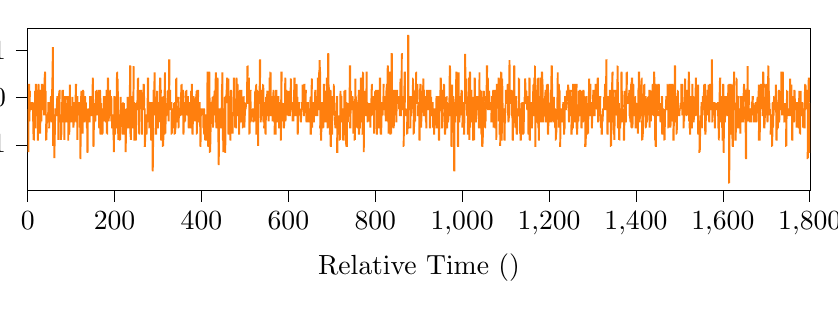
\begin{tikzpicture}[
baseline,
trim axis right,
trim axis left
]

\definecolor{color0}{rgb}{1,0.498039215686275,0.0549019607843137}

\begin{axis}[
height=0.3\textwidth,
tick align=outside,
tick pos=left,
width=0.95\textwidth,
x grid style={white!69.0196078431373!black},
xlabel={Relative Time (\si{\second})},
xmin=0, xmax=1800.934324955,
xtick style={color=black},
y grid style={white!69.0196078431373!black},
ylabel style={align=center},
ylabel={\(\displaystyle Q_{faraday}\) (\si{\pico\coulomb})},
ymin=-1.95122855, ymax=1.46485555,
ytick style={color=black},
yticklabel pos=lower
]
\addplot [semithick, color0]
table {%
0 -0.890172
0.599210530002892 -0.243187
1.20014349100529 -0.890172
0.604668883002887 -0.890172
1.20564956500311 -1.148966
1.80059134900512 -0.890172
1.80488658700051 -1.148966
2.40015559599851 0.274402
2.4044899090004 0.274402
3.00015635599993 0.274402
3.60002171800443 0.274402
3.00477137100097 -0.501981
4.20005537300312 -0.501981
3.60468447900348 -0.501981
4.79933050399995 0.145005
4.20570347700414 -0.501981
5.40010526600236 0.145005
4.80554769300215 -0.113789
6.00008943400462 -0.113789
5.40552414500416 -0.113789
6.59969108000223 -0.113789
6.00505207000242 -0.243187
7.14079292699898 -0.243187
6.60490418300469 -0.243187
7.2037514170006 -0.243187
7.80391753400181 -0.243187
7.80614374900324 -0.243187
8.4039020880009 -0.113789
8.40633957600221 -0.113789
9.00389262800309 -0.113789
9.60376314400492 -0.113789
9.0057103920044 -0.243187
9.60589269200136 -0.243187
10.2052340110022 -0.243187
10.206059119002 -0.243187
10.8046210890025 -0.113789
10.8060877989992 -0.113789
11.3100734440013 -0.113789
11.4062680120041 -0.113789
12.0061571590049 -0.113789
12.1100734440042 -0.501981
12.6060552230047 -0.113789
13.2015439009992 -0.501981
12.606648990004 -0.501981
13.2072170710017 -0.890172
13.8019237379995 -0.501981
14.4029025080017 -0.890172
13.8074959950027 -0.890172
14.4082051549995 -0.890172
15.0032442709999 -0.113789
15.0085364330007 -0.501981
15.6036267630043 -0.113789
15.6083816530008 -0.501981
16.2039221470041 -0.501981
16.8078352130033 0.145005
16.2094185489987 -0.501981
17.4078033469996 0.145005
16.8103711910007 -0.631378
17.409710179003 -0.631378
18.0093144839993 -0.631378
18.6086201380022 0.274402
18.0101490230008 -0.631378
19.0790734440016 0.274402
18.6105129190037 0.274402
19.2101270810017 -0.243187
19.8063434310025 0.274402
20.406973615005 0.015608
19.8118566330013 -0.243187
20.4118007850047 0.015608
21.0076249350022 0.015608
21.6079832169999 0.015608
21.0122718130006 -0.372584
21.6127878430052 -0.372584
22.0820734439985 -0.372584
22.2116834850021 -0.372584
22.6800734440039 0.145005
23.4088680120039 0.145005
22.8129082110027 -0.890172
23.4148056030026 -0.890172
24.009061757999 -0.890172
24.6094800819992 0.274402
24.0146682630002 -0.890172
24.6154409160008 0.274402
25.2107024350044 0.274402
25.216149576001 0.145005
25.8112068140035 0.274402
25.816120471005 -0.372584
26.411631889001 0.145005
26.4163148730004 -0.372584
26.9260734440031 -0.372584
27.0156238290001 -0.372584
27.5270734439982 0.145005
27.6154925480005 0.145005
28.0830734440024 0.145005
28.6850734440013 0.145005
28.2169365770023 -0.760775
29.2860734440037 -0.243187
28.8174149080005 -0.760775
30.0130987900047 -0.243187
29.4175243830032 -0.243187
30.6133290590005 -0.243187
30.0196176030004 -0.372584
31.2148164399987 -0.372584
30.6187859659985 -0.372584
31.2203590339996 -0.501981
31.8150027119991 -0.372584
32.4152249210019 0.274402
31.8203227470003 -0.501981
32.4211072730031 0.274402
33.0157443900025 0.274402
33.0213852540037 -0.243187
33.5320734440029 0.274402
34.1280734440006 -0.243187
33.6198015180053 -0.243187
34.7310734440034 -0.243187
34.2195266909985 -0.243187
35.3300734440054 -0.243187
34.8208756980021 -0.243187
35.8900734440031 0.015608
35.4215349689985 -0.243187
36.4880734440012 0.015608
36.0222553179992 -0.243187
36.620767694003 -0.243187
37.2171987710026 -0.243187
37.2233513860047 -0.372584
37.8182959650003 -0.243187
37.8236907200044 -0.372584
38.4185219400024 0.403799
38.4238782910033 0.403799
39.0188724399995 0.403799
39.0242108509992 0.403799
39.6194169220034 0.533196
39.6249113020021 0.533196
40.2193532640013 0.533196
40.2249561880017 0.145005
40.6930734440029 0.533196
40.8237374000018 -0.372584
41.4110734440037 0.145005
41.9360734440052 -0.372584
41.4233732180001 -0.372584
42.5390734440007 -0.372584
42.0233759930052 -0.890172
43.094073444001 -0.890172
42.6250020350053 -0.890172
43.6970734440038 -0.501981
43.2249733510034 -0.890172
44.4207369680007 -0.501981
43.825325251004 -0.501981
45.0209981299995 -0.501981
44.4268745220033 -0.501981
45.026682335003 -0.501981
45.6212183969983 -0.501981
45.6275525930032 -0.501981
46.2214838069995 -0.501981
46.2273982510014 -0.501981
46.8223811210046 -0.372584
46.8277771409994 -0.372584
47.4226542219985 -0.113789
48.0231743390032 -0.113789
47.4281039929992 -0.113789
48.623028177004 -0.113789
48.0280022410006 -0.501981
48.6282199690031 -0.501981
49.2234402950053 -0.501981
49.7020734440011 -0.501981
49.2288481659998 -0.631378
49.827638859002 -0.631378
50.3030734440035 -0.243187
50.4272700660003 -0.243187
50.9020734439982 -0.243187
51.0275100889994 -0.243187
51.5020734440041 -0.243187
52.104073444003 -0.243187
51.6290410760048 -0.243187
52.2291319270007 -0.243187
52.7460734440028 -0.113789
52.8283755410012 -0.113789
53.3010734440031 0.015608
53.4292603130016 0.015608
54.0250476910005 0.015608
54.0316643480037 -0.501981
54.6252546780015 0.015608
55.2257521409992 -0.501981
54.6308417460023 -0.501981
55.8268121830042 -0.113789
55.2315851849999 -0.501981
55.8324019350039 -0.113789
56.4270429829994 0.403799
56.9460734439999 0.403799
56.4324164900027 0.403799
57.0314908299988 0.403799
57.5460734439985 1.050784
58.1470734440009 1.050784
57.6310261590043 1.050784
58.6334739430022 1.050784
58.232566769002 -1.019569
59.3470734440052 -0.631378
58.8324083530024 -1.019569
59.4325955169988 -0.631378
60.028749776 -0.631378
60.0340433340025 -0.631378
60.6292060230044 -0.372584
60.6350512979989 -0.372584
61.2296616660024 -0.372584
61.2350940290053 -1.278363
61.8307592839992 -0.372584
62.4310725030009 -0.760775
61.8360820200032 -1.278363
62.4366364960006 -0.760775
62.956073444002 -0.760775
63.034835506005 -0.760775
63.5090734440018 -0.243187
63.6347482240017 -0.243187
64.1510734440017 -0.243187
64.7100734440028 -0.243187
64.2365330540051 -0.372584
64.8369555210011 -0.372584
65.3190734439995 -0.243187
65.4373115679991 -0.243187
65.9110734440037 -0.243187
66.037279850003 -0.243187
66.6328501500029 -0.243187
67.2331783250047 -0.243187
66.6386630179986 -0.243187
67.8335072970003 0.015608
67.2387709670002 -0.243187
67.8390780090049 0.015608
68.4338660170033 0.015608
69.0345331470016 0.015608
68.440179889003 -0.372584
69.0399408060039 -0.372584
69.634337028001 -0.113789
70.1110734440008 -0.113789
69.6404432400013 -0.113789
70.7120734440032 -0.113789
70.2388546060029 -0.890172
71.3130734439983 0.015608
70.8388732009989 -0.890172
71.440398358005 0.015608
71.9110734440037 0.015608
72.5540734440001 0.145005
72.0405794640028 0.015608
73.1160734439982 0.145005
72.6409073480027 0.145005
73.8365301750018 0.145005
73.2411517319997 -0.372584
74.436824825003 -0.372584
73.8428113590053 -0.501981
75.0371292230047 -0.501981
74.4427672829988 -0.501981
75.6375259720007 -0.372584
75.0427994560014 -0.501981
75.6435990919999 -0.372584
76.2386809279997 -0.372584
76.2436047400042 -0.890172
76.8383764270038 -0.372584
76.8446866240047 -0.890172
77.3430734440044 -0.760775
77.4431468900002 -0.760775
77.9210734439985 -0.760775
78.0426521570043 -0.760775
78.5210734440043 -0.113789
78.6440598560002 -0.113789
79.1670734440049 -0.113789
79.2445175270041 -0.113789
79.7690734440039 0.145005
79.8449740490032 0.145005
80.3220734440038 0.145005
80.4447217050038 0.145005
81.0405712030042 0.145005
81.6408507710003 0.145005
81.0460622180035 0.015608
81.6466415040049 -0.501981
82.2414109710007 0.015608
82.2466721329984 -0.501981
82.8415584300019 -0.501981
82.847331115001 -0.501981
83.4426179540023 -0.113789
83.4479355580042 -0.113789
84.0422008110036 -0.113789
84.048101846005 -0.890172
84.5270734439982 -0.113789
84.6465194289995 -0.890172
85.1490734440013 0.015608
85.7720734440009 0.015608
85.2465458600054 0.015608
86.3720734439994 0.015608
85.8480704180038 -0.372584
86.9260734440031 -0.372584
86.4485647760011 -0.372584
87.5710734439999 -0.113789
87.0479952940004 -0.372584
87.649298426004 -0.501981
88.2446972700054 -0.113789
88.8449801410025 -0.501981
88.2505845090054 -0.501981
89.446025160003 -0.501981
88.8511870840011 -0.501981
90.0457654380007 -0.501981
89.4515523630034 -0.501981
90.6462801450034 -0.243187
90.0516401749992 -0.501981
90.6524846629982 -0.243187
91.1350734439984 0.015608
91.7770734439982 0.015608
91.2509902640013 0.015608
92.3810734440049 0.015608
91.8509157740045 0.015608
92.4518319999988 0.015608
92.9370734440017 0.015608
93.5340734440033 0.015608
93.0524682360046 -0.890172
93.6528090300053 -0.890172
94.2481619020036 -0.372584
94.2536493200023 -0.372584
94.8484927040045 -0.372584
94.8537923580006 -0.760775
95.4487492769986 -0.372584
96.0490496249986 -0.760775
95.4558504540037 -0.760775
96.0557863360009 -0.760775
96.6490994830019 0.274402
96.6544949610034 -0.372584
97.2497049390004 0.274402
97.2555818820038 -0.372584
97.8499588560007 -0.372584
97.8560175150051 -0.501981
98.4510696650032 -0.372584
98.451083164 -0.501981
98.9360734440052 -0.501981
99.0545787779993 -0.501981
99.5360734440037 -0.501981
99.6544674129982 -0.501981
100.143073444 -0.372584
100.739073444005 -0.372584
100.256431300004 -0.372584
100.856372991999 -0.372584
101.382073444001 -0.243187
102.05199647 -0.243187
101.455579052999 -0.243187
102.057386 -0.243187
102.652490697001 0.015608
102.657574399003 -0.501981
103.252445704005 0.015608
103.258274737003 -0.501981
103.852877047 -0.501981
103.858465017001 -0.501981
104.453079872001 -0.243187
104.459544998004 -0.243187
105.053542456 -0.243187
105.059250696999 -0.631378
105.654445161999 -0.243187
105.659773247004 -0.631378
106.192073443999 -0.501981
106.258770291999 -0.501981
106.749073444 -0.501981
107.349073443998 -0.113789
106.858804692005 -0.501981
107.458755789004 -0.113789
107.950073444001 -0.113789
108.060142171998 -0.501981
108.551073444003 -0.113789
108.660705225004 -0.501981
109.255663241005 -0.372584
109.856002527005 -0.372584
109.261143376003 -0.372584
109.861321285003 -0.372584
110.456340058001 0.274402
110.461770735004 0.274402
111.056629543004 0.274402
111.657057827004 0.274402
111.061961763 -0.113789
112.258093584998 -0.113789
111.663506440003 -0.501981
112.858439124 -0.501981
112.263531271004 -0.501981
113.356073444003 0.015608
112.863793091004 -0.501981
113.959073443999 0.015608
113.462317411002 0.015608
114.560073444001 0.015608
114.062036563999 -0.890172
115.143073444 -0.113789
114.663761344003 -0.890172
115.859702984002 -0.113789
115.263230805998 -0.113789
115.865013310999 -0.243187
116.460008644004 -0.113789
117.060377040005 -0.243187
116.465416128005 -0.243187
117.660798736004 -0.243187
117.065783180005 -0.372584
118.261346633 -0.243187
117.666334402005 -0.372584
118.714073444004 -0.243187
118.261357378004 -0.243187
119.318073444003 -0.113789
118.861813214004 -0.243187
120.011073444002 -0.113789
119.466523996001 -0.113789
120.066438900001 -0.372584
120.570073444003 -0.113789
120.667335966005 -1.278363
121.144073444004 -0.372584
121.267740019 -1.278363
121.771073444004 -1.278363
121.868280668001 -1.278363
122.413073444004 0.015608
122.463848672 0.015608
122.969073444001 0.015608
123.064252279 0.015608
123.569073444 0.145005
123.664532134004 0.015608
124.229073444003 0.145005
124.264880152004 0.015608
124.770073444 0.015608
124.865301967002 -0.631378
125.372073443999 0.015608
125.465643736999 -0.631378
125.971073444001 -0.631378
126.069935173 -0.760775
126.615073444002 -0.631378
126.669795601003 -0.760775
127.220073444005 0.145005
127.271690414003 0.145005
127.723073444002 0.145005
127.871959741002 -0.501981
128.421073443998 0.145005
128.467506131004 -0.501981
128.976073443999 -0.501981
129.067685198999 -0.501981
129.625073444004 0.015608
129.668284113002 -0.501981
130.148073444005 0.015608
130.268574564005 -0.501981
130.781073443999 -0.501981
130.868692418 -0.501981
131.329073444002 0.015608
131.468954930002 0.015608
131.981073444003 0.015608
132.069282005003 -0.501981
132.626073444 0.015608
132.670151750004 -0.501981
133.182073444004 -0.113789
133.274423046001 -0.113789
133.782073444003 -0.113789
133.874304814002 -0.372584
134.381073444005 -0.113789
134.475411960004 -0.372584
135.027073443998 -0.372584
135.075728511001 -0.372584
135.583073444002 -0.243187
135.675949534001 -0.631378
136.183073444001 -0.243187
136.276086049002 -0.631378
136.783073443999 -0.631378
136.876503289001 -1.148966
137.382073444001 -0.631378
137.476797341005 -1.148966
137.984073444 -1.148966
138.071931031998 -1.148966
138.585073444003 -0.501981
138.671952666002 -0.501981
139.185073444001 -0.243187
139.272286076004 -0.243187
139.872491728005 -0.243187
139.878671099999 -0.501981
140.472685145003 -0.243187
140.478752530005 -0.501981
141.072895744001 -0.501981
141.078688852002 -0.501981
141.673098161998 -0.243187
141.679055239001 -0.501981
142.273352057004 -0.243187
142.278979338 -0.501981
142.786073444004 -0.501981
142.877791022001 -0.501981
143.280076135001 0.015608
143.477643505001 0.015608
143.987073444005 0.015608
144.077710825004 -0.372584
144.588073444 0.015608
144.677643037001 -0.372584
145.187073444002 -0.372584
145.279379369 -0.372584
145.788073444004 0.015608
145.879600988999 0.015608
146.388073444003 0.015608
146.479025109998 0.015608
146.989073444005 0.015608
147.079999426998 -0.243187
147.589073444004 0.015608
147.680532478 -0.372584
148.275914768004 -0.243187
148.281134165001 -0.372584
148.876233003 -0.372584
148.882914595 -0.372584
149.476549352999 0.403799
149.481906524001 0.403799
150.076604309004 0.403799
150.082142008003 0.145005
150.677131935001 0.403799
150.683679189999 -1.019569
151.277178346005 0.145005
151.283139491999 -1.019569
151.795073444002 -1.019569
152.395073444 -0.372584
151.881561006005 -1.019569
152.996073444003 -0.372584
152.481575204001 -0.372584
153.596073444001 -0.113789
153.083082499004 -0.372584
154.197073444004 -0.113789
153.683311318004 -0.243187
154.797073444002 -0.243187
154.283781413003 -0.243187
155.479425491001 -0.243187
154.883993515003 -0.501981
156.079912791 -0.501981
155.484735796999 -0.501981
156.680099862002 -0.113789
156.085153812004 -0.501981
157.280513507001 0.145005
156.685605938001 -0.113789
157.880719635003 0.145005
157.285967882002 0.145005
158.481056267003 0.145005
157.886284366003 -0.113789
159.003073444001 -0.113789
158.486657246001 -0.113789
159.602073444003 -0.113789
159.085420743002 -0.372584
160.216073444004 -0.243187
159.685427421005 -0.372584
160.804073444 -0.243187
160.285912520005 -0.243187
161.406073443999 0.015608
160.887669456002 -0.243187
161.487500169998 0.015608
162.082887274999 0.015608
162.088971782003 0.015608
162.683127891003 0.015608
162.688370240001 0.015608
163.283514891998 0.145005
163.288768885002 0.145005
163.883780159005 0.145005
163.889246929 -0.631378
164.484112470003 0.145005
164.489527209 -0.631378
165.084498340999 -0.631378
165.089778316004 -0.631378
165.684723273 0.145005
165.690353495003 0.145005
166.285063690004 0.145005
166.291071710002 0.145005
166.812073444002 0.145005
166.889891621999 -0.760775
167.412073444 0.145005
167.490006956999 -0.760775
168.015073444003 -0.760775
168.09013389 -0.760775
168.617073444002 -0.113789
168.692719798004 -0.631378
169.286870831005 -0.113789
169.292152237002 -0.631378
169.887222365003 -0.631378
170.487581746005 -0.631378
169.892532969003 -0.760775
171.087827846 -0.760775
170.492778309002 -0.760775
171.093155325005 -0.760775
171.688248897 -0.243187
172.288547001001 -0.243187
171.693876344005 -0.243187
172.293848918001 -0.760775
172.888804545 -0.243187
172.894426252999 -0.760775
173.416073444001 -0.243187
174.019073444004 -0.243187
173.493567704005 -0.243187
174.093757303999 -0.501981
174.619073444002 -0.243187
174.693349093002 -0.501981
175.216073444004 0.015608
175.816073444003 0.015608
175.294839510003 0.015608
176.424073444003 0.015608
175.895174896003 0.015608
176.494467456003 0.015608
177.090956359003 0.015608
177.691896909004 0.015608
177.096242781001 -0.243187
177.696537290001 -0.243187
178.291580771001 0.015608
178.891736799 0.015608
178.296705339002 0.015608
178.897029051004 -0.501981
179.491924351001 0.015608
179.497356803004 -0.501981
180.092613427005 -0.501981
180.692614767002 -0.501981
180.098852599003 -0.501981
181.238073444001 0.145005
180.698058915004 -0.501981
181.830073444005 0.145005
181.297307332003 0.145005
181.897623353005 -0.760775
182.428073444004 0.145005
183.031073443999 -0.760775
182.497625231001 -0.760775
183.098884693005 -0.760775
183.632073444001 -0.243187
184.235073444004 0.403799
183.699181778 -0.243187
184.836073443999 0.403799
184.299641165999 0.403799
184.899652092005 -0.243187
185.437073444002 0.403799
186.095656554004 -0.243187
185.500219476002 -0.243187
186.100870678005 -0.501981
186.695918001999 -0.243187
186.701397763005 -0.501981
187.296392852004 -0.372584
187.896605740003 -0.372584
187.301707365004 -0.372584
188.439073444002 0.145005
187.902659788 -0.372584
189.037073444 0.145005
188.501796821001 0.145005
189.670890819005 0.145005
189.101515766 -0.372584
190.242073444002 -0.372584
189.700971188999 -0.372584
190.842073444001 -0.372584
190.302733390003 -0.372584
191.499093260005 0.015608
190.902844451004 -0.372584
191.504326396003 0.015608
192.098613466005 0.015608
192.103831058004 -0.501981
192.698758908999 0.015608
193.299169966005 -0.372584
192.704032364003 -0.501981
193.305323749999 -0.372584
193.900061758999 -0.372584
194.500378069999 -0.372584
193.904636749001 -0.631378
195.099893808001 -0.631378
194.505080391005 -0.631378
195.105276437003 -0.631378
195.700128249999 -0.501981
196.300366020005 -0.372584
195.705404560002 -0.501981
196.305702831 -0.372584
196.900611602003 -0.372584
197.353073443999 -0.372584
196.906940141002 -0.760775
197.957073443999 -0.760775
197.504832203005 -0.760775
198.105361779999 -1.148966
198.557073444004 -0.760775
198.705175872004 -1.148966
199.199073444004 0.015608
199.307007879004 0.015608
199.758073444005 0.015608
199.906039633999 -0.760775
200.355073444 0.015608
200.956073444002 -0.760775
200.506980896003 -0.760775
201.107096211002 -0.760775
201.702538821002 -0.113789
201.708787493 -0.631378
202.302806420004 -0.113789
202.903058675998 -0.631378
202.308153044003 -0.631378
203.503438004998 -0.631378
202.908527079999 -0.631378
204.103815975999 -0.631378
203.508767068 -0.631378
204.704074699999 -0.501981
204.109207103 -0.631378
205.304444246001 0.533196
204.709371142999 -0.501981
205.763073444003 0.533196
205.309746596999 0.533196
206.362073444005 0.533196
205.908697453 0.403799
206.963073444 0.403799
206.508690248003 0.403799
207.109420911002 -0.760775
207.564073444002 0.403799
208.164073444001 -0.760775
207.711017226 -0.760775
208.764073443999 -0.760775
208.310567458 -0.890172
209.507154674 -0.372584
208.910161204003 -0.890172
210.106720324999 -0.372584
209.512581852003 -0.372584
210.112648640003 -0.372584
210.707067625 -0.372584
211.308251428003 -0.372584
210.712374451003 -0.631378
211.313059986001 -0.631378
211.907776143002 -0.631378
212.508232573004 -0.631378
211.913147817002 -0.890172
213.108427918 -0.890172
212.513709980005 -0.890172
213.570073444003 0.015608
213.114638872001 -0.890172
214.255073444001 0.015608
213.712511432001 -0.243187
214.814073444002 -0.243187
214.315014871005 -0.243187
214.915324159003 -0.372584
215.414073444001 -0.243187
215.514597068002 -0.372584
215.973073444002 -0.372584
216.115046461004 -0.372584
216.710327790002 -0.113789
216.717171822005 -0.501981
217.311483022 -0.113789
217.316879351005 -0.501981
217.910957372005 -0.501981
217.916662073003 -0.760775
218.511115991001 -0.501981
218.516402542002 -0.760775
219.112481159005 -0.760775
219.117981821 -0.760775
219.712439587005 -0.113789
219.718097466 -0.113789
220.312904617 -0.113789
220.91232974 -0.113789
220.317333257 -0.113789
220.917872585 -0.760775
221.512376756 -0.113789
221.517785182004 -0.760775
222.018073444 -0.760775
222.619073444002 -0.243187
222.117322131999 -0.760775
223.273073444005 -0.243187
222.716604453002 -0.501981
223.823073444 -0.501981
223.316856973004 -0.501981
224.428073444004 -0.372584
223.919257852001 -0.501981
224.518081204005 -0.372584
225.023073444005 -0.372584
225.581073444002 -0.372584
225.119257081999 -1.148966
226.183073444001 -0.631378
225.718580200002 -1.148966
226.822073444004 -0.631378
226.318653091999 -0.631378
227.515532685 -0.243187
226.918917770003 -0.631378
228.114928218005 -0.243187
227.520777634003 -0.243187
228.120421716005 -0.501981
228.715096644002 -0.243187
228.720404801003 -0.501981
229.316384862002 -0.501981
229.915604608002 0.015608
229.321675753003 -0.501981
230.515887134003 0.015608
229.922081811004 -0.631378
230.522328265004 -0.631378
231.115971979001 -0.631378
231.589073444004 -0.372584
231.121391715998 -0.631378
232.320503631003 -0.372584
231.720901549001 -0.631378
232.323129825003 -0.631378
232.792073444005 -0.631378
233.428073444004 0.015608
232.921838341004 -0.631378
233.993073443999 0.015608
233.522050676002 0.015608
234.628073444001 0.015608
234.122379123 -0.501981
234.723479403001 -0.501981
235.319220256002 0.662593
235.323554622999 0.662593
235.918974762004 0.662593
235.924302865002 -0.760775
236.519079205005 0.662593
237.120396413004 -0.760775
236.525298510001 -0.760775
237.124637271001 -0.890172
237.719691793005 -0.760775
237.725305316999 -0.890172
238.320027993999 -0.243187
238.325376604 -0.243187
238.799073444003 -0.243187
239.399073444001 0.015608
238.924745215001 -0.243187
239.999073444 0.015608
239.524841530001 0.015608
240.600073444002 0.015608
240.126438093001 -0.113789
240.726342351001 -0.631378
241.237073444005 -0.113789
241.834073443999 -0.631378
241.325995879 -0.631378
242.404073443999 -0.501981
241.926366312 -0.631378
243.121840054002 -0.501981
242.526537415004 -0.501981
243.723160316003 0.662593
243.128016477 -0.501981
244.323447139999 0.662593
243.727582967003 -0.113789
244.922657175004 -0.113789
244.328734173003 -0.113789
245.523122760002 -0.113789
244.929020674004 -0.890172
246.123184476004 -0.890172
245.528651355002 -0.890172
246.723329594999 -0.113789
246.129497219001 -0.890172
247.323581346005 -0.113789
246.729583556 -0.501981
247.329013488001 -0.501981
247.924513010999 -0.501981
247.928970705005 -0.890172
248.524569493005 -0.501981
248.529286632998 -0.890172
249.123880163999 -0.890172
249.729164848999 -0.243187
249.129637623999 -0.890172
250.328420278005 -0.243187
249.729931536 -0.243187
250.330041214998 -0.243187
250.930011683005 -0.243187
251.530281965999 -0.113789
251.128656198001 -0.243187
251.728187786 -0.113789
252.128325313999 -0.113789
252.130959996 -0.113789
252.729360005003 0.015608
253.330490756001 0.403799
252.731486870005 0.015608
253.931274022005 0.403799
253.332017200999 0.403799
254.531482445003 0.403799
254.048073443999 0.015608
254.654073443999 0.015608
255.130915435999 0.015608
255.732075582004 -0.760775
255.197073444004 -0.760775
255.851073443999 -0.760775
256.331120011004 -0.760775
256.386073444002 0.145005
256.932119885001 0.145005
257.531537993003 0.145005
257.051073444003 -0.243187
258.131950881005 -0.243187
257.655073444002 -0.243187
258.732673707003 -0.113789
258.257073444001 -0.243187
259.332976500998 -0.113789
258.821073444 -0.113789
259.932992080001 -0.113789
259.456073444002 -0.113789
260.061073444005 -0.113789
260.532121525001 0.145005
261.132291763002 0.145005
260.656073443999 0.145005
261.733324346998 0.145005
261.222073444005 -0.113789
261.821073444 -0.760775
262.332638190004 -0.113789
262.460073444003 -0.760775
262.933515952005 -0.760775
263.064073444002 -0.760775
263.532814871003 0.015608
264.133131497001 0.015608
263.623073444003 0.015608
264.224073443998 -0.113789
264.733212607003 0.015608
264.865073444002 -0.243187
265.333622677004 -0.113789
265.933662283998 -0.243187
265.425073443999 -0.243187
266.534171517 0.274402
266.068073444003 -0.243187
267.133810804 0.274402
266.664073444001 0.274402
267.269073444004 -0.113789
267.735037273 0.274402
268.334870138002 -0.113789
267.830073444005 -0.243187
268.935003223 -0.243187
268.467073444001 -0.243187
269.535482842999 -0.243187
269.068073444003 -1.019569
269.631073444005 -1.019569
270.134753580998 -1.019569
270.734719100001 -0.631378
270.268073444 -1.019569
271.335391035005 -0.372584
270.868073443999 -0.631378
271.433073444001 -0.372584
271.935051918001 -0.372584
271.998341039005 -0.760775
272.535130299999 -0.372584
272.676073444003 -0.760775
273.135481042002 -0.760775
273.736205146 -0.760775
273.235073444004 -0.760775
273.873073444003 -0.760775
274.335438521004 -0.372584
274.936730364003 -0.372584
274.436073444005 -0.372584
275.535752856005 -0.372584
275.072073444004 -0.501981
276.13684608 -0.501981
275.672073444002 -0.501981
276.218073444004 0.403799
276.737151491005 0.403799
276.875073444004 0.403799
277.336438283004 0.403799
277.937793317004 -0.113789
277.382073444001 -0.113789
278.536370459005 -0.113789
278.038073444004 -0.501981
279.136919755001 -0.501981
278.676073444003 -0.501981
279.241073444005 -0.501981
279.737328688003 -0.243187
280.337585934001 -0.243187
279.876073444 -0.631378
280.937997781002 -0.631378
280.477073444003 -0.631378
281.537590209002 -0.113789
281.041073444001 -0.631378
281.675073443999 -0.113789
282.138263594003 -0.113789
282.182073444004 -0.501981
282.737644184002 -0.113789
282.846073444001 -0.501981
283.337606907 -0.113789
283.447073444004 -0.113789
283.937758826003 -0.113789
283.985073444004 -0.890172
284.539445854003 -0.113789
284.586073443999 -0.890172
285.138281983003 -0.890172
285.240073444002 -0.113789
285.739569853999 -0.113789
285.784073444003 -0.113789
286.339742855002 -0.113789
286.386073444002 -0.113789
286.938549012004 -0.113789
286.985073444004 -1.537158
287.539095493004 -0.113789
287.586073443999 -1.537158
288.138659715005 -1.537158
288.184073444005 -1.537158
288.739785127 -1.019569
288.856073444003 -1.019569
289.339666979002 0.145005
289.487073444005 0.145005
289.939785092 0.145005
290.058073444001 0.145005
290.539820837999 0.145005
290.660073444 0.145005
291.139419505998 0.145005
291.259073444002 0.145005
291.739920805005 0.533196
291.859073444 -0.113789
292.339587441005 0.533196
292.940086979004 -0.113789
292.487073444005 -0.113789
292.992073444002 -0.372584
293.539530644004 -0.113789
294.139540703 -0.372584
293.688073443998 -0.372584
294.295073444002 -0.372584
294.739657115002 -0.372584
295.339735157002 -0.372584
294.793073444001 -0.760775
295.467073444001 -0.760775
295.940430786999 -0.760775
296.541100728005 -0.113789
296.094073444001 -0.760775
297.139854304005 -0.113789
296.734427919 -0.113789
297.740271192 0.145005
297.296073443998 -0.113789
297.895073444 -0.501981
298.350073444002 0.145005
298.939906625004 -0.501981
298.474073443998 -0.501981
299.540036004 -0.501981
299.074073444004 -0.631378
299.673073443999 -0.631378
300.140629762005 -0.631378
300.193073444003 -0.631378
300.740020734003 -0.113789
301.340766257003 -0.113789
300.796073443998 -0.501981
301.940952271005 -0.501981
301.395073444 -0.501981
301.996073444003 -0.501981
302.540515499 -0.501981
302.583073444002 -0.501981
303.141276337003 -0.501981
303.741885619005 -0.501981
303.198073444 -0.501981
304.341930577 0.403799
303.882073444001 -0.501981
304.942209754001 0.403799
304.399073444001 0.403799
304.984073444 0.145005
305.541354165005 0.403799
306.142176551999 0.145005
305.599073443998 0.145005
306.741990763003 0.145005
306.199073444004 -0.243187
306.842073444001 -0.890172
307.344407772005 -0.243187
307.388073444003 -0.890172
307.94334826 -0.890172
308.543102834003 -0.372584
308.047073444002 -0.890172
309.142899842001 -0.372584
308.646073444004 -0.372584
309.202073444001 -0.760775
309.742787977004 -0.372584
310.343811289 0.015608
309.794073444005 -0.760775
310.944213788003 0.015608
310.404073443999 0.015608
311.543748835 0.015608
311.008073444005 -1.019569
312.144680885001 -1.019569
311.638073444003 -1.019569
312.745089976001 -0.372584
312.196073444 -1.019569
313.345256339999 -0.372584
312.795073444002 -0.631378
313.945650498004 -0.631378
313.395073444 -0.631378
314.544918671003 -0.113789
313.996073444003 -0.631378
315.145409853001 -0.113789
314.597073444005 -0.113789
315.746817125 0.533196
315.199073444004 -0.113789
316.346574607 0.533196
315.844073444001 -0.760775
316.946146348004 -0.760775
316.457073443999 -0.760775
317.546836845002 -0.372584
316.999611940999 -0.760775
318.147059506002 -0.372584
317.611073444001 -0.372584
318.747390675002 -0.113789
318.246073444003 -0.372584
319.347915040998 -0.113789
318.859073444 -0.243187
319.403073444002 -0.243187
319.948000276003 -0.243187
320.547867497 -0.243187
320.046073443998 -0.372584
321.148602601002 -0.372584
320.648073444005 -0.372584
321.748926208005 0.145005
321.262073443999 0.145005
322.349376572005 0.145005
321.804073444 0.145005
322.424073444003 0.145005
322.949296636005 0.145005
323.022073444001 0.145005
323.549507677999 0.145005
323.609073444 0.145005
324.149694723004 0.145005
324.223073444002 -0.501981
324.750612510004 0.145005
324.812073444002 -0.501981
325.350695305002 0.79199
325.466073444004 0.79199
325.950479220999 0.79199
326.550821517005 0.79199
326.013073444003 -0.113789
327.151079952004 -0.113789
326.670073444002 -0.113789
327.751641616 0.145005
327.230073444 0.145005
328.352112288005 0.145005
327.770907466998 -0.243187
328.430073444004 -0.243187
328.952185599002 -0.243187
329.015073444003 -0.243187
329.551827373005 -0.113789
330.152838881004 -0.113789
329.675073443999 -0.113789
330.753152060999 -0.113789
330.262073443999 -0.113789
331.353224731 -0.113789
330.858073444004 -0.760775
331.952774096004 -0.760775
331.484073444 -0.760775
332.552736030004 -0.501981
332.043073444001 -0.760775
333.153080308999 -0.501981
332.662073444 -0.501981
333.753414327002 -0.243187
333.263073444003 -0.243187
334.353939660999 -0.243187
333.820073444003 -0.372584
334.953910194999 -0.372584
334.440073443999 -0.372584
335.553874509002 -0.372584
335.088073444 -0.631378
336.154403831002 -0.631378
335.667073444005 -0.631378
336.754917659004 -0.113789
336.229073444003 -0.113789
337.354237865999 -0.113789
336.888073444003 -0.113789
337.955376897 -0.113789
337.468073444004 -0.113789
338.555038658 -0.113789
338.043073444001 -0.760775
339.154763908002 -0.760775
338.689073444002 -0.760775
339.755379603004 -0.631378
339.291073444001 -0.760775
340.355554624002 -0.631378
339.847073444005 -0.631378
340.955462506005 -0.631378
340.470073444005 -0.631378
341.555841351001 0.403799
341.047073444002 -0.631378
342.155886706001 0.403799
341.647073444001 0.403799
342.756024887 0.403799
342.230073444 -0.243187
343.356880922998 -0.243187
342.893073444 -0.501981
343.496073444003 -0.501981
343.956679278999 -0.501981
344.556497180005 -0.243187
344.049073444003 -0.501981
345.157006448004 -0.243187
344.679073444 -0.243187
345.256073444005 -0.501981
345.757233830998 -0.243187
345.954531898999 -0.501981
346.358201353003 -0.501981
346.957430372 0.015608
346.438073443998 -0.501981
347.557388100002 0.015608
347.095073444005 -0.631378
348.157830206001 -0.631378
347.638073444003 -0.631378
348.235073444004 -0.372584
348.757812929005 -0.372584
348.850073444002 -0.372584
349.358038167004 -0.243187
349.454073444002 -0.243187
349.957402541004 -0.243187
350.054073444 -0.372584
350.557541344999 -0.243187
350.654073443999 -0.372584
351.158324921002 -0.372584
351.758886996999 -0.243187
351.243073443999 -0.372584
352.358205582001 -0.113789
351.855073444 -0.243187
352.958315511001 -0.113789
352.404073443999 -0.113789
353.559002510003 0.274402
353.004073444004 -0.113789
354.158444893001 0.274402
353.700073444001 0.274402
354.758815226 0.274402
354.256073444005 -0.372584
355.358889571005 -0.113789
354.859073444 -0.372584
355.552903087999 -0.113789
355.958612882001 -0.113789
356.006073444005 -0.243187
356.558635324 -0.113789
356.692073443999 -0.243187
357.159412330999 -0.243187
357.241073444005 0.145005
357.759659221003 0.145005
357.808073444001 -0.760775
358.359986486001 0.145005
358.460073444003 -0.760775
358.959957481005 -0.760775
359.009073444002 -0.760775
359.559590833 -0.113789
359.651073444002 -0.113789
360.160285671001 -0.113789
360.295073444002 -0.372584
360.760243563003 -0.113789
361.360616256003 -0.372584
360.897073444001 -0.372584
361.960487646 -0.372584
361.558695856002 -0.372584
362.560597674004 -0.372584
362.109073444 -0.501981
363.161036030004 -0.501981
362.662073444 -0.501981
363.760991376002 0.015608
363.244073444002 0.015608
364.360334791003 0.145005
363.867073444002 0.015608
364.961247257001 0.145005
364.503073444001 0.145005
365.560947513004 0.145005
365.059073444005 -0.113789
366.161487039004 -0.113789
365.615073444002 -0.113789
366.761724329001 -0.113789
366.267073444003 -0.372584
367.362007618001 -0.113789
366.868073443999 -0.372584
367.962220746005 -0.113789
367.466073444004 -0.113789
368.561281890004 0.015608
368.112073444005 -0.113789
368.664073444001 0.015608
369.162383688003 0.015608
369.244073444002 -0.372584
369.762346077005 -0.372584
369.865073444002 -0.631378
370.361663053001 -0.372584
370.468073444004 -0.631378
370.962461023002 -0.631378
371.014073443999 -0.631378
371.562665739002 -0.372584
371.666073444001 -0.372584
372.162557117001 -0.372584
372.220073444005 -0.372584
372.762538536001 -0.113789
372.819073444 -0.113789
373.362935516001 -0.113789
373.415073444005 -0.631378
373.962938110999 -0.631378
374.071073444 -0.631378
374.562901636004 -0.501981
374.671073443998 -0.501981
375.162745112 -0.501981
375.216073444004 -0.501981
375.763101461001 0.145005
375.816073444003 -0.501981
376.363087350001 0.145005
376.515073444003 -0.501981
376.963142355999 -0.501981
377.071073444 -0.501981
377.563147387998 0.274402
377.675073443999 0.274402
378.163273857004 0.274402
378.252073444004 0.015608
378.763220509005 0.015608
378.876073444 -0.760775
379.363268820001 0.015608
379.519073444004 -0.760775
379.963416359999 -0.760775
380.562781076005 0.015608
380.023073444005 -0.760775
381.163400598001 0.015608
380.724073443998 0.015608
381.763729361999 0.015608
381.276073444002 -0.372584
382.363669488004 -0.243187
381.878073444001 -0.372584
382.963747597001 -0.243187
382.479073444003 -0.243187
383.563763835999 -0.113789
383.024073444001 -0.243187
384.163651178998 -0.113789
383.723073444002 -0.113789
384.764003845004 -0.113789
384.229073444003 -0.501981
385.364160982004 -0.243187
384.883073444005 -0.501981
385.964200977003 -0.243187
385.530073444002 -0.243187
386.563793214998 0.015608
386.085073444003 -0.243187
387.164370589002 0.015608
386.687073444002 0.015608
387.764835314003 0.015608
387.289073444001 -0.243187
388.364390808005 0.145005
387.888073444003 -0.243187
388.964528665005 0.145005
388.485073444004 0.145005
389.565108077004 0.145005
389.129359295002 -0.760775
390.165306473005 -0.760775
389.731073444003 -0.760775
390.7643685 -0.243187
390.276073444002 -0.243187
391.364740088 0.145005
390.887073443999 -0.243187
391.965203947002 0.145005
391.532073444003 0.145005
392.565228217005 0.145005
392.088073444 -0.243187
392.689073444002 -0.243187
393.165292123005 -0.243187
393.290073444005 -0.501981
393.765535067003 -0.243187
393.892073444003 -0.501981
394.366183038001 -0.501981
394.435073444001 -0.243187
394.966242130002 -0.243187
395.136073444002 -0.243187
395.566475198 -0.113789
395.639073443999 -0.113789
396.167205543999 -0.113789
396.257073444001 -0.243187
396.767830279001 -0.243187
396.835073444003 -1.019569
397.367484284005 -0.243187
397.492073444002 -1.019569
397.967604506004 -1.019569
398.092073444001 -1.019569
398.567572616004 -0.372584
398.694073444 -0.372584
399.168219496001 -0.372584
399.295073444002 -0.372584
399.768925281001 -0.243187
399.895073444 -0.243187
400.369047483 -0.243187
400.496073444003 -0.243187
400.968816262 -0.243187
401.096073444001 -0.243187
401.568891272 -0.243187
401.695073444003 -0.243187
402.169052299003 -0.243187
402.295073444002 -0.243187
402.770304631005 -0.243187
402.896073444004 -0.243187
403.370708212002 -0.243187
403.495073443999 -0.243187
403.970796874004 -0.243187
404.096073444001 -0.631378
404.570300468004 -0.243187
404.700073444001 -0.631378
405.171203269005 -0.631378
405.265073444003 -0.243187
405.771439092001 -0.243187
405.903073444002 -0.760775
406.371764285999 -0.243187
406.503073444001 -0.760775
406.972049344004 -0.760775
407.103073443999 -0.760775
407.572757362002 -0.501981
407.703073444005 -0.501981
408.172160003 -0.501981
408.304073444 -0.890172
408.773236150999 -0.501981
408.906073443999 -0.890172
409.373673686001 -0.890172
409.506073444005 -0.890172
409.973936362003 -0.890172
410.106073444003 -0.890172
410.572967395005 -0.372584
410.711073443999 -0.372584
411.173610903003 -0.372584
411.271073444004 -0.890172
411.773471938002 -0.890172
411.817073443999 -0.890172
412.372814981005 -0.631378
412.417073444005 -0.631378
412.980894660999 -0.631378
413.108073444004 -0.631378
413.573008905005 0.533196
413.622073443999 0.533196
414.173156239005 0.533196
414.217073444001 -0.113789
414.773460028999 0.533196
414.826073444005 -1.019569
415.372781894002 -0.113789
415.424073444003 -1.019569
415.972887447999 -1.019569
416.023073444005 -1.019569
416.572882859 0.403799
416.620073443999 0.403799
417.210419708004 0.403799
417.252073444004 0.533196
417.773503272001 0.533196
417.823073444 -0.113789
418.372881759999 0.533196
418.972779610005 -0.113789
418.428073444004 -0.113789
419.616073444005 -0.113789
419.027073443998 -1.148966
420.172750087004 -1.148966
419.767406853003 -1.148966
420.817073443999 -0.631378
420.225073444002 -1.148966
421.372560053998 -0.631378
420.967640991999 -0.631378
421.973687837999 -0.501981
421.427073444 -0.631378
422.573005080005 -0.113789
422.027073443998 -0.501981
423.217073444001 -0.113789
422.631073444005 -0.113789
423.772291088004 -0.501981
423.280073444002 -0.501981
424.372581118005 -0.113789
423.835073444003 -0.501981
424.972338236999 -0.113789
424.566771853002 -0.113789
425.619073444002 0.015608
425.030073444002 -0.113789
426.172814893005 0.015608
425.766789310001 0.015608
426.772305929 0.015608
426.231073444003 -0.631378
427.399756162005 -0.113789
426.832073443999 -0.631378
427.972165251005 -0.113789
427.440073443999 -0.113789
428.573109050005 -0.113789
428.036073444004 -0.372584
429.171603670999 -0.372584
428.639073443999 -0.372584
429.772260160003 0.145005
429.238073444001 -0.372584
430.372056551001 0.145005
429.839073444004 0.145005
430.972316251005 0.145005
430.443073444003 0.145005
431.572062769999 0.145005
431.024073444001 0.015608
432.172163000003 0.015608
431.625073444004 0.015608
432.771859474 0.533196
432.243073443999 0.015608
433.37262953 0.533196
432.842073444001 -0.501981
433.427073444 -0.501981
433.971995418004 -0.501981
434.047073444002 -0.631378
434.572068002002 -0.501981
434.646073444004 -0.631378
435.172035740005 -0.631378
435.246073444003 -0.631378
435.771842932001 -0.501981
435.831073444002 -0.501981
436.371835479003 0.403799
436.432073444004 0.403799
436.972332299003 0.403799
437.047073444002 -0.631378
437.572187185004 0.403799
437.650073444005 -0.631378
438.172484727002 -0.631378
438.234073444 -0.631378
438.772558281002 -0.501981
438.836073443999 -1.40776
439.371772261999 -0.501981
439.435073444001 -1.40776
439.972161669 -1.40776
440.051073444003 -1.40776
440.571419347005 -0.631378
440.651073444002 -0.631378
441.171399611005 -0.631378
441.236073444001 -0.243187
441.771950886003 -0.243187
441.837073444003 -0.243187
442.371325124004 -0.243187
442.439073444002 -0.243187
442.971393275002 -0.243187
443.051073444003 -0.631378
443.571224218002 -0.243187
443.655073444002 -0.631378
444.171288234 -0.631378
444.252073444004 -0.631378
444.771195314999 -0.372584
444.855073444 -0.501981
445.371440966999 -0.372584
445.443073444003 -0.501981
445.970635293001 -0.501981
446.042073444005 -0.501981
446.570399465003 0.145005
446.655073444002 0.145005
447.170244676003 0.145005
447.244073444002 0.145005
447.770586046005 0.533196
447.858073444004 -0.243187
448.370163222004 0.533196
448.454073444002 -0.243187
448.970508634004 -0.243187
449.058073444001 -0.890172
449.569955076004 -0.243187
449.655073444002 -0.890172
450.169652121003 -0.890172
450.251073444 -1.148966
450.770490392002 -0.890172
450.858073444004 -1.148966
451.369628894005 -0.890172
451.458073444002 -0.890172
451.969801753003 -0.890172
452.054073444 -0.890172
452.569540130004 -0.631378
452.651073444002 -0.631378
453.169481443001 -0.631378
453.258073444005 -0.631378
453.769648308 0.015608
453.858073444004 -1.148966
454.369748595003 0.015608
454.458073444002 -1.148966
454.970202597004 -1.148966
455.054073444 -1.148966
455.569445646004 0.015608
455.658073443999 0.015608
456.170510655 0.015608
456.262073443999 -0.113789
456.770684360999 0.015608
456.866073444005 -0.113789
457.370572858999 0.145005
457.455073444005 0.145005
457.970676244004 0.145005
458.062073444002 0.145005
458.570204050004 0.403799
458.666073444001 0.403799
459.170720524999 0.403799
459.239073444005 0.015608
459.769907318005 0.015608
459.866073444005 0.015608
460.370468708999 0.015608
460.459073443999 0.015608
460.970479624004 0.015608
461.067073443999 0.015608
461.571101639005 0.403799
461.661073444004 -0.760775
462.235073444004 0.403799
462.368791141998 -0.760775
462.771408689005 -0.760775
462.866073444005 -0.760775
463.370891514001 -0.631378
463.467073444001 -0.631378
463.971092393003 -0.631378
464.075073444001 -0.631378
464.570330697999 0.015608
464.670073444002 0.015608
465.170832283999 0.015608
465.271073444004 -0.113789
465.770940925999 0.015608
465.873073444003 -0.890172
466.370971927005 -0.113789
466.449004362999 -0.890172
466.970912936005 -0.890172
467.075073444001 -0.890172
467.570806071999 0.145005
467.675073443999 0.145005
468.180358329999 0.145005
468.278073444002 -0.372584
468.770199307 0.145005
468.878073444001 -0.372584
469.370834658002 -0.372584
469.488073444001 -0.372584
469.969879802004 -0.372584
470.082073443999 -0.501981
470.569712707998 -0.372584
470.679073444 -0.501981
471.170776965999 -0.501981
471.283073443999 -0.760775
471.770393522005 -0.501981
471.888073444003 -0.760775
472.370003573 -0.372584
472.478073443999 -0.372584
472.969516322002 -0.372584
473.083073444002 -0.372584
473.569268038002 -0.243187
473.679073444 -0.243187
474.235073444004 0.403799
474.287073444 0.403799
474.769068665999 0.403799
474.897073444001 -0.113789
475.368718064004 0.403799
475.491073444005 -0.113789
475.968662008003 -0.113789
476.091073444004 -0.243187
476.568491303005 -0.113789
476.692073443999 -0.243187
477.168291212001 -0.243187
477.294073444005 -0.631378
477.768257651005 -0.243187
477.896073444004 -0.631378
478.368111948002 -0.501981
478.490073444002 -0.501981
478.967858595999 -0.501981
479.082073443999 -0.631378
479.567837210001 -0.501981
479.696073444 -0.631378
480.167583220005 -0.631378
480.275073444005 0.403799
480.767558140004 0.403799
480.895073444 -0.372584
481.367335802999 0.403799
481.499073444 -0.372584
481.967602868004 -0.372584
482.100073444002 -0.372584
482.567620016998 0.274402
482.761946416998 0.274402
483.167296174004 0.274402
483.300073443999 0.145005
483.767903843 0.274402
483.961941589005 -0.372584
484.367516286999 0.145005
484.500073444004 -0.372584
484.966628836999 -0.372584
485.088073444 -0.372584
485.566699170005 0.015608
485.690073443999 0.015608
486.209073443999 0.015608
486.264073443999 -0.760775
486.767040938001 -0.760775
486.966199711002 -0.760775
487.409073444003 -0.501981
487.566327345005 -0.501981
488.009073444002 -0.501981
488.166231504001 -0.501981
488.616073444005 0.145005
488.766044021999 0.145005
489.210073444003 0.145005
489.283073443999 0.015608
489.767836255 0.015608
489.907073444003 -0.501981
490.413073444004 0.015608
490.565969666 -0.501981
490.966991391004 -0.501981
491.100073444002 -0.501981
491.615073444002 0.145005
491.766138332001 0.145005
492.167069326002 0.145005
492.281073443999 0.015608
492.768057736001 0.015608
492.903073444002 -0.501981
493.366744627005 0.015608
493.512073443999 -0.501981
494.019073444004 -0.501981
494.165825945005 -0.501981
494.617073444002 -0.243187
495.243073443999 -0.243187
494.765894256001 -0.631378
495.818073444003 -0.631378
495.366054532999 -0.631378
496.420073444002 0.015608
495.965217978999 -0.631378
497.010073443998 0.015608
496.566029778005 0.015608
497.567490804002 0.015608
497.165963631 -0.113789
498.219073444001 -0.113789
497.718073444004 -0.113789
498.817073443999 -0.113789
498.366129531001 -0.631378
499.414073444001 -0.372584
498.966063119005 -0.631378
500.016073444 -0.372584
499.565695069999 -0.372584
500.615073444002 -0.113789
500.162314916 -0.372584
501.242073444002 -0.113789
500.761734854001 -0.243187
501.817073443999 -0.243187
501.362531463004 -0.243187
502.423073443999 -0.113789
501.962027624002 -0.243187
503.023073444005 -0.113789
502.561991864 -0.113789
503.620073443999 -0.113789
503.162253720002 -0.113789
504.220073444005 -0.113789
503.762496064002 -0.113789
504.820073444003 -0.113789
504.362489726002 -0.113789
505.422073444002 0.662593
504.962486967001 -0.113789
506.025073444005 0.662593
505.563376805003 0.662593
506.627073444004 0.662593
506.065941951005 0.274402
507.253073444001 0.274402
506.763564788998 -0.113789
507.824073444004 -0.113789
507.362610738004 -0.113789
508.428073444004 0.403799
507.962611923002 -0.113789
509.025073444005 0.403799
508.562372307999 0.403799
509.624073444 0.403799
509.162401089001 0.015608
510.236073444001 0.015608
509.762434384 -0.760775
510.832073443999 -0.760775
510.362493380002 -0.760775
511.438073443998 0.015608
510.962418689 -0.760775
512.028073444002 0.015608
511.562277650999 0.015608
512.629073444004 0.145005
512.162377318004 0.015608
513.229073444003 0.145005
512.762370740005 0.145005
513.834073443999 -0.372584
513.278073444002 -0.372584
514.433073444001 -0.372584
513.962491607002 -0.501981
515.034073444003 -0.501981
514.562621896002 -0.501981
515.637073443999 -0.372584
515.162476477999 -0.501981
516.255073444001 -0.243187
515.762680662003 -0.372584
516.835073444003 -0.243187
516.363410196005 -0.243187
517.439073444002 -0.243187
516.962713313005 -0.372584
518.041073444001 -0.372584
517.562439663001 -0.372584
518.640073444003 -0.243187
518.162617893002 -0.372584
519.241073444005 -0.243187
518.762565265002 -0.243187
519.768831491005 -0.243187
519.362607276998 -0.243187
520.442073443999 -0.243187
519.882073444001 -0.501981
520.968137871001 -0.501981
520.562506388 -0.501981
521.630073444001 -0.501981
521.088073444 -0.501981
522.262073443999 -0.243187
521.762691479998 -0.501981
522.768311170999 -0.243187
522.362571515005 -0.243187
523.447073444004 0.145005
522.891073444 -0.243187
523.967838338998 0.145005
523.562507032002 0.145005
524.638073444003 0.145005
524.091073444004 0.145005
525.167573065999 0.145005
524.762278786999 0.145005
525.834073443999 0.274402
525.314073444002 0.274402
526.398073444005 0.274402
525.962326596004 -0.760775
526.967576813004 -0.760775
526.540073444005 -0.760775
527.637073443999 -0.760775
527.136073444002 -0.760775
528.167253582003 -0.760775
527.762044144001 -0.760775
528.767877089005 -0.372584
528.291073444001 -0.760775
528.896073444004 -0.372584
529.367662540004 0.145005
529.967014056005 0.145005
529.496073444003 0.145005
530.096073444001 -1.019569
530.566788135999 0.145005
530.741073444005 -1.019569
531.243073443999 -0.113789
531.362034718004 -0.113789
531.767469404003 -0.113789
532.461073443999 -0.113789
531.897073444001 -0.113789
532.560953284999 -0.113789
532.967225105 -0.113789
533.095073444005 -0.113789
533.642073444003 0.145005
534.252073444004 0.79199
533.765917315999 0.145005
534.365544061002 0.79199
534.766439065002 0.79199
535.366743269005 0.79199
534.898073444005 0.145005
536.048073443999 0.145005
535.497073443999 0.145005
536.5656074 0.145005
536.164982400005 -0.501981
536.701073444005 -0.501981
537.263073444003 -0.372584
537.363979986003 -0.372584
537.848073444002 -0.372584
538.365647448001 0.015608
537.963482151004 -0.372584
538.966308089002 0.015608
538.502073444004 0.015608
539.650073444005 0.015608
539.101073443999 -0.113789
539.722255518005 -0.113789
540.207073443999 -0.113789
540.851073443999 0.145005
540.339073444004 0.145005
540.963910292005 0.145005
541.452073444001 0.274402
542.030793875005 0.274402
541.563966547001 0.274402
542.163914955003 -0.501981
542.565386360002 0.274402
542.704073444002 -0.501981
543.165877766005 -0.501981
543.813073443998 -0.501981
543.304073444 -0.501981
544.459073443999 -0.501981
543.963983788002 -0.631378
544.563165306005 -0.631378
545.013073444003 -0.631378
545.163925581001 -0.631378
545.655073444002 -0.113789
545.763496596999 -0.113789
546.255073444001 -0.113789
546.365028084001 -0.631378
546.808073444001 -0.113789
546.965168750001 -0.760775
547.412073444 -0.631378
547.565268056998 -0.760775
548.054073444 -0.760775
548.165759251999 -0.760775
548.616073444005 0.015608
548.766158275001 -0.372584
549.265073444003 0.015608
549.365593684 -0.372584
549.767027144 -0.372584
550.411073444004 0.015608
549.911073444004 -0.372584
550.967658948 0.015608
550.566044480998 0.015608
551.567377300998 0.145005
551.110073444004 0.015608
552.284073444003 0.145005
551.712073444003 -0.372584
552.361422024005 -0.372584
552.819073444 -0.372584
552.961598460002 -0.372584
553.419073444005 0.015608
553.561821742005 0.015608
554.018073444 0.015608
554.162290491004 -0.501981
554.631073444005 0.015608
554.761966235004 -0.501981
555.270073444 -0.372584
555.362174522001 -0.372584
555.767554329002 -0.372584
555.962370734 -0.372584
556.462073444003 0.403799
556.562463911003 0.403799
557.067073443999 0.403799
557.624073444 0.403799
557.16260612 0.015608
557.763008708003 0.015608
558.233073444004 0.533196
558.866073444005 0.533196
558.326073444005 0.533196
558.967512798001 -0.372584
559.425073443999 0.533196
559.567679788001 -0.372584
560.029073443999 -0.372584
560.168485266004 -0.372584
560.670073444002 0.015608
561.271073444004 0.015608
560.769403978004 0.015608
561.828073444005 0.015608
561.369056987001 -0.243187
562.439073444002 -0.243187
561.968553724 -0.243187
562.570002458 -0.243187
563.030073444002 -0.243187
563.671073443998 -0.243187
563.164865529005 -0.501981
564.252073444004 -0.113789
563.765179186004 -0.501981
564.365410090999 -0.113789
564.771039418003 -0.113789
565.479073444003 0.145005
564.966081936 -0.113789
566.044073444005 0.145005
565.566271650001 0.145005
566.166381802999 -0.372584
566.634073444002 0.145005
567.172276249999 -0.372584
566.766693730999 -0.372584
567.315073443999 -0.501981
567.832073443999 -0.501981
568.431073444001 -0.501981
567.971658677001 -0.760775
568.571175016004 -0.760775
569.075073444001 -0.760775
569.675073443999 -0.760775
569.172656953 -0.760775
570.233073444004 -0.760775
569.772991764003 -0.760775
570.373060786005 -0.760775
570.878601021999 -0.760775
571.438073443998 0.145005
570.972712588999 -0.760775
571.568627761 0.145005
572.035073444 0.145005
572.638073444003 0.145005
572.168708675999 -0.243187
573.240073444002 -0.243187
572.769280660999 -0.501981
573.836073443999 -0.501981
573.369034401003 -0.501981
573.969336583999 -0.501981
574.417073444005 -0.243187
575.018073444 -0.243187
574.569369851 -0.243187
575.636073444002 -0.243187
575.169446063999 -0.243187
575.769595569 -0.243187
576.292073444005 0.015608
576.369653667003 0.015608
576.819073444 0.015608
577.420073444002 0.015608
576.969694981999 -0.113789
578.080073444005 -0.113789
577.570351306 -0.113789
578.684073444005 -0.113789
578.169708332003 -0.631378
578.769951906004 -0.631378
579.262073443999 -0.243187
579.370082302004 -0.243187
579.840073444 -0.243187
580.440073443999 -0.113789
579.970083294 -0.243187
581.024073444001 -0.113789
580.570055319004 -0.113789
581.170084251004 -0.372584
581.687073444002 -0.113789
581.770262033999 -0.372584
582.240073444002 -0.372584
582.348073444002 -0.890172
582.839073444004 -0.890172
583.486073444001 0.533196
582.970339464002 -0.890172
583.570270207005 0.533196
584.044073444005 0.533196
584.675073443999 0.533196
584.170961984004 -0.501981
585.249073444 -0.243187
584.770332717002 -0.501981
585.848073444002 -0.243187
585.370251060005 -0.243187
585.970844732001 -0.243187
586.436073444005 -0.243187
587.086073443999 -0.243187
586.570211022001 -0.243187
587.647073444001 -0.243187
587.170152268001 -0.243187
588.249073444 -0.243187
587.770124704999 -0.243187
588.836073443999 -0.113789
588.369940533004 -0.243187
588.969946138001 -0.631378
589.479073444003 -0.113789
590.037073444 -0.631378
589.569953225 -0.631378
590.694073444 -0.372584
590.169699545004 -0.631378
591.300073443999 -0.372584
590.769510185004 -0.372584
591.369499086999 -0.372584
591.837073444003 -0.372584
591.969230676004 -0.372584
592.500073444004 0.403799
592.569019927003 0.403799
593.057073444004 0.403799
593.168939431998 -0.501981
593.637073443999 0.403799
593.768485863999 -0.501981
594.260073443998 0.145005
594.368466940999 0.145005
594.838073444 0.145005
595.504073444004 0.145005
594.968236861001 -0.372584
596.103073443999 -0.372584
595.572586428003 -0.372584
596.703073444005 0.015608
596.172696567002 -0.372584
597.304073444 0.015608
596.77242406 -0.243187
597.839073444004 -0.243187
597.372094955004 -0.243187
597.970629029005 -0.243187
598.509073444002 -0.243187
599.109073444 -0.243187
598.570412013003 -0.243187
599.639073443999 0.145005
599.170661003001 -0.243187
599.770805968001 -0.372584
600.311073444005 0.145005
600.366305939999 -0.372584
600.841073444004 -0.372584
601.466073444004 -0.113789
600.970791883999 -0.372584
601.565903697003 -0.113789
602.066073444003 -0.113789
602.639073443999 -0.113789
602.165795961002 -0.243187
603.312073444002 -0.243187
602.765712209999 -0.243187
603.871073444003 -0.372584
603.343073444004 -0.372584
604.419073444005 0.015608
603.966442848003 -0.372584
605.020073444 0.015608
604.565474294999 0.015608
605.616073444005 0.403799
605.165409282999 0.015608
606.271073444004 0.403799
605.765467461999 -0.243187
606.365354571004 -0.243187
606.844073444001 -0.243187
607.470073444005 -0.243187
606.965391512 -0.243187
608.075073444001 -0.243187
607.565314535001 -0.243187
608.623073444003 -0.113789
608.165249512 -0.243187
609.274073444001 -0.113789
608.765239056003 -0.113789
609.875073444004 -0.113789
609.365487278999 -0.501981
610.428073444004 -0.113789
609.965511296999 -0.501981
610.565329648001 -0.113789
611.047073444002 -0.113789
611.627073444004 -0.113789
611.165444109 -0.501981
612.279073443999 0.015608
611.765576735001 -0.501981
612.771346487003 0.015608
612.365554905999 0.015608
612.927073444 0.015608
613.491073444005 0.403799
613.565671670003 0.403799
613.971270822003 0.403799
614.627073444004 0.403799
614.129073444004 0.015608
614.765876283003 0.015608
615.283073443999 0.015608
615.772137331005 -0.113789
615.340073444 -0.113789
615.928073444004 -0.372584
616.372371776 -0.113789
617.088073444 -0.372584
616.529073443999 -0.372584
617.572359101003 -0.243187
617.170857106001 -0.372584
617.732073444 -0.243187
618.271073444004 0.274402
618.370803477999 0.274402
618.853073443999 0.274402
618.970866928001 -0.372584
619.435073444001 0.274402
619.570530779005 -0.372584
620.109262915001 -0.372584
620.170205425005 -0.372584
620.690073443999 0.015608
620.771438254 -0.760775
621.255073444001 0.015608
621.371713376 -0.760775
621.835073444003 -0.760775
621.971785631999 -0.760775
622.439073444002 -0.243187
622.972973422002 -0.243187
622.571710787 -0.243187
623.573072293002 -0.243187
623.139073443999 -0.372584
624.277073443998 -0.113789
623.741073444005 -0.372584
624.372444240005 -0.113789
624.915973449999 -0.113789
625.440073443999 -0.113789
624.972598156004 -0.243187
625.571489943002 -0.243187
625.973766880001 -0.243187
626.694073444 -0.243187
626.145073444 -0.243187
626.772631847001 -0.372584
627.281073443999 -0.243187
627.372630882004 -0.372584
627.773826290999 -0.372584
627.940073443999 -0.501981
628.443073444003 -0.372584
629.100073444002 -0.501981
628.567861080002 -0.501981
629.643073444 -0.372584
629.168265353001 -0.501981
629.76838573 -0.372584
630.261073444002 -0.243187
630.903073444002 -0.243187
630.36851919 -0.243187
630.968909310002 -0.243187
631.463073444 -0.113789
631.568626156004 -0.113789
631.974882636001 -0.113789
632.144073444004 -0.113789
632.703073444005 0.274402
632.768861646 -0.113789
633.307073444004 0.274402
633.903073444002 -0.113789
633.369051854999 -0.113789
633.969065083998 -0.113789
634.466073444004 -0.113789
634.568993998 -0.113789
635.070073444003 -0.113789
635.169158434001 -0.372584
635.652073443998 -0.113789
635.769426858002 -0.372584
636.251073444 -0.372584
636.364073444005 0.274402
636.776384542005 0.274402
637.508073444005 0.274402
636.948073444 -0.243187
638.107073444 -0.243187
637.569565708 -0.243187
638.651073444002 0.015608
638.170869305999 -0.243187
638.769731412998 0.015608
639.309073444005 0.145005
639.907073444003 0.145005
639.370005047 0.145005
640.454073444002 0.145005
639.969784314999 -0.243187
641.076073444005 -0.243187
640.573804076004 -0.243187
641.179711416 -0.501981
641.707073443999 -0.243187
641.774142995004 -0.501981
642.309073444005 -0.501981
642.351073443999 -0.113789
642.879073444004 -0.113789
643.376963332004 -0.113789
642.974082598004 -0.113789
644.060073444001 -0.113789
643.555073444004 -0.113789
644.148237376001 -0.113789
644.712073444003 -0.113789
645.270073444 -0.113789
644.775442967002 -0.501981
645.776919203003 -0.501981
645.377195583998 -0.501981
645.954073444002 -0.501981
646.421073443998 -0.372584
647.063073443998 -0.372584
646.575600399003 -0.372584
647.683073444001 -0.372584
647.176531951001 -0.501981
648.286073444004 -0.243187
647.776211315002 -0.501981
648.375932442999 -0.243187
648.777244545003 -0.243187
649.531648352 -0.243187
648.964073444004 -0.501981
650.025073444005 -0.501981
649.576412781003 -0.501981
650.684318703999 0.015608
650.176205506003 -0.501981
651.283073443999 0.015608
650.776647434002 -0.760775
651.376151265998 -0.760775
651.866073444005 -0.760775
651.976153998003 -0.760775
652.493073443999 0.015608
652.575963219999 0.015608
653.062073444002 0.015608
653.621073444003 0.403799
653.175682797002 0.015608
654.324073444004 0.403799
653.774972877 -0.631378
654.839073444004 -0.631378
654.375808946999 -0.631378
655.427073444 -0.113789
654.975659077005 -0.631378
656.028073444002 -0.113789
655.575354913002 -0.113789
656.627073444004 -0.113789
656.175397437 -0.372584
656.775601720001 -0.372584
657.330073444005 -0.372584
657.829073444002 -0.501981
657.360073444004 -0.501981
657.974304547999 -0.501981
658.427073444 -0.501981
658.573493290001 -0.501981
659.070073444003 -0.501981
659.174280115003 -0.501981
659.575747626004 -0.113789
659.745073443999 -0.372584
660.254073444004 -0.113789
660.373931503003 -0.372584
660.930073444004 -0.372584
660.974199014003 -0.372584
661.501073444 0.145005
661.569500343001 0.145005
662.101073443999 0.145005
662.579073444002 0.145005
662.170380242002 -0.372584
663.247073443999 -0.372584
662.769261521004 -0.372584
663.369366653002 -0.372584
663.901073444002 0.015608
664.53276265 0.015608
663.969980864 -0.243187
665.035073444 -0.243187
664.569172109004 -0.243187
665.678073444004 -0.243187
665.169038149004 -0.243187
666.262073443999 -0.243187
665.768965668001 -0.372584
666.368829938001 -0.372584
666.774515226003 -0.372584
666.968704251005 -0.372584
667.510073443998 0.403799
667.568883022002 0.403799
668.143073444 0.403799
668.168736959 0.403799
668.639073443999 0.403799
668.768767100999 -0.243187
669.346073444001 0.403799
669.368752164999 -0.243187
669.775316598003 -0.243187
670.410073444 0.533196
669.968792582004 -0.243187
671.039073444001 0.533196
670.568750612001 0.533196
671.168819115999 0.533196
671.687073444002 0.79199
671.768889751998 0.533196
672.311073444005 0.79199
672.844073444001 0.533196
672.368870322003 0.533196
673.443073444003 0.533196
672.969532102004 -0.631378
674.056073444001 -0.631378
673.568823801004 -0.631378
674.687073444002 -0.631378
674.152367814 -0.760775
675.307585998002 -0.760775
674.768965146002 -0.890172
675.887073443999 -0.890172
675.369189533005 -0.890172
675.973595341005 -0.890172
676.420073444002 -0.113789
676.573385577001 -0.113789
677.088073444 -0.113789
677.690073443999 -0.113789
677.173422922002 -0.631378
678.292073444005 -0.631378
677.773414128998 -0.631378
678.373391911999 -0.631378
678.892073444003 -0.631378
678.974809218002 -0.631378
679.447073444004 -0.372584
679.574969207999 -0.372584
680.020073444 -0.372584
680.174896821001 -0.631378
680.619073444002 -0.372584
680.775165507002 -0.631378
681.276073444002 0.274402
681.375439250005 0.274402
681.820073444003 0.274402
682.420073444002 0.274402
681.975327945998 -0.243187
683.020073444 -0.243187
682.575378756002 -0.243187
683.655073444002 -0.243187
683.174650075001 -0.372584
684.333073444002 -0.113789
683.774717446002 -0.372584
684.776632837005 -0.113789
684.374761787003 -0.113789
685.456073444002 -0.113789
684.971017064003 -0.501981
685.571367633005 -0.501981
686.055073444004 -0.501981
686.659073444003 0.145005
686.171287165002 -0.501981
687.259073444002 0.145005
686.771600682005 0.015608
687.371662471 0.015608
687.827073444001 0.015608
687.971865582003 0.015608
688.465073444 0.403799
689.029073443999 0.403799
688.571720995002 0.403799
689.663073444004 0.403799
689.172074889 0.274402
690.263073444003 0.274402
689.772269156005 -0.631378
690.832073443999 -0.631378
690.372515442999 -0.631378
691.378463939 0.921387
690.972922433 -0.631378
691.572930940005 0.921387
692.107073444 0.921387
692.177378694003 0.274402
692.634073444002 0.921387
692.777675723999 -0.243187
693.263073444003 0.274402
693.863073444001 -0.243187
693.377643867003 -0.243187
694.380098043002 -0.243187
693.978561674005 -0.631378
695.063073443998 -0.631378
694.578765473001 -0.631378
695.667073444005 -0.631378
695.179287275001 -0.760775
695.779425007 -0.760775
696.263073444003 0.145005
696.379606137001 0.145005
696.837073444003 0.145005
696.979948175001 -1.019569
697.438073443998 0.145005
697.580219861004 -1.019569
698.068073444003 -1.019569
698.175544498001 -1.019569
698.666073444001 -0.243187
698.775823251002 -0.243187
699.300073443999 0.015608
699.376198810001 0.015608
699.867073444002 0.015608
699.976172559 -0.760775
700.470073444005 0.015608
700.576167063002 -0.760775
700.982664996001 -0.760775
701.176536010003 -0.760775
701.672073444002 -0.113789
702.244073444002 -0.113789
701.776790217998 -0.113789
702.844073444001 -0.113789
702.381084942004 -0.113789
702.981010765005 -0.113789
703.470073444005 0.015608
704.070073444003 0.015608
703.581012271999 0.015608
704.182785525001 0.015608
704.671073443998 0.274402
705.310936892005 0.274402
704.783044741002 0.274402
705.846073444001 -0.372584
705.368073443999 -0.372584
706.471073444001 -0.372584
705.983480315001 -0.372584
707.074073444004 -0.372584
706.582568620004 -0.372584
707.645073444 -0.372584
707.179000237003 -0.501981
707.779083427005 -0.631378
708.274073444001 -0.501981
708.876073444 -0.631378
708.379403790001 -0.631378
709.474073443998 -0.372584
708.979611424998 -0.631378
710.075073444001 -0.372584
709.579843307001 -0.372584
710.694411315999 -0.243187
710.180339434999 -0.372584
711.313073443998 0.015608
710.780262756001 -0.243187
711.380477652005 0.015608
711.874073444 0.015608
712.478073443999 0.015608
711.981003532004 -1.148966
712.584698379003 -1.148966
713.048073443999 -1.148966
713.184936853002 -1.148966
713.678073444004 -0.372584
713.784945078005 -0.760775
714.278073444002 -0.372584
714.385479719 -0.760775
714.879073444004 -0.760775
714.986765456 -0.760775
715.479073444003 -0.501981
716.078073444005 -0.501981
715.586849835003 -0.501981
716.186816213005 -0.501981
716.651073444002 -0.372584
716.786212595005 -0.760775
717.287073444 -0.372584
717.383523445002 -0.760775
717.879073444004 -0.760775
718.478073443999 -0.760775
717.982541796999 -0.890172
719.082073443999 -0.890172
718.582628711003 -0.890172
719.653073444002 0.145005
719.183119401001 -0.890172
719.782888889 -0.372584
720.290073444005 0.145005
720.855073444 -0.372584
720.383143808001 -0.372584
720.983444187004 -0.372584
721.456073444002 0.015608
722.083073444002 0.015608
721.583521674002 0.015608
722.658073443999 0.015608
722.183842092003 -0.501981
723.287073444 -0.501981
722.783951457001 -0.501981
723.887073443999 -0.501981
723.384200035005 -0.501981
723.984189698 -0.501981
724.486073444001 -0.243187
724.584228755004 -0.243187
725.086073443999 -0.243187
725.691073444003 -0.243187
725.184403370004 -0.372584
725.784560966 -0.890172
726.348073444002 -0.372584
726.389122874003 -0.890172
726.891073444 -0.890172
727.490073444002 -0.501981
726.988715840002 -0.890172
728.091073444004 -0.501981
727.588903689 -0.501981
728.189134708002 -0.501981
728.691073444003 0.145005
728.788776494002 -0.760775
729.304073444 0.145005
729.388734742999 -0.760775
729.869073444002 -0.760775
730.495073443999 0.145005
729.988793718003 -0.760775
730.588466564004 0.145005
731.069073444 0.145005
731.695073444003 0.145005
731.190108455005 -0.501981
732.333073444002 -0.501981
731.790191799999 -0.890172
732.895073444 -0.890172
732.390438269002 -0.890172
732.990223872999 -1.019569
733.470073444005 -0.890172
733.590161503998 -1.019569
734.095073444005 -1.019569
734.190440523998 -1.019569
734.699073444004 -1.019569
734.790273424005 -1.019569
735.283073443999 -0.113789
735.903073444002 -0.113789
735.390259370004 -0.113789
735.990471335004 -0.501981
736.473073444002 -0.113789
736.59058471 -0.501981
737.102073444003 -0.501981
737.702073444001 -0.372584
737.191079009004 -0.501981
738.307073444004 -0.243187
737.789831817005 -0.372584
738.390587401002 -0.243187
738.907073444003 -0.243187
739.475073444002 -0.243187
738.989890960998 -0.372584
740.108073444004 -0.372584
739.586179484002 -0.372584
740.186540741 -0.372584
740.707073443999 0.015608
741.278073444002 0.662593
740.786335315002 0.015608
741.386503153 0.662593
741.910073444 0.662593
742.512073443999 0.662593
741.986864334998 -0.631378
742.586833145004 -0.631378
743.112073444005 -0.631378
743.187017632001 -0.631378
743.711073443999 0.145005
743.787514244999 -0.243187
744.311073444005 0.145005
744.388048009001 -0.243187
744.882073444001 -0.243187
745.515073444003 -0.243187
744.987581276 -0.243187
745.587779314999 -0.243187
746.111073444001 -0.243187
746.187899556004 -0.243187
746.714073444004 -0.243187
746.787985123003 -0.243187
747.376073444 0.015608
747.392991001005 0.015608
747.915073444005 0.015608
747.992360226999 -0.113789
748.515073444003 0.015608
748.592254520001 -0.113789
749.120073443999 -0.113789
749.192358649001 -0.760775
749.715073444 -0.113789
749.792438861004 -0.760775
750.315073443999 -0.113789
750.392237202999 -0.113789
750.887073443999 -0.113789
750.992352342 -0.631378
751.516073444 -0.113789
752.090073444 -0.631378
751.593099158003 -0.631378
752.719073444001 -0.631378
752.194004878998 -0.890172
753.290073444005 -0.890172
752.792751487999 -0.890172
753.921073443998 0.403799
753.394096632001 -0.890172
753.993730483002 0.015608
754.520073444 0.403799
754.593601341003 0.015608
754.995177235003 0.015608
755.193708788 -0.243187
755.726073443999 0.015608
756.324073444004 -0.113789
755.793756616004 -0.243187
756.892073444003 -0.113789
756.393737109 -0.113789
756.993677400002 -0.631378
757.524073444001 -0.113789
758.126073444 -0.631378
757.593619918 -0.631378
758.193856402999 -0.631378
758.693073444003 -0.501981
758.793719409005 -0.501981
759.393740722 -0.243187
759.992305717999 -0.243187
759.394714217 -0.243187
760.594040333999 -0.113789
759.99463383 -0.243187
760.728073443999 -0.113789
761.192235706003 -0.113789
761.194961205001 -0.113789
761.794658817998 0.145005
762.394722589001 0.145005
761.897073444001 -0.760775
762.994616386 -0.760775
762.498073444003 -0.760775
763.131073444005 -0.760775
763.594078100999 -0.501981
764.194308350001 -0.501981
763.733073444004 -0.501981
764.794670259005 -0.631378
764.330073444005 -0.631378
765.394960557998 -0.243187
764.932073444004 -0.631378
765.994951565001 -0.243187
765.533073443999 -0.243187
766.594285338004 0.403799
766.132073444001 -0.243187
766.638073444003 0.403799
767.194954995 0.403799
767.794561412004 0.403799
767.336073443999 -0.501981
767.937073444002 -0.501981
768.395599046999 -0.501981
768.995607700002 -0.501981
768.438073443998 -0.501981
769.594601110002 -0.501981
769.036073444004 -0.501981
769.637073443999 -0.501981
770.195336846999 -0.501981
770.794574179003 -0.501981
770.237073444005 -0.760775
770.939073444002 -0.760775
771.395535310003 0.533196
771.995568304999 0.533196
771.440073443999 0.533196
772.106073444003 -0.631378
772.594919802999 0.533196
772.620584714001 -0.631378
773.194579212999 -0.631378
773.241073444005 -1.148966
773.794582294999 -0.631378
773.841073444004 -1.148966
774.395484715002 0.015608
774.541073444001 0.015608
774.995354856001 0.015608
775.595156765005 0.015608
775.041073444001 -0.243187
775.646073444004 -0.243187
776.195167197002 -0.243187
776.795237596001 0.145005
776.246073444003 -0.243187
776.847073444005 -0.372584
777.395126477 0.145005
777.443073444003 -0.372584
777.994666060004 -0.372584
778.048073443999 -0.372584
778.594013163005 0.015608
779.194827865998 0.015608
778.713073444 0.015608
779.244073444002 0.015608
779.794775118004 0.533196
779.843073444004 0.533196
780.394302343004 0.533196
780.424073444003 -0.113789
780.994229405005 -0.113789
781.594554066003 -0.113789
781.147073444001 -0.372584
781.647073444001 -0.372584
782.194168201 -0.372584
782.298073443999 -0.501981
782.794095320001 -0.501981
782.918073444001 -0.501981
783.39406785 -0.501981
783.992846104004 -0.501981
783.449073444004 -0.501981
784.593228153004 -0.372584
784.047073444002 -0.501981
785.192657933003 -0.372584
784.647073444001 -0.372584
785.792732975002 -0.113789
785.255073444001 -0.372584
785.852073444003 -0.372584
786.392649547 -0.113789
786.992460146001 -0.372584
786.452073444001 -0.372584
787.593240009002 -0.243187
787.153073444002 -0.372584
788.193245677001 -0.243187
787.727073444003 -0.243187
788.255073444001 -0.631378
788.792442220001 -0.243187
788.855073444 -0.631378
789.392948425004 -0.243187
789.992618567005 -0.243187
789.454073444002 -0.243187
790.592573055001 -0.113789
790.156073443999 -0.243187
791.193249901 -0.113789
790.656073443999 -0.113789
791.793055154005 0.274402
791.286073444004 0.274402
792.394243694005 0.274402
791.858073444004 -0.372584
792.993270121005 -0.372584
792.459073443999 -0.372584
793.593522290001 0.015608
793.059073444005 -0.372584
794.193854238001 0.015608
793.661073444004 0.015608
794.793957854003 0.015608
794.259073444002 -0.372584
795.394346452005 -0.243187
794.867073444002 -0.372584
795.994553415003 -0.243187
795.568073444003 -0.243187
796.067073443999 -0.243187
796.593361174004 -0.113789
796.668073444001 -0.113789
797.194761923005 -0.113789
797.266073444 -0.760775
797.795119081005 -0.113789
797.967073444001 -0.760775
798.394859501001 -0.243187
798.471073444001 -0.243187
798.995764300002 -0.243187
799.595061470005 0.145005
799.171073443998 -0.243187
800.194420733002 0.145005
799.673073443999 0.145005
800.795202341003 0.145005
800.240073444002 -0.113789
801.394776547 -0.113789
800.871073444003 -0.113789
801.994852527001 0.145005
801.422073444002 0.145005
802.59520417 0.145005
802.075073444001 0.015608
802.675073443999 0.015608
803.204305132 0.015608
803.261073444002 -0.760775
803.795830489005 -0.760775
803.879073444004 -0.760775
804.396267401004 0.145005
804.445073444003 0.145005
804.995337455002 0.145005
805.595712811999 0.145005
805.079073444002 -0.501981
806.195585330999 -0.501981
805.646073444004 -0.501981
806.795541380001 -0.372584
806.279073443999 -0.501981
806.883073444005 -0.372584
807.396679910002 -0.372584
807.482073444 -0.372584
807.996391740999 -0.372584
808.082073443999 -0.631378
808.595928511 -0.372584
808.684073444005 -0.631378
809.196608395003 -0.631378
809.283073443999 -0.631378
809.796630782999 0.015608
809.848073444002 0.015608
810.396397484001 0.403799
810.996394508002 0.403799
810.449073444004 0.403799
811.597244859004 0.403799
811.050073443999 -0.631378
812.198191201998 -0.631378
811.690073443999 -0.631378
812.267073444003 -0.760775
812.798106651004 -0.760775
812.852073444003 -0.760775
813.398383839005 -0.760775
813.997556163005 -0.760775
813.453073444005 -0.760775
814.052073444 -0.760775
814.597414864002 -0.113789
814.691073444003 -0.113789
815.197580868 -0.113789
815.798205905005 -0.113789
815.290073444005 -0.113789
816.398567813005 -0.113789
815.854073444003 -0.372584
816.999230581001 -0.372584
816.494073444002 -0.372584
817.598256386998 -0.243187
817.055073444004 -0.372584
817.655073444002 -0.243187
818.199126451 -0.243187
818.298073443999 -0.243187
818.799335419004 0.274402
819.398870030003 0.274402
818.856073444003 -0.243187
819.999442477005 -0.243187
819.498073444003 -0.243187
820.598601705002 -0.113789
820.098073444002 -0.243187
821.199807650999 -0.113789
820.657073444003 -0.113789
821.799771196005 -0.113789
821.258073444005 -0.113789
821.859073444 -0.113789
822.399997574001 0.015608
822.999698218999 0.015608
822.459073443999 0.015608
823.059073444005 -0.372584
823.599575306005 0.015608
823.659073444003 -0.372584
824.198915029003 -0.372584
824.261073444002 -0.501981
824.799869328999 -0.372584
825.399276267002 0.145005
824.860073444004 -0.501981
825.999967260999 0.145005
825.460073444003 0.145005
826.599496244999 0.274402
826.064073444002 0.145005
827.199462586002 0.274402
826.660073444 0.274402
827.264073443999 -0.372584
827.799558439001 0.274402
828.411073444004 0.662593
827.862073444005 -0.372584
828.999849377004 0.662593
828.468073444004 0.662593
829.063073443998 -0.501981
829.599776669005 0.662593
829.668073444001 -0.501981
830.198668110002 -0.501981
830.273073444005 -0.760775
830.799303247004 -0.501981
830.880073444001 -0.760775
831.398461574005 0.015608
831.999020021001 0.015608
831.472073444005 0.015608
832.075073444001 0.015608
832.598510712 0.533196
832.679073444 0.533196
833.198084755 0.533196
833.266073444 0.145005
833.798942410001 0.533196
833.867073444002 -0.760775
834.398252735999 0.145005
834.476073443999 -0.760775
834.998194133004 -0.760775
835.085073444003 -0.760775
835.598650813001 -0.760775
835.677073444 -0.760775
836.197865498005 -0.760775
836.797482783004 -0.760775
836.279073443999 -0.760775
837.397431912003 0.921387
836.880073444001 -0.760775
837.480073444 0.921387
837.997825765 0.921387
838.070073444003 -0.113789
838.597434590003 0.921387
838.671073443998 -0.113789
839.197041297004 -0.113789
839.283073443999 -0.113789
839.797005801003 -0.113789
840.397033184003 0.145005
839.872073443999 -0.113789
840.479073444003 0.145005
840.997008133003 0.145005
841.083073444002 -0.631378
841.596614476999 0.145005
842.196761074003 -0.631378
841.683073444001 -0.631378
842.796816221002 -0.631378
842.272073444001 -0.631378
843.396599341002 0.145005
842.883073444005 -0.631378
843.995956582999 0.145005
843.479073444003 0.145005
844.596241833002 0.145005
844.073073444 -0.372584
845.196332286003 -0.372584
844.673073443999 -0.372584
845.795639484 -0.113789
845.269073444004 -0.113789
846.39602611 0.145005
845.883073444005 -0.113789
846.995598264002 0.145005
846.466523146999 0.145005
847.074073444004 -0.113789
847.59643741 0.145005
848.196608286999 -0.113789
847.683073444001 -0.113789
848.796134056 -0.501981
848.283073443999 -0.501981
849.395661985 0.145005
848.887073443999 -0.501981
849.996380192002 0.145005
849.487073444005 0.145005
850.595896789004 0.145005
850.075073444001 -0.113789
851.195348002999 -0.113789
850.790586761002 -0.113789
851.291073444001 -0.113789
851.79529804 0.015608
851.877073444004 0.015608
852.396313584999 0.015608
852.995789559005 0.015608
852.491073444005 0.015608
853.087073444003 0.015608
853.595638479004 0.015608
853.687073444002 0.015608
854.195574344005 0.015608
854.279073443999 -0.243187
854.795613314003 0.015608
855.395509358001 0.015608
854.892073444003 -0.243187
855.491073444005 0.015608
855.995878278001 0.015608
856.595795343004 0.015608
856.081073444002 -0.372584
857.195756657005 -0.372584
856.683073444001 -0.372584
857.79533732 0.403799
857.291073444001 -0.372584
858.394931631999 0.403799
857.895073444 -0.372584
858.491073444005 -0.372584
858.994705819001 -0.372584
859.085073444003 -0.372584
859.594944593002 0.015608
859.691073444003 0.015608
860.194550970002 0.015608
860.794525288002 0.921387
860.274073444001 0.921387
861.395198477003 0.921387
860.887073443999 -0.113789
861.994414036002 -0.113789
861.489073444005 -0.113789
862.092073444001 -0.243187
862.594151693003 -0.113789
862.691073444003 -0.243187
863.194311272004 -0.243187
863.295073444002 -0.243187
863.794368258001 0.015608
864.395169078001 0.015608
863.895073444 -0.243187
864.994150719998 -0.243187
864.495073443999 -0.243187
865.593943988999 -0.243187
865.095073444005 -1.019569
866.193812770005 -1.019569
865.695073444003 -1.019569
866.794728982 -0.113789
866.262073443999 -0.113789
867.394376406002 0.533196
866.894073444004 -0.113789
867.495073443999 0.533196
867.994051876005 0.533196
868.593874213002 0.533196
868.099073443998 -0.372584
869.193807480005 -0.372584
868.695073444003 -0.372584
869.268073444 -0.243187
869.793813543001 -0.243187
870.394102416001 -0.243187
869.898073444005 -0.372584
870.503073444001 -0.372584
870.993912774 -0.372584
871.103073443999 -0.372584
871.593590349999 -0.243187
872.193917294004 -0.243187
871.704073444002 -0.243187
872.793389175 -0.372584
872.273073444005 -0.372584
873.393923677999 -0.372584
872.907073444003 -0.760775
873.992810378004 -0.760775
873.507073444001 -0.760775
874.593212234999 -0.631378
874.107073444 -0.760775
874.715073444 -0.631378
875.192957794003 -0.631378
875.279073443999 1.309579
875.793079970004 1.309579
875.909073444003 0.015608
876.392887283 1.309579
876.507073444001 0.015608
876.992834675002 0.015608
877.112073444005 -0.243187
877.593113968003 0.015608
878.192678997002 -0.243187
877.712073444003 -0.243187
878.792368410999 -0.243187
878.311073444005 -0.243187
879.39280188 0.015608
878.913073444004 -0.243187
879.991961204003 0.015608
879.512073443999 0.015608
880.591504287004 0.015608
880.113073444001 -0.631378
880.704073444002 -0.631378
881.191990184001 -0.631378
881.263073444003 -0.243187
881.792127383 -0.243187
881.921073443998 -0.372584
882.391333329004 -0.243187
882.517073444003 -0.372584
882.991404617998 -0.372584
883.120073443999 -0.372584
883.591568939002 -0.113789
883.721073444001 -0.113789
884.190498618998 -0.113789
884.308073444001 -0.113789
884.790553002 0.015608
884.921073443998 0.015608
885.390817208005 0.015608
885.521073444004 0.015608
885.989937418002 0.015608
886.121073444003 0.015608
886.632073444001 0.403799
887.231073444003 0.403799
886.784200134003 0.403799
887.789401499998 -0.243187
887.282073444003 -0.243187
888.390052966002 -0.243187
887.911073444004 -0.760775
888.989284761999 -0.760775
888.528073444002 -0.760775
889.637073443999 -0.372584
889.112073444005 -0.760775
890.234073444 -0.372584
889.788141056 -0.372584
890.831073444002 0.145005
890.266073444 0.145005
891.391073444 0.145005
890.987601925 -0.501981
892.034073444003 -0.501981
891.529073443999 -0.501981
892.587921660001 0.015608
892.186566210003 -0.501981
893.188127359004 0.015608
892.719073444001 0.015608
893.834073443999 0.533196
893.283073443999 0.533196
894.387944169001 0.533196
893.981816291001 0.274402
895.038073444004 0.274402
894.521073444004 0.274402
895.636073444002 0.274402
895.181347801001 -0.113789
896.187010949005 -0.113789
895.781189949004 -0.113789
896.786956305004 0.274402
896.322073444004 0.274402
897.387004399003 0.274402
896.923073443999 -0.113789
897.986303076999 -0.113789
897.537073444 -0.113789
898.644073444004 -0.113789
898.123073444003 -0.372584
899.239073444005 -0.372584
898.780015659999 -0.372584
899.843073444004 -0.372584
899.379802681004 -0.372584
900.443073444003 -0.372584
899.979686930004 -0.372584
900.579295201002 -0.372584
901.047073444002 -0.372584
901.184418354998 -0.890172
901.644073444004 -0.372584
901.783970982004 -0.890172
902.252073444004 -0.890172
902.271073444004 0.145005
902.835073444003 0.145005
902.982816643998 0.145005
903.444073444 0.274402
903.583528222 0.274402
904.034073444003 0.274402
904.181850024004 -0.243187
904.634073444002 0.274402
904.783306449004 -0.243187
905.235073444004 -0.243187
905.381854001003 -0.631378
905.836073443999 -0.243187
905.982347288002 -0.631378
906.452073444001 -0.372584
906.582349703 -0.372584
907.037073444 -0.372584
907.638073444003 -0.243187
907.181875147005 -0.372584
908.257073444001 0.145005
907.778340274999 -0.243187
908.855073444 0.145005
908.378250658003 0.145005
909.459073443999 0.145005
908.978105984002 0.145005
910.055073444004 0.145005
909.577308706001 0.145005
910.640073444003 0.403799
910.177095545005 0.145005
911.260073443998 0.403799
910.777597471999 0.145005
911.863073444001 0.145005
911.377034024001 0.145005
912.442073443999 0.145005
911.977534999001 -0.372584
912.576500474999 -0.372584
913.043073444001 -0.372584
913.176664629005 -0.372584
913.642073444003 0.015608
913.776567940004 0.015608
914.244073444002 0.015608
914.860073444004 0.015608
914.376381172005 0.015608
915.445073444003 0.015608
914.976314177999 -0.243187
915.576398189005 -0.243187
916.063073443998 -0.243187
916.176251677003 -0.501981
916.646073444004 -0.243187
917.247073443999 -0.501981
916.775842303003 -0.501981
917.848073444002 -0.631378
917.288073444004 -0.631378
918.449073444004 0.145005
917.975723181 -0.631378
918.575387169003 0.145005
919.050073443999 0.145005
919.175427307004 -0.243187
919.671073443998 0.145005
920.273073444005 -0.243187
919.775188897001 -0.243187
920.375084372004 -0.243187
920.871073444003 -0.243187
921.453073444005 0.015608
920.975151090002 -0.243187
922.075073444001 0.015608
921.578926791 0.015608
922.180109273999 0.015608
922.674073444003 0.145005
923.275073444005 0.145005
922.780169336002 0.145005
923.379882245004 0.145005
923.879073444004 0.145005
924.456073444002 0.145005
923.978911595004 0.145005
924.579853160001 0.145005
925.075073444001 0.145005
925.179771411 -0.631378
925.679073444 0.145005
925.693338267003 -0.631378
926.274073444001 -0.631378
926.375042350002 -0.631378
926.858073444004 0.145005
927.476073443999 0.145005
926.975216676001 -0.372584
928.059073444005 -0.372584
927.575295695999 -0.372584
928.175128282004 -0.372584
928.659073444003 0.015608
929.279073443999 0.015608
928.775234872999 0.015608
929.283073443999 -0.113789
929.859073444 -0.113789
930.381074898003 -0.113789
929.975481710004 -0.113789
930.981367385 -0.113789
930.484073444 -0.113789
931.083073444002 -0.113789
931.662073444 -0.113789
931.775562016002 -0.113789
932.283073443999 -0.113789
932.866073444005 -0.631378
932.342073444001 -0.631378
932.975848094 -0.631378
933.475073444002 -0.501981
933.981472181003 -0.501981
933.575719834 -0.501981
934.581317388998 -0.372584
934.091073444004 -0.501981
934.691073444003 -0.372584
935.267073444003 -0.372584
935.294073444005 -0.760775
935.869073444002 -0.760775
935.976116605001 -0.760775
936.468073444004 -0.243187
936.576127013999 -0.243187
936.982689185003 -0.243187
937.092073444001 -0.372584
937.582611521 -0.243187
938.270073444 -0.372584
937.693073444003 -0.372584
938.376583645004 -0.372584
938.871073444003 -0.372584
938.976660609005 -0.372584
939.471073444001 -0.372584
939.577287375003 -0.372584
939.982611657004 -0.372584
940.095073444005 -0.372584
940.582182078004 0.015608
941.272073444001 0.015608
940.695073444003 -0.631378
941.377384382002 -0.631378
941.782859236002 -0.631378
942.472073444005 -0.372584
941.895073444 -0.631378
943.074073444004 -0.372584
942.577080489005 -0.372584
943.582775089002 -0.243187
943.176739284005 -0.372584
944.276073444002 -0.243187
943.704073444002 -0.501981
944.875073444004 -0.501981
944.377432967005 -0.501981
945.476073443999 0.015608
944.976953862999 -0.501981
945.983083416002 0.015608
945.576984306004 0.015608
946.100073444002 -0.890172
946.582761117003 0.015608
946.700073444001 -0.890172
947.183154320002 -0.890172
947.879073444004 -0.113789
947.304073444 -0.890172
948.480073444 -0.113789
947.977111093001 -0.113789
949.080073444005 -0.113789
948.58104374 -0.113789
949.583200056004 -0.113789
949.181706635005 -0.113789
950.262073443999 0.403799
949.704073444002 -0.113789
950.783314400003 0.403799
950.304073444 0.403799
950.910073444 -0.243187
951.485073444004 0.403799
951.581715186003 -0.243187
951.983588055002 -0.243187
952.110073444004 -0.243187
952.686073444005 -0.113789
953.288073444004 -0.113789
952.781063312999 -0.113789
953.887073443999 -0.631378
953.325073444001 -0.631378
954.489073444005 0.145005
953.981319361003 -0.631378
954.581784802998 0.145005
954.983418279 0.145005
955.689073444002 0.145005
955.113073444001 -0.243187
956.291073444001 -0.113789
955.782066735002 -0.243187
956.784824191003 -0.113789
956.383483164005 -0.113789
956.917073444005 -0.113789
957.38507009 0.274402
957.519073444004 0.274402
957.984767229005 0.274402
958.116073444005 -0.243187
958.584023200005 0.274402
959.253073444001 -0.243187
958.717073444001 -0.372584
959.784686480001 -0.372584
959.316073444003 -0.372584
959.920073444002 -0.760775
960.406073443999 -0.372584
960.517073444003 -0.760775
960.984612518005 -0.760775
961.698073444 -0.631378
961.122073443999 -0.760775
962.294073444005 -0.501981
961.779462748003 -0.631378
962.784942859005 -0.501981
962.321073444 -0.501981
963.385673085999 0.015608
962.922073444002 -0.501981
963.985628900999 0.015608
963.527073443998 0.015608
964.585193013001 0.015608
964.126073444 -0.113789
964.726073443999 -0.631378
965.264073443999 -0.113789
965.324073444004 -0.631378
965.833073444002 -0.631378
965.980431003001 -0.631378
966.386374164002 -0.113789
966.987105373002 -0.113789
966.528073444002 -0.113789
967.129073444004 -0.501981
967.632073444001 -0.113789
967.785540304001 -0.501981
968.187155394 -0.501981
968.310073444001 -0.501981
968.787386454998 -0.243187
969.387654928003 -0.243187
968.933073444001 -0.372584
969.538073444004 -0.372584
969.987922814005 -0.372584
970.137073443999 -0.372584
970.587526455005 0.145005
970.709073443999 0.145005
971.254073444004 0.662593
971.312073444002 0.662593
971.787715721002 0.662593
971.912073444 -0.372584
972.387551434003 0.662593
972.515073444003 -0.372584
973.036073444004 -0.372584
973.186152293005 -0.372584
973.588670684003 0.015608
974.241073444005 0.015608
973.716073444004 0.015608
974.318073444003 -0.372584
974.844073444001 -0.372584
974.986136188003 -1.019569
975.430073444004 -0.372584
975.519073444004 -1.019569
975.987800843999 -1.019569
976.653614656003 0.274402
976.145073444 -1.019569
976.782408837003 -0.372584
977.272073444001 0.274402
977.386919470999 -0.372584
977.853073443999 -0.372584
977.987087576999 -0.372584
978.387907390003 0.015608
978.987499991999 0.015608
978.522073444001 0.015608
979.186639938001 0.015608
979.587310993003 0.015608
979.725073444002 -0.501981
980.262073443999 0.015608
980.327073444001 -0.501981
980.788154194001 -0.501981
980.949073444004 -1.537158
981.387554448003 -0.501981
981.529073443999 -1.537158
982.029073443999 -1.537158
982.186545402001 -1.537158
982.630073444001 -0.113789
982.786689719003 -0.113789
983.233073444004 -0.113789
983.339073444004 -0.501981
983.832073443999 -0.501981
983.986885359001 -0.501981
984.456073444002 -0.372584
984.586100606 -0.372584
985.051073444003 -0.372584
985.187022313999 -0.372584
985.632073444001 0.274402
985.787156768005 0.274402
986.281073443999 0.533196
986.387416816004 0.533196
986.852073444003 0.533196
986.987023744005 0.015608
987.436073444005 0.533196
987.587332483999 0.015608
988.039073444001 0.015608
988.187009046 0.015608
988.587702686003 0.274402
988.787133409001 0.274402
989.239073444005 0.274402
989.344073444001 -0.372584
989.856073444003 -0.372584
989.982441177999 -1.019569
990.456073444002 -0.372584
990.582569762002 -1.019569
991.056073444001 -1.019569
991.183186057002 -1.019569
991.641073444 0.533196
991.782636649004 -0.501981
992.312073444002 0.533196
992.382791329001 -0.501981
992.844073444001 -0.501981
992.983006884999 -0.501981
993.444073444 -0.501981
993.582860208 -0.501981
994.060073444001 -0.501981
994.182933728 -0.501981
994.661073444004 0.015608
994.783053703002 0.015608
995.245073443999 0.015608
995.345073444005 -0.113789
995.846073444001 -0.113789
995.983193783999 -0.243187
996.448073444 -0.113789
996.583084725004 -0.243187
997.059073444005 -0.243187
997.183355036999 -0.243187
997.651073444002 0.015608
997.783515796 0.015608
998.253073444001 0.145005
998.383491068002 0.145005
998.853073443999 0.145005
998.983569014003 -0.372584
999.456073444002 0.145005
1000.055073444 -0.372584
999.536696069001 -0.372584
1000.666073444 -0.372584
1000.183599812 -0.631378
1001.268073444 -0.243187
1000.783777104 -0.631378
1001.863073444 -0.243187
1001.383859147 -0.243187
1002.462073444 -0.113789
1001.984014106 -0.243187
1002.583967992 -0.113789
1003.065073444 -0.113789
1003.662073444 -0.113789
1003.188717384 -0.501981
1004.304073444 -0.501981
1003.788822602 -0.760775
1004.862073444 -0.760775
1004.389174511 -0.760775
1004.988579408 -0.760775
1005.463073444 -0.243187
1005.588828516 -0.243187
1006.073073444 -0.243187
1006.189966785 -0.243187
1006.672073444 0.921387
1006.79005299 0.145005
1007.285073444 0.921387
1007.86607344401 0.145005
1007.390221676 0.145005
1008.467073444 0.145005
1007.990474795 0.145005
1008.590508834 0.145005
1009.075073444 0.145005
1009.672073444 0.403799
1009.185921538 0.145005
1009.78587505 -0.113789
1010.324073444 0.403799
1010.386066542 -0.113789
1010.875073444 -0.113789
1010.986257146 -0.372584
1011.474073444 -0.113789
1012.077073444 -0.372584
1011.586385627 -0.372584
1012.675073444 -0.113789
1012.187238843 -0.372584
1013.276073444 -0.113789
1012.78667318 -0.760775
1013.875073444 -0.760775
1013.386835961 -0.760775
1014.476073444 -0.501981
1013.986910585 -0.760775
1015.08007344401 -0.501981
1014.586854243 -0.501981
1015.677073444 0.403799
1015.18725706601 -0.501981
1015.787308715 0.403799
1016.278073444 0.403799
1016.38726879 -0.890172
1016.878073444 0.403799
1016.987337192 -0.890172
1017.479073444 0.533196
1017.58732838 0.533196
1018.079073444 0.533196
1018.187390979 -0.631378
1018.679073444 0.533196
1018.787590434 -0.631378
1019.280073444 -0.113789
1019.387540848 -0.113789
1019.881073444 -0.113789
1019.98755281801 -0.113789
1020.481073444 0.145005
1020.587355703 0.145005
1021.082073444 0.145005
1021.683073444 0.145005
1021.187566837 -0.113789
1022.281073444 -0.113789
1021.78759329 -0.113789
1022.880073444 -0.113789
1022.38757481401 -0.113789
1023.482073444 -0.113789
1022.987823143 -0.501981
1024.083073444 -0.501981
1023.587580384 -0.501981
1024.684073444 0.015608
1024.187628372 -0.501981
1025.284073444 0.015608
1024.787645898 -0.890172
1025.884073444 -0.890172
1025.387916612 -0.890172
1025.987716648 -0.890172
1026.485073444 -0.760775
1026.591981756 -0.760775
1027.085073444 -0.760775
1027.18770793 -0.890172
1027.685073444 -0.760775
1027.787710988 -0.890172
1028.296073444 0.403799
1028.387844652 0.403799
1028.885073444 0.403799
1028.987830185 0.015608
1029.485073444 0.403799
1029.592106139 0.015608
1030.086073444 0.015608
1030.191986472 -0.501981
1030.687073444 0.015608
1030.791943511 -0.501981
1031.289073444 -0.501981
1031.39246910501 -0.501981
1031.890073444 -0.501981
1031.992429056 -0.501981
1032.488073444 -0.243187
1032.591935282 -0.243187
1033.090073444 -0.243187
1033.19182463901 -0.243187
1033.691073444 -0.243187
1033.793614118 -0.243187
1034.292073444 0.015608
1034.393499095 0.015608
1034.892073444 0.015608
1035.494073444 0.015608
1034.993949456 -0.113789
1036.096073444 -0.113789
1035.594117858 -0.113789
1036.697073444 -0.113789
1036.194003441 -0.113789
1037.297073444 -0.113789
1036.794202863 -0.113789
1037.90007344401 -0.113789
1037.394259052 -0.113789
1037.994307557 -0.631378
1038.500073444 -0.113789
1039.047073444 -0.631378
1038.594351916 -0.631378
1039.647073444 0.533196
1039.194445743 -0.631378
1040.273073444 0.533196
1039.789515269 0.015608
1040.389631923 0.015608
1040.796236254 0.015608
1041.494073444 0.015608
1040.989783838 0.015608
1042.109073444 0.015608
1041.589954091 0.015608
1042.654073444 0.015608
1042.190065587 -0.631378
1042.789980675 -0.631378
1043.325073444 0.145005
1043.909073444 0.145005
1043.390357393 0.145005
1043.99030137 -0.760775
1044.512073444 0.145005
1044.590247057 -0.760775
1045.102073444 -0.760775
1045.659073444 -0.243187
1045.190439334 -0.760775
1045.790639186 -1.019569
1046.272073444 -0.243187
1046.859073444 -1.019569
1046.359073444 -1.019569
1047.459073444 -0.760775
1046.991127369 -1.019569
1048.103073444 -0.760775
1047.590922317 -0.760775
1048.186184757 -0.760775
1048.703073444 -0.113789
1049.302073444 -0.113789
1048.791132533 -0.113789
1049.796981374 0.145005
1049.391155766 -0.113789
1050.460073444 0.145005
1049.991297605 -0.113789
1050.591541464 -0.113789
1050.997601372 -0.113789
1051.165073444 -0.113789
1051.598400699 -0.113789
1051.760073444 -0.631378
1052.274073444 -0.113789
1052.798224849 -0.631378
1052.395635938 -0.631378
1052.963073444 -0.631378
1053.467073444 -0.501981
1054.068073444 -0.501981
1053.595689357 -0.501981
1054.668073444 0.015608
1054.197212831 -0.501981
1054.797325175 0.015608
1055.272073444 0.015608
1055.372073444 -0.113789
1055.916073444 -0.113789
1055.99771349401 -0.113789
1056.400198544 0.662593
1056.574073444 0.662593
1056.999881613 0.662593
1057.674073444 0.662593
1057.177073444 0.145005
1058.315073444 0.403799
1057.798258423 0.145005
1058.398306112 0.403799
1058.876073444 0.403799
1058.998582981 -0.243187
1059.475073444 0.403799
1059.593785908 -0.243187
1060.075073444 -0.243187
1060.194081122 -0.243187
1060.733073444 0.145005
1060.794104294 0.145005
1061.220073444 0.145005
1061.879073444 0.145005
1061.377073444 0.145005
1061.994297466 -0.113789
1062.475073444 0.145005
1063.125073444 -0.113789
1062.594371534 -0.113789
1063.684073444 -0.113789
1063.195659868 -0.113789
1063.794478109 -0.113789
1064.200006124 -0.113789
1064.384073444 -0.243187
1064.879073444 -0.243187
1065.528073444 -0.113789
1064.994494862 -0.243187
1066.084073444 -0.113789
1065.594297106 -0.113789
1066.643073444 -0.113789
1066.195093741 -0.243187
1067.283073444 -0.243187
1066.794065477 -0.501981
1067.931073444 -0.501981
1067.394817648 -0.501981
1067.994772759 -0.501981
1068.448073444 0.015608
1068.593718311 0.015608
1069.089073444 0.015608
1069.193622208 -0.372584
1069.646073444 0.015608
1069.793441745 -0.372584
1070.293073444 -0.372584
1070.890073444 0.145005
1070.375073444 0.145005
1070.992958594 0.145005
1071.495073444 0.145005
1071.998661463 0.145005
1071.592710544 0.145005
1072.19682068 -0.631378
1072.691073444 0.145005
1073.313073444 -0.243187
1072.796405292 -0.631378
1073.396865639 -0.243187
1073.940073444 -0.243187
1073.995354217 -0.243187
1074.494073444 0.145005
1074.595406623 0.145005
1075.043073444 0.145005
1075.694073444 0.145005
1075.19530732701 -0.113789
1076.296073444 -0.113789
1075.795930622 -0.631378
1076.939073444 -0.631378
1076.391781977 -0.631378
1076.99132804501 -0.631378
1077.498073444 -0.243187
1077.591674704 -0.243187
1078.100073444 -0.243187
1078.191899529 -0.890172
1078.698073444 -0.243187
1079.346073444 0.274402
1078.791925616 -0.890172
1079.899073444 0.274402
1079.390540287 0.274402
1079.990388037 0.015608
1080.498073444 0.274402
1081.057073444 0.015608
1080.595557241 0.015608
1081.19021735701 -0.113789
1081.702073444 0.015608
1081.79023714001 -0.113789
1082.310073444 0.015608
1082.39013583 0.015608
1082.898073444 0.015608
1083.451073444 0.403799
1082.990159814 0.015608
1083.59004536201 0.403799
1084.099073444 0.403799
1084.190015206 -0.501981
1084.703073444 0.403799
1084.789900153 -0.501981
1085.300073444 0.015608
1085.389840852 0.015608
1085.859073444 0.015608
1086.451073444 0.015608
1085.989957922 -0.760775
1087.059073444 -0.760775
1086.589516462 -0.760775
1087.65007344401 -0.760775
1087.18957503 -1.019569
1088.302073444 0.015608
1087.789307632 -1.019569
1088.860073444 0.015608
1088.389145831 0.015608
1088.989122517 0.015608
1089.461073444 0.533196
1090.062073444 0.533196
1089.588861834 0.533196
1090.188761264 -0.890172
1090.665073444 0.533196
1090.789166578 -0.890172
1091.307073444 -0.890172
1091.851073444 0.403799
1091.392881959 -0.890172
1091.993027258 -0.113789
1092.462073444 0.403799
1093.064073444 -0.113789
1092.592849828 -0.113789
1093.192738065 -0.501981
1093.663073444 -0.113789
1093.793201673 -0.501981
1094.270073444 -0.243187
1094.953073444 -0.243187
1094.392554555 -0.243187
1095.506073444 -0.243187
1094.991130634 -0.501981
1096.052073444 -0.501981
1095.591148179 -0.501981
1096.19202328 -0.501981
1096.656073444 -0.243187
1096.79114385101 -0.890172
1097.319073444 -0.243187
1097.392552386 -0.890172
1097.906073444 -0.890172
1097.991047882 -0.890172
1098.454073444 -0.501981
1098.591610295 -0.501981
1099.069073444 -0.501981
1099.191507141 -0.501981
1099.712073444 -0.243187
1099.790986578 -0.243187
1100.355073444 0.145005
1100.390969531 0.145005
1100.95507344401 0.145005
1100.99138206 -0.113789
1101.47207344401 0.145005
1102.119073444 -0.113789
1101.591426509 -0.113789
1102.190873915 -0.113789
1102.672073444 -0.113789
1102.790905451 -0.113789
1103.272073444 -0.113789
1103.390886519 -0.113789
1103.960073444 -0.113789
1104.515073444 0.274402
1103.990907124 -0.113789
1104.590820247 0.274402
1105.068073444 0.274402
1105.18660838901 -0.372584
1105.72207344401 0.274402
1105.786580084 -0.501981
1106.312073444 -0.372584
1106.877073444 -0.501981
1106.386437839 -0.501981
1107.567073444 -0.372584
1106.986434369 -0.501981
1108.120073444 -0.372584
1107.586144466 -0.372584
1108.186191157 -0.372584
1108.591554677 0.79199
1108.78603387 -0.113789
1109.268073444 0.79199
1109.928073444 -0.113789
1109.385842468 -0.113789
1109.986373343 -0.113789
1110.567073444 -0.113789
1111.128073444 -0.113789
1110.585437262 -0.113789
1111.186115249 -0.113789
1111.671073444 0.145005
1111.785952149 -0.113789
1112.368073444 0.145005
1112.887073444 -0.113789
1112.385123816 -0.113789
1113.433073444 0.145005
1112.985956063 -0.113789
1113.585170077 0.145005
1114.033073444 0.145005
1114.185173894 -0.372584
1114.68607344401 0.145005
1114.784199307 -0.372584
1115.278073444 -0.372584
1115.840073444 -0.372584
1115.389667028 -0.372584
1115.98854487 -0.890172
1116.442073444 -0.372584
1116.588290117 -0.890172
1117.037073444 -0.890172
1117.187889006 -0.890172
1117.637073444 -0.113789
1117.787184701 -0.113789
1118.337073444 -0.113789
1118.386653355 -0.113789
1118.837073444 -0.113789
1119.435073444 0.662593
1118.986813265 -0.113789
1120.038073444 0.662593
1119.587156889 0.662593
1120.182326861 0.015608
1120.643073444 0.662593
1120.782223462 -0.243187
1121.278073444 0.015608
1121.382091953 -0.243187
1121.982050538 -0.243187
1121.988286677 -0.631378
1122.58214180001 -0.243187
1123.181925416 -0.631378
1122.587540006 -0.631378
1123.188185669 -0.631378
1123.78179773301 0.015608
1124.381750304 0.015608
1123.78739199 -0.243187
1124.982672795 -0.243187
1124.388284066 -0.243187
1124.987331541 -0.760775
1125.582562785 -0.243187
1125.588079085 -0.760775
1126.181560639 -0.760775
1126.187673733 -0.760775
1126.78156754001 -0.243187
1127.382272305 -0.243187
1126.78774489 -0.243187
1127.387733119 -0.243187
1127.981340257 -0.243187
1127.987351124 -0.372584
1128.581221899 -0.243187
1129.181117088 -0.372584
1128.586560166 -0.372584
1129.186499706 -0.372584
1129.781050666 -0.113789
1129.786332723 -0.113789
1130.380879979 0.403799
1130.986341533 0.403799
1130.386955489 0.403799
1131.115073444 -0.243187
1131.58619739601 0.403799
1131.714073444 -0.243187
1132.186206559 -0.243187
1132.786846034 -0.760775
1132.379073444 -0.760775
1132.793073444 -0.760775
1133.38583323 -0.243187
1133.580383831 -0.243187
1133.986494631 -0.243187
1134.586816033 -0.243187
1134.120073444 -0.890172
1135.185993503 -0.890172
1134.720073444 -0.890172
1135.252073444 -0.890172
1135.78679402 -0.760775
1136.385615975 -0.113789
1135.922073444 -0.760775
1136.985931518 -0.113789
1136.398073444 -0.113789
1137.159073444 -0.113789
1137.58595759 -0.113789
1137.723073444 -0.113789
1138.186262173 -0.113789
1138.267073444 -0.372584
1138.785657956 -0.113789
1139.384989866 -0.372584
1138.855073444 -0.372584
1139.414073444 -0.243187
1139.984691487 -0.243187
1140.584123478 -0.243187
1140.06107344401 -0.760775
1141.184558637 -0.760775
1140.630073444 -0.760775
1141.784996443 -0.760775
1141.306073444 -0.760775
1142.38470863101 -0.113789
1141.90207344401 -0.760775
1142.507073444 -0.113789
1142.984733921 -0.113789
1143.584445503 0.015608
1143.063073444 -0.113789
1144.183315616 0.015608
1143.664073444 0.015608
1144.264073444 0.015608
1144.78382166 0.403799
1144.86407344401 0.145005
1145.383631349 0.403799
1145.983560229 0.145005
1145.433073444 0.145005
1146.582763281 0.145005
1146.107073444 -0.113789
1146.634073444 -0.113789
1147.18280257 -0.113789
1147.781965381 0.145005
1147.234073444 -0.113789
1148.381780867 0.145005
1147.872073444 0.015608
1148.981752633 0.015608
1148.434073444 0.015608
1149.035073444 -0.243187
1149.58222971 0.015608
1149.635073444 -0.243187
1150.18196386 -0.243187
1150.316073444 -0.243187
1150.781714676 -0.243187
1150.917073444 -0.243187
1151.382477119 0.015608
1151.518073444 0.015608
1151.980585491 0.015608
1152.115073444 -0.760775
1152.580172117 0.015608
1152.673073444 -0.760775
1153.180964125 -0.760775
1153.237073444 -0.760775
1153.780423032 -0.631378
1153.871073444 -0.631378
1154.380126739 0.403799
1154.515073444 0.403799
1154.979992148 0.403799
1155.071073444 -0.890172
1155.579951706 0.403799
1156.179524129 -0.890172
1155.77361031 -0.890172
1156.779257808 -0.501981
1156.274073444 -0.501981
1156.91907344401 -0.501981
1157.379226552 -0.113789
1157.475073444 -0.113789
1157.978979139 -0.113789
1158.57879144 -0.113789
1158.075073444 -0.631378
1159.178921898 -0.631378
1158.674073444 -0.631378
1159.27507344401 -0.631378
1159.778775373 -0.501981
1159.875073444 -0.631378
1160.37872242701 -0.501981
1160.442073444 -0.631378
1160.978650566 -0.631378
1161.031073444 -0.631378
1161.577725846 -0.113789
1161.642073444 -0.113789
1162.177651299 -0.113789
1162.242073444 -0.243187
1162.777727253 -0.243187
1163.378398654 0.274402
1162.880073444 -0.243187
1163.977592848 0.274402
1163.427073444 0.274402
1164.577420287 0.274402
1164.078073444 -0.243187
1164.683073444 -0.243187
1165.17828456 -0.243187
1165.244073444 -0.243187
1165.778007428 0.403799
1166.382073444 0.403799
1165.884073444 -0.372584
1166.978090989 -0.372584
1166.431073444 -0.372584
1167.171576466 -0.372584
1167.578012616 0.662593
1168.17867264 0.662593
1167.635073444 0.662593
1168.24107344401 -1.019569
1168.777051997 -1.019569
1168.834073444 -1.019569
1169.377593972 -0.243187
1169.487073444 -0.243187
1169.977010279 -0.243187
1170.576506928 -0.243187
1170.087073444 -0.501981
1171.176896603 -0.501981
1170.687073444 -0.501981
1171.234073444 -0.501981
1171.776856718 -0.501981
1171.892073444 -0.501981
1172.376553227 0.145005
1172.976648185 0.145005
1172.492073444 0.145005
1173.57623380701 0.403799
1173.135073444 0.145005
1174.176259846 0.403799
1173.654073444 0.403799
1174.776809719 0.403799
1174.290073444 -0.243187
1174.845073444 -0.631378
1175.376252 -0.243187
1175.444073444 -0.631378
1175.976268225 -0.631378
1176.039073444 -0.890172
1176.575695736 -0.631378
1177.1760244 -0.890172
1176.698073444 -0.890172
1177.261073444 0.015608
1177.77575212 0.015608
1178.376205522 0.015608
1177.843073444 -0.501981
1178.444073444 -0.501981
1178.97602185 -0.501981
1179.575794685 0.403799
1179.095073444 -0.501981
1179.640073444 0.403799
1180.175641773 0.403799
1180.776164674 0.403799
1180.243073444 0.274402
1180.859073444 -0.501981
1181.375562203 0.274402
1181.975991302 -0.501981
1181.444073444 -0.501981
1182.040073444 -0.501981
1182.575421534 0.274402
1182.660073444 0.274402
1183.17548495501 0.274402
1183.273073444 0.533196
1183.775794941 0.533196
1183.90007344401 0.274402
1184.375692651 0.533196
1184.975669424 0.274402
1184.547073444 0.274402
1185.04407344401 -0.243187
1185.575720694 0.274402
1185.696073444 -0.243187
1186.17589094 -0.243187
1186.775998017 -0.501981
1186.253073444 -0.501981
1187.375601171 -0.113789
1186.86407344401 -0.501981
1187.500073444 -0.113789
1187.97600604301 -0.113789
1188.100073444 -0.372584
1188.575681647 -0.113789
1188.651073444 -0.372584
1189.175931136 -0.372584
1189.776102623 -0.113789
1189.251073444 -0.372584
1189.850073444 -0.113789
1190.376182018 0.015608
1190.504073444 0.015608
1190.975373831 0.015608
1191.57654729 0.145005
1191.147073444 0.015608
1191.747073444 0.145005
1192.176059386 0.145005
1192.27707344401 -0.501981
1192.776220473 -0.501981
1192.854073444 -0.501981
1193.376228433 -0.372584
1193.552073444 -0.372584
1193.976812801 -0.372584
1194.57652614101 0.274402
1194.109073444 -0.372584
1195.176212044 0.274402
1194.754073444 0.274402
1195.776909129 0.274402
1195.273073444 -0.243187
1195.951073444 -0.243187
1196.376656081 0.274402
1196.551073444 0.274402
1196.976341652 0.274402
1197.15207344401 -0.760775
1197.576732452 0.274402
1197.719073444 -0.760775
1198.17660947 -0.760775
1198.776730371 -0.113789
1198.223073444 -0.760775
1199.376724845 -0.113789
1198.907073444 -0.372584
1199.977864957 -0.372584
1199.459073444 -0.372584
1200.112073444 -0.501981
1200.57692911 -0.372584
1201.177255048 -0.501981
1200.623073444 -0.501981
1201.260073444 -0.501981
1201.823073444 -0.243187
1202.378067537 -0.113789
1201.97160734901 -0.243187
1202.517073444 -0.113789
1203.024073444 -0.113789
1203.577407192 0.145005
1203.171691612 -0.113789
1204.22207344401 0.145005
1203.667073444 0.145005
1204.823073444 -0.501981
1204.287073444 -0.501981
1205.422073444 0.662593
1204.971621036 -0.501981
1205.571487701 0.662593
1206.024073444 0.662593
1206.171759315 0.274402
1206.577154106 0.662593
1206.721073444 0.274402
1207.225073444 0.274402
1207.778215869 -0.113789
1207.310073444 -0.113789
1207.828073444 -0.113789
1208.426073444 -0.113789
1208.977790251 -0.501981
1208.474073444 -0.501981
1209.035073444 -0.501981
1209.578218325 -0.372584
1209.670073444 -0.372584
1210.178188119 -0.372584
1210.271073444 -0.372584
1210.778039352 0.015608
1210.929073444 -0.372584
1211.427073444 0.015608
1211.572997109 -0.372584
1211.978190025 -0.372584
1212.071073444 -0.372584
1212.578127365 -0.372584
1212.632073444 -0.372584
1213.178666918 -0.372584
1213.778825383 -0.243187
1213.249073444 -0.243187
1213.835073444 -0.631378
1214.405073444 -0.243187
1214.474073444 -0.631378
1214.97871441201 -0.631378
1215.578741547 -0.631378
1215.032073444 -0.890172
1216.178693777 -0.890172
1215.670073444 -0.890172
1216.304073444 -0.760775
1216.778802258 -0.760775
1217.378884534 -0.243187
1216.875073444 -0.760775
1217.97896437 -0.243187
1217.433073444 -0.243187
1218.578652265 -0.243187
1218.090073444 -0.243187
1219.178898069 -0.243187
1218.679073444 -0.243187
1219.77893382801 0.533196
1219.234073444 -0.243187
1220.378918657 0.533196
1219.890073444 0.274402
1220.97907212 0.274402
1220.482073444 0.274402
1221.039073444 0.274402
1221.579066666 0.274402
1221.638073444 0.274402
1222.178708618 0.274402
1222.293073444 -0.631378
1222.778992591 0.274402
1223.3792657 0.145005
1222.839073444 -0.631378
1223.978844442 0.145005
1223.543073444 0.145005
1224.039073444 -0.372584
1224.578622995 0.145005
1224.698073444 -0.372584
1225.178870492 -0.372584
1225.779061262 -1.019569
1225.248073444 -1.019569
1226.379285664 -0.243187
1225.940073444 -1.019569
1226.978698198 -0.243187
1226.57268215 -0.243187
1227.578672751 -0.243187
1227.17321052 -0.372584
1228.178441818 -0.372584
1227.702073444 -0.372584
1228.249073444 -0.372584
1228.795073444 -0.372584
1228.972488398 -0.501981
1229.37803671 -0.372584
1229.448073444 -0.501981
1229.979004685 -0.501981
1230.107073444 -0.501981
1230.577440737 -0.372584
1230.651073444 -0.372584
1231.177838728 -0.372584
1231.242073444 -0.243187
1231.778596998 -0.243187
1232.377212783 -0.113789
1231.908073444 -0.243187
1233.007508713 -0.113789
1232.558073444 -0.113789
1233.059073444 -0.372584
1233.576603021 -0.113789
1234.176493445 -0.372584
1233.657073444 -0.372584
1234.256073444 -0.760775
1234.776437716 -0.760775
1235.435073444 -0.631378
1234.960073444 -0.760775
1235.513073444 -0.631378
1235.975953179 -0.631378
1236.155073444 -0.631378
1236.576160521 0.015608
1236.662073444 0.015608
1237.176586619 0.015608
1237.259073444 -0.113789
1237.77633021501 0.015608
1238.393984833 -0.113789
1237.908073444 -0.243187
1238.462073444 -0.243187
1239.019073444 -0.243187
1239.621073444 -0.113789
1239.174478619 -0.243187
1240.175592625 -0.113789
1239.774276035 -0.113789
1240.823073444 0.145005
1240.248073444 0.145005
1240.972894503 0.145005
1241.375144717 0.145005
1241.466073444 0.145005
1242.023073444 0.145005
1242.574688349 0.145005
1242.172923382 0.145005
1243.22207344401 0.145005
1242.667073444 0.145005
1243.373261675 0.145005
1243.77483182 0.274402
1243.867073444 0.015608
1244.421073444 0.274402
1245.026073444 0.015608
1244.572561219 0.015608
1245.173137313 -0.501981
1245.574588473 0.015608
1245.670073444 -0.501981
1246.174557796 -0.501981
1246.25807344401 -0.243187
1246.77459934 -0.243187
1246.871073444 -0.372584
1247.374599852 -0.243187
1247.474073444 -0.372584
1247.974523935 -0.372584
1248.074073444 -0.372584
1248.574014511 -0.243187
1248.675073444 -0.243187
1249.233073444 -0.243187
1249.335073444 0.145005
1249.773832535 0.145005
1250.373341764 0.145005
1249.967827181 0.015608
1250.973047417 0.015608
1250.523073444 0.015608
1251.634073444 0.015608
1251.124073444 -0.760775
1251.767210971 -0.760775
1252.234073444 -0.760775
1252.832073444 -0.631378
1252.273073444 -0.631378
1253.43607344401 -0.631378
1252.966784719 -0.631378
1254.035073444 -0.631378
1253.566646257 -0.631378
1254.166379287 -0.631378
1254.571720673 -0.631378
1254.689073444 -0.631378
1255.230073444 -0.631378
1255.267073444 0.274402
1255.832073444 0.274402
1255.966716983 -0.243187
1256.372000606 0.274402
1256.531073444 -0.243187
1257.042073444 -0.243187
1257.631073444 -0.243187
1257.170269211 -0.372584
1258.171395728 -0.372584
1257.770184884 -0.372584
1258.265073444 -0.501981
1258.844073444 -0.501981
1258.96870166301 -0.501981
1259.446073444 0.274402
1259.568962249 0.274402
1259.970446724 0.274402
1260.646073444 0.274402
1260.088073444 -0.113789
1260.764086749 -0.113789
1261.246073444 -0.113789
1261.769135038 -0.372584
1261.27707344401 -0.372584
1262.439073444 0.274402
1261.858419982 -0.372584
1263.035073444 0.274402
1262.563336686 0.274402
1263.568660375 0.274402
1263.16344521201 -0.631378
1264.240073444 -0.631378
1263.737073444 -0.631378
1264.340073444 -0.760775
1264.848073444 -0.760775
1265.450073444 -0.372584
1264.962848096 -0.760775
1266.038073444 -0.372584
1265.562641817 -0.372584
1266.651073444 -0.372584
1266.162519455 -0.501981
1266.76240583 -0.501981
1267.167620898 -0.501981
1267.84707344401 -0.501981
1267.298073444 -0.501981
1268.448073444 0.145005
1267.962193726 -0.501981
1269.055073444 0.145005
1268.562340309 0.145005
1269.567373452 0.145005
1269.162674136 -0.243187
1269.743073444 -0.243187
1270.168177733 -0.243187
1270.344073444 -0.243187
1270.768175664 0.145005
1270.90007344401 -0.372584
1271.416073444 0.145005
1271.503073444 -0.372584
1272.047073444 -0.372584
1272.567656932 -0.243187
1272.161952169 -0.372584
1272.706073444 -0.243187
1273.252073444 0.145005
1273.81107344401 0.145005
1273.362805225 0.145005
1273.962525836 -0.631378
1274.367312294 0.145005
1275.054073444 -0.631378
1274.503073444 -0.631378
1275.567475062 -0.372584
1275.161900867 -0.631378
1276.167447563 -0.372584
1275.664073444 -0.372584
1276.767727737 -0.243187
1276.263073444 -0.243187
1277.368666035 -0.243187
1276.86407344401 -0.501981
1277.464073444 -0.501981
1277.967968587 -0.501981
1278.065073444 -0.501981
1278.655073444 0.145005
1278.76304912 0.145005
1279.168194446 0.145005
1279.31107344401 -0.501981
1279.816073444 0.145005
1280.368627627 -0.372584
1279.962987274 -0.501981
1280.469073444 -0.372584
1281.019073444 -0.372584
1281.163501747 -0.372584
1281.658073444 0.015608
1282.169683722 0.015608
1281.763782751 0.015608
1282.272073444 -0.113789
1282.770398246 -0.113789
1283.370623946 -0.113789
1282.874073444 -1.019569
1283.515073444 -1.019569
1284.022073444 -1.019569
1284.666073444 -0.760775
1284.169679256 -1.019569
1285.25807344401 -0.760775
1284.770072974 -0.760775
1285.293073444 0.015608
1285.77100365501 0.015608
1286.371285336 0.015608
1285.872073444 -0.501981
1286.97160720101 -0.501981
1286.47207344401 -0.501981
1287.163073444 -0.501981
1287.623073444 -0.243187
1288.172350599 -0.243187
1287.766747794 -0.243187
1288.772673621 -0.243187
1288.274073444 -0.243187
1289.373904422 -0.243187
1288.967557229 -0.760775
1289.974012725 -0.760775
1289.477073444 -0.760775
1290.666073444 -0.113789
1290.070073444 -0.760775
1291.174868836 -0.113789
1290.772046213 -0.113789
1291.276073444 -0.113789
1291.823073444 0.403799
1291.973780236 0.015608
1292.375653452 0.403799
1293.02507344401 0.015608
1292.573073444 0.015608
1293.17456275701 0.015608
1293.57603968401 0.145005
1294.270073444 0.274402
1293.724073444 0.145005
1294.370163039 0.274402
1294.823073444 0.274402
1295.376015848 0.274402
1294.970431741 -0.372584
1295.481073444 -0.372584
1295.976433704 -0.372584
1296.576414089 -0.113789
1296.079073444 -0.372584
1296.679073444 -0.113789
1297.270073444 -0.113789
1297.371597462 -0.113789
1297.870073444 -0.113789
1297.97597557 -0.631378
1298.378234732 -0.113789
1298.52707344401 -0.631378
1298.97847227701 -0.631378
1299.082073444 -0.631378
1299.631073444 -0.243187
1300.17925004201 -0.243187
1299.778325881 -0.243187
1300.779582559 -0.243187
1300.285073444 -0.243187
1300.885073444 -0.243187
1301.435073444 0.145005
1301.578398019 0.145005
1302.031073444 0.145005
1302.63307344401 0.145005
1302.17839485801 -0.372584
1303.231073444 -0.372584
1302.77474501 -0.372584
1303.779807722 -0.372584
1303.375274901 -0.372584
1303.879073444 -0.372584
1304.435073444 -0.372584
1304.574703123 -0.372584
1304.980334364 -0.372584
1305.089073444 -0.372584
1305.580490175 -0.113789
1305.732073444 -0.113789
1306.180655729 -0.113789
1306.282073444 -0.113789
1306.835073444 0.274402
1307.381759854 0.274402
1306.975562931 -0.113789
1308.037073444 -0.113789
1307.492073444 -0.113789
1308.179945514 -0.113789
1308.635073444 -0.113789
1308.779693418 -0.243187
1309.25807344401 -0.113789
1309.879073444 -0.243187
1309.292073444 -0.243187
1309.981064375 -0.243187
1310.440073444 -0.243187
1310.581508249 -0.243187
1311.039073444 -0.243187
1311.67090439201 0.403799
1311.180864829 -0.243187
1311.777161066 0.403799
1312.243073444 0.403799
1312.844073444 0.403799
1312.377836896 -0.501981
1312.978116561 -0.501981
1313.402713646 -0.372584
1314.039073444 -0.372584
1313.57824392901 -0.372584
1314.644073444 -0.372584
1314.177721228 -0.372584
1314.778728671 -0.372584
1315.247073444 -0.372584
1315.29407344401 0.015608
1315.84707344401 0.015608
1315.979087896 -0.243187
1316.384064857 0.015608
1316.501073444 -0.243187
1317.047073444 -0.243187
1317.584159709 0.015608
1317.1786551 -0.243187
1318.247073444 0.015608
1317.702073444 0.015608
1318.784707138 -0.631378
1318.363073444 -0.631378
1318.906073444 -0.631378
1319.401073444 -0.372584
1319.494073444 -0.372584
1319.995073444 -0.372584
1320.585064502 -0.372584
1320.094073444 -0.501981
1321.248073444 -0.501981
1320.707073444 -0.760775
1321.309073444 -0.760775
1321.850073444 -0.760775
1321.983775283 -0.760775
1322.395073444 -0.372584
1322.495073444 -0.372584
1323.015929791 -0.372584
1323.586507021 -0.372584
1323.095073444 -0.501981
1324.270073444 -0.243187
1323.708073444 -0.501981
1324.29407344401 -0.243187
1324.786659929 -0.243187
1324.910073444 -0.243187
1325.451073444 -0.243187
1326.001073444 -0.243187
1325.583809159 -0.243187
1326.099073444 -0.243187
1326.585852908 0.015608
1326.711073444 -0.243187
1327.282073444 0.015608
1327.851073444 -0.243187
1327.298073444 -0.243187
1327.979226883 -0.243187
1328.450073444 0.274402
1328.57895755 0.274402
1328.984539718 0.274402
1329.585500695 0.274402
1329.15207344401 -0.243187
1329.695073444 -0.243187
1330.184069013 -0.243187
1330.783561448 -0.243187
1330.298073444 -0.243187
1330.910073444 -0.243187
1331.383276567 0.79199
1331.499073444 0.79199
1331.98404389501 0.79199
1332.582637329 0.79199
1332.119073444 -0.113789
1332.764073444 -0.113789
1333.182347751 -0.113789
1333.317073444 0.015608
1333.782993842 0.015608
1333.903073444 -0.760775
1334.463073444 0.015608
1334.581472415 -0.760775
1335.062073444 -0.760775
1335.181199561 -0.760775
1335.582613074 -0.243187
1335.765073444 -0.243187
1336.257073444 0.015608
1336.309073444 0.015608
1336.781999603 0.015608
1336.909073444 -0.501981
1337.425073444 0.015608
1337.579795741 -0.501981
1337.980697927 -0.501981
1338.111073444 -0.501981
1338.666073444 -0.243187
1338.774748956 -0.243187
1339.268073444 -0.243187
1339.349073444 0.145005
1339.780521077 0.145005
1339.912073444 0.145005
1340.425073444 0.145005
1340.57464937 0.145005
1341.067073444 0.145005
1341.627073444 0.145005
1341.174511669 0.145005
1342.289073444 0.145005
1341.774143741 -1.019569
1342.871073444 -1.019569
1342.373384421 -1.019569
1343.471073444 -0.372584
1342.973236668 -1.019569
1344.030073444 -0.372584
1343.573048645 -0.372584
1344.63307344401 -0.372584
1344.172936842 -0.501981
1345.260073444 0.533196
1344.772720943 -0.501981
1345.878073444 0.533196
1345.373083276 0.533196
1346.477965454 0.533196
1345.977437968 0.145005
1347.037073444 0.145005
1346.577184095 0.145005
1347.683073444 0.145005
1347.177023821 0.015608
1347.777151792 -0.501981
1348.257073444 0.015608
1348.376582661 -0.501981
1348.844073444 -0.501981
1348.976879357 -0.760775
1349.377855099 -0.501981
1349.533073444 -0.760775
1350.037073444 -0.760775
1350.175128574 -0.890172
1350.646073444 -0.760775
1350.775035867 -0.890172
1351.27507344401 -0.243187
1351.375307764 -0.243187
1351.848073444 -0.243187
1351.975286716 -0.243187
1352.377459997 0.145005
1352.537073444 0.145005
1353.040073444 0.145005
1353.175122304 -0.113789
1353.691073444 0.145005
1353.770660052 -0.243187
1354.285073444 -0.113789
1354.370648317 -0.243187
1354.77691026 -0.243187
1354.940073444 -0.372584
1355.495073444 -0.243187
1356.098073444 -0.372584
1355.570563671 -0.372584
1356.576239481 -0.372584
1356.170272859 -0.372584
1356.743073444 -0.372584
1357.259073444 0.662593
1357.90007344401 0.662593
1357.37064627 0.662593
1357.969983002 -0.631378
1358.447073444 0.662593
1358.570028407 -0.631378
1358.975029754 -0.631378
1359.143073444 -0.631378
1359.657073444 -0.113789
1360.257073444 -0.113789
1359.750168664 -0.113789
1360.328374665 -0.501981
1360.905073444 -0.113789
1360.969834061 -0.890172
1361.452073444 -0.501981
1362.104073444 -0.890172
1361.56951896101 -0.890172
1362.16860399 -0.890172
1362.662073444 -0.243187
1363.262073444 -0.243187
1362.76848698501 -0.631378
1363.86407344401 -0.631378
1363.369006421 -0.631378
1363.973286624 -0.631378
1364.453073444 -0.501981
1364.572815568 -0.501981
1365.017073444 -0.501981
1365.655073444 -0.501981
1365.173003701 -0.501981
1366.255073444 -0.501981
1365.773087542 -0.501981
1366.332073444 0.533196
1366.773676486 0.533196
1366.913073444 -0.501981
1367.420073444 0.533196
1367.57202828 -0.501981
1368.059073444 -0.501981
1368.662073444 0.145005
1368.172778255 -0.501981
1369.282073444 0.145005
1368.770944401 -0.243187
1369.870073444 -0.243187
1369.3718622 -0.243187
1369.971168035 -0.501981
1370.470073444 -0.243187
1371.018073444 -0.501981
1370.570743857 -0.501981
1371.171163612 -0.501981
1371.618073444 -0.501981
1372.253073444 -0.501981
1371.771275249 -0.890172
1372.315073444 -0.890172
1372.818073444 -0.890172
1373.475073444 -0.243187
1372.966431101 -0.890172
1373.972072673 -0.243187
1373.56654528 -0.243187
1374.622073444 0.145005
1374.166069755 -0.243187
1374.76655613 -0.372584
1375.287073444 0.145005
1375.366244363 -0.372584
1375.86607344401 -0.372584
1375.965495867 -0.501981
1376.421073444 -0.372584
1376.565711825 -0.501981
1377.064073444 -0.501981
1377.164992371 -0.501981
1377.619073444 0.015608
1378.254073444 0.533196
1377.76538405 0.015608
1378.822073444 0.533196
1378.365409329 0.533196
1379.421073444 0.533196
1378.964930634 0.015608
1380.026073444 0.015608
1379.56472564 0.015608
1380.624073444 0.015608
1380.169408782 -0.113789
1380.768974248 -0.113789
1381.226073444 -0.113789
1381.367946075 -0.113789
1381.824073444 0.015608
1381.967685077 0.015608
1382.427073444 0.015608
1383.029073444 0.015608
1382.566383708 0.015608
1383.670073444 0.015608
1383.16647746 -0.113789
1383.762146587 -0.113789
1384.261073444 0.145005
1384.361809313 0.145005
1384.875073444 0.145005
1385.429073444 0.145005
1384.961590664 -0.372584
1385.561909151 -0.372584
1386.071073444 -0.372584
1386.671073444 -0.113789
1386.16107399 -0.372584
1386.761494455 -0.501981
1387.303073444 -0.113789
1387.360605646 -0.501981
1387.870073444 -0.501981
1388.433073444 0.274402
1387.960545099 -0.501981
1389.078073444 0.274402
1388.56032386 0.274402
1389.159995619 -0.631378
1389.674073444 0.274402
1390.274073444 0.403799
1389.764640338 -0.631378
1390.365346252 0.403799
1390.874073444 0.403799
1391.440073444 0.403799
1390.964303902 -0.631378
1392.08007344401 -0.631378
1391.56394941 -0.631378
1392.679073444 -0.501981
1392.163687762 -0.631378
1393.284073444 0.274402
1392.763516116 -0.501981
1393.88307344401 0.274402
1393.364099796 0.274402
1393.963543976 -0.243187
1394.488073444 0.274402
1394.562284891 -0.243187
1395.088073444 -0.243187
1395.163528104 -0.243187
1395.648073444 -0.113789
1396.292073444 -0.113789
1395.762568333 -0.372584
1396.36289776 -0.372584
1396.848073444 -0.372584
1397.504073444 0.015608
1396.958206536 -0.372584
1398.050073444 0.015608
1397.558167524 0.015608
1398.605073444 0.015608
1398.158462608 -0.113789
1399.250073444 -0.113789
1398.757922657 -0.631378
1399.808073444 -0.631378
1399.358265183 -0.631378
1400.405073444 -0.243187
1399.958187526 -0.631378
1401.051073444 -0.243187
1400.55770109 -0.243187
1401.65007344401 -0.113789
1401.157663093 -0.243187
1401.757811532 -0.631378
1402.303073444 -0.113789
1402.357742463 -0.631378
1402.899073444 -0.631378
1402.957676391 -0.631378
1403.499073444 -0.501981
1403.557569384 -0.501981
1404.012073444 -0.501981
1404.157403288 -0.760775
1404.613073444 -0.501981
1404.757582322 -0.760775
1405.25807344401 0.145005
1405.357397604 0.145005
1405.815073444 0.145005
1405.957371729 0.145005
1406.41907344401 0.533196
1406.962606915 0.533196
1406.55686060801 0.533196
1407.615073444 0.533196
1407.156715382 0.274402
1408.210073444 0.274402
1407.757073747 0.274402
1408.820073444 -0.501981
1408.348073444 -0.501981
1409.507073444 -0.113789
1408.956203615 -0.501981
1410.007073444 -0.113789
1409.556772962 -0.113789
1410.624073444 0.015608
1410.157002711 -0.113789
1411.242073444 0.015608
1410.756760894 -0.372584
1411.863073444 -0.372584
1411.356887821 -0.372584
1412.422073444 0.403799
1411.956798344 -0.372584
1413.111073444 0.403799
1412.5563826 0.403799
1413.625073444 0.403799
1413.156707404 -0.243187
1414.279073444 -0.243187
1413.756872971 -0.890172
1414.825073444 -0.890172
1414.356769657 -0.890172
1415.425073444 -0.760775
1414.956784058 -0.890172
1416.028073444 -0.760775
1415.55592596901 -0.760775
1416.629073444 -0.372584
1416.156177498 -0.760775
1417.276073444 -0.372584
1416.755859509 -0.372584
1417.875073444 -0.372584
1417.35584309 -0.372584
1418.430073444 0.274402
1417.955739502 -0.372584
1419.121073444 0.274402
1418.555489334 0.274402
1419.618073444 0.274402
1419.155911204 -0.372584
1420.251073444 0.015608
1419.755596852 -0.372584
1420.833073444 0.015608
1420.35541579 0.015608
1421.520073444 0.015608
1420.955411921 0.015608
1422.075073444 0.015608
1421.555481431 0.015608
1422.634073444 0.015608
1422.155360641 -0.631378
1423.279073444 -0.631378
1422.75535179 -0.631378
1423.88307344401 -0.243187
1423.355371466 -0.631378
1424.484073444 -0.243187
1423.956243995 -0.501981
1424.555157314 -0.501981
1425.084073444 -0.501981
1425.16002482901 -0.501981
1425.643073444 -0.501981
1425.75550876901 -0.501981
1426.255073444 -0.243187
1426.931073444 -0.243187
1426.355324558 -0.243187
1427.442073444 0.015608
1426.95532469 -0.243187
1428.04407344401 0.015608
1427.555315235 0.015608
1428.639073444 0.015608
1428.155323354 -0.372584
1429.335073444 -0.243187
1428.75534915301 -0.372584
1429.891073444 -0.243187
1429.355342548 -0.243187
1429.95541108801 -0.243187
1430.536073444 0.145005
1431.049073444 0.145005
1430.555402168 0.145005
1431.692073444 0.145005
1431.155403745 -0.631378
1432.242073444 -0.113789
1431.755713782 -0.631378
1432.35529829 -0.113789
1432.897073444 -0.113789
1433.451073444 0.015608
1432.955411004 -0.113789
1434.043073444 0.015608
1433.555377392 0.015608
1434.158417355 -0.501981
1434.699073444 0.015608
1435.296073444 0.015608
1434.755342263 -0.501981
1435.807073444 0.015608
1435.355174556 0.015608
1436.403073444 0.145005
1435.95522666301 0.015608
1437.009073444 0.145005
1436.554998304 0.145005
1437.155126714 0.145005
1437.644073444 0.145005
1437.75506498 0.145005
1438.261073444 0.274402
1438.360043213 0.274402
1438.810073444 0.274402
1438.959922643 -0.372584
1439.501073444 0.274402
1439.960576267 -0.372584
1439.559192453 -0.372584
1440.159669942 -0.372584
1440.609073444 -0.372584
1441.34707344401 0.533196
1440.759681059 -0.372584
1441.35955800401 0.533196
1441.947073444 0.533196
1441.959074633 -0.243187
1442.408073444 0.533196
1443.011073444 -0.243187
1442.558960171 -0.243187
1443.157772861 -0.243187
1443.611073444 -0.243187
1443.75773223 -0.890172
1444.328073444 -0.243187
1444.35782867501 -0.890172
1444.760443204 -0.890172
1444.951073444 -1.019569
1445.412073444 -0.890172
1445.557675304 -1.019569
1446.054073444 -1.019569
1446.157644744 -1.019569
1446.61407344401 0.015608
1446.7578349 0.015608
1447.260073444 0.274402
1447.810073444 0.274402
1447.357894715 0.274402
1447.957893028 0.145005
1448.512073444 0.274402
1448.557340938 0.145005
1449.054073444 0.145005
1449.615073444 0.145005
1449.157793337 -0.372584
1449.754665961 -0.372584
1450.346073444 0.015608
1450.813073444 0.015608
1450.354560815 0.015608
1450.954299409 0.015608
1451.416073444 0.274402
1451.553741181 0.274402
1452.112073444 0.274402
1452.15422175601 0.274402
1452.658073444 0.274402
1452.753969743 -0.243187
1453.25807344401 0.274402
1453.354213032 -0.243187
1453.916073444 -0.243187
1454.553290279 -0.243187
1453.954447656 -0.372584
1454.558584137 -0.372584
1455.153165302 -0.372584
1455.159519551 -0.372584
1455.754237629 -0.113789
1455.759672189 -0.501981
1456.354126387 -0.113789
1456.359675716 -0.501981
1456.954272118 -0.501981
1456.959938384 -0.501981
1457.554322755 -0.243187
1457.55977277 -0.243187
1458.154484518 -0.243187
1458.159883385 -0.501981
1458.754433871 -0.243187
1458.760020179 -0.501981
1459.354388592 0.015608
1459.359806662 0.015608
1459.759766723 0.015608
1459.958035586 -0.760775
1460.557123473 0.015608
1460.559418654 -0.760775
1461.157927867 -0.760775
1461.159925895 -0.760775
1461.757609086 -0.372584
1461.759679026 -0.372584
1462.35757085 -0.243187
1462.359586532 -0.243187
1462.957584353 -0.243187
1463.557578253 -0.243187
1462.959739029 -0.243187
1464.15930429701 -0.243187
1463.559964932 -0.243187
1464.75742485 -0.501981
1464.313073444 -0.501981
1465.36006766401 -0.501981
1464.760185238 -0.890172
1465.960050802 -0.890172
1465.433073444 -0.890172
1466.559843602 -0.372584
1466.087073444 -0.890172
1467.160042032 -0.372584
1466.689073444 -0.372584
1467.75984589 -0.243187
1467.233073444 -0.243187
1468.359984937 -0.243187
1467.832073444 -0.243187
1468.959774662 -0.243187
1468.49107344401 -0.243187
1469.559415584 0.015608
1469.090073444 -0.243187
1470.15949292301 0.015608
1469.636073444 0.015608
1470.759587872 -0.243187
1470.24107344401 -0.243187
1471.359910975 -0.113789
1470.836073444 -0.243187
1471.960012633 -0.113789
1471.538073444 -0.113789
1472.137073444 -0.113789
1472.559835066 0.274402
1473.159165278 0.274402
1472.73907344401 0.274402
1473.284073444 0.015608
1473.760247907 0.015608
1474.359800849 0.015608
1473.937073444 -0.631378
1474.959949662 -0.631378
1474.496073444 -0.631378
1475.559823162 -0.501981
1475.040073444 -0.631378
1475.742073444 -0.501981
1476.160315569 -0.501981
1476.238073444 0.274402
1476.75969612401 0.274402
1477.35981925501 0.274402
1476.894073444 0.145005
1477.543073444 0.145005
1477.959707299 0.145005
1478.5594358 0.274402
1478.09707344401 0.145005
1479.159884814 0.274402
1478.604073444 0.274402
1479.759791337 0.274402
1479.242073444 -0.631378
1480.36000584201 -0.113789
1479.842073444 -0.631378
1480.40207344401 -0.113789
1480.959803895 -0.113789
1481.55936809701 -0.113789
1481.046073444 -0.501981
1482.159785135 -0.501981
1481.692073444 -0.501981
1482.759150871 -0.372584
1482.247073444 -0.501981
1483.360249625 0.274402
1482.84707344401 -0.372584
1483.960177184 0.274402
1483.494073444 0.274402
1484.050073444 -0.372584
1484.559037272 0.274402
1484.696073444 -0.372584
1485.160934714 -0.372584
1485.207073444 -0.372584
1485.760529477 -0.243187
1486.359708972 -0.243187
1485.808073444 -0.890172
1486.484972726 -0.890172
1486.959631015 -0.890172
1487.558852133 -0.372584
1487.00807344401 -0.890172
1487.65007344401 -0.372584
1488.160036925 -0.372584
1488.75988767501 -0.372584
1488.251073444 -0.372584
1488.810073444 -0.372584
1489.359647163 0.662593
1489.411073444 0.662593
1489.959539384 0.662593
1490.100073444 0.015608
1490.559133818 0.662593
1490.612073444 0.015608
1491.159209118 0.015608
1491.245073444 -0.501981
1491.759280316 -0.501981
1492.359365741 -0.113789
1491.81107344401 -0.501981
1492.454073444 -0.113789
1492.959415293 -0.113789
1493.5588379 -0.113789
1493.060073444 -0.760775
1494.159028281 -0.760775
1493.659073444 -0.760775
1494.758799789 0.015608
1494.20507344401 -0.760775
1494.816073444 0.015608
1495.35918904 0.015608
1495.459073444 0.015608
1495.958938768 0.015608
1496.064073444 0.015608
1496.559100214 0.145005
1497.15905068 0.145005
1496.619073444 0.145005
1497.245073444 -0.372584
1497.758861086 -0.372584
1497.907073444 -0.372584
1498.359823647 -0.372584
1498.958658945 -0.372584
1498.421073444 -0.372584
1499.023073444 -0.372584
1499.559361568 -0.372584
1499.622073444 -0.372584
1500.159247484 -0.372584
1500.214073444 -0.372584
1500.759649949 -0.243187
1500.86607344401 -0.243187
1501.359106001 -0.243187
1501.959998241 -0.243187
1501.462073444 -0.243187
1502.559261696 -0.113789
1502.106073444 -0.243187
1503.16040841 -0.113789
1502.635157132 -0.113789
1503.209073444 -0.113789
1503.760429244 -0.113789
1503.912073444 -0.113789
1504.361156826 0.274402
1504.425073444 0.274402
1504.960081648 0.274402
1505.066073444 0.274402
1505.560447128 0.274402
1506.15928771 0.274402
1505.626073444 0.274402
1506.761402466 0.274402
1506.211073444 -0.372584
1507.360209739 -0.243187
1506.815073444 -0.372584
1507.467073444 -0.243187
1507.95990761 -0.243187
1508.559814287 -0.113789
1508.016073444 -0.243187
1508.718073444 -0.113789
1509.159732658 -0.113789
1509.760257025 -0.113789
1509.230073444 -0.631378
1509.819073444 -0.631378
1510.359635732 -0.501981
1510.959868501 -0.501981
1510.423073444 -0.501981
1511.559934347 -0.113789
1511.074073444 -0.501981
1512.159794792 -0.113789
1511.622073444 -0.113789
1512.759821057 0.403799
1512.35458566 -0.113789
1512.823658921 0.015608
1513.359975469 0.403799
1513.474073444 0.015608
1513.95992685601 0.015608
1514.023073444 -0.372584
1514.559943838 0.015608
1515.159919132 -0.372584
1514.635073444 -0.372584
1515.235073444 -0.372584
1515.759991025 -0.372584
1516.359892319 0.145005
1515.835073444 -0.372584
1516.479073444 0.145005
1516.959975316 0.145005
1517.022073444 0.015608
1517.559946807 0.145005
1517.638073444 0.015608
1518.15990187 0.015608
1518.23907344401 -0.372584
1518.759963509 0.015608
1518.882073444 -0.372584
1519.359978017 -0.113789
1519.428073444 -0.113789
1519.959948584 -0.113789
1520.082073444 -0.113789
1520.559996932 -0.113789
1521.160083644 -0.113789
1520.641073444 -0.113789
1521.274073444 0.533196
1521.760241493 0.533196
1521.882073444 -0.501981
1522.360127406 0.533196
1522.960224886 -0.501981
1522.554875589 -0.501981
1523.561112747 -0.501981
1523.031073444 -0.631378
1523.643073444 -0.631378
1524.160480663 -0.631378
1524.761394554 -0.760775
1524.260073444 -0.760775
1525.361172646 0.015608
1524.888073444 -0.760775
1525.961325581 0.015608
1525.432073444 0.015608
1526.560699488 0.015608
1526.131073444 -0.113789
1527.16095345 -0.113789
1526.75519197001 -0.113789
1527.76166479 -0.113789
1527.243073444 -0.631378
1528.362064036 -0.631378
1527.832073444 -0.631378
1528.555193175 -0.631378
1528.961837771 -0.631378
1529.13307344401 -0.631378
1529.561024506 0.274402
1529.644073444 0.274402
1530.16120562 0.274402
1530.761225068 -0.372584
1530.226073444 -0.372584
1531.362203343 0.015608
1530.846073444 -0.372584
1531.447073444 0.015608
1531.96240835 0.015608
1532.088073444 -0.501981
1532.56143910001 0.015608
1533.162654535 -0.501981
1532.737073444 -0.501981
1533.761981548 -0.372584
1533.235073444 -0.501981
1534.362795603 -0.243187
1533.932073444 -0.372584
1534.962133813 -0.243187
1534.536073444 -0.243187
1535.562366396 -0.243187
1535.092073444 -0.372584
1536.162620057 -0.372584
1535.696073444 -0.372584
1536.235073444 -0.372584
1536.762041055 -0.372584
1536.805073444 -0.372584
1537.362269426 0.403799
1537.496073444 0.403799
1537.962377821 0.403799
1538.562477253 0.403799
1538.043073444 -0.113789
1538.648073444 -0.113789
1539.162358136 -0.113789
1539.763113201 -0.113789
1539.206073444 -0.113789
1539.806073444 -0.113789
1540.363147699 -0.113789
1540.500073444 -0.113789
1540.963261704 -0.113789
1541.102073444 -0.372584
1541.562830908 -0.113789
1541.659073444 -0.372584
1542.163896248 -0.372584
1542.206073444 -0.372584
1542.76380278701 0.274402
1542.860073444 -0.760775
1543.364032792 0.274402
1543.405073444 -0.760775
1543.963793764 -0.760775
1544.043073444 -0.760775
1544.563231502 -0.501981
1545.16309131 -0.501981
1544.704073444 -0.501981
1545.764033707 -0.501981
1545.207073444 -0.501981
1546.363409241 -0.501981
1545.808073444 -1.148966
1546.963522732 -1.148966
1546.504073444 -1.148966
1547.563593455 -0.631378
1547.109073444 -1.148966
1548.163655654 -0.631378
1547.610073444 -0.631378
1548.763943587 -0.372584
1548.305073444 -0.372584
1548.815073444 -0.372584
1549.364083173 -0.372584
1549.471073444 -0.372584
1549.96433006 -0.372584
1550.157073444 -0.372584
1550.56476770801 -0.113789
1550.659073444 -0.113789
1551.16466766 -0.113789
1551.76483320601 -0.631378
1551.246073444 -0.631378
1551.818073444 -0.631378
1552.364902295 -0.243187
1552.418073444 -0.243187
1552.965835508 -0.243187
1553.018073444 -0.243187
1553.565998251 0.015608
1554.16551555 0.015608
1553.716073444 0.015608
1554.766282459 0.015608
1554.271073444 -0.113789
1555.366543611 -0.113789
1554.859073444 -0.243187
1555.965974598 -0.243187
1555.41907344401 -0.243187
1556.565716518 0.274402
1556.019073444 -0.243187
1557.165827257 0.274402
1556.677073444 0.274402
1557.766194352 0.274402
1557.223073444 -0.372584
1558.366913335 0.274402
1557.921073444 -0.372584
1558.966319842 0.274402
1558.41907344401 0.274402
1559.121073444 -0.760775
1559.566388495 0.274402
1560.166670337 -0.760775
1559.678073444 -0.760775
1560.766133775 -0.631378
1560.27707344401 -0.760775
1560.877073444 -0.631378
1561.367057782 -0.113789
1561.967382614 -0.113789
1561.477073444 -0.113789
1562.566309608 0.015608
1562.068073444 -0.113789
1562.678073444 0.015608
1563.167264328 0.015608
1563.22207344401 -0.372584
1563.767515707 0.015608
1563.823073444 -0.372584
1564.367498536 0.145005
1564.480073444 0.145005
1564.967333803 0.145005
1565.08007344401 -0.113789
1565.56747166201 0.145005
1565.667073444 -0.113789
1566.166937102 -0.113789
1566.76701042 0.274402
1566.270073444 -0.113789
1567.367952998 0.274402
1566.962550377 0.145005
1567.967330609 0.145005
1567.482073444 0.145005
1568.027850425 -0.501981
1568.607116553 0.145005
1568.68607344401 -0.501981
1569.175073444 -0.501981
1569.226073444 -0.501981
1569.767698469 -0.113789
1569.886073444 -0.113789
1570.367880149 0.274402
1570.430073444 0.274402
1570.968031318 0.274402
1571.085073444 -0.243187
1571.568272091 0.274402
1572.168388918 -0.243187
1571.631073444 -0.243187
1572.769500753 0.015608
1572.245073444 0.015608
1573.3698522 0.015608
1572.932073444 0.015608
1573.96923092 0.015608
1573.43607344401 0.015608
1574.036073444 0.015608
1574.569385525 0.79199
1574.732073444 0.79199
1575.170894361 0.79199
1575.770257384 -0.501981
1575.323073444 -0.501981
1576.370659835 -0.372584
1575.837073444 -0.501981
1576.971502257 -0.372584
1576.435073444 -0.372584
1577.138073444 -0.372584
1577.571119954 -0.243187
1578.17052337901 -0.243187
1577.694073444 -0.243187
1578.771755624 -0.113789
1578.237073444 -0.113789
1579.370590643 -0.113789
1578.839073444 -0.113789
1579.970841968 -0.113789
1579.496073444 -0.113789
1580.572152708 -0.113789
1580.082073444 -0.243187
1581.17138707201 -0.243187
1580.643073444 -0.243187
1581.771502788 -0.243187
1581.344073444 -0.631378
1581.842073444 -0.631378
1582.371801435 -0.113789
1582.97185164601 -0.113789
1582.545073444 -0.113789
1583.042073444 -0.243187
1583.571959233 -0.113789
1584.172177539 -0.243187
1583.643073444 -0.243187
1584.773281088 -0.113789
1584.243073444 -0.243187
1585.37314614 -0.113789
1584.84707344401 -0.243187
1585.973738674 -0.243187
1585.504073444 -0.243187
1586.573057893 -0.113789
1586.088073444 -0.243187
1587.174186623 -0.113789
1586.644073444 -0.113789
1587.774076688 -0.113789
1587.34707344401 -0.113789
1588.373882388 -0.113789
1587.888073444 -0.372584
1588.444073444 -0.372584
1588.973566003 -0.372584
1589.573994229 -0.372584
1589.104073444 -0.631378
1589.648073444 -0.631378
1590.173802392 -0.631378
1590.774590219 -0.890172
1590.265073444 -0.890172
1590.901073444 -0.890172
1591.374171253 -0.372584
1591.974535922 -0.372584
1591.502073444 -0.372584
1592.101073444 -0.372584
1592.574202431 0.274402
1593.174533096 0.274402
1592.702073444 0.274402
1593.251073444 0.403799
1593.773770862 0.403799
1594.385073444 0.403799
1593.905073444 0.015608
1594.97462609 0.015608
1594.504073444 0.015608
1595.573559374 0.015608
1595.106073444 -0.501981
1596.174608517 -0.501981
1595.707073444 -0.501981
1596.308073444 -0.501981
1596.774364566 0.015608
1596.909073444 -0.243187
1597.373646631 0.015608
1597.974395168 -0.243187
1597.509073444 -0.243187
1598.110073444 -0.631378
1598.573716359 -0.243187
1599.17393663 -0.631378
1598.772876195 -0.631378
1599.256073444 -0.890172
1599.774315603 -0.890172
1599.910073444 -0.890172
1600.373759221 0.274402
1600.510073444 0.274402
1600.97416819901 0.274402
1601.111073444 -1.148966
1601.615073444 0.274402
1601.77116365 -1.148966
1602.173694372 -1.148966
1602.314073444 -1.148966
1602.773822264 -0.113789
1602.914073444 -0.372584
1603.373513915 -0.113789
1603.571227447 -0.372584
1603.973500119 -0.372584
1604.115073444 -0.501981
1604.61607344401 -0.372584
1604.771294874 -0.501981
1605.216073444 -0.501981
1605.816073444 0.015608
1605.262073444 0.015608
1605.967009926 -0.243187
1606.417073444 0.015608
1607.019073444 -0.243187
1606.56698177 -0.243187
1607.06699265901 -0.243187
1607.619073444 -0.113789
1608.220073444 -0.113789
1607.766975808 -0.113789
1608.819073444 -0.243187
1608.353073444 -0.243187
1608.966687072 -0.243187
1609.420073444 -0.243187
1609.437073444 0.015608
1610.020073444 0.015608
1610.166556777 -0.372584
1610.572395087 0.015608
1611.221073444 -0.372584
1610.766752463 -0.372584
1611.821073444 -0.243187
1611.240073444 -0.243187
1612.421073444 0.274402
1611.966522936 -0.243187
1613.020073444 0.274402
1612.566530306 0.274402
1613.621073444 0.274402
1613.166468554 -0.372584
1614.237073444 -0.372584
1613.766572353 -1.795952
1614.824073444 -1.795952
1614.366314299 -1.795952
1615.427073444 0.274402
1614.966934665 -1.795952
1616.026073444 0.274402
1615.566548146 0.274402
1616.166600146 -0.243187
1616.624073444 0.274402
1617.221073444 -0.243187
1616.76593869901 -0.243187
1617.823073444 -0.760775
1617.265073444 -0.760775
1618.423073444 0.145005
1617.966177352 -0.760775
1618.565415905 0.145005
1619.02507344401 0.145005
1619.165992112 0.145005
1619.628073444 0.274402
1620.227073444 0.274402
1619.765281663 0.274402
1620.828073444 -0.372584
1620.268073444 -0.372584
1621.428073444 -0.372584
1620.965124579 -0.760775
1622.031073444 -0.760775
1621.565686302 -0.760775
1622.165015955 -1.019569
1622.631073444 -0.760775
1622.76556276 -1.019569
1623.231073444 -1.019569
1623.832073444 -0.113789
1623.286073444 -0.113789
1623.964903446 -0.113789
1624.433073444 0.274402
1624.564908141 0.274402
1625.033073444 0.274402
1625.16491314 0.274402
1625.63307344401 0.533196
1626.236073444 0.533196
1625.764991411 -0.113789
1626.835073444 -0.113789
1626.365632352 -0.113789
1626.965030403 -0.243187
1627.43607344401 -0.113789
1628.037073444 -0.243187
1627.56501661 -0.243187
1628.638073444 -0.243187
1628.16504532001 -0.890172
1629.240073444 -0.890172
1628.765738855 -0.890172
1629.36581518201 -0.890172
1629.839073444 -0.890172
1629.965155946 -0.890172
1630.438073444 -0.113789
1631.039073444 -0.113789
1630.565318485 -0.113789
1631.165287729 -0.113789
1631.638073444 0.403799
1632.24107344401 0.403799
1631.765487665 0.403799
1632.841073444 -0.243187
1632.268073444 -0.243187
1633.442073444 -0.243187
1632.966225313 -0.631378
1634.043073444 -0.631378
1633.565630914 -0.631378
1634.165989749 -0.631378
1634.642073444 0.015608
1635.245073444 0.015608
1634.766285783 0.015608
1635.845073444 0.015608
1635.36632871 -0.372584
1636.446073444 -0.372584
1635.966597521 -0.631378
1637.046073444 -0.631378
1636.56572198901 -0.631378
1637.647073444 -0.631378
1637.165807042 -0.631378
1637.76687311701 -0.631378
1638.247073444 -0.243187
1638.366895663 -0.243187
1638.849073444 -0.243187
1638.966848073 -0.372584
1639.448073444 -0.243187
1639.971928417 -0.372584
1639.567241951 -0.372584
1640.166826056 -0.760775
1640.649073444 -0.372584
1641.249073444 0.015608
1640.76573124201 -0.760775
1641.306029469 0.015608
1641.850073444 0.015608
1642.452073444 0.015608
1641.966285091 0.015608
1642.565373797 0.015608
1643.051073444 0.015608
1643.166081667 0.015608
1643.65207344401 0.015608
1643.765988254 -0.501981
1644.245073444 0.015608
1644.253073444 -0.501981
1644.852073444 -0.501981
1644.965219109 -0.501981
1645.371186463 -0.243187
1645.971129997 -0.243187
1645.45507344401 -0.243187
1646.055073444 -0.501981
1646.654073444 -0.243187
1647.171318771 -0.501981
1646.765560303 -0.501981
1647.770550435 0.145005
1647.255073444 -0.501981
1648.45507344401 0.274402
1647.855073444 0.145005
1648.564414698 0.274402
1648.970343439 0.274402
1649.057073444 0.145005
1649.569628275 0.274402
1649.656073444 0.145005
1650.169597464 0.145005
1650.769939773 0.145005
1650.257073444 0.145005
1650.863073444 0.015608
1651.456073444 0.145005
1651.568816877 0.015608
1651.969788733 0.015608
1652.569654159 0.015608
1652.058073444 -0.372584
1652.660073444 -1.278363
1653.243073444 -0.372584
1653.263073444 -1.278363
1653.769086117 -1.278363
1653.863073444 -1.278363
1654.369971382 0.145005
1654.462073444 0.145005
1654.969556369 0.145005
1655.569261512 0.145005
1655.064073444 -0.501981
1656.168564918 -0.501981
1655.663073444 -0.501981
1656.768331761 0.662593
1656.263073444 -0.501981
1656.86407344401 0.145005
1657.377073444 0.662593
1657.465073444 0.145005
1657.967572465 0.145005
1658.067073444 -0.501981
1658.568140479 0.145005
1658.667073444 -0.501981
1659.253073444 0.145005
1659.767642857 0.145005
1659.268073444 0.145005
1660.367397132 0.145005
1659.868073444 -0.243187
1660.468073444 -0.243187
1660.967510661 -0.243187
1661.069073444 -0.501981
1661.566284521 -0.243187
1661.670073444 -0.501981
1662.167046663 -0.501981
1662.270073444 -0.501981
1662.766703668 -0.501981
1663.366879054 -0.501981
1662.870073444 -0.501981
1663.470073444 -0.501981
1663.966644985 -0.501981
1664.074073444 -0.501981
1664.565884273 -0.243187
1664.674073444 -0.243187
1665.166255121 -0.243187
1665.76524058 -0.501981
1665.27507344401 -0.501981
1666.424073444 -0.113789
1665.921073444 -0.501981
1667.02707344401 -0.113789
1666.55967199701 -0.113789
1667.163550535 -0.372584
1667.627073444 -0.113789
1668.246073444 0.015608
1667.764555175 -0.372584
1668.270073444 0.015608
1668.766183013 0.015608
1669.43607344401 0.015608
1668.875073444 -0.113789
1669.965402453 -0.113789
1669.564658292 -0.113789
1670.090073444 -0.243187
1670.564230514 -0.113789
1671.165123889 -0.243187
1670.688073444 -0.243187
1671.765478899 -0.243187
1671.333073444 -0.501981
1672.364177863 -0.501981
1671.879073444 -0.501981
1672.964062976 -0.501981
1672.484073444 -0.501981
1673.635073444 -0.501981
1673.079073444 -0.501981
1673.758261729 -0.501981
1674.235073444 -0.501981
1674.357474933 -0.501981
1674.838073444 -0.501981
1675.363404195 -0.113789
1674.957990073 -0.501981
1675.556997673 -0.113789
1675.962867736 -0.113789
1676.156857547 -0.113789
1676.643073444 -0.113789
1676.757256381 -0.113789
1677.23907344401 -0.113789
1677.345073444 -0.501981
1677.761571344 -0.501981
1678.443073444 -0.113789
1677.943073444 -0.501981
1678.962182408 -0.113789
1678.55615703001 -0.113789
1679.647073444 0.015608
1679.148073444 -0.113789
1680.246073444 0.015608
1679.755606775 -0.243187
1680.355547043 -0.243187
1680.803073444 -0.243187
1680.959940077 -0.243187
1681.404073444 -0.113789
1682.007073444 -0.113789
1681.559745927 -0.113789
1682.560331767 0.274402
1682.159238187 -0.113789
1683.272073444 0.274402
1682.696073444 -0.890172
1683.807073444 -0.890172
1683.358504288 -0.890172
1684.35964239801 -0.890172
1683.958405159 -0.890172
1684.496073444 -0.890172
1685.051073444 -0.890172
1685.153838995 -0.890172
1685.610073444 -0.372584
1685.753763365 -0.372584
1686.265073444 0.015608
1686.75844225 0.015608
1686.353422179 0.015608
1687.357656083 0.274402
1686.95314592 0.015608
1688.013073444 0.274402
1687.500073444 0.274402
1688.152003933 -0.113789
1688.557408021 0.274402
1688.700073444 -0.113789
1689.248073444 0.145005
1689.757613837 0.145005
1689.351440648 0.145005
1689.905073444 -0.243187
1690.357472115 0.145005
1691.010073444 -0.243187
1690.503073444 -0.243187
1691.617073444 -0.243187
1691.155599613 -0.372584
1692.215073444 -0.372584
1691.755367131 -0.372584
1692.329073444 0.533196
1692.75654101 0.533196
1692.908073444 0.274402
1693.356165915 0.533196
1693.554271596 0.274402
1694.020073444 0.274402
1694.622073444 0.274402
1694.153907275 0.015608
1694.75005133401 -0.631378
1695.219073444 0.015608
1695.349367282 -0.631378
1695.824073444 -0.631378
1696.425073444 -0.372584
1695.949210118 -0.631378
1697.02507344401 -0.372584
1696.548931716 -0.372584
1697.149674734 -0.372584
1697.628073444 -0.372584
1698.154598592 -0.372584
1697.749293167 -0.372584
1698.877073444 -0.113789
1698.319073444 -0.372584
1699.431073444 0.274402
1698.949155464 -0.113789
1699.548353103 0.274402
1700.074073444 0.274402
1700.137488418 0.015608
1700.553777294 0.274402
1701.263073444 0.015608
1700.726073444 -0.243187
1701.348776549 -0.243187
1701.834073444 -0.243187
1701.948728878 -0.501981
1702.478073444 -0.243187
1702.547840667 -0.501981
1703.022073444 -0.501981
1703.679073444 0.015608
1703.147870785 -0.501981
1703.748337506 0.015608
1704.242073444 0.662593
1704.838073444 0.662593
1704.347696149 0.662593
1705.435073444 0.662593
1704.947601082 0.662593
1705.952904675 0.145005
1705.506073444 0.145005
1706.128073444 -0.113789
1706.552747374 0.145005
1706.690073444 -0.243187
1707.27707344401 -0.113789
1707.753214119 -0.243187
1707.332073444 -0.243187
1707.886073444 -0.372584
1708.443073444 -0.243187
1708.952428616 -0.372584
1708.551621525 -0.372584
1709.646073444 -0.372584
1709.088073444 -0.372584
1710.245073444 -0.372584
1709.75157663 -0.760775
1710.846073444 -0.760775
1710.351335319 -0.760775
1710.951305635 -0.760775
1711.486005676 -0.372584
1712.048073444 -0.372584
1711.551228877 -0.372584
1712.642073444 -0.372584
1712.149529783 -0.760775
1713.257073444 -0.760775
1712.749509555 -1.019569
1713.751589466 -1.019569
1713.349528704 -1.019569
1714.40207344401 -0.113789
1713.93607344401 -1.019569
1714.54923993 -0.113789
1715.050073444 -0.113789
1715.145183428 -0.631378
1715.65207344401 -0.113789
1715.745685253 -0.631378
1716.254073444 -0.372584
1716.798073444 -0.372584
1716.345541699 -0.372584
1716.945267581 -0.372584
1717.399073444 0.015608
1718.052073444 0.015608
1717.544431293 0.015608
1718.144427824 -0.243187
1718.59707344401 0.015608
1719.149765193 -0.243187
1718.74417441 -0.243187
1719.344695769 -0.243187
1719.802073444 -0.113789
1719.944540691 -0.113789
1720.401073444 -0.113789
1720.543798971 -0.113789
1721.003073444 -0.113789
1721.143620467 -0.113789
1721.600073444 0.274402
1721.743522662 -0.113789
1722.228073444 0.274402
1722.802073444 -0.113789
1722.343292109 -0.113789
1722.943153648 -0.890172
1723.406073444 -0.113789
1723.949218415 -0.890172
1723.54295044 -0.890172
1724.609073444 -0.113789
1724.14300134 -0.890172
1725.149386317 -0.113789
1724.742798986 -0.113789
1725.301073444 -0.501981
1725.846073444 -0.113789
1725.947368209 -0.631378
1726.447073444 -0.501981
1726.54733611101 -0.631378
1727.006073444 -0.631378
1727.607073444 -0.243187
1727.147025362 -0.631378
1727.747194753 -0.243187
1728.254073444 0.145005
1728.345900309 0.145005
1728.747736133 0.145005
1729.410073444 0.145005
1728.907073444 -0.501981
1729.545465506 -0.501981
1730.011073444 -0.501981
1730.145473913 -0.501981
1730.611073444 -0.113789
1730.745394399 -0.113789
1731.146685653 -0.113789
1731.314073444 -0.113789
1731.813073444 -0.113789
1732.468073444 -0.113789
1731.940768064 -0.243187
1733.017073444 -0.243187
1732.540608469 -0.243187
1733.545509855 -0.243187
1733.140318499 -0.243187
1733.716073444 -0.243187
1734.299073444 0.533196
1734.341002829 0.533196
1734.746317883 0.533196
1734.920073444 -0.243187
1735.41907344401 0.533196
1735.54017459801 -0.243187
1736.063073444 -0.243187
1736.61607344401 -0.243187
1736.139235898 -0.372584
1737.231073444 0.533196
1736.739099477 -0.372584
1737.862073444 0.533196
1737.321073444 0.533196
1737.93870863 -0.243187
1738.421073444 0.533196
1738.538620426 -0.243187
1738.964073444 -0.243187
1739.120073444 -0.243187
1739.621073444 -0.243187
1740.276073444 -0.243187
1739.742985251 -0.243187
1740.828073444 -0.243187
1740.342633963 -0.243187
1741.480073444 -0.243187
1740.94086424 -0.501981
1742.066073444 -0.501981
1741.541189476 -0.501981
1742.681073444 -0.113789
1742.141002987 -0.501981
1742.741125066 -0.243187
1743.281073444 -0.113789
1743.34110767 -0.243187
1743.882073444 -0.243187
1744.471073444 -0.243187
1743.936944188 -0.501981
1744.536970489 -0.501981
1744.942421976 -0.501981
1745.672073444 -0.501981
1745.136336839 -1.019569
1746.271073444 -1.019569
1745.736989376 -1.019569
1746.786073444 -0.372584
1746.33605631 -1.019569
1746.936571349 -0.372584
1747.385073444 0.145005
1747.986073444 0.145005
1747.536082785 0.145005
1748.135567726 -0.243187
1748.627073444 0.145005
1748.735581571 -0.243187
1749.230073444 -0.243187
1749.788073444 -0.243187
1749.335539784 -0.243187
1750.477073444 -0.243187
1749.935286547 -0.243187
1750.535167179 -0.243187
1751.031073444 -0.243187
1751.588073444 -0.243187
1751.135148901 -0.372584
1751.735105857 -0.372584
1752.230073444 -0.243187
1752.33495947 -0.243187
1752.83007344401 -0.243187
1752.93492211701 -0.372584
1753.479073444 -0.243187
1753.534924673 -0.372584
1754.08007344401 -0.372584
1754.134710079 -0.372584
1754.586073444 0.403799
1754.734765728 -0.372584
1755.248073444 0.403799
1755.838073444 -0.372584
1755.334885087 -0.372584
1756.392073444 -0.372584
1755.934813778 -0.372584
1756.534821441 -0.372584
1756.993073444 -0.372584
1757.683073444 0.274402
1757.1349276 -0.372584
1757.734945755 -0.113789
1758.23907344401 0.274402
1758.334997343 -0.113789
1758.838073444 -0.113789
1758.934997525 -0.890172
1759.388073444 -0.113789
1759.534858786 -0.890172
1760.082073444 -0.890172
1760.134951369 -0.890172
1760.59707344401 -0.243187
1761.269073444 0.015608
1760.7348252 -0.243187
1761.335006605 0.015608
1761.800073444 0.015608
1762.442073444 0.015608
1761.934978908 -0.243187
1763.042073444 -0.243187
1762.535106451 -0.243187
1763.599073444 -0.243187
1763.134895656 -0.501981
1763.734903703 -0.501981
1764.243073444 0.145005
1764.334912513 0.145005
1764.802073444 0.145005
1764.934731758 -0.113789
1765.442073444 0.145005
1766.088073444 -0.113789
1765.534784592 -0.113789
1766.646073444 -0.113789
1766.13504032 -0.243187
1766.734744464 -0.243187
1767.242073444 -0.243187
1767.801073444 -0.243187
1767.334862765 -0.243187
1767.93472254901 -0.243187
1768.40207344401 -0.113789
1768.534559091 -0.113789
1768.996073444 -0.113789
1769.134798894 -0.631378
1769.646073444 -0.113789
1769.734562931 -0.631378
1770.253073444 -0.113789
1770.84707344401 -0.113789
1770.33471869 -0.113789
1771.395073444 -0.113789
1770.934610515 -0.243187
1771.53440823 -0.243187
1771.995073444 -0.243187
1772.696073444 -0.113789
1772.134411416 -0.243187
1772.734255389 -0.113789
1773.194073444 -0.113789
1773.334619475 -0.501981
1773.895073444 -0.113789
1773.934026912 -0.631378
1774.450073444 -0.501981
1775.010073444 -0.631378
1774.534050182 -0.631378
1775.655073444 0.145005
1775.138669336 -0.631378
1776.213073444 0.145005
1775.73859277801 0.015608
1776.338524294 0.015608
1776.803073444 0.015608
1776.938597831 -0.760775
1777.339854347 0.015608
1778.099073444 -0.760775
1777.53820996601 -0.760775
1778.13713062801 -0.760775
1778.655073444 0.145005
1778.737922421 -0.372584
1779.254073444 0.145005
1779.33662891 -0.372584
1779.814073444 -0.372584
1780.459073444 -0.243187
1779.936926063 -0.372584
1780.536408913 -0.243187
1781.059073444 -0.243187
1781.617073444 -0.243187
1781.136510055 -0.372584
1782.265073444 -0.113789
1781.736377734 -0.372584
1782.820073444 -0.113789
1782.336883554 -0.113789
1782.936532184 -0.243187
1783.418073444 -0.113789
1783.532346302 -0.243187
1784.064073444 -0.243187
1784.132416148 -0.631378
1784.615073444 -0.243187
1785.233073444 -0.243187
1784.732416603 -0.631378
1785.3324368 -0.243187
1785.868073444 -0.243187
1786.469073444 -0.243187
1785.93221342 -0.243187
1786.53154433 -0.243187
1787.026073444 -0.243187
1787.628073444 -0.243187
1787.131394001 -0.631378
1787.731199141 -0.631378
1788.315073444 -0.631378
1788.737021737 0.274402
1788.33007344401 0.274402
1789.471073444 0.274402
1788.93097155701 0.274402
1790.071073444 0.274402
1789.530788047 0.274402
1790.130584412 0.015608
1790.535797718 0.274402
1791.272073444 0.015608
1790.730812755 -0.243187
1791.826073444 -0.243187
1791.330079203 -0.243187
1792.47207344401 0.145005
1791.929946166 -0.243187
1792.530202116 0.145005
1793.129891285 0.145005
1793.581073444 0.145005
1793.134978937 -0.243187
1794.316073444 -0.113789
1793.733420545 -0.243187
1794.916073444 -0.113789
1794.334325837 -0.113789
1795.471073444 -0.113789
1794.933248359 -1.278363
1795.980073444 -1.278363
1795.534345041 -1.278363
1796.577073444 -0.372584
1796.133849311 -1.278363
1797.321073444 0.403799
1796.733703144 -0.372584
1797.333656286 0.403799
1797.932314817 0.403799
1798.532145633 0.403799
1797.934749455 -0.243187
1799.13232647 -0.243187
1798.53435404 -0.243187
1799.732213732 -0.113789
1799.134362193 -0.243187
1800.332197884 -0.113789
1799.734242846 -1.148966
1800.334637283 -1.148966
1800.934324955 -1.148966
};
\end{axis}

\end{tikzpicture}
}
        
        \hfill
        \subfloat[Electron gun body temperature \texttt{F:INJ-1:Gun:01:Temperature:Body Value}]{% This file was created by tikzplotlib v0.9.5.
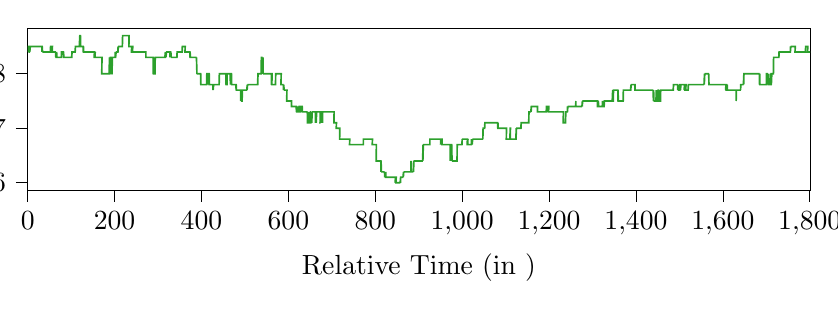
\begin{tikzpicture}[
baseline,
trim axis right,
trim axis left
]

\definecolor{color0}{rgb}{0.172549019607843,0.627450980392157,0.172549019607843}

\begin{axis}[
height=0.3\textwidth,
tick align=outside,
tick pos=left,
width=0.95\textwidth,
x grid style={white!69.0196078431373!black},
xlabel={Relative Time (in \si{\second})},
xmin=0, xmax=1800.934324955,
xtick style={color=black},
y grid style={white!69.0196078431373!black},
ylabel style={align=center},
ylabel={\(\displaystyle \vartheta_{cav}\) (in \si{\celsius})},
ymin=37.58649755, ymax=37.88350745,
ytick style={color=black},
yticklabel pos=lower
]
\addplot [semithick, color0]
table {%
0 37.84
0.599210530002892 37.849998
1.20014349100529 37.849998
0.604668883002887 37.849998
1.20564956500311 37.849998
1.80059134900512 37.849998
1.80488658700051 37.84
2.40015559599851 37.849998
2.4044899090004 37.849998
3.00015635599993 37.849998
3.60002171800443 37.849998
3.00477137100097 37.849998
4.20005537300312 37.849998
3.60468447900348 37.84
4.79933050399995 37.84
4.20570347700414 37.84
5.40010526600236 37.849998
4.80554769300215 37.84
6.00008943400462 37.849998
5.40552414500416 37.849998
6.59969108000223 37.849998
6.00505207000242 37.849998
7.14079292699898 37.849998
6.60490418300469 37.849998
7.2037514170006 37.849998
7.80391753400181 37.849998
7.80614374900324 37.849998
8.4039020880009 37.849998
8.40633957600221 37.849998
9.00389262800309 37.849998
9.60376314400492 37.849998
9.0057103920044 37.849998
9.60589269200136 37.849998
10.2052340110022 37.849998
10.206059119002 37.849998
10.8046210890025 37.849998
10.8060877989992 37.849998
11.3100734440013 37.849998
11.4062680120041 37.849998
12.0061571590049 37.849998
12.1100734440042 37.849998
12.6060552230047 37.849998
13.2015439009992 37.849998
12.606648990004 37.849998
13.2072170710017 37.849998
13.8019237379995 37.849998
14.4029025080017 37.849998
13.8074959950027 37.849998
14.4082051549995 37.849998
15.0032442709999 37.849998
15.0085364330007 37.849998
15.6036267630043 37.849998
15.6083816530008 37.849998
16.2039221470041 37.849998
16.8078352130033 37.849998
16.2094185489987 37.849998
17.4078033469996 37.849998
16.8103711910007 37.849998
17.409710179003 37.849998
18.0093144839993 37.849998
18.6086201380022 37.849998
18.0101490230008 37.849998
19.0790734440016 37.849998
18.6105129190037 37.849998
19.2101270810017 37.849998
19.8063434310025 37.849998
20.406973615005 37.849998
19.8118566330013 37.849998
20.4118007850047 37.849998
21.0076249350022 37.849998
21.6079832169999 37.849998
21.0122718130006 37.849998
21.6127878430052 37.849998
22.0820734439985 37.849998
22.2116834850021 37.849998
22.6800734440039 37.849998
23.4088680120039 37.849998
22.8129082110027 37.849998
23.4148056030026 37.849998
24.009061757999 37.849998
24.6094800819992 37.849998
24.0146682630002 37.849998
24.6154409160008 37.849998
25.2107024350044 37.849998
25.216149576001 37.849998
25.8112068140035 37.849998
25.816120471005 37.849998
26.411631889001 37.849998
26.4163148730004 37.849998
26.9260734440031 37.849998
27.0156238290001 37.849998
27.5270734439982 37.849998
27.6154925480005 37.849998
28.0830734440024 37.849998
28.6850734440013 37.849998
28.2169365770023 37.849998
29.2860734440037 37.849998
28.8174149080005 37.849998
30.0130987900047 37.849998
29.4175243830032 37.849998
30.6133290590005 37.849998
30.0196176030004 37.849998
31.2148164399987 37.849998
30.6187859659985 37.849998
31.2203590339996 37.849998
31.8150027119991 37.849998
32.4152249210019 37.849998
31.8203227470003 37.849998
32.4211072730031 37.849998
33.0157443900025 37.849998
33.0213852540037 37.84
33.5320734440029 37.849998
34.1280734440006 37.84
33.6198015180053 37.84
34.7310734440034 37.84
34.2195266909985 37.84
35.3300734440054 37.84
34.8208756980021 37.84
35.8900734440031 37.84
35.4215349689985 37.84
36.4880734440012 37.84
36.0222553179992 37.84
36.620767694003 37.84
37.2171987710026 37.84
37.2233513860047 37.84
37.8182959650003 37.84
37.8236907200044 37.84
38.4185219400024 37.84
38.4238782910033 37.84
39.0188724399995 37.84
39.0242108509992 37.84
39.6194169220034 37.84
39.6249113020021 37.84
40.2193532640013 37.84
40.2249561880017 37.84
40.6930734440029 37.84
40.8237374000018 37.84
41.4110734440037 37.84
41.9360734440052 37.84
41.4233732180001 37.84
42.5390734440007 37.84
42.0233759930052 37.84
43.094073444001 37.84
42.6250020350053 37.84
43.6970734440038 37.84
43.2249733510034 37.84
44.4207369680007 37.84
43.825325251004 37.84
45.0209981299995 37.84
44.4268745220033 37.84
45.026682335003 37.84
45.6212183969983 37.84
45.6275525930032 37.84
46.2214838069995 37.84
46.2273982510014 37.84
46.8223811210046 37.84
46.8277771409994 37.84
47.4226542219985 37.84
48.0231743390032 37.84
47.4281039929992 37.84
48.623028177004 37.84
48.0280022410006 37.84
48.6282199690031 37.84
49.2234402950053 37.84
49.7020734440011 37.84
49.2288481659998 37.84
49.827638859002 37.84
50.3030734440035 37.84
50.4272700660003 37.84
50.9020734439982 37.84
51.0275100889994 37.84
51.5020734440041 37.84
52.104073444003 37.84
51.6290410760048 37.84
52.2291319270007 37.84
52.7460734440028 37.849998
52.8283755410012 37.849998
53.3010734440031 37.849998
53.4292603130016 37.84
54.0250476910005 37.849998
54.0316643480037 37.84
54.6252546780015 37.84
55.2257521409992 37.849998
54.6308417460023 37.84
55.8268121830042 37.849998
55.2315851849999 37.849998
55.8324019350039 37.849998
56.4270429829994 37.849998
56.9460734439999 37.849998
56.4324164900027 37.84
57.0314908299988 37.84
57.5460734439985 37.84
58.1470734440009 37.84
57.6310261590043 37.84
58.6334739430022 37.84
58.232566769002 37.84
59.3470734440052 37.84
58.8324083530024 37.84
59.4325955169988 37.84
60.028749776 37.84
60.0340433340025 37.84
60.6292060230044 37.84
60.6350512979989 37.84
61.2296616660024 37.84
61.2350940290053 37.84
61.8307592839992 37.84
62.4310725030009 37.84
61.8360820200032 37.84
62.4366364960006 37.84
62.956073444002 37.84
63.034835506005 37.84
63.5090734440018 37.84
63.6347482240017 37.84
64.1510734440017 37.84
64.7100734440028 37.84
64.2365330540051 37.84
64.8369555210011 37.830006
65.3190734439995 37.84
65.4373115679991 37.830006
65.9110734440037 37.830006
66.037279850003 37.830006
66.6328501500029 37.84
67.2331783250047 37.830006
66.6386630179986 37.830006
67.8335072970003 37.830006
67.2387709670002 37.830006
67.8390780090049 37.830006
68.4338660170033 37.830006
69.0345331470016 37.830006
68.440179889003 37.830006
69.0399408060039 37.830006
69.634337028001 37.830006
70.1110734440008 37.830006
69.6404432400013 37.830006
70.7120734440032 37.830006
70.2388546060029 37.830006
71.3130734439983 37.830006
70.8388732009989 37.830006
71.440398358005 37.830006
71.9110734440037 37.830006
72.5540734440001 37.830006
72.0405794640028 37.830006
73.1160734439982 37.830006
72.6409073480027 37.830006
73.8365301750018 37.830006
73.2411517319997 37.830006
74.436824825003 37.830006
73.8428113590053 37.830006
75.0371292230047 37.830006
74.4427672829988 37.830006
75.6375259720007 37.830006
75.0427994560014 37.830006
75.6435990919999 37.830006
76.2386809279997 37.830006
76.2436047400042 37.830006
76.8383764270038 37.830006
76.8446866240047 37.830006
77.3430734440044 37.830006
77.4431468900002 37.830006
77.9210734439985 37.84
78.0426521570043 37.84
78.5210734440043 37.84
78.6440598560002 37.84
79.1670734440049 37.84
79.2445175270041 37.84
79.7690734440039 37.84
79.8449740490032 37.84
80.3220734440038 37.84
80.4447217050038 37.84
81.0405712030042 37.84
81.6408507710003 37.84
81.0460622180035 37.84
81.6466415040049 37.84
82.2414109710007 37.84
82.2466721329984 37.830006
82.8415584300019 37.84
82.847331115001 37.830006
83.4426179540023 37.830006
83.4479355580042 37.830006
84.0422008110036 37.830006
84.048101846005 37.830006
84.5270734439982 37.830006
84.6465194289995 37.830006
85.1490734440013 37.830006
85.7720734440009 37.830006
85.2465458600054 37.830006
86.3720734439994 37.830006
85.8480704180038 37.830006
86.9260734440031 37.830006
86.4485647760011 37.830006
87.5710734439999 37.830006
87.0479952940004 37.830006
87.649298426004 37.830006
88.2446972700054 37.830006
88.8449801410025 37.830006
88.2505845090054 37.830006
89.446025160003 37.830006
88.8511870840011 37.830006
90.0457654380007 37.830006
89.4515523630034 37.830006
90.6462801450034 37.830006
90.0516401749992 37.830006
90.6524846629982 37.830006
91.1350734439984 37.830006
91.7770734439982 37.830006
91.2509902640013 37.830006
92.3810734440049 37.830006
91.8509157740045 37.830006
92.4518319999988 37.830006
92.9370734440017 37.830006
93.5340734440033 37.830006
93.0524682360046 37.830006
93.6528090300053 37.830006
94.2481619020036 37.830006
94.2536493200023 37.830006
94.8484927040045 37.830006
94.8537923580006 37.830006
95.4487492769986 37.830006
96.0490496249986 37.830006
95.4558504540037 37.830006
96.0557863360009 37.830006
96.6490994830019 37.830006
96.6544949610034 37.830006
97.2497049390004 37.830006
97.2555818820038 37.830006
97.8499588560007 37.830006
97.8560175150051 37.830006
98.4510696650032 37.830006
98.451083164 37.830006
98.9360734440052 37.830006
99.0545787779993 37.830006
99.5360734440037 37.830006
99.6544674129982 37.830006
100.143073444 37.830006
100.739073444005 37.830006
100.256431300004 37.830006
100.856372991999 37.830006
101.382073444001 37.830006
102.05199647 37.84
101.455579052999 37.830006
102.057386 37.84
102.652490697001 37.84
102.657574399003 37.84
103.252445704005 37.84
103.258274737003 37.84
103.852877047 37.84
103.858465017001 37.84
104.453079872001 37.84
104.459544998004 37.84
105.053542456 37.84
105.059250696999 37.84
105.654445161999 37.84
105.659773247004 37.84
106.192073443999 37.84
106.258770291999 37.84
106.749073444 37.84
107.349073443998 37.84
106.858804692005 37.84
107.458755789004 37.84
107.950073444001 37.84
108.060142171998 37.84
108.551073444003 37.84
108.660705225004 37.84
109.255663241005 37.84
109.856002527005 37.849998
109.261143376003 37.84
109.861321285003 37.849998
110.456340058001 37.849998
110.461770735004 37.849998
111.056629543004 37.849998
111.657057827004 37.849998
111.061961763 37.849998
112.258093584998 37.849998
111.663506440003 37.849998
112.858439124 37.849998
112.263531271004 37.849998
113.356073444003 37.849998
112.863793091004 37.849998
113.959073443999 37.849998
113.462317411002 37.849998
114.560073444001 37.849998
114.062036563999 37.849998
115.143073444 37.849998
114.663761344003 37.849998
115.859702984002 37.849998
115.263230805998 37.849998
115.865013310999 37.849998
116.460008644004 37.849998
117.060377040005 37.849998
116.465416128005 37.849998
117.660798736004 37.849998
117.065783180005 37.849998
118.261346633 37.849998
117.666334402005 37.849998
118.714073444004 37.849998
118.261357378004 37.849998
119.318073444003 37.849998
118.861813214004 37.849998
120.011073444002 37.870007
119.466523996001 37.849998
120.066438900001 37.870007
120.570073444003 37.870007
120.667335966005 37.870007
121.144073444004 37.870007
121.267740019 37.849998
121.771073444004 37.870007
121.868280668001 37.849998
122.413073444004 37.849998
122.463848672 37.849998
122.969073444001 37.849998
123.064252279 37.849998
123.569073444 37.849998
123.664532134004 37.849998
124.229073444003 37.849998
124.264880152004 37.849998
124.770073444 37.849998
124.865301967002 37.849998
125.372073443999 37.849998
125.465643736999 37.849998
125.971073444001 37.849998
126.069935173 37.849998
126.615073444002 37.849998
126.669795601003 37.849998
127.220073444005 37.849998
127.271690414003 37.849998
127.723073444002 37.849998
127.871959741002 37.84
128.421073443998 37.849998
128.467506131004 37.84
128.976073443999 37.84
129.067685198999 37.84
129.625073444004 37.84
129.668284113002 37.84
130.148073444005 37.84
130.268574564005 37.84
130.781073443999 37.84
130.868692418 37.84
131.329073444002 37.84
131.468954930002 37.84
131.981073444003 37.84
132.069282005003 37.84
132.626073444 37.84
132.670151750004 37.84
133.182073444004 37.84
133.274423046001 37.84
133.782073444003 37.84
133.874304814002 37.84
134.381073444005 37.84
134.475411960004 37.84
135.027073443998 37.84
135.075728511001 37.84
135.583073444002 37.84
135.675949534001 37.84
136.183073444001 37.84
136.276086049002 37.84
136.783073443999 37.84
136.876503289001 37.84
137.382073444001 37.84
137.476797341005 37.84
137.984073444 37.84
138.071931031998 37.84
138.585073444003 37.84
138.671952666002 37.84
139.185073444001 37.84
139.272286076004 37.84
139.872491728005 37.84
139.878671099999 37.84
140.472685145003 37.84
140.478752530005 37.84
141.072895744001 37.84
141.078688852002 37.84
141.673098161998 37.84
141.679055239001 37.84
142.273352057004 37.84
142.278979338 37.84
142.786073444004 37.84
142.877791022001 37.84
143.280076135001 37.84
143.477643505001 37.84
143.987073444005 37.84
144.077710825004 37.84
144.588073444 37.84
144.677643037001 37.84
145.187073444002 37.84
145.279379369 37.84
145.788073444004 37.84
145.879600988999 37.84
146.388073444003 37.84
146.479025109998 37.84
146.989073444005 37.84
147.079999426998 37.84
147.589073444004 37.84
147.680532478 37.84
148.275914768004 37.84
148.281134165001 37.84
148.876233003 37.84
148.882914595 37.84
149.476549352999 37.84
149.481906524001 37.84
150.076604309004 37.84
150.082142008003 37.84
150.677131935001 37.84
150.683679189999 37.84
151.277178346005 37.84
151.283139491999 37.84
151.795073444002 37.84
152.395073444 37.84
151.881561006005 37.84
152.996073444003 37.84
152.481575204001 37.84
153.596073444001 37.84
153.083082499004 37.830006
154.197073444004 37.830006
153.683311318004 37.830006
154.797073444002 37.84
154.283781413003 37.830006
155.479425491001 37.84
154.883993515003 37.830006
156.079912791 37.830006
155.484735796999 37.830006
156.680099862002 37.830006
156.085153812004 37.830006
157.280513507001 37.830006
156.685605938001 37.830006
157.880719635003 37.830006
157.285967882002 37.830006
158.481056267003 37.830006
157.886284366003 37.830006
159.003073444001 37.830006
158.486657246001 37.830006
159.602073444003 37.830006
159.085420743002 37.830006
160.216073444004 37.830006
159.685427421005 37.830006
160.804073444 37.830006
160.285912520005 37.830006
161.406073443999 37.830006
160.887669456002 37.830006
161.487500169998 37.830006
162.082887274999 37.830006
162.088971782003 37.830006
162.683127891003 37.830006
162.688370240001 37.830006
163.283514891998 37.830006
163.288768885002 37.830006
163.883780159005 37.830006
163.889246929 37.830006
164.484112470003 37.830006
164.489527209 37.830006
165.084498340999 37.830006
165.089778316004 37.830006
165.684723273 37.830006
165.690353495003 37.830006
166.285063690004 37.830006
166.291071710002 37.830006
166.812073444002 37.830006
166.889891621999 37.830006
167.412073444 37.830006
167.490006956999 37.830006
168.015073444003 37.830006
168.09013389 37.830006
168.617073444002 37.830006
168.692719798004 37.830006
169.286870831005 37.830006
169.292152237002 37.830006
169.887222365003 37.830006
170.487581746005 37.830006
169.892532969003 37.830006
171.087827846 37.830006
170.492778309002 37.799999
171.093155325005 37.799999
171.688248897 37.799999
172.288547001001 37.799999
171.693876344005 37.799999
172.293848918001 37.799999
172.888804545 37.799999
172.894426252999 37.799999
173.416073444001 37.799999
174.019073444004 37.799999
173.493567704005 37.799999
174.093757303999 37.799999
174.619073444002 37.799999
174.693349093002 37.799999
175.216073444004 37.799999
175.816073444003 37.799999
175.294839510003 37.799999
176.424073444003 37.799999
175.895174896003 37.799999
176.494467456003 37.799999
177.090956359003 37.799999
177.691896909004 37.799999
177.096242781001 37.799999
177.696537290001 37.799999
178.291580771001 37.799999
178.891736799 37.799999
178.296705339002 37.799999
178.897029051004 37.799999
179.491924351001 37.799999
179.497356803004 37.799999
180.092613427005 37.799999
180.692614767002 37.799999
180.098852599003 37.799999
181.238073444001 37.799999
180.698058915004 37.799999
181.830073444005 37.799999
181.297307332003 37.799999
181.897623353005 37.799999
182.428073444004 37.799999
183.031073443999 37.799999
182.497625231001 37.799999
183.098884693005 37.799999
183.632073444001 37.799999
184.235073444004 37.799999
183.699181778 37.799999
184.836073443999 37.799999
184.299641165999 37.799999
184.899652092005 37.799999
185.437073444002 37.799999
186.095656554004 37.799999
185.500219476002 37.799999
186.100870678005 37.799999
186.695918001999 37.799999
186.701397763005 37.799999
187.296392852004 37.799999
187.896605740003 37.799999
187.301707365004 37.799999
188.439073444002 37.830006
187.902659788 37.799999
189.037073444 37.830006
188.501796821001 37.830006
189.670890819005 37.830006
189.101515766 37.799999
190.242073444002 37.799999
189.700971188999 37.799999
190.842073444001 37.799999
190.302733390003 37.799999
191.499093260005 37.830006
190.902844451004 37.799999
191.504326396003 37.830006
192.098613466005 37.830006
192.103831058004 37.799999
192.698758908999 37.830006
193.299169966005 37.799999
192.704032364003 37.799999
193.305323749999 37.799999
193.900061758999 37.799999
194.500378069999 37.830006
193.904636749001 37.799999
195.099893808001 37.830006
194.505080391005 37.830006
195.105276437003 37.830006
195.700128249999 37.830006
196.300366020005 37.830006
195.705404560002 37.830006
196.305702831 37.830006
196.900611602003 37.830006
197.353073443999 37.830006
196.906940141002 37.830006
197.957073443999 37.830006
197.504832203005 37.830006
198.105361779999 37.830006
198.557073444004 37.830006
198.705175872004 37.830006
199.199073444004 37.830006
199.307007879004 37.830006
199.758073444005 37.830006
199.906039633999 37.830006
200.355073444 37.830006
200.956073444002 37.830006
200.506980896003 37.830006
201.107096211002 37.830006
201.702538821002 37.84
201.708787493 37.830006
202.302806420004 37.830006
202.903058675998 37.84
202.308153044003 37.830006
203.503438004998 37.84
202.908527079999 37.84
204.103815975999 37.84
203.508767068 37.84
204.704074699999 37.84
204.109207103 37.84
205.304444246001 37.84
204.709371142999 37.84
205.763073444003 37.84
205.309746596999 37.84
206.362073444005 37.84
205.908697453 37.84
206.963073444 37.84
206.508690248003 37.84
207.109420911002 37.84
207.564073444002 37.84
208.164073444001 37.849998
207.711017226 37.84
208.764073443999 37.849998
208.310567458 37.849998
209.507154674 37.849998
208.910161204003 37.849998
210.106720324999 37.849998
209.512581852003 37.849998
210.112648640003 37.849998
210.707067625 37.849998
211.308251428003 37.849998
210.712374451003 37.849998
211.313059986001 37.849998
211.907776143002 37.849998
212.508232573004 37.849998
211.913147817002 37.849998
213.108427918 37.849998
212.513709980005 37.849998
213.570073444003 37.849998
213.114638872001 37.849998
214.255073444001 37.849998
213.712511432001 37.849998
214.814073444002 37.849998
214.315014871005 37.849998
214.915324159003 37.849998
215.414073444001 37.849998
215.514597068002 37.849998
215.973073444002 37.849998
216.115046461004 37.849998
216.710327790002 37.849998
216.717171822005 37.849998
217.311483022 37.849998
217.316879351005 37.849998
217.910957372005 37.849998
217.916662073003 37.849998
218.511115991001 37.870007
218.516402542002 37.870007
219.112481159005 37.870007
219.117981821 37.870007
219.712439587005 37.870007
219.718097466 37.870007
220.312904617 37.870007
220.91232974 37.870007
220.317333257 37.870007
220.917872585 37.870007
221.512376756 37.870007
221.517785182004 37.870007
222.018073444 37.870007
222.619073444002 37.870007
222.117322131999 37.870007
223.273073444005 37.870007
222.716604453002 37.870007
223.823073444 37.870007
223.316856973004 37.870007
224.428073444004 37.870007
223.919257852001 37.870007
224.518081204005 37.870007
225.023073444005 37.870007
225.581073444002 37.870007
225.119257081999 37.870007
226.183073444001 37.870007
225.718580200002 37.870007
226.822073444004 37.870007
226.318653091999 37.870007
227.515532685 37.870007
226.918917770003 37.870007
228.114928218005 37.870007
227.520777634003 37.870007
228.120421716005 37.870007
228.715096644002 37.870007
228.720404801003 37.870007
229.316384862002 37.870007
229.915604608002 37.870007
229.321675753003 37.870007
230.515887134003 37.870007
229.922081811004 37.870007
230.522328265004 37.870007
231.115971979001 37.870007
231.589073444004 37.870007
231.121391715998 37.870007
232.320503631003 37.870007
231.720901549001 37.870007
232.323129825003 37.870007
232.792073444005 37.870007
233.428073444004 37.870007
232.921838341004 37.849998
233.993073443999 37.849998
233.522050676002 37.849998
234.628073444001 37.849998
234.122379123 37.849998
234.723479403001 37.849998
235.319220256002 37.849998
235.323554622999 37.849998
235.918974762004 37.849998
235.924302865002 37.849998
236.519079205005 37.849998
237.120396413004 37.849998
236.525298510001 37.849998
237.124637271001 37.849998
237.719691793005 37.849998
237.725305316999 37.849998
238.320027993999 37.849998
238.325376604 37.849998
238.799073444003 37.849998
239.399073444001 37.849998
238.924745215001 37.84
239.999073444 37.84
239.524841530001 37.84
240.600073444002 37.84
240.126438093001 37.84
240.726342351001 37.84
241.237073444005 37.849998
241.834073443999 37.849998
241.325995879 37.84
242.404073443999 37.84
241.926366312 37.84
243.121840054002 37.84
242.526537415004 37.84
243.723160316003 37.84
243.128016477 37.84
244.323447139999 37.84
243.727582967003 37.84
244.922657175004 37.84
244.328734173003 37.84
245.523122760002 37.84
244.929020674004 37.84
246.123184476004 37.84
245.528651355002 37.84
246.723329594999 37.84
246.129497219001 37.84
247.323581346005 37.84
246.729583556 37.84
247.329013488001 37.84
247.924513010999 37.84
247.928970705005 37.84
248.524569493005 37.84
248.529286632998 37.84
249.123880163999 37.84
249.729164848999 37.84
249.129637623999 37.84
250.328420278005 37.84
249.729931536 37.84
250.330041214998 37.84
250.930011683005 37.84
251.530281965999 37.84
251.128656198001 37.84
251.728187786 37.84
252.128325313999 37.84
252.130959996 37.84
252.729360005003 37.84
253.330490756001 37.84
252.731486870005 37.84
253.931274022005 37.84
253.332017200999 37.84
254.531482445003 37.84
254.048073443999 37.84
254.654073443999 37.84
255.130915435999 37.84
255.732075582004 37.84
255.197073444004 37.84
255.851073443999 37.84
256.331120011004 37.84
256.386073444002 37.84
256.932119885001 37.84
257.531537993003 37.84
257.051073444003 37.84
258.131950881005 37.84
257.655073444002 37.84
258.732673707003 37.84
258.257073444001 37.84
259.332976500998 37.84
258.821073444 37.84
259.932992080001 37.84
259.456073444002 37.84
260.061073444005 37.84
260.532121525001 37.84
261.132291763002 37.84
260.656073443999 37.84
261.733324346998 37.84
261.222073444005 37.84
261.821073444 37.84
262.332638190004 37.84
262.460073444003 37.84
262.933515952005 37.84
263.064073444002 37.84
263.532814871003 37.84
264.133131497001 37.84
263.623073444003 37.84
264.224073443998 37.84
264.733212607003 37.84
264.865073444002 37.84
265.333622677004 37.84
265.933662283998 37.84
265.425073443999 37.84
266.534171517 37.84
266.068073444003 37.84
267.133810804 37.84
266.664073444001 37.84
267.269073444004 37.84
267.735037273 37.84
268.334870138002 37.84
267.830073444005 37.84
268.935003223 37.84
268.467073444001 37.84
269.535482842999 37.84
269.068073444003 37.84
269.631073444005 37.84
270.134753580998 37.84
270.734719100001 37.84
270.268073444 37.84
271.335391035005 37.84
270.868073443999 37.84
271.433073444001 37.84
271.935051918001 37.84
271.998341039005 37.830006
272.535130299999 37.830006
272.676073444003 37.830006
273.135481042002 37.830006
273.736205146 37.830006
273.235073444004 37.830006
273.873073444003 37.830006
274.335438521004 37.830006
274.936730364003 37.830006
274.436073444005 37.830006
275.535752856005 37.830006
275.072073444004 37.830006
276.13684608 37.830006
275.672073444002 37.830006
276.218073444004 37.830006
276.737151491005 37.830006
276.875073444004 37.830006
277.336438283004 37.830006
277.937793317004 37.830006
277.382073444001 37.830006
278.536370459005 37.830006
278.038073444004 37.830006
279.136919755001 37.830006
278.676073444003 37.830006
279.241073444005 37.830006
279.737328688003 37.830006
280.337585934001 37.830006
279.876073444 37.830006
280.937997781002 37.830006
280.477073444003 37.830006
281.537590209002 37.830006
281.041073444001 37.830006
281.675073443999 37.830006
282.138263594003 37.830006
282.182073444004 37.830006
282.737644184002 37.830006
282.846073444001 37.830006
283.337606907 37.830006
283.447073444004 37.830006
283.937758826003 37.830006
283.985073444004 37.830006
284.539445854003 37.830006
284.586073443999 37.830006
285.138281983003 37.830006
285.240073444002 37.830006
285.739569853999 37.830006
285.784073444003 37.830006
286.339742855002 37.830006
286.386073444002 37.830006
286.938549012004 37.830006
286.985073444004 37.830006
287.539095493004 37.830006
287.586073443999 37.830006
288.138659715005 37.830006
288.184073444005 37.830006
288.739785127 37.830006
288.856073444003 37.799999
289.339666979002 37.830006
289.487073444005 37.799999
289.939785092 37.799999
290.058073444001 37.799999
290.539820837999 37.799999
290.660073444 37.799999
291.139419505998 37.799999
291.259073444002 37.799999
291.739920805005 37.799999
291.859073444 37.799999
292.339587441005 37.799999
292.940086979004 37.799999
292.487073444005 37.799999
292.992073444002 37.799999
293.539530644004 37.830006
294.139540703 37.830006
293.688073443998 37.830006
294.295073444002 37.830006
294.739657115002 37.830006
295.339735157002 37.830006
294.793073444001 37.830006
295.467073444001 37.830006
295.940430786999 37.830006
296.541100728005 37.830006
296.094073444001 37.830006
297.139854304005 37.830006
296.734427919 37.830006
297.740271192 37.830006
297.296073443998 37.830006
297.895073444 37.830006
298.350073444002 37.830006
298.939906625004 37.830006
298.474073443998 37.830006
299.540036004 37.830006
299.074073444004 37.830006
299.673073443999 37.830006
300.140629762005 37.830006
300.193073444003 37.830006
300.740020734003 37.830006
301.340766257003 37.830006
300.796073443998 37.830006
301.940952271005 37.830006
301.395073444 37.830006
301.996073444003 37.830006
302.540515499 37.830006
302.583073444002 37.830006
303.141276337003 37.830006
303.741885619005 37.830006
303.198073444 37.830006
304.341930577 37.830006
303.882073444001 37.830006
304.942209754001 37.830006
304.399073444001 37.830006
304.984073444 37.830006
305.541354165005 37.830006
306.142176551999 37.830006
305.599073443998 37.830006
306.741990763003 37.830006
306.199073444004 37.830006
306.842073444001 37.830006
307.344407772005 37.830006
307.388073444003 37.830006
307.94334826 37.830006
308.543102834003 37.830006
308.047073444002 37.830006
309.142899842001 37.830006
308.646073444004 37.830006
309.202073444001 37.830006
309.742787977004 37.830006
310.343811289 37.830006
309.794073444005 37.830006
310.944213788003 37.830006
310.404073443999 37.830006
311.543748835 37.830006
311.008073444005 37.830006
312.144680885001 37.830006
311.638073444003 37.830006
312.745089976001 37.830006
312.196073444 37.830006
313.345256339999 37.830006
312.795073444002 37.830006
313.945650498004 37.830006
313.395073444 37.830006
314.544918671003 37.830006
313.996073444003 37.830006
315.145409853001 37.830006
314.597073444005 37.830006
315.746817125 37.830006
315.199073444004 37.830006
316.346574607 37.830006
315.844073444001 37.830006
316.946146348004 37.84
316.457073443999 37.830006
317.546836845002 37.830006
316.999611940999 37.830006
318.147059506002 37.830006
317.611073444001 37.830006
318.747390675002 37.84
318.246073444003 37.830006
319.347915040998 37.84
318.859073444 37.84
319.403073444002 37.84
319.948000276003 37.84
320.547867497 37.84
320.046073443998 37.84
321.148602601002 37.84
320.648073444005 37.84
321.748926208005 37.84
321.262073443999 37.84
322.349376572005 37.84
321.804073444 37.84
322.424073444003 37.84
322.949296636005 37.84
323.022073444001 37.84
323.549507677999 37.84
323.609073444 37.84
324.149694723004 37.84
324.223073444002 37.84
324.750612510004 37.84
324.812073444002 37.84
325.350695305002 37.84
325.466073444004 37.84
325.950479220999 37.84
326.550821517005 37.84
326.013073444003 37.84
327.151079952004 37.84
326.670073444002 37.84
327.751641616 37.84
327.230073444 37.830006
328.352112288005 37.84
327.770907466998 37.84
328.430073444004 37.84
328.952185599002 37.84
329.015073444003 37.830006
329.551827373005 37.84
330.152838881004 37.830006
329.675073443999 37.830006
330.753152060999 37.830006
330.262073443999 37.830006
331.353224731 37.830006
330.858073444004 37.830006
331.952774096004 37.830006
331.484073444 37.830006
332.552736030004 37.830006
332.043073444001 37.830006
333.153080308999 37.830006
332.662073444 37.830006
333.753414327002 37.830006
333.263073444003 37.830006
334.353939660999 37.830006
333.820073444003 37.830006
334.953910194999 37.830006
334.440073443999 37.830006
335.553874509002 37.830006
335.088073444 37.830006
336.154403831002 37.830006
335.667073444005 37.830006
336.754917659004 37.830006
336.229073444003 37.830006
337.354237865999 37.830006
336.888073444003 37.830006
337.955376897 37.830006
337.468073444004 37.830006
338.555038658 37.830006
338.043073444001 37.830006
339.154763908002 37.830006
338.689073444002 37.830006
339.755379603004 37.830006
339.291073444001 37.830006
340.355554624002 37.830006
339.847073444005 37.830006
340.955462506005 37.830006
340.470073444005 37.830006
341.555841351001 37.830006
341.047073444002 37.830006
342.155886706001 37.830006
341.647073444001 37.830006
342.756024887 37.830006
342.230073444 37.830006
343.356880922998 37.830006
342.893073444 37.830006
343.496073444003 37.830006
343.956679278999 37.84
344.556497180005 37.84
344.049073444003 37.84
345.157006448004 37.84
344.679073444 37.84
345.256073444005 37.84
345.757233830998 37.84
345.954531898999 37.84
346.358201353003 37.84
346.957430372 37.84
346.438073443998 37.84
347.557388100002 37.84
347.095073444005 37.84
348.157830206001 37.84
347.638073444003 37.84
348.235073444004 37.84
348.757812929005 37.84
348.850073444002 37.84
349.358038167004 37.84
349.454073444002 37.84
349.957402541004 37.84
350.054073444 37.84
350.557541344999 37.84
350.654073443999 37.84
351.158324921002 37.84
351.758886996999 37.84
351.243073443999 37.84
352.358205582001 37.84
351.855073444 37.84
352.958315511001 37.84
352.404073443999 37.84
353.559002510003 37.84
353.004073444004 37.84
354.158444893001 37.84
353.700073444001 37.84
354.758815226 37.84
354.256073444005 37.84
355.358889571005 37.84
354.859073444 37.84
355.552903087999 37.84
355.958612882001 37.849998
356.006073444005 37.849998
356.558635324 37.849998
356.692073443999 37.849998
357.159412330999 37.849998
357.241073444005 37.849998
357.759659221003 37.849998
357.808073444001 37.849998
358.359986486001 37.849998
358.460073444003 37.849998
358.959957481005 37.849998
359.009073444002 37.849998
359.559590833 37.849998
359.651073444002 37.849998
360.160285671001 37.849998
360.295073444002 37.849998
360.760243563003 37.849998
361.360616256003 37.849998
360.897073444001 37.849998
361.960487646 37.849998
361.558695856002 37.849998
362.560597674004 37.849998
362.109073444 37.84
363.161036030004 37.84
362.662073444 37.84
363.760991376002 37.84
363.244073444002 37.84
364.360334791003 37.84
363.867073444002 37.84
364.961247257001 37.84
364.503073444001 37.84
365.560947513004 37.84
365.059073444005 37.84
366.161487039004 37.84
365.615073444002 37.84
366.761724329001 37.84
366.267073444003 37.84
367.362007618001 37.84
366.868073443999 37.84
367.962220746005 37.84
367.466073444004 37.84
368.561281890004 37.84
368.112073444005 37.84
368.664073444001 37.84
369.162383688003 37.84
369.244073444002 37.84
369.762346077005 37.84
369.865073444002 37.84
370.361663053001 37.84
370.468073444004 37.84
370.962461023002 37.84
371.014073443999 37.84
371.562665739002 37.84
371.666073444001 37.84
372.162557117001 37.84
372.220073444005 37.84
372.762538536001 37.84
372.819073444 37.84
373.362935516001 37.84
373.415073444005 37.830006
373.962938110999 37.84
374.071073444 37.830006
374.562901636004 37.830006
374.671073443998 37.830006
375.162745112 37.830006
375.216073444004 37.830006
375.763101461001 37.830006
375.816073444003 37.830006
376.363087350001 37.830006
376.515073444003 37.830006
376.963142355999 37.830006
377.071073444 37.830006
377.563147387998 37.830006
377.675073443999 37.830006
378.163273857004 37.830006
378.252073444004 37.830006
378.763220509005 37.830006
378.876073444 37.830006
379.363268820001 37.830006
379.519073444004 37.830006
379.963416359999 37.830006
380.562781076005 37.830006
380.023073444005 37.830006
381.163400598001 37.830006
380.724073443998 37.830006
381.763729361999 37.830006
381.276073444002 37.830006
382.363669488004 37.830006
381.878073444001 37.830006
382.963747597001 37.830006
382.479073444003 37.830006
383.563763835999 37.830006
383.024073444001 37.830006
384.163651178998 37.830006
383.723073444002 37.830006
384.764003845004 37.830006
384.229073444003 37.830006
385.364160982004 37.830006
384.883073444005 37.830006
385.964200977003 37.830006
385.530073444002 37.830006
386.563793214998 37.830006
386.085073444003 37.830006
387.164370589002 37.830006
386.687073444002 37.830006
387.764835314003 37.830006
387.289073444001 37.830006
388.364390808005 37.830006
387.888073444003 37.830006
388.964528665005 37.830006
388.485073444004 37.830006
389.565108077004 37.799999
389.129359295002 37.799999
390.165306473005 37.799999
389.731073444003 37.799999
390.7643685 37.799999
390.276073444002 37.799999
391.364740088 37.799999
390.887073443999 37.799999
391.965203947002 37.799999
391.532073444003 37.799999
392.565228217005 37.799999
392.088073444 37.799999
392.689073444002 37.799999
393.165292123005 37.799999
393.290073444005 37.799999
393.765535067003 37.799999
393.892073444003 37.799999
394.366183038001 37.799999
394.435073444001 37.799999
394.966242130002 37.799999
395.136073444002 37.799999
395.566475198 37.799999
395.639073443999 37.799999
396.167205543999 37.799999
396.257073444001 37.799999
396.767830279001 37.799999
396.835073444003 37.799999
397.367484284005 37.799999
397.492073444002 37.799999
397.967604506004 37.799999
398.092073444001 37.779991
398.567572616004 37.799999
398.694073444 37.779991
399.168219496001 37.779991
399.295073444002 37.779991
399.768925281001 37.779991
399.895073444 37.779991
400.369047483 37.779991
400.496073444003 37.779991
400.968816262 37.779991
401.096073444001 37.779991
401.568891272 37.779991
401.695073444003 37.779991
402.169052299003 37.779991
402.295073444002 37.779991
402.770304631005 37.779991
402.896073444004 37.779991
403.370708212002 37.779991
403.495073443999 37.779991
403.970796874004 37.779991
404.096073444001 37.779991
404.570300468004 37.779991
404.700073444001 37.779991
405.171203269005 37.779991
405.265073444003 37.779991
405.771439092001 37.779991
405.903073444002 37.779991
406.371764285999 37.779991
406.503073444001 37.779991
406.972049344004 37.779991
407.103073443999 37.779991
407.572757362002 37.779991
407.703073444005 37.779991
408.172160003 37.779991
408.304073444 37.779991
408.773236150999 37.779991
408.906073443999 37.779991
409.373673686001 37.779991
409.506073444005 37.779991
409.973936362003 37.779991
410.106073444003 37.779991
410.572967395005 37.779991
410.711073443999 37.779991
411.173610903003 37.779991
411.271073444004 37.779991
411.773471938002 37.779991
411.817073443999 37.779991
412.372814981005 37.799999
412.417073444005 37.799999
412.980894660999 37.799999
413.108073444004 37.799999
413.573008905005 37.799999
413.622073443999 37.779991
414.173156239005 37.799999
414.217073444001 37.779991
414.773460028999 37.799999
414.826073444005 37.799999
415.372781894002 37.799999
415.424073444003 37.799999
415.972887447999 37.799999
416.023073444005 37.799999
416.572882859 37.799999
416.620073443999 37.799999
417.210419708004 37.799999
417.252073444004 37.779991
417.773503272001 37.799999
417.823073444 37.779991
418.372881759999 37.779991
418.972779610005 37.779991
418.428073444004 37.779991
419.616073444005 37.779991
419.027073443998 37.779991
420.172750087004 37.779991
419.767406853003 37.779991
420.817073443999 37.779991
420.225073444002 37.779991
421.372560053998 37.779991
420.967640991999 37.779991
421.973687837999 37.779991
421.427073444 37.779991
422.573005080005 37.779991
422.027073443998 37.779991
423.217073444001 37.779991
422.631073444005 37.779991
423.772291088004 37.779991
423.280073444002 37.779991
424.372581118005 37.779991
423.835073444003 37.779991
424.972338236999 37.779991
424.566771853002 37.779991
425.619073444002 37.779991
425.030073444002 37.779991
426.172814893005 37.779991
425.766789310001 37.779991
426.772305929 37.779991
426.231073444003 37.769997
427.399756162005 37.779991
426.832073443999 37.769997
427.972165251005 37.779991
427.440073443999 37.779991
428.573109050005 37.779991
428.036073444004 37.779991
429.171603670999 37.779991
428.639073443999 37.779991
429.772260160003 37.779991
429.238073444001 37.779991
430.372056551001 37.779991
429.839073444004 37.779991
430.972316251005 37.779991
430.443073444003 37.779991
431.572062769999 37.779991
431.024073444001 37.779991
432.172163000003 37.779991
431.625073444004 37.779991
432.771859474 37.779991
432.243073443999 37.779991
433.37262953 37.779991
432.842073444001 37.779991
433.427073444 37.779991
433.971995418004 37.779991
434.047073444002 37.779991
434.572068002002 37.779991
434.646073444004 37.779991
435.172035740005 37.779991
435.246073444003 37.779991
435.771842932001 37.779991
435.831073444002 37.779991
436.371835479003 37.779991
436.432073444004 37.779991
436.972332299003 37.779991
437.047073444002 37.779991
437.572187185004 37.779991
437.650073444005 37.779991
438.172484727002 37.779991
438.234073444 37.779991
438.772558281002 37.779991
438.836073443999 37.779991
439.371772261999 37.779991
439.435073444001 37.779991
439.972161669 37.779991
440.051073444003 37.779991
440.571419347005 37.779991
440.651073444002 37.779991
441.171399611005 37.799999
441.236073444001 37.799999
441.771950886003 37.799999
441.837073444003 37.799999
442.371325124004 37.799999
442.439073444002 37.799999
442.971393275002 37.799999
443.051073444003 37.799999
443.571224218002 37.799999
443.655073444002 37.799999
444.171288234 37.799999
444.252073444004 37.799999
444.771195314999 37.799999
444.855073444 37.799999
445.371440966999 37.799999
445.443073444003 37.799999
445.970635293001 37.799999
446.042073444005 37.799999
446.570399465003 37.799999
446.655073444002 37.799999
447.170244676003 37.799999
447.244073444002 37.799999
447.770586046005 37.799999
447.858073444004 37.799999
448.370163222004 37.799999
448.454073444002 37.799999
448.970508634004 37.799999
449.058073444001 37.799999
449.569955076004 37.799999
449.655073444002 37.799999
450.169652121003 37.799999
450.251073444 37.799999
450.770490392002 37.799999
450.858073444004 37.799999
451.369628894005 37.799999
451.458073444002 37.799999
451.969801753003 37.799999
452.054073444 37.799999
452.569540130004 37.799999
452.651073444002 37.799999
453.169481443001 37.799999
453.258073444005 37.799999
453.769648308 37.799999
453.858073444004 37.799999
454.369748595003 37.799999
454.458073444002 37.799999
454.970202597004 37.799999
455.054073444 37.799999
455.569445646004 37.799999
455.658073443999 37.799999
456.170510655 37.799999
456.262073443999 37.779991
456.770684360999 37.799999
456.866073444005 37.779991
457.370572858999 37.779991
457.455073444005 37.779991
457.970676244004 37.779991
458.062073444002 37.779991
458.570204050004 37.779991
458.666073444001 37.779991
459.170720524999 37.799999
459.239073444005 37.799999
459.769907318005 37.799999
459.866073444005 37.799999
460.370468708999 37.799999
460.459073443999 37.799999
460.970479624004 37.799999
461.067073443999 37.799999
461.571101639005 37.799999
461.661073444004 37.799999
462.235073444004 37.799999
462.368791141998 37.799999
462.771408689005 37.799999
462.866073444005 37.799999
463.370891514001 37.799999
463.467073444001 37.799999
463.971092393003 37.799999
464.075073444001 37.799999
464.570330697999 37.799999
464.670073444002 37.799999
465.170832283999 37.799999
465.271073444004 37.799999
465.770940925999 37.799999
465.873073444003 37.799999
466.370971927005 37.799999
466.449004362999 37.779991
466.970912936005 37.799999
467.075073444001 37.799999
467.570806071999 37.799999
467.675073443999 37.799999
468.180358329999 37.799999
468.278073444002 37.799999
468.770199307 37.799999
468.878073444001 37.779991
469.370834658002 37.799999
469.488073444001 37.779991
469.969879802004 37.779991
470.082073443999 37.779991
470.569712707998 37.779991
470.679073444 37.779991
471.170776965999 37.779991
471.283073443999 37.779991
471.770393522005 37.779991
471.888073444003 37.779991
472.370003573 37.779991
472.478073443999 37.779991
472.969516322002 37.779991
473.083073444002 37.779991
473.569268038002 37.779991
473.679073444 37.779991
474.235073444004 37.779991
474.287073444 37.779991
474.769068665999 37.779991
474.897073444001 37.779991
475.368718064004 37.779991
475.491073444005 37.779991
475.968662008003 37.779991
476.091073444004 37.779991
476.568491303005 37.779991
476.692073443999 37.779991
477.168291212001 37.779991
477.294073444005 37.779991
477.768257651005 37.779991
477.896073444004 37.779991
478.368111948002 37.779991
478.490073444002 37.779991
478.967858595999 37.779991
479.082073443999 37.779991
479.567837210001 37.779991
479.696073444 37.769997
480.167583220005 37.779991
480.275073444005 37.769997
480.767558140004 37.769997
480.895073444 37.769997
481.367335802999 37.769997
481.499073444 37.769997
481.967602868004 37.769997
482.100073444002 37.769997
482.567620016998 37.769997
482.761946416998 37.769997
483.167296174004 37.769997
483.300073443999 37.769997
483.767903843 37.769997
483.961941589005 37.769997
484.367516286999 37.769997
484.500073444004 37.769997
484.966628836999 37.769997
485.088073444 37.769997
485.566699170005 37.769997
485.690073443999 37.769997
486.209073443999 37.769997
486.264073443999 37.769997
486.767040938001 37.769997
486.966199711002 37.769997
487.409073444003 37.769997
487.566327345005 37.769997
488.009073444002 37.769997
488.166231504001 37.769997
488.616073444005 37.769997
488.766044021999 37.769997
489.210073444003 37.769997
489.283073443999 37.769997
489.767836255 37.769997
489.907073444003 37.769997
490.413073444004 37.769997
490.565969666 37.750004
490.966991391004 37.769997
491.100073444002 37.750004
491.615073444002 37.769997
491.766138332001 37.769997
492.167069326002 37.769997
492.281073443999 37.750004
492.768057736001 37.769997
492.903073444002 37.750004
493.366744627005 37.750004
493.512073443999 37.750004
494.019073444004 37.769997
494.165825945005 37.769997
494.617073444002 37.769997
495.243073443999 37.769997
494.765894256001 37.769997
495.818073444003 37.769997
495.366054532999 37.769997
496.420073444002 37.769997
495.965217978999 37.769997
497.010073443998 37.769997
496.566029778005 37.769997
497.567490804002 37.769997
497.165963631 37.769997
498.219073444001 37.769997
497.718073444004 37.769997
498.817073443999 37.769997
498.366129531001 37.769997
499.414073444001 37.769997
498.966063119005 37.769997
500.016073444 37.769997
499.565695069999 37.769997
500.615073444002 37.769997
500.162314916 37.769997
501.242073444002 37.769997
500.761734854001 37.769997
501.817073443999 37.769997
501.362531463004 37.769997
502.423073443999 37.769997
501.962027624002 37.769997
503.023073444005 37.769997
502.561991864 37.769997
503.620073443999 37.769997
503.162253720002 37.769997
504.220073444005 37.769997
503.762496064002 37.769997
504.820073444003 37.769997
504.362489726002 37.769997
505.422073444002 37.779991
504.962486967001 37.769997
506.025073444005 37.779991
505.563376805003 37.779991
506.627073444004 37.779991
506.065941951005 37.779991
507.253073444001 37.779991
506.763564788998 37.779991
507.824073444004 37.779991
507.362610738004 37.779991
508.428073444004 37.779991
507.962611923002 37.779991
509.025073444005 37.779991
508.562372307999 37.779991
509.624073444 37.779991
509.162401089001 37.779991
510.236073444001 37.779991
509.762434384 37.779991
510.832073443999 37.779991
510.362493380002 37.779991
511.438073443998 37.779991
510.962418689 37.779991
512.028073444002 37.779991
511.562277650999 37.779991
512.629073444004 37.779991
512.162377318004 37.779991
513.229073444003 37.779991
512.762370740005 37.779991
513.834073443999 37.779991
513.278073444002 37.779991
514.433073444001 37.779991
513.962491607002 37.779991
515.034073444003 37.779991
514.562621896002 37.779991
515.637073443999 37.779991
515.162476477999 37.779991
516.255073444001 37.779991
515.762680662003 37.779991
516.835073444003 37.779991
516.363410196005 37.779991
517.439073444002 37.779991
516.962713313005 37.779991
518.041073444001 37.779991
517.562439663001 37.779991
518.640073444003 37.779991
518.162617893002 37.779991
519.241073444005 37.779991
518.762565265002 37.779991
519.768831491005 37.779991
519.362607276998 37.779991
520.442073443999 37.779991
519.882073444001 37.779991
520.968137871001 37.779991
520.562506388 37.779991
521.630073444001 37.779991
521.088073444 37.779991
522.262073443999 37.779991
521.762691479998 37.779991
522.768311170999 37.779991
522.362571515005 37.779991
523.447073444004 37.779991
522.891073444 37.779991
523.967838338998 37.779991
523.562507032002 37.779991
524.638073444003 37.779991
524.091073444004 37.779991
525.167573065999 37.779991
524.762278786999 37.779991
525.834073443999 37.779991
525.314073444002 37.779991
526.398073444005 37.779991
525.962326596004 37.779991
526.967576813004 37.779991
526.540073444005 37.779991
527.637073443999 37.779991
527.136073444002 37.779991
528.167253582003 37.779991
527.762044144001 37.779991
528.767877089005 37.779991
528.291073444001 37.779991
528.896073444004 37.779991
529.367662540004 37.779991
529.967014056005 37.799999
529.496073444003 37.779991
530.096073444001 37.799999
530.566788135999 37.799999
530.741073444005 37.799999
531.243073443999 37.799999
531.362034718004 37.799999
531.767469404003 37.799999
532.461073443999 37.799999
531.897073444001 37.799999
532.560953284999 37.799999
532.967225105 37.799999
533.095073444005 37.799999
533.642073444003 37.799999
534.252073444004 37.799999
533.765917315999 37.799999
534.365544061002 37.799999
534.766439065002 37.799999
535.366743269005 37.799999
534.898073444005 37.799999
536.048073443999 37.799999
535.497073443999 37.799999
536.5656074 37.799999
536.164982400005 37.799999
536.701073444005 37.799999
537.263073444003 37.799999
537.363979986003 37.799999
537.848073444002 37.830006
538.365647448001 37.830006
537.963482151004 37.830006
538.966308089002 37.830006
538.502073444004 37.830006
539.650073444005 37.830006
539.101073443999 37.830006
539.722255518005 37.830006
540.207073443999 37.830006
540.851073443999 37.830006
540.339073444004 37.830006
540.963910292005 37.799999
541.452073444001 37.830006
542.030793875005 37.799999
541.563966547001 37.799999
542.163914955003 37.799999
542.565386360002 37.799999
542.704073444002 37.799999
543.165877766005 37.799999
543.813073443998 37.799999
543.304073444 37.799999
544.459073443999 37.799999
543.963983788002 37.799999
544.563165306005 37.799999
545.013073444003 37.799999
545.163925581001 37.799999
545.655073444002 37.799999
545.763496596999 37.799999
546.255073444001 37.799999
546.365028084001 37.799999
546.808073444001 37.799999
546.965168750001 37.799999
547.412073444 37.799999
547.565268056998 37.799999
548.054073444 37.799999
548.165759251999 37.799999
548.616073444005 37.799999
548.766158275001 37.799999
549.265073444003 37.799999
549.365593684 37.799999
549.767027144 37.799999
550.411073444004 37.799999
549.911073444004 37.799999
550.967658948 37.799999
550.566044480998 37.799999
551.567377300998 37.799999
551.110073444004 37.799999
552.284073444003 37.799999
551.712073444003 37.799999
552.361422024005 37.799999
552.819073444 37.799999
552.961598460002 37.799999
553.419073444005 37.799999
553.561821742005 37.799999
554.018073444 37.799999
554.162290491004 37.799999
554.631073444005 37.799999
554.761966235004 37.799999
555.270073444 37.799999
555.362174522001 37.799999
555.767554329002 37.799999
555.962370734 37.799999
556.462073444003 37.799999
556.562463911003 37.799999
557.067073443999 37.799999
557.624073444 37.799999
557.16260612 37.799999
557.763008708003 37.799999
558.233073444004 37.799999
558.866073444005 37.799999
558.326073444005 37.799999
558.967512798001 37.799999
559.425073443999 37.799999
559.567679788001 37.799999
560.029073443999 37.799999
560.168485266004 37.799999
560.670073444002 37.799999
561.271073444004 37.799999
560.769403978004 37.779991
561.828073444005 37.799999
561.369056987001 37.799999
562.439073444002 37.799999
561.968553724 37.779991
562.570002458 37.779991
563.030073444002 37.779991
563.671073443998 37.779991
563.164865529005 37.779991
564.252073444004 37.779991
563.765179186004 37.779991
564.365410090999 37.779991
564.771039418003 37.779991
565.479073444003 37.779991
564.966081936 37.779991
566.044073444005 37.779991
565.566271650001 37.779991
566.166381802999 37.779991
566.634073444002 37.779991
567.172276249999 37.779991
566.766693730999 37.779991
567.315073443999 37.779991
567.832073443999 37.779991
568.431073444001 37.779991
567.971658677001 37.779991
568.571175016004 37.779991
569.075073444001 37.779991
569.675073443999 37.779991
569.172656953 37.779991
570.233073444004 37.779991
569.772991764003 37.779991
570.373060786005 37.779991
570.878601021999 37.799999
571.438073443998 37.799999
570.972712588999 37.799999
571.568627761 37.799999
572.035073444 37.799999
572.638073444003 37.799999
572.168708675999 37.799999
573.240073444002 37.799999
572.769280660999 37.799999
573.836073443999 37.799999
573.369034401003 37.799999
573.969336583999 37.799999
574.417073444005 37.799999
575.018073444 37.799999
574.569369851 37.799999
575.636073444002 37.799999
575.169446063999 37.799999
575.769595569 37.799999
576.292073444005 37.799999
576.369653667003 37.799999
576.819073444 37.799999
577.420073444002 37.799999
576.969694981999 37.799999
578.080073444005 37.799999
577.570351306 37.799999
578.684073444005 37.799999
578.169708332003 37.799999
578.769951906004 37.799999
579.262073443999 37.799999
579.370082302004 37.799999
579.840073444 37.799999
580.440073443999 37.799999
579.970083294 37.799999
581.024073444001 37.799999
580.570055319004 37.799999
581.170084251004 37.799999
581.687073444002 37.799999
581.770262033999 37.799999
582.240073444002 37.799999
582.348073444002 37.799999
582.839073444004 37.799999
583.486073444001 37.799999
582.970339464002 37.779991
583.570270207005 37.779991
584.044073444005 37.779991
584.675073443999 37.779991
584.170961984004 37.779991
585.249073444 37.779991
584.770332717002 37.779991
585.848073444002 37.779991
585.370251060005 37.779991
585.970844732001 37.779991
586.436073444005 37.779991
587.086073443999 37.779991
586.570211022001 37.779991
587.647073444001 37.779991
587.170152268001 37.779991
588.249073444 37.779991
587.770124704999 37.779991
588.836073443999 37.779991
588.369940533004 37.779991
588.969946138001 37.769997
589.479073444003 37.779991
590.037073444 37.769997
589.569953225 37.769997
590.694073444 37.769997
590.169699545004 37.769997
591.300073443999 37.769997
590.769510185004 37.769997
591.369499086999 37.769997
591.837073444003 37.769997
591.969230676004 37.769997
592.500073444004 37.769997
592.569019927003 37.769997
593.057073444004 37.769997
593.168939431998 37.769997
593.637073443999 37.769997
593.768485863999 37.769997
594.260073443998 37.769997
594.368466940999 37.769997
594.838073444 37.769997
595.504073444004 37.769997
594.968236861001 37.769997
596.103073443999 37.769997
595.572586428003 37.769997
596.703073444005 37.769997
596.172696567002 37.750004
597.304073444 37.750004
596.77242406 37.750004
597.839073444004 37.750004
597.372094955004 37.750004
597.970629029005 37.750004
598.509073444002 37.750004
599.109073444 37.750004
598.570412013003 37.750004
599.639073443999 37.750004
599.170661003001 37.750004
599.770805968001 37.750004
600.311073444005 37.750004
600.366305939999 37.750004
600.841073444004 37.750004
601.466073444004 37.750004
600.970791883999 37.750004
601.565903697003 37.750004
602.066073444003 37.750004
602.639073443999 37.750004
602.165795961002 37.750004
603.312073444002 37.750004
602.765712209999 37.750004
603.871073444003 37.750004
603.343073444004 37.750004
604.419073444005 37.750004
603.966442848003 37.750004
605.020073444 37.750004
604.565474294999 37.750004
605.616073444005 37.750004
605.165409282999 37.750004
606.271073444004 37.750004
605.765467461999 37.750004
606.365354571004 37.750004
606.844073444001 37.750004
607.470073444005 37.750004
606.965391512 37.740009
608.075073444001 37.740009
607.565314535001 37.740009
608.623073444003 37.740009
608.165249512 37.740009
609.274073444001 37.740009
608.765239056003 37.740009
609.875073444004 37.740009
609.365487278999 37.740009
610.428073444004 37.740009
609.965511296999 37.740009
610.565329648001 37.740009
611.047073444002 37.740009
611.627073444004 37.740009
611.165444109 37.740009
612.279073443999 37.740009
611.765576735001 37.740009
612.771346487003 37.740009
612.365554905999 37.740009
612.927073444 37.740009
613.491073444005 37.740009
613.565671670003 37.740009
613.971270822003 37.740009
614.627073444004 37.740009
614.129073444004 37.740009
614.765876283003 37.740009
615.283073443999 37.740009
615.772137331005 37.740009
615.340073444 37.740009
615.928073444004 37.740009
616.372371776 37.740009
617.088073444 37.740009
616.529073443999 37.740009
617.572359101003 37.740009
617.170857106001 37.740009
617.732073444 37.740009
618.271073444004 37.740009
618.370803477999 37.729996
618.853073443999 37.740009
618.970866928001 37.729996
619.435073444001 37.729996
619.570530779005 37.729996
620.109262915001 37.729996
620.170205425005 37.729996
620.690073443999 37.729996
620.771438254 37.729996
621.255073444001 37.729996
621.371713376 37.729996
621.835073444003 37.740009
621.971785631999 37.729996
622.439073444002 37.740009
622.972973422002 37.729996
622.571710787 37.729996
623.573072293002 37.729996
623.139073443999 37.729996
624.277073443998 37.729996
623.741073444005 37.729996
624.372444240005 37.729996
624.915973449999 37.740009
625.440073443999 37.740009
624.972598156004 37.729996
625.571489943002 37.729996
625.973766880001 37.729996
626.694073444 37.729996
626.145073444 37.729996
626.772631847001 37.729996
627.281073443999 37.729996
627.372630882004 37.729996
627.773826290999 37.729996
627.940073443999 37.729996
628.443073444003 37.729996
629.100073444002 37.729996
628.567861080002 37.729996
629.643073444 37.740009
629.168265353001 37.729996
629.76838573 37.740009
630.261073444002 37.740009
630.903073444002 37.740009
630.36851919 37.740009
630.968909310002 37.740009
631.463073444 37.740009
631.568626156004 37.729996
631.974882636001 37.740009
632.144073444004 37.729996
632.703073444005 37.729996
632.768861646 37.729996
633.307073444004 37.729996
633.903073444002 37.729996
633.369051854999 37.729996
633.969065083998 37.729996
634.466073444004 37.729996
634.568993998 37.729996
635.070073444003 37.729996
635.169158434001 37.729996
635.652073443998 37.729996
635.769426858002 37.729996
636.251073444 37.729996
636.364073444005 37.729996
636.776384542005 37.729996
637.508073444005 37.729996
636.948073444 37.729996
638.107073444 37.729996
637.569565708 37.729996
638.651073444002 37.729996
638.170869305999 37.729996
638.769731412998 37.729996
639.309073444005 37.729996
639.907073444003 37.729996
639.370005047 37.729996
640.454073444002 37.729996
639.969784314999 37.729996
641.076073444005 37.729996
640.573804076004 37.729996
641.179711416 37.729996
641.707073443999 37.729996
641.774142995004 37.729996
642.309073444005 37.729996
642.351073443999 37.729996
642.879073444004 37.729996
643.376963332004 37.729996
642.974082598004 37.729996
644.060073444001 37.729996
643.555073444004 37.729996
644.148237376001 37.710003
644.712073444003 37.710003
645.270073444 37.729996
644.775442967002 37.710003
645.776919203003 37.729996
645.377195583998 37.710003
645.954073444002 37.710003
646.421073443998 37.710003
647.063073443998 37.710003
646.575600399003 37.710003
647.683073444001 37.710003
647.176531951001 37.710003
648.286073444004 37.710003
647.776211315002 37.710003
648.375932442999 37.710003
648.777244545003 37.710003
649.531648352 37.729996
648.964073444004 37.710003
650.025073444005 37.729996
649.576412781003 37.729996
650.684318703999 37.729996
650.176205506003 37.710003
651.283073443999 37.710003
650.776647434002 37.710003
651.376151265998 37.710003
651.866073444005 37.710003
651.976153998003 37.710003
652.493073443999 37.710003
652.575963219999 37.710003
653.062073444002 37.710003
653.621073444003 37.710003
653.175682797002 37.710003
654.324073444004 37.729996
653.774972877 37.710003
654.839073444004 37.729996
654.375808946999 37.729996
655.427073444 37.729996
654.975659077005 37.729996
656.028073444002 37.729996
655.575354913002 37.729996
656.627073444004 37.729996
656.175397437 37.729996
656.775601720001 37.729996
657.330073444005 37.729996
657.829073444002 37.729996
657.360073444004 37.729996
657.974304547999 37.729996
658.427073444 37.729996
658.573493290001 37.729996
659.070073444003 37.729996
659.174280115003 37.729996
659.575747626004 37.729996
659.745073443999 37.729996
660.254073444004 37.729996
660.373931503003 37.729996
660.930073444004 37.729996
660.974199014003 37.729996
661.501073444 37.729996
661.569500343001 37.729996
662.101073443999 37.729996
662.579073444002 37.729996
662.170380242002 37.710003
663.247073443999 37.729996
662.769261521004 37.710003
663.369366653002 37.729996
663.901073444002 37.729996
664.53276265 37.729996
663.969980864 37.710003
665.035073444 37.729996
664.569172109004 37.729996
665.678073444004 37.729996
665.169038149004 37.729996
666.262073443999 37.729996
665.768965668001 37.729996
666.368829938001 37.729996
666.774515226003 37.729996
666.968704251005 37.729996
667.510073443998 37.729996
667.568883022002 37.729996
668.143073444 37.729996
668.168736959 37.729996
668.639073443999 37.729996
668.768767100999 37.729996
669.346073444001 37.729996
669.368752164999 37.729996
669.775316598003 37.729996
670.410073444 37.729996
669.968792582004 37.729996
671.039073444001 37.729996
670.568750612001 37.729996
671.168819115999 37.729996
671.687073444002 37.729996
671.768889751998 37.729996
672.311073444005 37.729996
672.844073444001 37.729996
672.368870322003 37.729996
673.443073444003 37.729996
672.969532102004 37.710003
674.056073444001 37.710003
673.568823801004 37.710003
674.687073444002 37.729996
674.152367814 37.729996
675.307585998002 37.729996
674.768965146002 37.710003
675.887073443999 37.729996
675.369189533005 37.729996
675.973595341005 37.729996
676.420073444002 37.729996
676.573385577001 37.729996
677.088073444 37.729996
677.690073443999 37.729996
677.173422922002 37.729996
678.292073444005 37.729996
677.773414128998 37.729996
678.373391911999 37.710003
678.892073444003 37.729996
678.974809218002 37.729996
679.447073444004 37.729996
679.574969207999 37.729996
680.020073444 37.729996
680.174896821001 37.729996
680.619073444002 37.729996
680.775165507002 37.729996
681.276073444002 37.729996
681.375439250005 37.729996
681.820073444003 37.729996
682.420073444002 37.729996
681.975327945998 37.729996
683.020073444 37.729996
682.575378756002 37.729996
683.655073444002 37.729996
683.174650075001 37.729996
684.333073444002 37.729996
683.774717446002 37.729996
684.776632837005 37.729996
684.374761787003 37.729996
685.456073444002 37.729996
684.971017064003 37.729996
685.571367633005 37.729996
686.055073444004 37.729996
686.659073444003 37.729996
686.171287165002 37.729996
687.259073444002 37.729996
686.771600682005 37.729996
687.371662471 37.729996
687.827073444001 37.729996
687.971865582003 37.729996
688.465073444 37.729996
689.029073443999 37.729996
688.571720995002 37.729996
689.663073444004 37.729996
689.172074889 37.729996
690.263073444003 37.729996
689.772269156005 37.729996
690.832073443999 37.729996
690.372515442999 37.729996
691.378463939 37.729996
690.972922433 37.729996
691.572930940005 37.729996
692.107073444 37.729996
692.177378694003 37.729996
692.634073444002 37.729996
692.777675723999 37.729996
693.263073444003 37.729996
693.863073444001 37.729996
693.377643867003 37.729996
694.380098043002 37.729996
693.978561674005 37.729996
695.063073443998 37.729996
694.578765473001 37.729996
695.667073444005 37.729996
695.179287275001 37.729996
695.779425007 37.729996
696.263073444003 37.729996
696.379606137001 37.729996
696.837073444003 37.729996
696.979948175001 37.729996
697.438073443998 37.729996
697.580219861004 37.729996
698.068073444003 37.729996
698.175544498001 37.729996
698.666073444001 37.729996
698.775823251002 37.729996
699.300073443999 37.729996
699.376198810001 37.729996
699.867073444002 37.729996
699.976172559 37.729996
700.470073444005 37.729996
700.576167063002 37.729996
700.982664996001 37.729996
701.176536010003 37.729996
701.672073444002 37.729996
702.244073444002 37.729996
701.776790217998 37.729996
702.844073444001 37.729996
702.381084942004 37.729996
702.981010765005 37.729996
703.470073444005 37.729996
704.070073444003 37.729996
703.581012271999 37.729996
704.182785525001 37.729996
704.671073443998 37.729996
705.310936892005 37.729996
704.783044741002 37.710003
705.846073444001 37.710003
705.368073443999 37.710003
706.471073444001 37.710003
705.983480315001 37.710003
707.074073444004 37.710003
706.582568620004 37.710003
707.645073444 37.710003
707.179000237003 37.710003
707.779083427005 37.710003
708.274073444001 37.710003
708.876073444 37.710003
708.379403790001 37.710003
709.474073443998 37.710003
708.979611424998 37.710003
710.075073444001 37.710003
709.579843307001 37.710003
710.694411315999 37.710003
710.180339434999 37.700008
711.313073443998 37.700008
710.780262756001 37.700008
711.380477652005 37.700008
711.874073444 37.700008
712.478073443999 37.700008
711.981003532004 37.700008
712.584698379003 37.700008
713.048073443999 37.700008
713.184936853002 37.700008
713.678073444004 37.700008
713.784945078005 37.700008
714.278073444002 37.700008
714.385479719 37.700008
714.879073444004 37.700008
714.986765456 37.700008
715.479073444003 37.700008
716.078073444005 37.700008
715.586849835003 37.700008
716.186816213005 37.700008
716.651073444002 37.700008
716.786212595005 37.700008
717.287073444 37.700008
717.383523445002 37.700008
717.879073444004 37.700008
718.478073443999 37.700008
717.982541796999 37.68
719.082073443999 37.68
718.582628711003 37.68
719.653073444002 37.68
719.183119401001 37.68
719.782888889 37.68
720.290073444005 37.68
720.855073444 37.68
720.383143808001 37.68
720.983444187004 37.68
721.456073444002 37.68
722.083073444002 37.68
721.583521674002 37.68
722.658073443999 37.68
722.183842092003 37.68
723.287073444 37.68
722.783951457001 37.68
723.887073443999 37.68
723.384200035005 37.68
723.984189698 37.68
724.486073444001 37.68
724.584228755004 37.68
725.086073443999 37.68
725.691073444003 37.68
725.184403370004 37.68
725.784560966 37.68
726.348073444002 37.68
726.389122874003 37.68
726.891073444 37.68
727.490073444002 37.68
726.988715840002 37.68
728.091073444004 37.68
727.588903689 37.68
728.189134708002 37.68
728.691073444003 37.68
728.788776494002 37.68
729.304073444 37.68
729.388734742999 37.68
729.869073444002 37.68
730.495073443999 37.68
729.988793718003 37.68
730.588466564004 37.68
731.069073444 37.68
731.695073444003 37.68
731.190108455005 37.68
732.333073444002 37.68
731.790191799999 37.68
732.895073444 37.68
732.390438269002 37.68
732.990223872999 37.68
733.470073444005 37.68
733.590161503998 37.68
734.095073444005 37.68
734.190440523998 37.68
734.699073444004 37.68
734.790273424005 37.68
735.283073443999 37.68
735.903073444002 37.68
735.390259370004 37.68
735.990471335004 37.68
736.473073444002 37.68
736.59058471 37.68
737.102073444003 37.68
737.702073444001 37.68
737.191079009004 37.68
738.307073444004 37.68
737.789831817005 37.68
738.390587401002 37.68
738.907073444003 37.68
739.475073444002 37.68
738.989890960998 37.68
740.108073444004 37.68
739.586179484002 37.68
740.186540741 37.68
740.707073443999 37.68
741.278073444002 37.68
740.786335315002 37.670002
741.386503153 37.670002
741.910073444 37.670002
742.512073443999 37.670002
741.986864334998 37.670002
742.586833145004 37.670002
743.112073444005 37.670002
743.187017632001 37.670002
743.711073443999 37.670002
743.787514244999 37.670002
744.311073444005 37.670002
744.388048009001 37.670002
744.882073444001 37.670002
745.515073444003 37.670002
744.987581276 37.670002
745.587779314999 37.670002
746.111073444001 37.670002
746.187899556004 37.670002
746.714073444004 37.670002
746.787985123003 37.670002
747.376073444 37.670002
747.392991001005 37.670002
747.915073444005 37.670002
747.992360226999 37.670002
748.515073444003 37.670002
748.592254520001 37.670002
749.120073443999 37.670002
749.192358649001 37.670002
749.715073444 37.670002
749.792438861004 37.670002
750.315073443999 37.670002
750.392237202999 37.670002
750.887073443999 37.670002
750.992352342 37.670002
751.516073444 37.670002
752.090073444 37.670002
751.593099158003 37.670002
752.719073444001 37.670002
752.194004878998 37.670002
753.290073444005 37.670002
752.792751487999 37.670002
753.921073443998 37.670002
753.394096632001 37.670002
753.993730483002 37.670002
754.520073444 37.670002
754.593601341003 37.670002
754.995177235003 37.670002
755.193708788 37.670002
755.726073443999 37.670002
756.324073444004 37.670002
755.793756616004 37.670002
756.892073444003 37.670002
756.393737109 37.670002
756.993677400002 37.670002
757.524073444001 37.670002
758.126073444 37.670002
757.593619918 37.670002
758.193856402999 37.670002
758.693073444003 37.670002
758.793719409005 37.670002
759.393740722 37.670002
759.992305717999 37.670002
759.394714217 37.670002
760.594040333999 37.670002
759.99463383 37.670002
760.728073443999 37.670002
761.192235706003 37.670002
761.194961205001 37.670002
761.794658817998 37.670002
762.394722589001 37.670002
761.897073444001 37.670002
762.994616386 37.670002
762.498073444003 37.670002
763.131073444005 37.670002
763.594078100999 37.670002
764.194308350001 37.670002
763.733073444004 37.670002
764.794670259005 37.670002
764.330073444005 37.670002
765.394960557998 37.670002
764.932073444004 37.670002
765.994951565001 37.670002
765.533073443999 37.670002
766.594285338004 37.670002
766.132073444001 37.670002
766.638073444003 37.670002
767.194954995 37.670002
767.794561412004 37.670002
767.336073443999 37.670002
767.937073444002 37.670002
768.395599046999 37.670002
768.995607700002 37.670002
768.438073443998 37.670002
769.594601110002 37.670002
769.036073444004 37.670002
769.637073443999 37.670002
770.195336846999 37.670002
770.794574179003 37.670002
770.237073444005 37.670002
770.939073444002 37.670002
771.395535310003 37.670002
771.995568304999 37.670002
771.440073443999 37.670002
772.106073444003 37.670002
772.594919802999 37.670002
772.620584714001 37.68
773.194579212999 37.68
773.241073444005 37.68
773.794582294999 37.68
773.841073444004 37.68
774.395484715002 37.68
774.541073444001 37.68
774.995354856001 37.68
775.595156765005 37.68
775.041073444001 37.68
775.646073444004 37.68
776.195167197002 37.68
776.795237596001 37.68
776.246073444003 37.68
776.847073444005 37.68
777.395126477 37.68
777.443073444003 37.68
777.994666060004 37.68
778.048073443999 37.68
778.594013163005 37.68
779.194827865998 37.68
778.713073444 37.68
779.244073444002 37.68
779.794775118004 37.68
779.843073444004 37.68
780.394302343004 37.68
780.424073444003 37.68
780.994229405005 37.68
781.594554066003 37.68
781.147073444001 37.68
781.647073444001 37.68
782.194168201 37.68
782.298073443999 37.68
782.794095320001 37.68
782.918073444001 37.68
783.39406785 37.68
783.992846104004 37.68
783.449073444004 37.68
784.593228153004 37.68
784.047073444002 37.68
785.192657933003 37.68
784.647073444001 37.68
785.792732975002 37.68
785.255073444001 37.68
785.852073444003 37.68
786.392649547 37.68
786.992460146001 37.68
786.452073444001 37.68
787.593240009002 37.68
787.153073444002 37.68
788.193245677001 37.68
787.727073444003 37.68
788.255073444001 37.68
788.792442220001 37.68
788.855073444 37.68
789.392948425004 37.68
789.992618567005 37.68
789.454073444002 37.68
790.592573055001 37.68
790.156073443999 37.68
791.193249901 37.68
790.656073443999 37.68
791.793055154005 37.68
791.286073444004 37.68
792.394243694005 37.68
791.858073444004 37.68
792.993270121005 37.68
792.459073443999 37.68
793.593522290001 37.68
793.059073444005 37.670002
794.193854238001 37.670002
793.661073444004 37.670002
794.793957854003 37.670002
794.259073444002 37.670002
795.394346452005 37.670002
794.867073444002 37.670002
795.994553415003 37.670002
795.568073444003 37.670002
796.067073443999 37.670002
796.593361174004 37.670002
796.668073444001 37.670002
797.194761923005 37.670002
797.266073444 37.670002
797.795119081005 37.670002
797.967073444001 37.670002
798.394859501001 37.670002
798.471073444001 37.670002
798.995764300002 37.670002
799.595061470005 37.670002
799.171073443998 37.670002
800.194420733002 37.670002
799.673073443999 37.670002
800.795202341003 37.670002
800.240073444002 37.670002
801.394776547 37.670002
800.871073444003 37.670002
801.994852527001 37.670002
801.422073444002 37.670002
802.59520417 37.670002
802.075073444001 37.639999
802.675073443999 37.639999
803.204305132 37.639999
803.261073444002 37.639999
803.795830489005 37.639999
803.879073444004 37.639999
804.396267401004 37.639999
804.445073444003 37.639999
804.995337455002 37.639999
805.595712811999 37.639999
805.079073444002 37.639999
806.195585330999 37.639999
805.646073444004 37.639999
806.795541380001 37.639999
806.279073443999 37.639999
806.883073444005 37.639999
807.396679910002 37.639999
807.482073444 37.639999
807.996391740999 37.639999
808.082073443999 37.639999
808.595928511 37.639999
808.684073444005 37.639999
809.196608395003 37.639999
809.283073443999 37.639999
809.796630782999 37.639999
809.848073444002 37.639999
810.396397484001 37.639999
810.996394508002 37.639999
810.449073444004 37.639999
811.597244859004 37.639999
811.050073443999 37.639999
812.198191201998 37.639999
811.690073443999 37.639999
812.267073444003 37.639999
812.798106651004 37.639999
812.852073444003 37.620007
813.398383839005 37.639999
813.997556163005 37.620007
813.453073444005 37.620007
814.052073444 37.620007
814.597414864002 37.620007
814.691073444003 37.620007
815.197580868 37.620007
815.798205905005 37.620007
815.290073444005 37.620007
816.398567813005 37.620007
815.854073444003 37.620007
816.999230581001 37.620007
816.494073444002 37.620007
817.598256386998 37.620007
817.055073444004 37.620007
817.655073444002 37.620007
818.199126451 37.620007
818.298073443999 37.620007
818.799335419004 37.620007
819.398870030003 37.620007
818.856073444003 37.620007
819.999442477005 37.620007
819.498073444003 37.620007
820.598601705002 37.620007
820.098073444002 37.620007
821.199807650999 37.620007
820.657073444003 37.620007
821.799771196005 37.620007
821.258073444005 37.620007
821.859073444 37.609993
822.399997574001 37.620007
822.999698218999 37.609993
822.459073443999 37.609993
823.059073444005 37.609993
823.599575306005 37.620007
823.659073444003 37.609993
824.198915029003 37.620007
824.261073444002 37.609993
824.799869328999 37.609993
825.399276267002 37.609993
824.860073444004 37.609993
825.999967260999 37.609993
825.460073444003 37.609993
826.599496244999 37.609993
826.064073444002 37.609993
827.199462586002 37.609993
826.660073444 37.609993
827.264073443999 37.609993
827.799558439001 37.609993
828.411073444004 37.609993
827.862073444005 37.609993
828.999849377004 37.609993
828.468073444004 37.609993
829.063073443998 37.609993
829.599776669005 37.609993
829.668073444001 37.609993
830.198668110002 37.609993
830.273073444005 37.609993
830.799303247004 37.609993
830.880073444001 37.609993
831.398461574005 37.609993
831.999020021001 37.609993
831.472073444005 37.609993
832.075073444001 37.609993
832.598510712 37.609993
832.679073444 37.609993
833.198084755 37.609993
833.266073444 37.609993
833.798942410001 37.609993
833.867073444002 37.609993
834.398252735999 37.609993
834.476073443999 37.609993
834.998194133004 37.609993
835.085073444003 37.609993
835.598650813001 37.609993
835.677073444 37.609993
836.197865498005 37.609993
836.797482783004 37.609993
836.279073443999 37.609993
837.397431912003 37.609993
836.880073444001 37.609993
837.480073444 37.609993
837.997825765 37.609993
838.070073444003 37.609993
838.597434590003 37.609993
838.671073443998 37.609993
839.197041297004 37.609993
839.283073443999 37.609993
839.797005801003 37.609993
840.397033184003 37.609993
839.872073443999 37.609993
840.479073444003 37.609993
840.997008133003 37.609993
841.083073444002 37.609993
841.596614476999 37.609993
842.196761074003 37.609993
841.683073444001 37.609993
842.796816221002 37.609993
842.272073444001 37.609993
843.396599341002 37.609993
842.883073444005 37.609993
843.995956582999 37.609993
843.479073444003 37.609993
844.596241833002 37.609993
844.073073444 37.609993
845.196332286003 37.609993
844.673073443999 37.609993
845.795639484 37.609993
845.269073444004 37.609993
846.39602611 37.609993
845.883073444005 37.599998
846.995598264002 37.609993
846.466523146999 37.609993
847.074073444004 37.609993
847.59643741 37.609993
848.196608286999 37.609993
847.683073444001 37.599998
848.796134056 37.599998
848.283073443999 37.599998
849.395661985 37.599998
848.887073443999 37.599998
849.996380192002 37.599998
849.487073444005 37.599998
850.595896789004 37.599998
850.075073444001 37.599998
851.195348002999 37.599998
850.790586761002 37.599998
851.291073444001 37.599998
851.79529804 37.599998
851.877073444004 37.599998
852.396313584999 37.599998
852.995789559005 37.599998
852.491073444005 37.599998
853.087073444003 37.599998
853.595638479004 37.599998
853.687073444002 37.599998
854.195574344005 37.599998
854.279073443999 37.599998
854.795613314003 37.599998
855.395509358001 37.599998
854.892073444003 37.599998
855.491073444005 37.599998
855.995878278001 37.599998
856.595795343004 37.599998
856.081073444002 37.599998
857.195756657005 37.599998
856.683073444001 37.599998
857.79533732 37.599998
857.291073444001 37.599998
858.394931631999 37.609993
857.895073444 37.599998
858.491073444005 37.609993
858.994705819001 37.609993
859.085073444003 37.609993
859.594944593002 37.609993
859.691073444003 37.609993
860.194550970002 37.609993
860.794525288002 37.609993
860.274073444001 37.609993
861.395198477003 37.609993
860.887073443999 37.609993
861.994414036002 37.609993
861.489073444005 37.609993
862.092073444001 37.609993
862.594151693003 37.609993
862.691073444003 37.609993
863.194311272004 37.609993
863.295073444002 37.609993
863.794368258001 37.609993
864.395169078001 37.609993
863.895073444 37.609993
864.994150719998 37.620007
864.495073443999 37.609993
865.593943988999 37.620007
865.095073444005 37.620007
866.193812770005 37.620007
865.695073444003 37.620007
866.794728982 37.620007
866.262073443999 37.620007
867.394376406002 37.620007
866.894073444004 37.620007
867.495073443999 37.620007
867.994051876005 37.620007
868.593874213002 37.620007
868.099073443998 37.620007
869.193807480005 37.620007
868.695073444003 37.620007
869.268073444 37.620007
869.793813543001 37.620007
870.394102416001 37.620007
869.898073444005 37.620007
870.503073444001 37.620007
870.993912774 37.620007
871.103073443999 37.620007
871.593590349999 37.620007
872.193917294004 37.620007
871.704073444002 37.620007
872.793389175 37.620007
872.273073444005 37.620007
873.393923677999 37.620007
872.907073444003 37.620007
873.992810378004 37.620007
873.507073444001 37.620007
874.593212234999 37.620007
874.107073444 37.620007
874.715073444 37.620007
875.192957794003 37.620007
875.279073443999 37.620007
875.793079970004 37.620007
875.909073444003 37.620007
876.392887283 37.620007
876.507073444001 37.620007
876.992834675002 37.620007
877.112073444005 37.620007
877.593113968003 37.620007
878.192678997002 37.620007
877.712073444003 37.620007
878.792368410999 37.620007
878.311073444005 37.620007
879.39280188 37.620007
878.913073444004 37.620007
879.991961204003 37.620007
879.512073443999 37.620007
880.591504287004 37.620007
880.113073444001 37.620007
880.704073444002 37.620007
881.191990184001 37.620007
881.263073444003 37.620007
881.792127383 37.620007
881.921073443998 37.620007
882.391333329004 37.639999
882.517073444003 37.620007
882.991404617998 37.620007
883.120073443999 37.620007
883.591568939002 37.620007
883.721073444001 37.620007
884.190498618998 37.620007
884.308073444001 37.620007
884.790553002 37.620007
884.921073443998 37.620007
885.390817208005 37.620007
885.521073444004 37.620007
885.989937418002 37.620007
886.121073444003 37.620007
886.632073444001 37.620007
887.231073444003 37.620007
886.784200134003 37.620007
887.789401499998 37.620007
887.282073444003 37.620007
888.390052966002 37.639999
887.911073444004 37.620007
888.989284761999 37.639999
888.528073444002 37.639999
889.637073443999 37.639999
889.112073444005 37.639999
890.234073444 37.639999
889.788141056 37.639999
890.831073444002 37.639999
890.266073444 37.639999
891.391073444 37.639999
890.987601925 37.639999
892.034073444003 37.639999
891.529073443999 37.639999
892.587921660001 37.639999
892.186566210003 37.639999
893.188127359004 37.639999
892.719073444001 37.639999
893.834073443999 37.639999
893.283073443999 37.639999
894.387944169001 37.639999
893.981816291001 37.639999
895.038073444004 37.639999
894.521073444004 37.639999
895.636073444002 37.639999
895.181347801001 37.639999
896.187010949005 37.639999
895.781189949004 37.639999
896.786956305004 37.639999
896.322073444004 37.639999
897.387004399003 37.639999
896.923073443999 37.639999
897.986303076999 37.639999
897.537073444 37.639999
898.644073444004 37.639999
898.123073444003 37.639999
899.239073444005 37.639999
898.780015659999 37.639999
899.843073444004 37.639999
899.379802681004 37.639999
900.443073444003 37.639999
899.979686930004 37.639999
900.579295201002 37.639999
901.047073444002 37.639999
901.184418354998 37.639999
901.644073444004 37.639999
901.783970982004 37.639999
902.252073444004 37.639999
902.271073444004 37.639999
902.835073444003 37.639999
902.982816643998 37.639999
903.444073444 37.639999
903.583528222 37.639999
904.034073444003 37.639999
904.181850024004 37.639999
904.634073444002 37.639999
904.783306449004 37.639999
905.235073444004 37.639999
905.381854001003 37.639999
905.836073443999 37.639999
905.982347288002 37.639999
906.452073444001 37.639999
906.582349703 37.639999
907.037073444 37.639999
907.638073444003 37.639999
907.181875147005 37.639999
908.257073444001 37.639999
907.778340274999 37.639999
908.855073444 37.639999
908.378250658003 37.639999
909.459073443999 37.639999
908.978105984002 37.639999
910.055073444004 37.670002
909.577308706001 37.639999
910.640073444003 37.670002
910.177095545005 37.670002
911.260073443998 37.670002
910.777597471999 37.670002
911.863073444001 37.670002
911.377034024001 37.670002
912.442073443999 37.670002
911.977534999001 37.670002
912.576500474999 37.670002
913.043073444001 37.670002
913.176664629005 37.670002
913.642073444003 37.670002
913.776567940004 37.670002
914.244073444002 37.670002
914.860073444004 37.670002
914.376381172005 37.670002
915.445073444003 37.670002
914.976314177999 37.670002
915.576398189005 37.670002
916.063073443998 37.670002
916.176251677003 37.670002
916.646073444004 37.670002
917.247073443999 37.670002
916.775842303003 37.670002
917.848073444002 37.670002
917.288073444004 37.670002
918.449073444004 37.670002
917.975723181 37.670002
918.575387169003 37.670002
919.050073443999 37.670002
919.175427307004 37.670002
919.671073443998 37.670002
920.273073444005 37.670002
919.775188897001 37.670002
920.375084372004 37.670002
920.871073444003 37.670002
921.453073444005 37.670002
920.975151090002 37.670002
922.075073444001 37.670002
921.578926791 37.670002
922.180109273999 37.670002
922.674073444003 37.670002
923.275073444005 37.670002
922.780169336002 37.670002
923.379882245004 37.670002
923.879073444004 37.670002
924.456073444002 37.670002
923.978911595004 37.670002
924.579853160001 37.670002
925.075073444001 37.670002
925.179771411 37.670002
925.679073444 37.670002
925.693338267003 37.68
926.274073444001 37.68
926.375042350002 37.68
926.858073444004 37.68
927.476073443999 37.68
926.975216676001 37.68
928.059073444005 37.68
927.575295695999 37.68
928.175128282004 37.68
928.659073444003 37.68
929.279073443999 37.68
928.775234872999 37.68
929.283073443999 37.68
929.859073444 37.68
930.381074898003 37.68
929.975481710004 37.68
930.981367385 37.68
930.484073444 37.68
931.083073444002 37.68
931.662073444 37.68
931.775562016002 37.68
932.283073443999 37.68
932.866073444005 37.68
932.342073444001 37.68
932.975848094 37.68
933.475073444002 37.68
933.981472181003 37.68
933.575719834 37.68
934.581317388998 37.68
934.091073444004 37.68
934.691073444003 37.68
935.267073444003 37.68
935.294073444005 37.68
935.869073444002 37.68
935.976116605001 37.68
936.468073444004 37.68
936.576127013999 37.68
936.982689185003 37.68
937.092073444001 37.68
937.582611521 37.68
938.270073444 37.68
937.693073444003 37.68
938.376583645004 37.68
938.871073444003 37.68
938.976660609005 37.68
939.471073444001 37.68
939.577287375003 37.68
939.982611657004 37.68
940.095073444005 37.68
940.582182078004 37.68
941.272073444001 37.68
940.695073444003 37.68
941.377384382002 37.68
941.782859236002 37.68
942.472073444005 37.68
941.895073444 37.68
943.074073444004 37.68
942.577080489005 37.68
943.582775089002 37.68
943.176739284005 37.68
944.276073444002 37.68
943.704073444002 37.68
944.875073444004 37.68
944.377432967005 37.68
945.476073443999 37.68
944.976953862999 37.68
945.983083416002 37.68
945.576984306004 37.68
946.100073444002 37.68
946.582761117003 37.68
946.700073444001 37.68
947.183154320002 37.68
947.879073444004 37.68
947.304073444 37.68
948.480073444 37.68
947.977111093001 37.68
949.080073444005 37.68
948.58104374 37.68
949.583200056004 37.68
949.181706635005 37.68
950.262073443999 37.68
949.704073444002 37.68
950.783314400003 37.68
950.304073444 37.670002
950.910073444 37.68
951.485073444004 37.68
951.581715186003 37.68
951.983588055002 37.68
952.110073444004 37.68
952.686073444005 37.68
953.288073444004 37.68
952.781063312999 37.68
953.887073443999 37.68
953.325073444001 37.670002
954.489073444005 37.670002
953.981319361003 37.670002
954.581784802998 37.670002
954.983418279 37.670002
955.689073444002 37.670002
955.113073444001 37.670002
956.291073444001 37.670002
955.782066735002 37.670002
956.784824191003 37.670002
956.383483164005 37.670002
956.917073444005 37.670002
957.38507009 37.670002
957.519073444004 37.670002
957.984767229005 37.670002
958.116073444005 37.670002
958.584023200005 37.670002
959.253073444001 37.670002
958.717073444001 37.670002
959.784686480001 37.670002
959.316073444003 37.670002
959.920073444002 37.670002
960.406073443999 37.670002
960.517073444003 37.670002
960.984612518005 37.670002
961.698073444 37.670002
961.122073443999 37.670002
962.294073444005 37.670002
961.779462748003 37.670002
962.784942859005 37.670002
962.321073444 37.670002
963.385673085999 37.670002
962.922073444002 37.670002
963.985628900999 37.670002
963.527073443998 37.670002
964.585193013001 37.670002
964.126073444 37.670002
964.726073443999 37.670002
965.264073443999 37.670002
965.324073444004 37.670002
965.833073444002 37.670002
965.980431003001 37.670002
966.386374164002 37.670002
966.987105373002 37.670002
966.528073444002 37.670002
967.129073444004 37.670002
967.632073444001 37.670002
967.785540304001 37.670002
968.187155394 37.670002
968.310073444001 37.670002
968.787386454998 37.670002
969.387654928003 37.670002
968.933073444001 37.670002
969.538073444004 37.670002
969.987922814005 37.670002
970.137073443999 37.670002
970.587526455005 37.670002
970.709073443999 37.670002
971.254073444004 37.670002
971.312073444002 37.670002
971.787715721002 37.670002
971.912073444 37.670002
972.387551434003 37.670002
972.515073444003 37.639999
973.036073444004 37.670002
973.186152293005 37.639999
973.588670684003 37.670002
974.241073444005 37.670002
973.716073444004 37.670002
974.318073444003 37.670002
974.844073444001 37.670002
974.986136188003 37.670002
975.430073444004 37.670002
975.519073444004 37.639999
975.987800843999 37.670002
976.653614656003 37.639999
976.145073444 37.639999
976.782408837003 37.639999
977.272073444001 37.639999
977.386919470999 37.639999
977.853073443999 37.639999
977.987087576999 37.639999
978.387907390003 37.639999
978.987499991999 37.639999
978.522073444001 37.639999
979.186639938001 37.639999
979.587310993003 37.639999
979.725073444002 37.639999
980.262073443999 37.639999
980.327073444001 37.639999
980.788154194001 37.639999
980.949073444004 37.639999
981.387554448003 37.639999
981.529073443999 37.639999
982.029073443999 37.639999
982.186545402001 37.639999
982.630073444001 37.639999
982.786689719003 37.639999
983.233073444004 37.639999
983.339073444004 37.639999
983.832073443999 37.639999
983.986885359001 37.639999
984.456073444002 37.639999
984.586100606 37.639999
985.051073444003 37.639999
985.187022313999 37.639999
985.632073444001 37.639999
985.787156768005 37.639999
986.281073443999 37.639999
986.387416816004 37.639999
986.852073444003 37.639999
986.987023744005 37.639999
987.436073444005 37.639999
987.587332483999 37.639999
988.039073444001 37.639999
988.187009046 37.639999
988.587702686003 37.670002
988.787133409001 37.670002
989.239073444005 37.670002
989.344073444001 37.670002
989.856073444003 37.670002
989.982441177999 37.670002
990.456073444002 37.670002
990.582569762002 37.670002
991.056073444001 37.670002
991.183186057002 37.670002
991.641073444 37.670002
991.782636649004 37.670002
992.312073444002 37.670002
992.382791329001 37.670002
992.844073444001 37.670002
992.983006884999 37.670002
993.444073444 37.670002
993.582860208 37.670002
994.060073444001 37.670002
994.182933728 37.670002
994.661073444004 37.670002
994.783053703002 37.670002
995.245073443999 37.670002
995.345073444005 37.670002
995.846073444001 37.670002
995.983193783999 37.670002
996.448073444 37.670002
996.583084725004 37.670002
997.059073444005 37.670002
997.183355036999 37.670002
997.651073444002 37.670002
997.783515796 37.670002
998.253073444001 37.670002
998.383491068002 37.670002
998.853073443999 37.670002
998.983569014003 37.670002
999.456073444002 37.670002
1000.055073444 37.68
999.536696069001 37.68
1000.666073444 37.68
1000.183599812 37.68
1001.268073444 37.68
1000.783777104 37.68
1001.863073444 37.68
1001.383859147 37.68
1002.462073444 37.68
1001.984014106 37.68
1002.583967992 37.68
1003.065073444 37.68
1003.662073444 37.68
1003.188717384 37.68
1004.304073444 37.68
1003.788822602 37.68
1004.862073444 37.68
1004.389174511 37.68
1004.988579408 37.68
1005.463073444 37.68
1005.588828516 37.68
1006.073073444 37.68
1006.189966785 37.68
1006.672073444 37.68
1006.79005299 37.68
1007.285073444 37.68
1007.86607344401 37.68
1007.390221676 37.68
1008.467073444 37.68
1007.990474795 37.68
1008.590508834 37.68
1009.075073444 37.68
1009.672073444 37.68
1009.185921538 37.68
1009.78587505 37.68
1010.324073444 37.68
1010.386066542 37.68
1010.875073444 37.68
1010.986257146 37.68
1011.474073444 37.68
1012.077073444 37.68
1011.586385627 37.670002
1012.675073444 37.670002
1012.187238843 37.670002
1013.276073444 37.68
1012.78667318 37.670002
1013.875073444 37.670002
1013.386835961 37.670002
1014.476073444 37.670002
1013.986910585 37.670002
1015.08007344401 37.670002
1014.586854243 37.670002
1015.677073444 37.670002
1015.18725706601 37.670002
1015.787308715 37.670002
1016.278073444 37.670002
1016.38726879 37.670002
1016.878073444 37.670002
1016.987337192 37.670002
1017.479073444 37.670002
1017.58732838 37.670002
1018.079073444 37.670002
1018.187390979 37.670002
1018.679073444 37.670002
1018.787590434 37.670002
1019.280073444 37.670002
1019.387540848 37.670002
1019.881073444 37.670002
1019.98755281801 37.670002
1020.481073444 37.670002
1020.587355703 37.670002
1021.082073444 37.670002
1021.683073444 37.68
1021.187566837 37.670002
1022.281073444 37.68
1021.78759329 37.670002
1022.880073444 37.670002
1022.38757481401 37.670002
1023.482073444 37.68
1022.987823143 37.670002
1024.083073444 37.68
1023.587580384 37.68
1024.684073444 37.68
1024.187628372 37.68
1025.284073444 37.68
1024.787645898 37.68
1025.884073444 37.68
1025.387916612 37.68
1025.987716648 37.68
1026.485073444 37.68
1026.591981756 37.68
1027.085073444 37.68
1027.18770793 37.68
1027.685073444 37.68
1027.787710988 37.68
1028.296073444 37.68
1028.387844652 37.68
1028.885073444 37.68
1028.987830185 37.68
1029.485073444 37.68
1029.592106139 37.68
1030.086073444 37.68
1030.191986472 37.68
1030.687073444 37.68
1030.791943511 37.68
1031.289073444 37.68
1031.39246910501 37.68
1031.890073444 37.68
1031.992429056 37.68
1032.488073444 37.68
1032.591935282 37.68
1033.090073444 37.68
1033.19182463901 37.68
1033.691073444 37.68
1033.793614118 37.68
1034.292073444 37.68
1034.393499095 37.68
1034.892073444 37.68
1035.494073444 37.68
1034.993949456 37.68
1036.096073444 37.68
1035.594117858 37.68
1036.697073444 37.68
1036.194003441 37.68
1037.297073444 37.68
1036.794202863 37.68
1037.90007344401 37.68
1037.394259052 37.68
1037.994307557 37.68
1038.500073444 37.68
1039.047073444 37.68
1038.594351916 37.68
1039.647073444 37.68
1039.194445743 37.68
1040.273073444 37.68
1039.789515269 37.68
1040.389631923 37.68
1040.796236254 37.68
1041.494073444 37.68
1040.989783838 37.68
1042.109073444 37.68
1041.589954091 37.68
1042.654073444 37.68
1042.190065587 37.68
1042.789980675 37.68
1043.325073444 37.68
1043.909073444 37.68
1043.390357393 37.68
1043.99030137 37.68
1044.512073444 37.68
1044.590247057 37.68
1045.102073444 37.68
1045.659073444 37.68
1045.190439334 37.68
1045.790639186 37.68
1046.272073444 37.68
1046.859073444 37.68
1046.359073444 37.68
1047.459073444 37.68
1046.991127369 37.68
1048.103073444 37.68
1047.590922317 37.68
1048.186184757 37.700008
1048.703073444 37.700008
1049.302073444 37.700008
1048.791132533 37.700008
1049.796981374 37.700008
1049.391155766 37.700008
1050.460073444 37.700008
1049.991297605 37.700008
1050.591541464 37.700008
1050.997601372 37.700008
1051.165073444 37.700008
1051.598400699 37.700008
1051.760073444 37.700008
1052.274073444 37.710003
1052.798224849 37.710003
1052.395635938 37.710003
1052.963073444 37.710003
1053.467073444 37.710003
1054.068073444 37.710003
1053.595689357 37.710003
1054.668073444 37.710003
1054.197212831 37.710003
1054.797325175 37.710003
1055.272073444 37.710003
1055.372073444 37.710003
1055.916073444 37.710003
1055.99771349401 37.710003
1056.400198544 37.710003
1056.574073444 37.710003
1056.999881613 37.710003
1057.674073444 37.710003
1057.177073444 37.710003
1058.315073444 37.710003
1057.798258423 37.710003
1058.398306112 37.710003
1058.876073444 37.710003
1058.998582981 37.710003
1059.475073444 37.710003
1059.593785908 37.710003
1060.075073444 37.710003
1060.194081122 37.710003
1060.733073444 37.710003
1060.794104294 37.710003
1061.220073444 37.710003
1061.879073444 37.710003
1061.377073444 37.710003
1061.994297466 37.710003
1062.475073444 37.710003
1063.125073444 37.710003
1062.594371534 37.710003
1063.684073444 37.710003
1063.195659868 37.710003
1063.794478109 37.710003
1064.200006124 37.710003
1064.384073444 37.710003
1064.879073444 37.710003
1065.528073444 37.710003
1064.994494862 37.710003
1066.084073444 37.710003
1065.594297106 37.710003
1066.643073444 37.710003
1066.195093741 37.710003
1067.283073444 37.710003
1066.794065477 37.710003
1067.931073444 37.710003
1067.394817648 37.710003
1067.994772759 37.710003
1068.448073444 37.710003
1068.593718311 37.710003
1069.089073444 37.710003
1069.193622208 37.710003
1069.646073444 37.710003
1069.793441745 37.710003
1070.293073444 37.710003
1070.890073444 37.710003
1070.375073444 37.710003
1070.992958594 37.710003
1071.495073444 37.710003
1071.998661463 37.710003
1071.592710544 37.710003
1072.19682068 37.710003
1072.691073444 37.710003
1073.313073444 37.710003
1072.796405292 37.710003
1073.396865639 37.710003
1073.940073444 37.710003
1073.995354217 37.710003
1074.494073444 37.710003
1074.595406623 37.710003
1075.043073444 37.710003
1075.694073444 37.710003
1075.19530732701 37.710003
1076.296073444 37.710003
1075.795930622 37.710003
1076.939073444 37.710003
1076.391781977 37.710003
1076.99132804501 37.710003
1077.498073444 37.710003
1077.591674704 37.710003
1078.100073444 37.710003
1078.191899529 37.710003
1078.698073444 37.710003
1079.346073444 37.710003
1078.791925616 37.710003
1079.899073444 37.710003
1079.390540287 37.710003
1079.990388037 37.710003
1080.498073444 37.710003
1081.057073444 37.710003
1080.595557241 37.710003
1081.19021735701 37.710003
1081.702073444 37.710003
1081.79023714001 37.700008
1082.310073444 37.710003
1082.39013583 37.700008
1082.898073444 37.700008
1083.451073444 37.700008
1082.990159814 37.700008
1083.59004536201 37.700008
1084.099073444 37.700008
1084.190015206 37.700008
1084.703073444 37.700008
1084.789900153 37.700008
1085.300073444 37.700008
1085.389840852 37.700008
1085.859073444 37.700008
1086.451073444 37.700008
1085.989957922 37.700008
1087.059073444 37.700008
1086.589516462 37.700008
1087.65007344401 37.700008
1087.18957503 37.700008
1088.302073444 37.700008
1087.789307632 37.700008
1088.860073444 37.700008
1088.389145831 37.700008
1088.989122517 37.700008
1089.461073444 37.700008
1090.062073444 37.700008
1089.588861834 37.700008
1090.188761264 37.700008
1090.665073444 37.700008
1090.789166578 37.700008
1091.307073444 37.700008
1091.851073444 37.700008
1091.392881959 37.700008
1091.993027258 37.700008
1092.462073444 37.700008
1093.064073444 37.700008
1092.592849828 37.700008
1093.192738065 37.700008
1093.663073444 37.700008
1093.793201673 37.700008
1094.270073444 37.700008
1094.953073444 37.700008
1094.392554555 37.700008
1095.506073444 37.700008
1094.991130634 37.700008
1096.052073444 37.700008
1095.591148179 37.700008
1096.19202328 37.700008
1096.656073444 37.700008
1096.79114385101 37.700008
1097.319073444 37.700008
1097.392552386 37.700008
1097.906073444 37.700008
1097.991047882 37.700008
1098.454073444 37.700008
1098.591610295 37.700008
1099.069073444 37.700008
1099.191507141 37.700008
1099.712073444 37.700008
1099.790986578 37.700008
1100.355073444 37.700008
1100.390969531 37.700008
1100.95507344401 37.700008
1100.99138206 37.700008
1101.47207344401 37.700008
1102.119073444 37.700008
1101.591426509 37.68
1102.190873915 37.68
1102.672073444 37.68
1102.790905451 37.68
1103.272073444 37.68
1103.390886519 37.68
1103.960073444 37.68
1104.515073444 37.68
1103.990907124 37.68
1104.590820247 37.68
1105.068073444 37.68
1105.18660838901 37.68
1105.72207344401 37.68
1105.786580084 37.68
1106.312073444 37.68
1106.877073444 37.68
1106.386437839 37.68
1107.567073444 37.68
1106.986434369 37.68
1108.120073444 37.68
1107.586144466 37.68
1108.186191157 37.68
1108.591554677 37.68
1108.78603387 37.68
1109.268073444 37.68
1109.928073444 37.68
1109.385842468 37.68
1109.986373343 37.68
1110.567073444 37.700008
1111.128073444 37.700008
1110.585437262 37.68
1111.186115249 37.68
1111.671073444 37.68
1111.785952149 37.68
1112.368073444 37.68
1112.887073444 37.68
1112.385123816 37.68
1113.433073444 37.68
1112.985956063 37.68
1113.585170077 37.68
1114.033073444 37.68
1114.185173894 37.68
1114.68607344401 37.68
1114.784199307 37.68
1115.278073444 37.68
1115.840073444 37.68
1115.389667028 37.68
1115.98854487 37.68
1116.442073444 37.68
1116.588290117 37.68
1117.037073444 37.68
1117.187889006 37.68
1117.637073444 37.68
1117.787184701 37.68
1118.337073444 37.68
1118.386653355 37.68
1118.837073444 37.68
1119.435073444 37.68
1118.986813265 37.68
1120.038073444 37.68
1119.587156889 37.68
1120.182326861 37.68
1120.643073444 37.68
1120.782223462 37.68
1121.278073444 37.68
1121.382091953 37.68
1121.982050538 37.68
1121.988286677 37.68
1122.58214180001 37.68
1123.181925416 37.68
1122.587540006 37.68
1123.188185669 37.68
1123.78179773301 37.68
1124.381750304 37.700008
1123.78739199 37.68
1124.982672795 37.700008
1124.388284066 37.700008
1124.987331541 37.700008
1125.582562785 37.700008
1125.588079085 37.700008
1126.181560639 37.700008
1126.187673733 37.700008
1126.78156754001 37.700008
1127.382272305 37.700008
1126.78774489 37.700008
1127.387733119 37.700008
1127.981340257 37.700008
1127.987351124 37.700008
1128.581221899 37.700008
1129.181117088 37.700008
1128.586560166 37.700008
1129.186499706 37.700008
1129.781050666 37.700008
1129.786332723 37.700008
1130.380879979 37.700008
1130.986341533 37.700008
1130.386955489 37.700008
1131.115073444 37.700008
1131.58619739601 37.700008
1131.714073444 37.700008
1132.186206559 37.700008
1132.786846034 37.700008
1132.379073444 37.700008
1132.793073444 37.700008
1133.38583323 37.700008
1133.580383831 37.700008
1133.986494631 37.700008
1134.586816033 37.700008
1134.120073444 37.700008
1135.185993503 37.700008
1134.720073444 37.700008
1135.252073444 37.700008
1135.78679402 37.710003
1136.385615975 37.710003
1135.922073444 37.710003
1136.985931518 37.710003
1136.398073444 37.710003
1137.159073444 37.710003
1137.58595759 37.710003
1137.723073444 37.710003
1138.186262173 37.710003
1138.267073444 37.710003
1138.785657956 37.710003
1139.384989866 37.710003
1138.855073444 37.710003
1139.414073444 37.710003
1139.984691487 37.710003
1140.584123478 37.710003
1140.06107344401 37.710003
1141.184558637 37.710003
1140.630073444 37.710003
1141.784996443 37.710003
1141.306073444 37.710003
1142.38470863101 37.710003
1141.90207344401 37.710003
1142.507073444 37.710003
1142.984733921 37.710003
1143.584445503 37.710003
1143.063073444 37.710003
1144.183315616 37.710003
1143.664073444 37.710003
1144.264073444 37.710003
1144.78382166 37.710003
1144.86407344401 37.710003
1145.383631349 37.710003
1145.983560229 37.710003
1145.433073444 37.710003
1146.582763281 37.710003
1146.107073444 37.710003
1146.634073444 37.710003
1147.18280257 37.710003
1147.781965381 37.710003
1147.234073444 37.710003
1148.381780867 37.710003
1147.872073444 37.710003
1148.981752633 37.710003
1148.434073444 37.710003
1149.035073444 37.710003
1149.58222971 37.710003
1149.635073444 37.710003
1150.18196386 37.710003
1150.316073444 37.710003
1150.781714676 37.710003
1150.917073444 37.710003
1151.382477119 37.710003
1151.518073444 37.710003
1151.980585491 37.710003
1152.115073444 37.710003
1152.580172117 37.710003
1152.673073444 37.710003
1153.180964125 37.710003
1153.237073444 37.710003
1153.780423032 37.729996
1153.871073444 37.729996
1154.380126739 37.729996
1154.515073444 37.729996
1154.979992148 37.729996
1155.071073444 37.729996
1155.579951706 37.729996
1156.179524129 37.729996
1155.77361031 37.729996
1156.779257808 37.729996
1156.274073444 37.729996
1156.91907344401 37.729996
1157.379226552 37.729996
1157.475073444 37.729996
1157.978979139 37.729996
1158.57879144 37.729996
1158.075073444 37.729996
1159.178921898 37.740009
1158.674073444 37.729996
1159.27507344401 37.740009
1159.778775373 37.740009
1159.875073444 37.740009
1160.37872242701 37.740009
1160.442073444 37.740009
1160.978650566 37.740009
1161.031073444 37.740009
1161.577725846 37.740009
1161.642073444 37.740009
1162.177651299 37.740009
1162.242073444 37.740009
1162.777727253 37.740009
1163.378398654 37.740009
1162.880073444 37.740009
1163.977592848 37.740009
1163.427073444 37.740009
1164.577420287 37.740009
1164.078073444 37.740009
1164.683073444 37.740009
1165.17828456 37.740009
1165.244073444 37.740009
1165.778007428 37.740009
1166.382073444 37.740009
1165.884073444 37.740009
1166.978090989 37.740009
1166.431073444 37.740009
1167.171576466 37.740009
1167.578012616 37.740009
1168.17867264 37.740009
1167.635073444 37.740009
1168.24107344401 37.740009
1168.777051997 37.740009
1168.834073444 37.740009
1169.377593972 37.740009
1169.487073444 37.740009
1169.977010279 37.740009
1170.576506928 37.740009
1170.087073444 37.740009
1171.176896603 37.740009
1170.687073444 37.740009
1171.234073444 37.740009
1171.776856718 37.740009
1171.892073444 37.740009
1172.376553227 37.740009
1172.976648185 37.740009
1172.492073444 37.740009
1173.57623380701 37.740009
1173.135073444 37.729996
1174.176259846 37.729996
1173.654073444 37.729996
1174.776809719 37.729996
1174.290073444 37.729996
1174.845073444 37.729996
1175.376252 37.729996
1175.444073444 37.729996
1175.976268225 37.729996
1176.039073444 37.729996
1176.575695736 37.729996
1177.1760244 37.729996
1176.698073444 37.729996
1177.261073444 37.729996
1177.77575212 37.729996
1178.376205522 37.729996
1177.843073444 37.729996
1178.444073444 37.729996
1178.97602185 37.729996
1179.575794685 37.729996
1179.095073444 37.729996
1179.640073444 37.729996
1180.175641773 37.729996
1180.776164674 37.729996
1180.243073444 37.729996
1180.859073444 37.729996
1181.375562203 37.729996
1181.975991302 37.729996
1181.444073444 37.729996
1182.040073444 37.729996
1182.575421534 37.729996
1182.660073444 37.729996
1183.17548495501 37.729996
1183.273073444 37.729996
1183.775794941 37.729996
1183.90007344401 37.729996
1184.375692651 37.729996
1184.975669424 37.729996
1184.547073444 37.729996
1185.04407344401 37.729996
1185.575720694 37.729996
1185.696073444 37.729996
1186.17589094 37.729996
1186.775998017 37.729996
1186.253073444 37.729996
1187.375601171 37.729996
1186.86407344401 37.729996
1187.500073444 37.729996
1187.97600604301 37.729996
1188.100073444 37.729996
1188.575681647 37.729996
1188.651073444 37.729996
1189.175931136 37.729996
1189.776102623 37.729996
1189.251073444 37.729996
1189.850073444 37.729996
1190.376182018 37.729996
1190.504073444 37.729996
1190.975373831 37.729996
1191.57654729 37.729996
1191.147073444 37.729996
1191.747073444 37.729996
1192.176059386 37.729996
1192.27707344401 37.729996
1192.776220473 37.729996
1192.854073444 37.729996
1193.376228433 37.729996
1193.552073444 37.729996
1193.976812801 37.740009
1194.57652614101 37.740009
1194.109073444 37.740009
1195.176212044 37.740009
1194.754073444 37.740009
1195.776909129 37.740009
1195.273073444 37.729996
1195.951073444 37.740009
1196.376656081 37.740009
1196.551073444 37.740009
1196.976341652 37.740009
1197.15207344401 37.740009
1197.576732452 37.740009
1197.719073444 37.740009
1198.17660947 37.740009
1198.776730371 37.740009
1198.223073444 37.740009
1199.376724845 37.740009
1198.907073444 37.729996
1199.977864957 37.729996
1199.459073444 37.729996
1200.112073444 37.729996
1200.57692911 37.729996
1201.177255048 37.729996
1200.623073444 37.729996
1201.260073444 37.729996
1201.823073444 37.729996
1202.378067537 37.729996
1201.97160734901 37.729996
1202.517073444 37.729996
1203.024073444 37.729996
1203.577407192 37.729996
1203.171691612 37.729996
1204.22207344401 37.729996
1203.667073444 37.729996
1204.823073444 37.729996
1204.287073444 37.729996
1205.422073444 37.729996
1204.971621036 37.729996
1205.571487701 37.729996
1206.024073444 37.729996
1206.171759315 37.729996
1206.577154106 37.729996
1206.721073444 37.729996
1207.225073444 37.729996
1207.778215869 37.729996
1207.310073444 37.729996
1207.828073444 37.729996
1208.426073444 37.729996
1208.977790251 37.729996
1208.474073444 37.729996
1209.035073444 37.729996
1209.578218325 37.729996
1209.670073444 37.729996
1210.178188119 37.729996
1210.271073444 37.729996
1210.778039352 37.729996
1210.929073444 37.729996
1211.427073444 37.729996
1211.572997109 37.729996
1211.978190025 37.729996
1212.071073444 37.729996
1212.578127365 37.729996
1212.632073444 37.729996
1213.178666918 37.729996
1213.778825383 37.729996
1213.249073444 37.729996
1213.835073444 37.729996
1214.405073444 37.729996
1214.474073444 37.729996
1214.97871441201 37.729996
1215.578741547 37.729996
1215.032073444 37.729996
1216.178693777 37.729996
1215.670073444 37.729996
1216.304073444 37.729996
1216.778802258 37.729996
1217.378884534 37.729996
1216.875073444 37.729996
1217.97896437 37.729996
1217.433073444 37.729996
1218.578652265 37.729996
1218.090073444 37.729996
1219.178898069 37.729996
1218.679073444 37.729996
1219.77893382801 37.729996
1219.234073444 37.729996
1220.378918657 37.729996
1219.890073444 37.729996
1220.97907212 37.729996
1220.482073444 37.729996
1221.039073444 37.729996
1221.579066666 37.729996
1221.638073444 37.729996
1222.178708618 37.729996
1222.293073444 37.729996
1222.778992591 37.729996
1223.3792657 37.729996
1222.839073444 37.729996
1223.978844442 37.729996
1223.543073444 37.729996
1224.039073444 37.729996
1224.578622995 37.729996
1224.698073444 37.729996
1225.178870492 37.729996
1225.779061262 37.729996
1225.248073444 37.729996
1226.379285664 37.729996
1225.940073444 37.729996
1226.978698198 37.729996
1226.57268215 37.729996
1227.578672751 37.729996
1227.17321052 37.729996
1228.178441818 37.729996
1227.702073444 37.729996
1228.249073444 37.729996
1228.795073444 37.729996
1228.972488398 37.729996
1229.37803671 37.729996
1229.448073444 37.729996
1229.979004685 37.729996
1230.107073444 37.729996
1230.577440737 37.729996
1230.651073444 37.729996
1231.177838728 37.729996
1231.242073444 37.729996
1231.778596998 37.729996
1232.377212783 37.729996
1231.908073444 37.729996
1233.007508713 37.729996
1232.558073444 37.710003
1233.059073444 37.710003
1233.576603021 37.710003
1234.176493445 37.710003
1233.657073444 37.710003
1234.256073444 37.710003
1234.776437716 37.710003
1235.435073444 37.710003
1234.960073444 37.710003
1235.513073444 37.710003
1235.975953179 37.710003
1236.155073444 37.710003
1236.576160521 37.710003
1236.662073444 37.710003
1237.176586619 37.710003
1237.259073444 37.710003
1237.77633021501 37.710003
1238.393984833 37.729996
1237.908073444 37.710003
1238.462073444 37.729996
1239.019073444 37.729996
1239.621073444 37.729996
1239.174478619 37.729996
1240.175592625 37.729996
1239.774276035 37.729996
1240.823073444 37.729996
1240.248073444 37.729996
1240.972894503 37.729996
1241.375144717 37.729996
1241.466073444 37.729996
1242.023073444 37.729996
1242.574688349 37.740009
1242.172923382 37.729996
1243.22207344401 37.740009
1242.667073444 37.740009
1243.373261675 37.740009
1243.77483182 37.740009
1243.867073444 37.740009
1244.421073444 37.740009
1245.026073444 37.740009
1244.572561219 37.740009
1245.173137313 37.740009
1245.574588473 37.740009
1245.670073444 37.740009
1246.174557796 37.740009
1246.25807344401 37.740009
1246.77459934 37.740009
1246.871073444 37.740009
1247.374599852 37.740009
1247.474073444 37.740009
1247.974523935 37.740009
1248.074073444 37.740009
1248.574014511 37.740009
1248.675073444 37.740009
1249.233073444 37.740009
1249.335073444 37.740009
1249.773832535 37.740009
1250.373341764 37.740009
1249.967827181 37.740009
1250.973047417 37.740009
1250.523073444 37.740009
1251.634073444 37.740009
1251.124073444 37.740009
1251.767210971 37.740009
1252.234073444 37.740009
1252.832073444 37.740009
1252.273073444 37.740009
1253.43607344401 37.740009
1252.966784719 37.740009
1254.035073444 37.740009
1253.566646257 37.740009
1254.166379287 37.740009
1254.571720673 37.740009
1254.689073444 37.740009
1255.230073444 37.740009
1255.267073444 37.740009
1255.832073444 37.740009
1255.966716983 37.740009
1256.372000606 37.740009
1256.531073444 37.740009
1257.042073444 37.740009
1257.631073444 37.740009
1257.170269211 37.740009
1258.171395728 37.740009
1257.770184884 37.740009
1258.265073444 37.740009
1258.844073444 37.740009
1258.96870166301 37.740009
1259.446073444 37.740009
1259.568962249 37.740009
1259.970446724 37.740009
1260.646073444 37.740009
1260.088073444 37.740009
1260.764086749 37.740009
1261.246073444 37.740009
1261.769135038 37.750004
1261.27707344401 37.740009
1262.439073444 37.740009
1261.858419982 37.740009
1263.035073444 37.740009
1262.563336686 37.740009
1263.568660375 37.740009
1263.16344521201 37.740009
1264.240073444 37.740009
1263.737073444 37.740009
1264.340073444 37.740009
1264.848073444 37.740009
1265.450073444 37.740009
1264.962848096 37.740009
1266.038073444 37.740009
1265.562641817 37.740009
1266.651073444 37.740009
1266.162519455 37.740009
1266.76240583 37.740009
1267.167620898 37.740009
1267.84707344401 37.740009
1267.298073444 37.740009
1268.448073444 37.740009
1267.962193726 37.740009
1269.055073444 37.740009
1268.562340309 37.740009
1269.567373452 37.740009
1269.162674136 37.740009
1269.743073444 37.740009
1270.168177733 37.740009
1270.344073444 37.740009
1270.768175664 37.740009
1270.90007344401 37.740009
1271.416073444 37.740009
1271.503073444 37.740009
1272.047073444 37.740009
1272.567656932 37.740009
1272.161952169 37.740009
1272.706073444 37.740009
1273.252073444 37.740009
1273.81107344401 37.740009
1273.362805225 37.740009
1273.962525836 37.740009
1274.367312294 37.740009
1275.054073444 37.740009
1274.503073444 37.740009
1275.567475062 37.740009
1275.161900867 37.740009
1276.167447563 37.740009
1275.664073444 37.740009
1276.767727737 37.750004
1276.263073444 37.740009
1277.368666035 37.750004
1276.86407344401 37.750004
1277.464073444 37.750004
1277.967968587 37.750004
1278.065073444 37.750004
1278.655073444 37.750004
1278.76304912 37.750004
1279.168194446 37.750004
1279.31107344401 37.750004
1279.816073444 37.750004
1280.368627627 37.750004
1279.962987274 37.750004
1280.469073444 37.750004
1281.019073444 37.750004
1281.163501747 37.750004
1281.658073444 37.750004
1282.169683722 37.750004
1281.763782751 37.750004
1282.272073444 37.750004
1282.770398246 37.750004
1283.370623946 37.750004
1282.874073444 37.750004
1283.515073444 37.750004
1284.022073444 37.750004
1284.666073444 37.750004
1284.169679256 37.750004
1285.25807344401 37.750004
1284.770072974 37.750004
1285.293073444 37.750004
1285.77100365501 37.750004
1286.371285336 37.750004
1285.872073444 37.750004
1286.97160720101 37.750004
1286.47207344401 37.750004
1287.163073444 37.750004
1287.623073444 37.750004
1288.172350599 37.750004
1287.766747794 37.750004
1288.772673621 37.750004
1288.274073444 37.750004
1289.373904422 37.750004
1288.967557229 37.750004
1289.974012725 37.750004
1289.477073444 37.750004
1290.666073444 37.750004
1290.070073444 37.750004
1291.174868836 37.750004
1290.772046213 37.750004
1291.276073444 37.750004
1291.823073444 37.750004
1291.973780236 37.750004
1292.375653452 37.750004
1293.02507344401 37.750004
1292.573073444 37.750004
1293.17456275701 37.750004
1293.57603968401 37.750004
1294.270073444 37.750004
1293.724073444 37.750004
1294.370163039 37.750004
1294.823073444 37.750004
1295.376015848 37.750004
1294.970431741 37.750004
1295.481073444 37.750004
1295.976433704 37.750004
1296.576414089 37.750004
1296.079073444 37.750004
1296.679073444 37.750004
1297.270073444 37.750004
1297.371597462 37.750004
1297.870073444 37.750004
1297.97597557 37.750004
1298.378234732 37.750004
1298.52707344401 37.750004
1298.97847227701 37.750004
1299.082073444 37.750004
1299.631073444 37.750004
1300.17925004201 37.750004
1299.778325881 37.750004
1300.779582559 37.750004
1300.285073444 37.750004
1300.885073444 37.750004
1301.435073444 37.750004
1301.578398019 37.750004
1302.031073444 37.750004
1302.63307344401 37.750004
1302.17839485801 37.750004
1303.231073444 37.750004
1302.77474501 37.750004
1303.779807722 37.750004
1303.375274901 37.750004
1303.879073444 37.750004
1304.435073444 37.750004
1304.574703123 37.750004
1304.980334364 37.750004
1305.089073444 37.750004
1305.580490175 37.750004
1305.732073444 37.750004
1306.180655729 37.750004
1306.282073444 37.750004
1306.835073444 37.750004
1307.381759854 37.750004
1306.975562931 37.750004
1308.037073444 37.750004
1307.492073444 37.750004
1308.179945514 37.750004
1308.635073444 37.750004
1308.779693418 37.750004
1309.25807344401 37.750004
1309.879073444 37.750004
1309.292073444 37.750004
1309.981064375 37.750004
1310.440073444 37.750004
1310.581508249 37.750004
1311.039073444 37.750004
1311.67090439201 37.750004
1311.180864829 37.740009
1311.777161066 37.740009
1312.243073444 37.740009
1312.844073444 37.750004
1312.377836896 37.740009
1312.978116561 37.740009
1313.402713646 37.750004
1314.039073444 37.740009
1313.57824392901 37.740009
1314.644073444 37.740009
1314.177721228 37.740009
1314.778728671 37.740009
1315.247073444 37.740009
1315.29407344401 37.740009
1315.84707344401 37.740009
1315.979087896 37.740009
1316.384064857 37.740009
1316.501073444 37.740009
1317.047073444 37.740009
1317.584159709 37.740009
1317.1786551 37.740009
1318.247073444 37.740009
1317.702073444 37.740009
1318.784707138 37.740009
1318.363073444 37.740009
1318.906073444 37.740009
1319.401073444 37.740009
1319.494073444 37.740009
1319.995073444 37.740009
1320.585064502 37.740009
1320.094073444 37.740009
1321.248073444 37.740009
1320.707073444 37.740009
1321.309073444 37.740009
1321.850073444 37.740009
1321.983775283 37.740009
1322.395073444 37.740009
1322.495073444 37.740009
1323.015929791 37.750004
1323.586507021 37.740009
1323.095073444 37.740009
1324.270073444 37.740009
1323.708073444 37.740009
1324.29407344401 37.740009
1324.786659929 37.740009
1324.910073444 37.740009
1325.451073444 37.740009
1326.001073444 37.740009
1325.583809159 37.740009
1326.099073444 37.740009
1326.585852908 37.740009
1326.711073444 37.740009
1327.282073444 37.750004
1327.851073444 37.750004
1327.298073444 37.750004
1327.979226883 37.750004
1328.450073444 37.750004
1328.57895755 37.750004
1328.984539718 37.750004
1329.585500695 37.750004
1329.15207344401 37.750004
1329.695073444 37.750004
1330.184069013 37.750004
1330.783561448 37.750004
1330.298073444 37.750004
1330.910073444 37.750004
1331.383276567 37.750004
1331.499073444 37.750004
1331.98404389501 37.750004
1332.582637329 37.750004
1332.119073444 37.750004
1332.764073444 37.750004
1333.182347751 37.750004
1333.317073444 37.750004
1333.782993842 37.750004
1333.903073444 37.750004
1334.463073444 37.750004
1334.581472415 37.750004
1335.062073444 37.750004
1335.181199561 37.750004
1335.582613074 37.750004
1335.765073444 37.750004
1336.257073444 37.750004
1336.309073444 37.750004
1336.781999603 37.750004
1336.909073444 37.750004
1337.425073444 37.750004
1337.579795741 37.750004
1337.980697927 37.750004
1338.111073444 37.750004
1338.666073444 37.750004
1338.774748956 37.750004
1339.268073444 37.750004
1339.349073444 37.750004
1339.780521077 37.750004
1339.912073444 37.750004
1340.425073444 37.750004
1340.57464937 37.750004
1341.067073444 37.750004
1341.627073444 37.750004
1341.174511669 37.750004
1342.289073444 37.750004
1341.774143741 37.750004
1342.871073444 37.750004
1342.373384421 37.750004
1343.471073444 37.750004
1342.973236668 37.750004
1344.030073444 37.750004
1343.573048645 37.750004
1344.63307344401 37.750004
1344.172936842 37.750004
1345.260073444 37.750004
1344.772720943 37.750004
1345.878073444 37.750004
1345.373083276 37.750004
1346.477965454 37.769997
1345.977437968 37.750004
1347.037073444 37.750004
1346.577184095 37.750004
1347.683073444 37.750004
1347.177023821 37.750004
1347.777151792 37.750004
1348.257073444 37.769997
1348.376582661 37.769997
1348.844073444 37.769997
1348.976879357 37.769997
1349.377855099 37.769997
1349.533073444 37.769997
1350.037073444 37.769997
1350.175128574 37.769997
1350.646073444 37.769997
1350.775035867 37.769997
1351.27507344401 37.769997
1351.375307764 37.769997
1351.848073444 37.769997
1351.975286716 37.769997
1352.377459997 37.769997
1352.537073444 37.769997
1353.040073444 37.769997
1353.175122304 37.769997
1353.691073444 37.769997
1353.770660052 37.769997
1354.285073444 37.769997
1354.370648317 37.769997
1354.77691026 37.769997
1354.940073444 37.769997
1355.495073444 37.769997
1356.098073444 37.769997
1355.570563671 37.769997
1356.576239481 37.769997
1356.170272859 37.769997
1356.743073444 37.769997
1357.259073444 37.769997
1357.90007344401 37.769997
1357.37064627 37.769997
1357.969983002 37.769997
1358.447073444 37.769997
1358.570028407 37.750004
1358.975029754 37.769997
1359.143073444 37.750004
1359.657073444 37.750004
1360.257073444 37.750004
1359.750168664 37.750004
1360.328374665 37.750004
1360.905073444 37.750004
1360.969834061 37.750004
1361.452073444 37.750004
1362.104073444 37.750004
1361.56951896101 37.750004
1362.16860399 37.750004
1362.662073444 37.750004
1363.262073444 37.750004
1362.76848698501 37.750004
1363.86407344401 37.750004
1363.369006421 37.750004
1363.973286624 37.750004
1364.453073444 37.750004
1364.572815568 37.750004
1365.017073444 37.750004
1365.655073444 37.750004
1365.173003701 37.750004
1366.255073444 37.750004
1365.773087542 37.750004
1366.332073444 37.750004
1366.773676486 37.750004
1366.913073444 37.750004
1367.420073444 37.750004
1367.57202828 37.750004
1368.059073444 37.750004
1368.662073444 37.750004
1368.172778255 37.750004
1369.282073444 37.750004
1368.770944401 37.750004
1369.870073444 37.750004
1369.3718622 37.750004
1369.971168035 37.750004
1370.470073444 37.750004
1371.018073444 37.769997
1370.570743857 37.750004
1371.171163612 37.769997
1371.618073444 37.769997
1372.253073444 37.769997
1371.771275249 37.769997
1372.315073444 37.769997
1372.818073444 37.769997
1373.475073444 37.769997
1372.966431101 37.769997
1373.972072673 37.769997
1373.56654528 37.769997
1374.622073444 37.769997
1374.166069755 37.769997
1374.76655613 37.769997
1375.287073444 37.769997
1375.366244363 37.769997
1375.86607344401 37.769997
1375.965495867 37.769997
1376.421073444 37.769997
1376.565711825 37.769997
1377.064073444 37.769997
1377.164992371 37.769997
1377.619073444 37.769997
1378.254073444 37.769997
1377.76538405 37.769997
1378.822073444 37.769997
1378.365409329 37.769997
1379.421073444 37.769997
1378.964930634 37.769997
1380.026073444 37.769997
1379.56472564 37.769997
1380.624073444 37.769997
1380.169408782 37.769997
1380.768974248 37.769997
1381.226073444 37.769997
1381.367946075 37.769997
1381.824073444 37.769997
1381.967685077 37.769997
1382.427073444 37.769997
1383.029073444 37.769997
1382.566383708 37.769997
1383.670073444 37.769997
1383.16647746 37.769997
1383.762146587 37.769997
1384.261073444 37.769997
1384.361809313 37.769997
1384.875073444 37.769997
1385.429073444 37.769997
1384.961590664 37.769997
1385.561909151 37.769997
1386.071073444 37.769997
1386.671073444 37.769997
1386.16107399 37.769997
1386.761494455 37.769997
1387.303073444 37.769997
1387.360605646 37.769997
1387.870073444 37.769997
1388.433073444 37.779991
1387.960545099 37.769997
1389.078073444 37.779991
1388.56032386 37.779991
1389.159995619 37.779991
1389.674073444 37.779991
1390.274073444 37.779991
1389.764640338 37.779991
1390.365346252 37.779991
1390.874073444 37.779991
1391.440073444 37.779991
1390.964303902 37.779991
1392.08007344401 37.779991
1391.56394941 37.779991
1392.679073444 37.779991
1392.163687762 37.779991
1393.284073444 37.779991
1392.763516116 37.779991
1393.88307344401 37.779991
1393.364099796 37.779991
1393.963543976 37.779991
1394.488073444 37.779991
1394.562284891 37.779991
1395.088073444 37.779991
1395.163528104 37.779991
1395.648073444 37.779991
1396.292073444 37.779991
1395.762568333 37.779991
1396.36289776 37.779991
1396.848073444 37.779991
1397.504073444 37.779991
1396.958206536 37.779991
1398.050073444 37.779991
1397.558167524 37.769997
1398.605073444 37.769997
1398.158462608 37.769997
1399.250073444 37.769997
1398.757922657 37.769997
1399.808073444 37.769997
1399.358265183 37.769997
1400.405073444 37.769997
1399.958187526 37.769997
1401.051073444 37.769997
1400.55770109 37.769997
1401.65007344401 37.769997
1401.157663093 37.769997
1401.757811532 37.769997
1402.303073444 37.769997
1402.357742463 37.769997
1402.899073444 37.769997
1402.957676391 37.769997
1403.499073444 37.769997
1403.557569384 37.769997
1404.012073444 37.769997
1404.157403288 37.769997
1404.613073444 37.769997
1404.757582322 37.769997
1405.25807344401 37.769997
1405.357397604 37.769997
1405.815073444 37.769997
1405.957371729 37.769997
1406.41907344401 37.769997
1406.962606915 37.769997
1406.55686060801 37.769997
1407.615073444 37.769997
1407.156715382 37.769997
1408.210073444 37.769997
1407.757073747 37.769997
1408.820073444 37.769997
1408.348073444 37.769997
1409.507073444 37.769997
1408.956203615 37.769997
1410.007073444 37.769997
1409.556772962 37.769997
1410.624073444 37.769997
1410.157002711 37.769997
1411.242073444 37.769997
1410.756760894 37.769997
1411.863073444 37.769997
1411.356887821 37.769997
1412.422073444 37.769997
1411.956798344 37.769997
1413.111073444 37.769997
1412.5563826 37.769997
1413.625073444 37.769997
1413.156707404 37.769997
1414.279073444 37.769997
1413.756872971 37.769997
1414.825073444 37.769997
1414.356769657 37.769997
1415.425073444 37.769997
1414.956784058 37.769997
1416.028073444 37.769997
1415.55592596901 37.769997
1416.629073444 37.769997
1416.156177498 37.769997
1417.276073444 37.769997
1416.755859509 37.769997
1417.875073444 37.769997
1417.35584309 37.769997
1418.430073444 37.769997
1417.955739502 37.769997
1419.121073444 37.769997
1418.555489334 37.769997
1419.618073444 37.769997
1419.155911204 37.769997
1420.251073444 37.769997
1419.755596852 37.769997
1420.833073444 37.769997
1420.35541579 37.769997
1421.520073444 37.769997
1420.955411921 37.769997
1422.075073444 37.769997
1421.555481431 37.769997
1422.634073444 37.769997
1422.155360641 37.769997
1423.279073444 37.769997
1422.75535179 37.769997
1423.88307344401 37.769997
1423.355371466 37.769997
1424.484073444 37.769997
1423.956243995 37.769997
1424.555157314 37.769997
1425.084073444 37.769997
1425.16002482901 37.769997
1425.643073444 37.769997
1425.75550876901 37.769997
1426.255073444 37.769997
1426.931073444 37.769997
1426.355324558 37.769997
1427.442073444 37.769997
1426.95532469 37.769997
1428.04407344401 37.769997
1427.555315235 37.769997
1428.639073444 37.769997
1428.155323354 37.769997
1429.335073444 37.769997
1428.75534915301 37.769997
1429.891073444 37.769997
1429.355342548 37.769997
1429.95541108801 37.769997
1430.536073444 37.769997
1431.049073444 37.769997
1430.555402168 37.769997
1431.692073444 37.769997
1431.155403745 37.769997
1432.242073444 37.769997
1431.755713782 37.769997
1432.35529829 37.769997
1432.897073444 37.769997
1433.451073444 37.769997
1432.955411004 37.769997
1434.043073444 37.769997
1433.555377392 37.769997
1434.158417355 37.769997
1434.699073444 37.769997
1435.296073444 37.769997
1434.755342263 37.769997
1435.807073444 37.769997
1435.355174556 37.769997
1436.403073444 37.769997
1435.95522666301 37.769997
1437.009073444 37.769997
1436.554998304 37.769997
1437.155126714 37.769997
1437.644073444 37.769997
1437.75506498 37.769997
1438.261073444 37.769997
1438.360043213 37.769997
1438.810073444 37.769997
1438.959922643 37.769997
1439.501073444 37.769997
1439.960576267 37.769997
1439.559192453 37.769997
1440.159669942 37.750004
1440.609073444 37.769997
1441.34707344401 37.750004
1440.759681059 37.750004
1441.35955800401 37.750004
1441.947073444 37.750004
1441.959074633 37.750004
1442.408073444 37.750004
1443.011073444 37.750004
1442.558960171 37.750004
1443.157772861 37.750004
1443.611073444 37.750004
1443.75773223 37.750004
1444.328073444 37.750004
1444.35782867501 37.750004
1444.760443204 37.750004
1444.951073444 37.750004
1445.412073444 37.750004
1445.557675304 37.750004
1446.054073444 37.750004
1446.157644744 37.750004
1446.61407344401 37.769997
1446.7578349 37.750004
1447.260073444 37.769997
1447.810073444 37.750004
1447.357894715 37.750004
1447.957893028 37.750004
1448.512073444 37.750004
1448.557340938 37.750004
1449.054073444 37.750004
1449.615073444 37.750004
1449.157793337 37.750004
1449.754665961 37.750004
1450.346073444 37.750004
1450.813073444 37.769997
1450.354560815 37.750004
1450.954299409 37.769997
1451.416073444 37.769997
1451.553741181 37.750004
1452.112073444 37.769997
1452.15422175601 37.750004
1452.658073444 37.750004
1452.753969743 37.750004
1453.25807344401 37.750004
1453.354213032 37.750004
1453.916073444 37.750004
1454.553290279 37.750004
1453.954447656 37.750004
1454.558584137 37.750004
1455.153165302 37.769997
1455.159519551 37.750004
1455.754237629 37.750004
1455.759672189 37.750004
1456.354126387 37.750004
1456.359675716 37.750004
1456.954272118 37.769997
1456.959938384 37.769997
1457.554322755 37.769997
1457.55977277 37.769997
1458.154484518 37.769997
1458.159883385 37.769997
1458.754433871 37.769997
1458.760020179 37.769997
1459.354388592 37.769997
1459.359806662 37.769997
1459.759766723 37.769997
1459.958035586 37.769997
1460.557123473 37.769997
1460.559418654 37.769997
1461.157927867 37.769997
1461.159925895 37.769997
1461.757609086 37.769997
1461.759679026 37.769997
1462.35757085 37.769997
1462.359586532 37.769997
1462.957584353 37.769997
1463.557578253 37.769997
1462.959739029 37.769997
1464.15930429701 37.769997
1463.559964932 37.769997
1464.75742485 37.769997
1464.313073444 37.769997
1465.36006766401 37.769997
1464.760185238 37.769997
1465.960050802 37.769997
1465.433073444 37.769997
1466.559843602 37.769997
1466.087073444 37.769997
1467.160042032 37.769997
1466.689073444 37.769997
1467.75984589 37.769997
1467.233073444 37.769997
1468.359984937 37.769997
1467.832073444 37.769997
1468.959774662 37.769997
1468.49107344401 37.769997
1469.559415584 37.769997
1469.090073444 37.769997
1470.15949292301 37.769997
1469.636073444 37.769997
1470.759587872 37.769997
1470.24107344401 37.769997
1471.359910975 37.769997
1470.836073444 37.769997
1471.960012633 37.769997
1471.538073444 37.769997
1472.137073444 37.769997
1472.559835066 37.769997
1473.159165278 37.769997
1472.73907344401 37.769997
1473.284073444 37.769997
1473.760247907 37.769997
1474.359800849 37.769997
1473.937073444 37.769997
1474.959949662 37.769997
1474.496073444 37.769997
1475.559823162 37.769997
1475.040073444 37.769997
1475.742073444 37.769997
1476.160315569 37.769997
1476.238073444 37.769997
1476.75969612401 37.769997
1477.35981925501 37.769997
1476.894073444 37.769997
1477.543073444 37.769997
1477.959707299 37.769997
1478.5594358 37.769997
1478.09707344401 37.769997
1479.159884814 37.769997
1478.604073444 37.769997
1479.759791337 37.769997
1479.242073444 37.769997
1480.36000584201 37.769997
1479.842073444 37.769997
1480.40207344401 37.769997
1480.959803895 37.769997
1481.55936809701 37.769997
1481.046073444 37.769997
1482.159785135 37.769997
1481.692073444 37.769997
1482.759150871 37.769997
1482.247073444 37.769997
1483.360249625 37.769997
1482.84707344401 37.769997
1483.960177184 37.769997
1483.494073444 37.769997
1484.050073444 37.769997
1484.559037272 37.769997
1484.696073444 37.769997
1485.160934714 37.769997
1485.207073444 37.769997
1485.760529477 37.769997
1486.359708972 37.779991
1485.808073444 37.769997
1486.484972726 37.779991
1486.959631015 37.779991
1487.558852133 37.779991
1487.00807344401 37.779991
1487.65007344401 37.779991
1488.160036925 37.779991
1488.75988767501 37.779991
1488.251073444 37.779991
1488.810073444 37.779991
1489.359647163 37.779991
1489.411073444 37.779991
1489.959539384 37.779991
1490.100073444 37.779991
1490.559133818 37.779991
1490.612073444 37.779991
1491.159209118 37.779991
1491.245073444 37.779991
1491.759280316 37.779991
1492.359365741 37.779991
1491.81107344401 37.779991
1492.454073444 37.779991
1492.959415293 37.779991
1493.5588379 37.779991
1493.060073444 37.779991
1494.159028281 37.779991
1493.659073444 37.779991
1494.758799789 37.779991
1494.20507344401 37.779991
1494.816073444 37.779991
1495.35918904 37.779991
1495.459073444 37.779991
1495.958938768 37.779991
1496.064073444 37.769997
1496.559100214 37.779991
1497.15905068 37.769997
1496.619073444 37.769997
1497.245073444 37.769997
1497.758861086 37.769997
1497.907073444 37.769997
1498.359823647 37.769997
1498.958658945 37.769997
1498.421073444 37.769997
1499.023073444 37.769997
1499.559361568 37.769997
1499.622073444 37.769997
1500.159247484 37.769997
1500.214073444 37.769997
1500.759649949 37.769997
1500.86607344401 37.769997
1501.359106001 37.779991
1501.959998241 37.779991
1501.462073444 37.779991
1502.559261696 37.779991
1502.106073444 37.779991
1503.16040841 37.779991
1502.635157132 37.769997
1503.209073444 37.779991
1503.760429244 37.779991
1503.912073444 37.779991
1504.361156826 37.779991
1504.425073444 37.779991
1504.960081648 37.779991
1505.066073444 37.779991
1505.560447128 37.779991
1506.15928771 37.779991
1505.626073444 37.779991
1506.761402466 37.779991
1506.211073444 37.779991
1507.360209739 37.779991
1506.815073444 37.779991
1507.467073444 37.779991
1507.95990761 37.779991
1508.559814287 37.779991
1508.016073444 37.779991
1508.718073444 37.779991
1509.159732658 37.779991
1509.760257025 37.779991
1509.230073444 37.779991
1509.819073444 37.779991
1510.359635732 37.779991
1510.959868501 37.779991
1510.423073444 37.779991
1511.559934347 37.779991
1511.074073444 37.769997
1512.159794792 37.779991
1511.622073444 37.779991
1512.759821057 37.779991
1512.35458566 37.779991
1512.823658921 37.769997
1513.359975469 37.769997
1513.474073444 37.769997
1513.95992685601 37.779991
1514.023073444 37.779991
1514.559943838 37.779991
1515.159919132 37.779991
1514.635073444 37.769997
1515.235073444 37.769997
1515.759991025 37.769997
1516.359892319 37.769997
1515.835073444 37.769997
1516.479073444 37.769997
1516.959975316 37.769997
1517.022073444 37.769997
1517.559946807 37.769997
1517.638073444 37.769997
1518.15990187 37.769997
1518.23907344401 37.769997
1518.759963509 37.769997
1518.882073444 37.769997
1519.359978017 37.769997
1519.428073444 37.769997
1519.959948584 37.769997
1520.082073444 37.769997
1520.559996932 37.779991
1521.160083644 37.779991
1520.641073444 37.779991
1521.274073444 37.779991
1521.760241493 37.779991
1521.882073444 37.779991
1522.360127406 37.779991
1522.960224886 37.779991
1522.554875589 37.779991
1523.561112747 37.779991
1523.031073444 37.779991
1523.643073444 37.779991
1524.160480663 37.779991
1524.761394554 37.779991
1524.260073444 37.779991
1525.361172646 37.779991
1524.888073444 37.779991
1525.961325581 37.779991
1525.432073444 37.779991
1526.560699488 37.779991
1526.131073444 37.779991
1527.16095345 37.779991
1526.75519197001 37.779991
1527.76166479 37.779991
1527.243073444 37.779991
1528.362064036 37.779991
1527.832073444 37.779991
1528.555193175 37.779991
1528.961837771 37.779991
1529.13307344401 37.779991
1529.561024506 37.779991
1529.644073444 37.779991
1530.16120562 37.779991
1530.761225068 37.779991
1530.226073444 37.779991
1531.362203343 37.779991
1530.846073444 37.779991
1531.447073444 37.779991
1531.96240835 37.779991
1532.088073444 37.779991
1532.56143910001 37.779991
1533.162654535 37.779991
1532.737073444 37.779991
1533.761981548 37.779991
1533.235073444 37.779991
1534.362795603 37.779991
1533.932073444 37.779991
1534.962133813 37.779991
1534.536073444 37.779991
1535.562366396 37.779991
1535.092073444 37.779991
1536.162620057 37.779991
1535.696073444 37.779991
1536.235073444 37.779991
1536.762041055 37.779991
1536.805073444 37.779991
1537.362269426 37.779991
1537.496073444 37.779991
1537.962377821 37.779991
1538.562477253 37.779991
1538.043073444 37.779991
1538.648073444 37.779991
1539.162358136 37.779991
1539.763113201 37.779991
1539.206073444 37.779991
1539.806073444 37.779991
1540.363147699 37.779991
1540.500073444 37.779991
1540.963261704 37.779991
1541.102073444 37.779991
1541.562830908 37.779991
1541.659073444 37.779991
1542.163896248 37.779991
1542.206073444 37.779991
1542.76380278701 37.779991
1542.860073444 37.779991
1543.364032792 37.779991
1543.405073444 37.779991
1543.963793764 37.779991
1544.043073444 37.779991
1544.563231502 37.779991
1545.16309131 37.779991
1544.704073444 37.779991
1545.764033707 37.779991
1545.207073444 37.779991
1546.363409241 37.779991
1545.808073444 37.779991
1546.963522732 37.779991
1546.504073444 37.779991
1547.563593455 37.779991
1547.109073444 37.779991
1548.163655654 37.779991
1547.610073444 37.779991
1548.763943587 37.779991
1548.305073444 37.779991
1548.815073444 37.779991
1549.364083173 37.779991
1549.471073444 37.779991
1549.96433006 37.779991
1550.157073444 37.779991
1550.56476770801 37.779991
1550.659073444 37.779991
1551.16466766 37.779991
1551.76483320601 37.779991
1551.246073444 37.779991
1551.818073444 37.779991
1552.364902295 37.779991
1552.418073444 37.779991
1552.965835508 37.779991
1553.018073444 37.779991
1553.565998251 37.779991
1554.16551555 37.779991
1553.716073444 37.779991
1554.766282459 37.779991
1554.271073444 37.779991
1555.366543611 37.779991
1554.859073444 37.779991
1555.965974598 37.779991
1555.41907344401 37.779991
1556.565716518 37.779991
1556.019073444 37.779991
1557.165827257 37.779991
1556.677073444 37.779991
1557.766194352 37.799999
1557.223073444 37.779991
1558.366913335 37.799999
1557.921073444 37.799999
1558.966319842 37.799999
1558.41907344401 37.799999
1559.121073444 37.799999
1559.566388495 37.799999
1560.166670337 37.799999
1559.678073444 37.799999
1560.766133775 37.799999
1560.27707344401 37.799999
1560.877073444 37.799999
1561.367057782 37.799999
1561.967382614 37.799999
1561.477073444 37.799999
1562.566309608 37.799999
1562.068073444 37.799999
1562.678073444 37.799999
1563.167264328 37.799999
1563.22207344401 37.799999
1563.767515707 37.799999
1563.823073444 37.799999
1564.367498536 37.799999
1564.480073444 37.799999
1564.967333803 37.799999
1565.08007344401 37.799999
1565.56747166201 37.799999
1565.667073444 37.799999
1566.166937102 37.799999
1566.76701042 37.799999
1566.270073444 37.799999
1567.367952998 37.799999
1566.962550377 37.799999
1567.967330609 37.799999
1567.482073444 37.799999
1568.027850425 37.779991
1568.607116553 37.779991
1568.68607344401 37.779991
1569.175073444 37.779991
1569.226073444 37.779991
1569.767698469 37.779991
1569.886073444 37.779991
1570.367880149 37.779991
1570.430073444 37.779991
1570.968031318 37.779991
1571.085073444 37.779991
1571.568272091 37.779991
1572.168388918 37.779991
1571.631073444 37.779991
1572.769500753 37.779991
1572.245073444 37.779991
1573.3698522 37.779991
1572.932073444 37.779991
1573.96923092 37.779991
1573.43607344401 37.779991
1574.036073444 37.779991
1574.569385525 37.779991
1574.732073444 37.779991
1575.170894361 37.779991
1575.770257384 37.779991
1575.323073444 37.779991
1576.370659835 37.779991
1575.837073444 37.779991
1576.971502257 37.779991
1576.435073444 37.779991
1577.138073444 37.779991
1577.571119954 37.779991
1578.17052337901 37.779991
1577.694073444 37.779991
1578.771755624 37.779991
1578.237073444 37.779991
1579.370590643 37.779991
1578.839073444 37.779991
1579.970841968 37.779991
1579.496073444 37.779991
1580.572152708 37.779991
1580.082073444 37.779991
1581.17138707201 37.779991
1580.643073444 37.779991
1581.771502788 37.779991
1581.344073444 37.779991
1581.842073444 37.779991
1582.371801435 37.779991
1582.97185164601 37.779991
1582.545073444 37.779991
1583.042073444 37.779991
1583.571959233 37.779991
1584.172177539 37.779991
1583.643073444 37.779991
1584.773281088 37.779991
1584.243073444 37.779991
1585.37314614 37.779991
1584.84707344401 37.779991
1585.973738674 37.779991
1585.504073444 37.779991
1586.573057893 37.779991
1586.088073444 37.779991
1587.174186623 37.779991
1586.644073444 37.779991
1587.774076688 37.779991
1587.34707344401 37.779991
1588.373882388 37.779991
1587.888073444 37.779991
1588.444073444 37.779991
1588.973566003 37.779991
1589.573994229 37.779991
1589.104073444 37.779991
1589.648073444 37.779991
1590.173802392 37.779991
1590.774590219 37.779991
1590.265073444 37.779991
1590.901073444 37.779991
1591.374171253 37.779991
1591.974535922 37.779991
1591.502073444 37.779991
1592.101073444 37.779991
1592.574202431 37.779991
1593.174533096 37.779991
1592.702073444 37.779991
1593.251073444 37.779991
1593.773770862 37.779991
1594.385073444 37.779991
1593.905073444 37.779991
1594.97462609 37.779991
1594.504073444 37.779991
1595.573559374 37.779991
1595.106073444 37.779991
1596.174608517 37.779991
1595.707073444 37.779991
1596.308073444 37.779991
1596.774364566 37.779991
1596.909073444 37.779991
1597.373646631 37.779991
1597.974395168 37.779991
1597.509073444 37.779991
1598.110073444 37.779991
1598.573716359 37.779991
1599.17393663 37.779991
1598.772876195 37.779991
1599.256073444 37.779991
1599.774315603 37.779991
1599.910073444 37.779991
1600.373759221 37.779991
1600.510073444 37.779991
1600.97416819901 37.779991
1601.111073444 37.779991
1601.615073444 37.779991
1601.77116365 37.779991
1602.173694372 37.779991
1602.314073444 37.779991
1602.773822264 37.779991
1602.914073444 37.779991
1603.373513915 37.779991
1603.571227447 37.779991
1603.973500119 37.779991
1604.115073444 37.779991
1604.61607344401 37.779991
1604.771294874 37.779991
1605.216073444 37.779991
1605.816073444 37.779991
1605.262073444 37.779991
1605.967009926 37.779991
1606.417073444 37.779991
1607.019073444 37.779991
1606.56698177 37.769997
1607.06699265901 37.779991
1607.619073444 37.779991
1608.220073444 37.779991
1607.766975808 37.769997
1608.819073444 37.769997
1608.353073444 37.769997
1608.966687072 37.769997
1609.420073444 37.769997
1609.437073444 37.769997
1610.020073444 37.779991
1610.166556777 37.769997
1610.572395087 37.769997
1611.221073444 37.769997
1610.766752463 37.769997
1611.821073444 37.769997
1611.240073444 37.769997
1612.421073444 37.769997
1611.966522936 37.769997
1613.020073444 37.769997
1612.566530306 37.769997
1613.621073444 37.769997
1613.166468554 37.769997
1614.237073444 37.769997
1613.766572353 37.769997
1614.824073444 37.769997
1614.366314299 37.769997
1615.427073444 37.769997
1614.966934665 37.769997
1616.026073444 37.769997
1615.566548146 37.769997
1616.166600146 37.769997
1616.624073444 37.769997
1617.221073444 37.769997
1616.76593869901 37.769997
1617.823073444 37.769997
1617.265073444 37.769997
1618.423073444 37.769997
1617.966177352 37.769997
1618.565415905 37.769997
1619.02507344401 37.769997
1619.165992112 37.769997
1619.628073444 37.769997
1620.227073444 37.769997
1619.765281663 37.769997
1620.828073444 37.769997
1620.268073444 37.769997
1621.428073444 37.769997
1620.965124579 37.769997
1622.031073444 37.769997
1621.565686302 37.769997
1622.165015955 37.769997
1622.631073444 37.769997
1622.76556276 37.769997
1623.231073444 37.769997
1623.832073444 37.769997
1623.286073444 37.769997
1623.964903446 37.769997
1624.433073444 37.769997
1624.564908141 37.769997
1625.033073444 37.769997
1625.16491314 37.769997
1625.63307344401 37.769997
1626.236073444 37.769997
1625.764991411 37.769997
1626.835073444 37.769997
1626.365632352 37.769997
1626.965030403 37.769997
1627.43607344401 37.769997
1628.037073444 37.769997
1627.56501661 37.769997
1628.638073444 37.769997
1628.16504532001 37.769997
1629.240073444 37.769997
1628.765738855 37.769997
1629.36581518201 37.769997
1629.839073444 37.769997
1629.965155946 37.769997
1630.438073444 37.769997
1631.039073444 37.769997
1630.565318485 37.750004
1631.165287729 37.769997
1631.638073444 37.769997
1632.24107344401 37.769997
1631.765487665 37.769997
1632.841073444 37.769997
1632.268073444 37.769997
1633.442073444 37.769997
1632.966225313 37.769997
1634.043073444 37.769997
1633.565630914 37.769997
1634.165989749 37.769997
1634.642073444 37.769997
1635.245073444 37.769997
1634.766285783 37.769997
1635.845073444 37.769997
1635.36632871 37.769997
1636.446073444 37.769997
1635.966597521 37.769997
1637.046073444 37.769997
1636.56572198901 37.769997
1637.647073444 37.769997
1637.165807042 37.769997
1637.76687311701 37.769997
1638.247073444 37.769997
1638.366895663 37.769997
1638.849073444 37.769997
1638.966848073 37.769997
1639.448073444 37.769997
1639.971928417 37.769997
1639.567241951 37.769997
1640.166826056 37.769997
1640.649073444 37.769997
1641.249073444 37.769997
1640.76573124201 37.769997
1641.306029469 37.779991
1641.850073444 37.779991
1642.452073444 37.779991
1641.966285091 37.779991
1642.565373797 37.779991
1643.051073444 37.779991
1643.166081667 37.779991
1643.65207344401 37.779991
1643.765988254 37.779991
1644.245073444 37.779991
1644.253073444 37.779991
1644.852073444 37.779991
1644.965219109 37.779991
1645.371186463 37.779991
1645.971129997 37.779991
1645.45507344401 37.779991
1646.055073444 37.779991
1646.654073444 37.779991
1647.171318771 37.779991
1646.765560303 37.779991
1647.770550435 37.779991
1647.255073444 37.779991
1648.45507344401 37.799999
1647.855073444 37.779991
1648.564414698 37.799999
1648.970343439 37.799999
1649.057073444 37.799999
1649.569628275 37.799999
1649.656073444 37.799999
1650.169597464 37.799999
1650.769939773 37.799999
1650.257073444 37.799999
1650.863073444 37.799999
1651.456073444 37.799999
1651.568816877 37.799999
1651.969788733 37.799999
1652.569654159 37.799999
1652.058073444 37.799999
1652.660073444 37.799999
1653.243073444 37.799999
1653.263073444 37.799999
1653.769086117 37.799999
1653.863073444 37.799999
1654.369971382 37.799999
1654.462073444 37.799999
1654.969556369 37.799999
1655.569261512 37.799999
1655.064073444 37.799999
1656.168564918 37.799999
1655.663073444 37.799999
1656.768331761 37.799999
1656.263073444 37.799999
1656.86407344401 37.799999
1657.377073444 37.799999
1657.465073444 37.799999
1657.967572465 37.799999
1658.067073444 37.799999
1658.568140479 37.799999
1658.667073444 37.799999
1659.253073444 37.799999
1659.767642857 37.799999
1659.268073444 37.799999
1660.367397132 37.799999
1659.868073444 37.799999
1660.468073444 37.799999
1660.967510661 37.799999
1661.069073444 37.799999
1661.566284521 37.799999
1661.670073444 37.799999
1662.167046663 37.799999
1662.270073444 37.799999
1662.766703668 37.799999
1663.366879054 37.799999
1662.870073444 37.799999
1663.470073444 37.799999
1663.966644985 37.799999
1664.074073444 37.799999
1664.565884273 37.799999
1664.674073444 37.799999
1665.166255121 37.799999
1665.76524058 37.799999
1665.27507344401 37.799999
1666.424073444 37.799999
1665.921073444 37.799999
1667.02707344401 37.799999
1666.55967199701 37.799999
1667.163550535 37.799999
1667.627073444 37.799999
1668.246073444 37.799999
1667.764555175 37.799999
1668.270073444 37.799999
1668.766183013 37.799999
1669.43607344401 37.799999
1668.875073444 37.799999
1669.965402453 37.799999
1669.564658292 37.799999
1670.090073444 37.799999
1670.564230514 37.799999
1671.165123889 37.799999
1670.688073444 37.799999
1671.765478899 37.799999
1671.333073444 37.799999
1672.364177863 37.799999
1671.879073444 37.799999
1672.964062976 37.799999
1672.484073444 37.799999
1673.635073444 37.799999
1673.079073444 37.799999
1673.758261729 37.799999
1674.235073444 37.799999
1674.357474933 37.799999
1674.838073444 37.799999
1675.363404195 37.799999
1674.957990073 37.799999
1675.556997673 37.799999
1675.962867736 37.799999
1676.156857547 37.799999
1676.643073444 37.799999
1676.757256381 37.799999
1677.23907344401 37.799999
1677.345073444 37.799999
1677.761571344 37.799999
1678.443073444 37.799999
1677.943073444 37.799999
1678.962182408 37.799999
1678.55615703001 37.799999
1679.647073444 37.799999
1679.148073444 37.799999
1680.246073444 37.799999
1679.755606775 37.799999
1680.355547043 37.799999
1680.803073444 37.799999
1680.959940077 37.799999
1681.404073444 37.799999
1682.007073444 37.799999
1681.559745927 37.799999
1682.560331767 37.799999
1682.159238187 37.799999
1683.272073444 37.799999
1682.696073444 37.799999
1683.807073444 37.799999
1683.358504288 37.799999
1684.35964239801 37.799999
1683.958405159 37.799999
1684.496073444 37.779991
1685.051073444 37.799999
1685.153838995 37.779991
1685.610073444 37.779991
1685.753763365 37.779991
1686.265073444 37.779991
1686.75844225 37.779991
1686.353422179 37.779991
1687.357656083 37.779991
1686.95314592 37.779991
1688.013073444 37.779991
1687.500073444 37.779991
1688.152003933 37.779991
1688.557408021 37.779991
1688.700073444 37.779991
1689.248073444 37.779991
1689.757613837 37.779991
1689.351440648 37.779991
1689.905073444 37.779991
1690.357472115 37.779991
1691.010073444 37.779991
1690.503073444 37.779991
1691.617073444 37.779991
1691.155599613 37.779991
1692.215073444 37.779991
1691.755367131 37.779991
1692.329073444 37.779991
1692.75654101 37.779991
1692.908073444 37.779991
1693.356165915 37.779991
1693.554271596 37.779991
1694.020073444 37.779991
1694.622073444 37.779991
1694.153907275 37.779991
1694.75005133401 37.779991
1695.219073444 37.779991
1695.349367282 37.779991
1695.824073444 37.779991
1696.425073444 37.779991
1695.949210118 37.779991
1697.02507344401 37.779991
1696.548931716 37.779991
1697.149674734 37.779991
1697.628073444 37.779991
1698.154598592 37.779991
1697.749293167 37.779991
1698.877073444 37.779991
1698.319073444 37.779991
1699.431073444 37.779991
1698.949155464 37.779991
1699.548353103 37.779991
1700.074073444 37.779991
1700.137488418 37.799999
1700.553777294 37.799999
1701.263073444 37.799999
1700.726073444 37.799999
1701.348776549 37.799999
1701.834073444 37.799999
1701.948728878 37.799999
1702.478073444 37.799999
1702.547840667 37.799999
1703.022073444 37.799999
1703.679073444 37.799999
1703.147870785 37.799999
1703.748337506 37.779991
1704.242073444 37.799999
1704.838073444 37.779991
1704.347696149 37.779991
1705.435073444 37.779991
1704.947601082 37.779991
1705.952904675 37.799999
1705.506073444 37.779991
1706.128073444 37.779991
1706.552747374 37.779991
1706.690073444 37.779991
1707.27707344401 37.779991
1707.753214119 37.779991
1707.332073444 37.779991
1707.886073444 37.779991
1708.443073444 37.779991
1708.952428616 37.779991
1708.551621525 37.779991
1709.646073444 37.779991
1709.088073444 37.779991
1710.245073444 37.779991
1709.75157663 37.779991
1710.846073444 37.799999
1710.351335319 37.779991
1710.951305635 37.779991
1711.486005676 37.799999
1712.048073444 37.799999
1711.551228877 37.779991
1712.642073444 37.799999
1712.149529783 37.799999
1713.257073444 37.799999
1712.749509555 37.799999
1713.751589466 37.799999
1713.349528704 37.799999
1714.40207344401 37.799999
1713.93607344401 37.799999
1714.54923993 37.799999
1715.050073444 37.799999
1715.145183428 37.799999
1715.65207344401 37.799999
1715.745685253 37.799999
1716.254073444 37.799999
1716.798073444 37.830006
1716.345541699 37.799999
1716.945267581 37.830006
1717.399073444 37.830006
1718.052073444 37.830006
1717.544431293 37.830006
1718.144427824 37.830006
1718.59707344401 37.830006
1719.149765193 37.830006
1718.74417441 37.830006
1719.344695769 37.830006
1719.802073444 37.830006
1719.944540691 37.830006
1720.401073444 37.830006
1720.543798971 37.830006
1721.003073444 37.830006
1721.143620467 37.830006
1721.600073444 37.830006
1721.743522662 37.830006
1722.228073444 37.830006
1722.802073444 37.830006
1722.343292109 37.830006
1722.943153648 37.830006
1723.406073444 37.830006
1723.949218415 37.830006
1723.54295044 37.830006
1724.609073444 37.830006
1724.14300134 37.830006
1725.149386317 37.830006
1724.742798986 37.830006
1725.301073444 37.830006
1725.846073444 37.830006
1725.947368209 37.830006
1726.447073444 37.830006
1726.54733611101 37.830006
1727.006073444 37.830006
1727.607073444 37.830006
1727.147025362 37.830006
1727.747194753 37.830006
1728.254073444 37.830006
1728.345900309 37.830006
1728.747736133 37.830006
1729.410073444 37.84
1728.907073444 37.830006
1729.545465506 37.84
1730.011073444 37.84
1730.145473913 37.84
1730.611073444 37.84
1730.745394399 37.84
1731.146685653 37.84
1731.314073444 37.84
1731.813073444 37.84
1732.468073444 37.84
1731.940768064 37.84
1733.017073444 37.84
1732.540608469 37.84
1733.545509855 37.84
1733.140318499 37.84
1733.716073444 37.84
1734.299073444 37.84
1734.341002829 37.84
1734.746317883 37.84
1734.920073444 37.84
1735.41907344401 37.84
1735.54017459801 37.84
1736.063073444 37.84
1736.61607344401 37.84
1736.139235898 37.84
1737.231073444 37.84
1736.739099477 37.84
1737.862073444 37.84
1737.321073444 37.84
1737.93870863 37.84
1738.421073444 37.84
1738.538620426 37.84
1738.964073444 37.84
1739.120073444 37.84
1739.621073444 37.84
1740.276073444 37.84
1739.742985251 37.84
1740.828073444 37.84
1740.342633963 37.84
1741.480073444 37.84
1740.94086424 37.84
1742.066073444 37.84
1741.541189476 37.84
1742.681073444 37.84
1742.141002987 37.84
1742.741125066 37.84
1743.281073444 37.84
1743.34110767 37.84
1743.882073444 37.84
1744.471073444 37.84
1743.936944188 37.84
1744.536970489 37.84
1744.942421976 37.84
1745.672073444 37.84
1745.136336839 37.84
1746.271073444 37.84
1745.736989376 37.84
1746.786073444 37.84
1746.33605631 37.84
1746.936571349 37.84
1747.385073444 37.84
1747.986073444 37.84
1747.536082785 37.84
1748.135567726 37.84
1748.627073444 37.84
1748.735581571 37.84
1749.230073444 37.84
1749.788073444 37.84
1749.335539784 37.84
1750.477073444 37.84
1749.935286547 37.84
1750.535167179 37.84
1751.031073444 37.84
1751.588073444 37.84
1751.135148901 37.84
1751.735105857 37.84
1752.230073444 37.84
1752.33495947 37.84
1752.83007344401 37.84
1752.93492211701 37.84
1753.479073444 37.84
1753.534924673 37.84
1754.08007344401 37.84
1754.134710079 37.84
1754.586073444 37.84
1754.734765728 37.84
1755.248073444 37.84
1755.838073444 37.849998
1755.334885087 37.84
1756.392073444 37.849998
1755.934813778 37.849998
1756.534821441 37.849998
1756.993073444 37.849998
1757.683073444 37.849998
1757.1349276 37.849998
1757.734945755 37.849998
1758.23907344401 37.849998
1758.334997343 37.849998
1758.838073444 37.849998
1758.934997525 37.849998
1759.388073444 37.849998
1759.534858786 37.849998
1760.082073444 37.849998
1760.134951369 37.849998
1760.59707344401 37.849998
1761.269073444 37.849998
1760.7348252 37.849998
1761.335006605 37.849998
1761.800073444 37.849998
1762.442073444 37.849998
1761.934978908 37.849998
1763.042073444 37.849998
1762.535106451 37.849998
1763.599073444 37.849998
1763.134895656 37.849998
1763.734903703 37.849998
1764.243073444 37.849998
1764.334912513 37.849998
1764.802073444 37.849998
1764.934731758 37.849998
1765.442073444 37.849998
1766.088073444 37.849998
1765.534784592 37.849998
1766.646073444 37.849998
1766.13504032 37.84
1766.734744464 37.84
1767.242073444 37.84
1767.801073444 37.84
1767.334862765 37.84
1767.93472254901 37.84
1768.40207344401 37.84
1768.534559091 37.84
1768.996073444 37.84
1769.134798894 37.84
1769.646073444 37.84
1769.734562931 37.84
1770.253073444 37.84
1770.84707344401 37.84
1770.33471869 37.84
1771.395073444 37.84
1770.934610515 37.84
1771.53440823 37.84
1771.995073444 37.84
1772.696073444 37.84
1772.134411416 37.84
1772.734255389 37.84
1773.194073444 37.84
1773.334619475 37.84
1773.895073444 37.84
1773.934026912 37.84
1774.450073444 37.84
1775.010073444 37.84
1774.534050182 37.84
1775.655073444 37.84
1775.138669336 37.84
1776.213073444 37.84
1775.73859277801 37.84
1776.338524294 37.84
1776.803073444 37.84
1776.938597831 37.84
1777.339854347 37.84
1778.099073444 37.84
1777.53820996601 37.84
1778.13713062801 37.84
1778.655073444 37.84
1778.737922421 37.84
1779.254073444 37.84
1779.33662891 37.84
1779.814073444 37.84
1780.459073444 37.84
1779.936926063 37.84
1780.536408913 37.84
1781.059073444 37.84
1781.617073444 37.84
1781.136510055 37.84
1782.265073444 37.84
1781.736377734 37.84
1782.820073444 37.84
1782.336883554 37.84
1782.936532184 37.84
1783.418073444 37.84
1783.532346302 37.84
1784.064073444 37.84
1784.132416148 37.84
1784.615073444 37.84
1785.233073444 37.84
1784.732416603 37.84
1785.3324368 37.84
1785.868073444 37.84
1786.469073444 37.84
1785.93221342 37.84
1786.53154433 37.84
1787.026073444 37.84
1787.628073444 37.84
1787.131394001 37.84
1787.731199141 37.84
1788.315073444 37.84
1788.737021737 37.84
1788.33007344401 37.84
1789.471073444 37.84
1788.93097155701 37.84
1790.071073444 37.84
1789.530788047 37.84
1790.130584412 37.84
1790.535797718 37.849998
1791.272073444 37.849998
1790.730812755 37.849998
1791.826073444 37.849998
1791.330079203 37.849998
1792.47207344401 37.849998
1791.929946166 37.849998
1792.530202116 37.849998
1793.129891285 37.849998
1793.581073444 37.849998
1793.134978937 37.849998
1794.316073444 37.849998
1793.733420545 37.849998
1794.916073444 37.849998
1794.334325837 37.849998
1795.471073444 37.849998
1794.933248359 37.84
1795.980073444 37.84
1795.534345041 37.84
1796.577073444 37.84
1796.133849311 37.84
1797.321073444 37.84
1796.733703144 37.84
1797.333656286 37.84
1797.932314817 37.84
1798.532145633 37.84
1797.934749455 37.84
1799.13232647 37.84
1798.53435404 37.84
1799.732213732 37.84
1799.134362193 37.84
1800.332197884 37.84
1799.734242846 37.84
1800.334637283 37.84
1800.934324955 37.84
};
\end{axis}

\end{tikzpicture}
}
       \caption[Comparing three common FLUTE process variables available in EPICS]{Comparing three common FLUTE process variables available in EPICS which shows the difference in quantization step size}
    \label{fig:quantNoise}
\end{figure}

\begin{table}[H]
\caption{Comparing quantization steps}\label{tab:interfacingFlute_quantSteps}
\centering
\begin{tabular}{lSSS}
\toprule
PV & {$N_\text{unique}$} & {$q_\text{avg}$} & {$q_\text{norm}$}\\
\midrule
F:RF:LLRF:01:GunCav1:Power:Out Value  & 84 & 0.6935 & 0.011904\\
F:AX:DAQDT:01:1:Wave:05:Sample Value  & 22 & 0.015  & 0.04545\\
F:INJ-1:Gun:01:Temperature:Body Value & 18 & 0.1294 & 0.05555\\
\bottomrule
\end{tabular}
\end{table}

\begin{figure}[H]
\centering
\includegraphics[width=\textwidth,height=0.5\textwidth]{chap/InterfacingFlute/img/Inputs/dtHistogram.tikz}
\caption[Histogram of EPICS CA sample times]{Histogram of the sample time intervals $\Delta$ of the plots in \autoref{fig:quantNoise}}
\label{fig:interfacingFlute_sampleTimesHist}
\end{figure}

\subsection{Filtering the RF power Signals}
In case of the klystron output \gls{rf} power or the cavity \gls{rf} power, filtering of the signals is needed to remove zero outliers.
These outliers occur if a high voltage arc occurs inside the cavity. This is detected by an optical sensor and the \gls{llrf} control system shuts off the \gls{rf} power for the current pulse (this is called a ``breakdown'').
These outliers are not representative of the average \gls{rf} power inside the cavity over multiple pulses and thus would greatly impair the controller performance.
For that reason, before any further filtering to remove noise etc., a breakdown removal filter is used (\autoref{lst:control-system-breakdownremoval}).
In principle, the new power value is checked to be inside a band, the size of which is determined by the mean deviation of the $N_\text{filt}$ previous values and a scaling $m$.
The percentile differences are used here, as they are robust against outliers (i.e. other breakdowns) in the $N_\text{filt}$ previous values, as opposed to a normal standard deviation.
The scaling with $(2*1.2815)^{-1}$ is used to make the mean deviation comparable to a standard deviation.

\begin{lstlisting}[style=python,caption = Breakdown removal filtering, label = lst:control-system-breakdownremoval]
if(abs(P[i]-np.median(P[i-3*Nfilt:i-Nfilt])) <
m*(np.percentile(P[i-3*Nfilt:i-Nfilt],90)-np.percentile(P[i-3*Nfilt:i-Nfilt],10)/(2*1.2815))):
   P_filt=np.append(P_filt,P[i])
else:
   breakdown_locations_predicted=np.append(breakdown_locations_predicted,i)
   P_filt=np.append(P_filt,np.median(P[i-3*Nfilt:i-Nfilt]))
\end{lstlisting}




\newpage
\section{Output: Controllable RF Attenuator}\label{sec:atteneval}
The output signal computed by the control systems has to have a way of influencing the \gls{rf} power sent to the cavity. This could be done over an \gls{epics} channel (e.g. with the PyEpics function \texttt{caput()} to set the value of a process variable via a channel access). However to make it possible to move the control system from a general purpose personal computer to a dedicated digital signal processor, \gls{fpga} or similar in the future, using a physical device in the signal path is preferred.\\

\subsection{Defining Requirements}
The controllable attenuator should allow to vary the attenuation in a span big enough to counteract typical instabilities on the \gls{flute} \gls{rf} power. The set attenuation should be stable. This is especially needed in cases where the control system is not enabled. Then the attenuator should not add noise or drift to stay ``transparent'' for other systems. To allow for other attenuator or amplifiers in the signal path to compensate the attenuation around its operating point, the nominal attenuation should be as low as possible. The attenuation resolution should be low enough to allow for fine control and not to add noticeable quantization noise. Also the setup time for a new value should be small enough to not be visible to the control system.

Other factors like the control/supply voltages and the operating temperature range are limited by the available hardware or governed by the mounting location.

All requirements are summarized in \autoref{tab:interfacingFlute_rfattenrequirements}.

\begin{table}[tbh]
\caption{Requirements for the controllable \gls{rf} attenuator}
\label{tab:interfacingFlute_rfattenrequirements}
\centering
\begin{tabular}{lc}
\toprule
Requirement & {Value/Range}\\
\midrule
attenuation adjustment & \SI{\pm0.2}{\dB}\\
attenuation stability & \SI{\pm0.001}{\dB}\\
nominal attenuation at operating point & < \SI{10}{\dB}\\
attenuation resolution & \SI{0.001}{\dB}\\
setup time & \SI{10}{\milli\second}\\
operating temperature range & \SI{25\pm0.1}{\celsius}\\
supply voltage & \SIrange{3}{12}{\volt}\\
control voltage & \SIrange{3}{12}{\volt}\\
\bottomrule
\end{tabular}
\end{table}

\subsection{Evaluation of the ZX73-2500-S+ Controllable RF Attenuator}
The \textit{ZX73-2500-S+} is a voltage controllable \gls{rf} attenuator with coaxial SMA connectors by the company Mini-Circuits. As there is no alternative model from Mini-Circuits and devices from other manufacturers are offered with similar specifications, only the ZX73-2500-S+ is evaluated in detail in this section.



\begin{figure}[tb]
    \centering
		\subfloat[left: ZX73-2500-S+ with cover; right: cover removed showing RVA-2500+ and a buffer capacitor ]{\begin{tikzpicture}
\node[] at (-2.5,0) {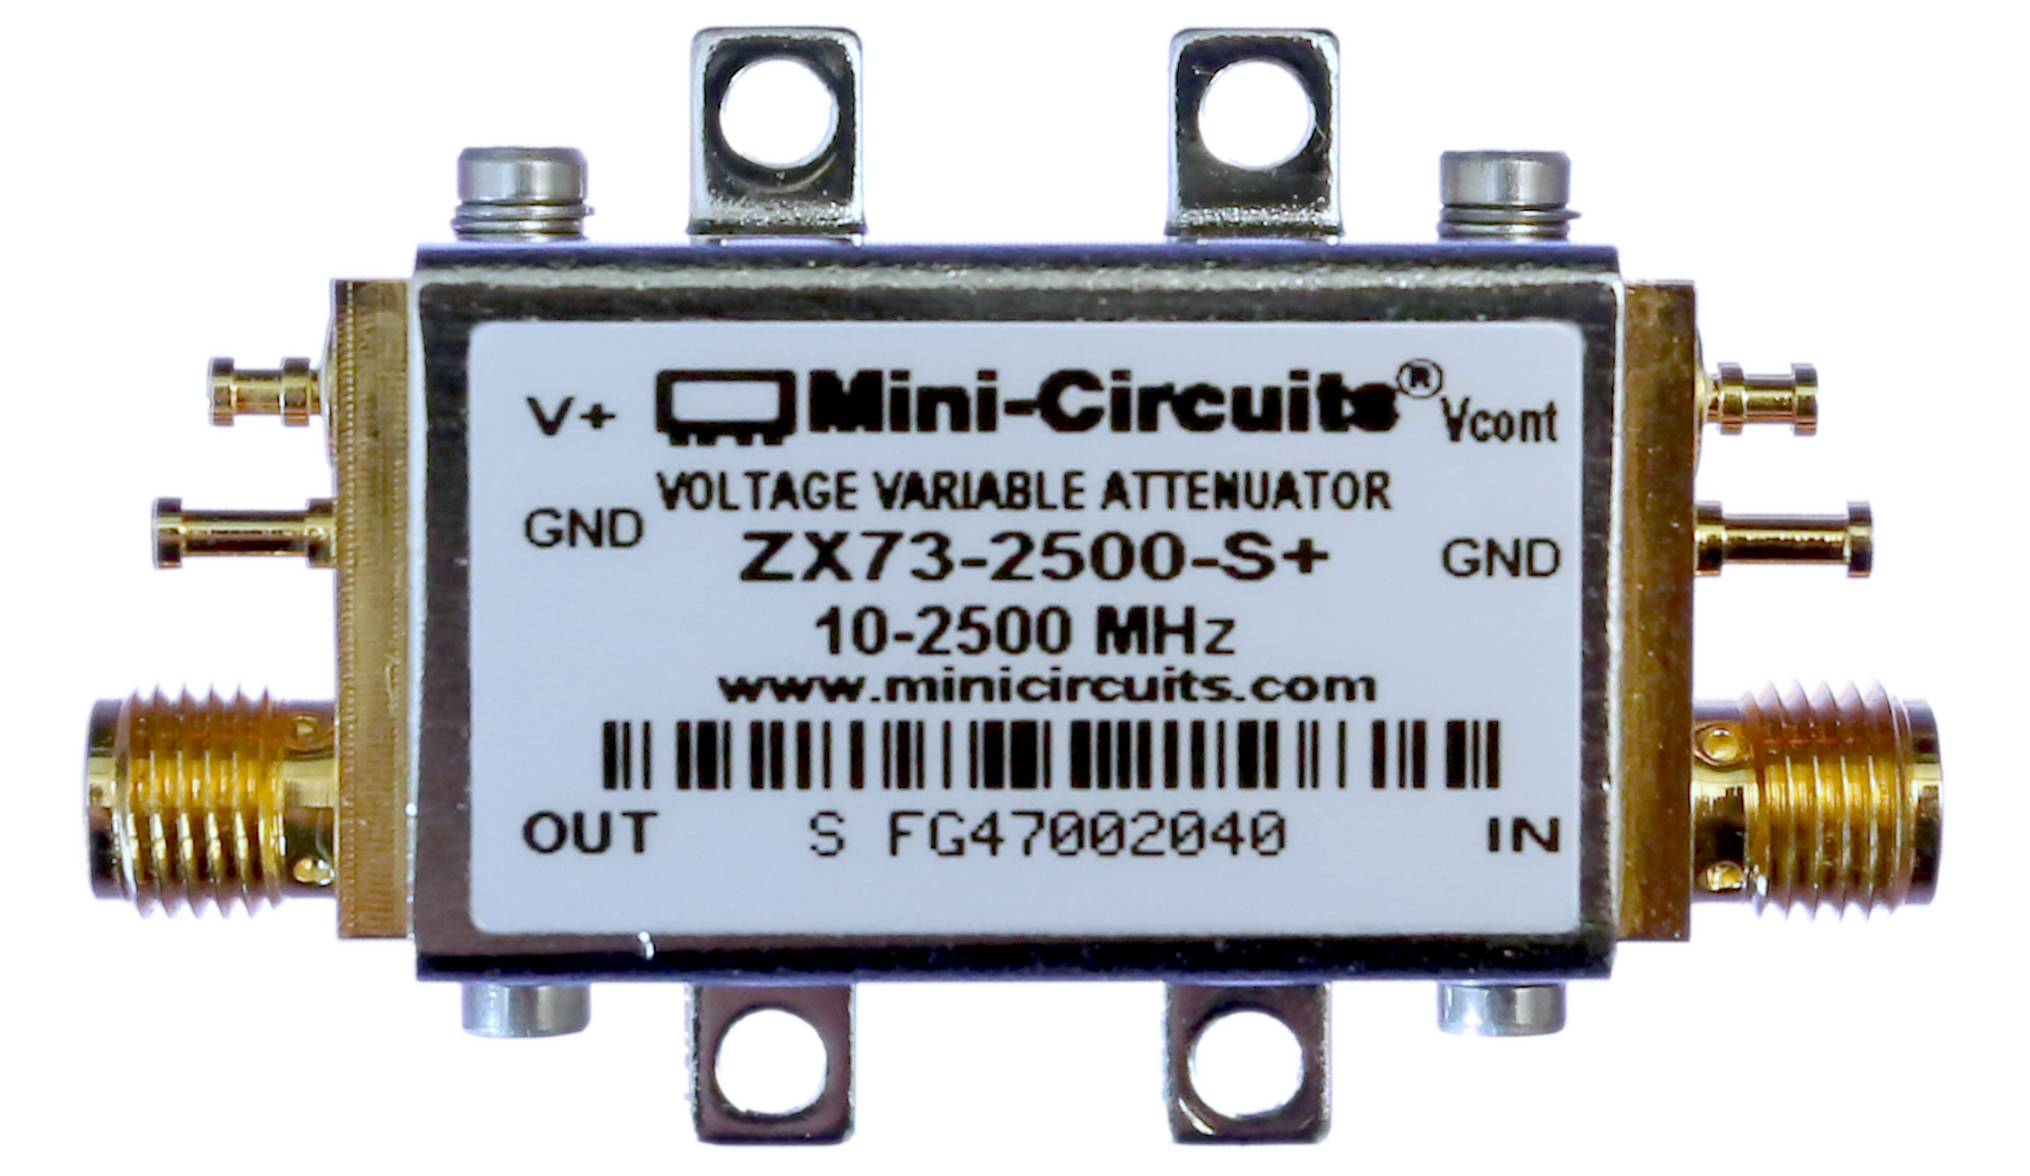
\includegraphics[width=0.3\textwidth]{chap/InterfacingFlute/img/Output/attenuatorOverview/attenClosed}};
\node[] at (2.5,0) {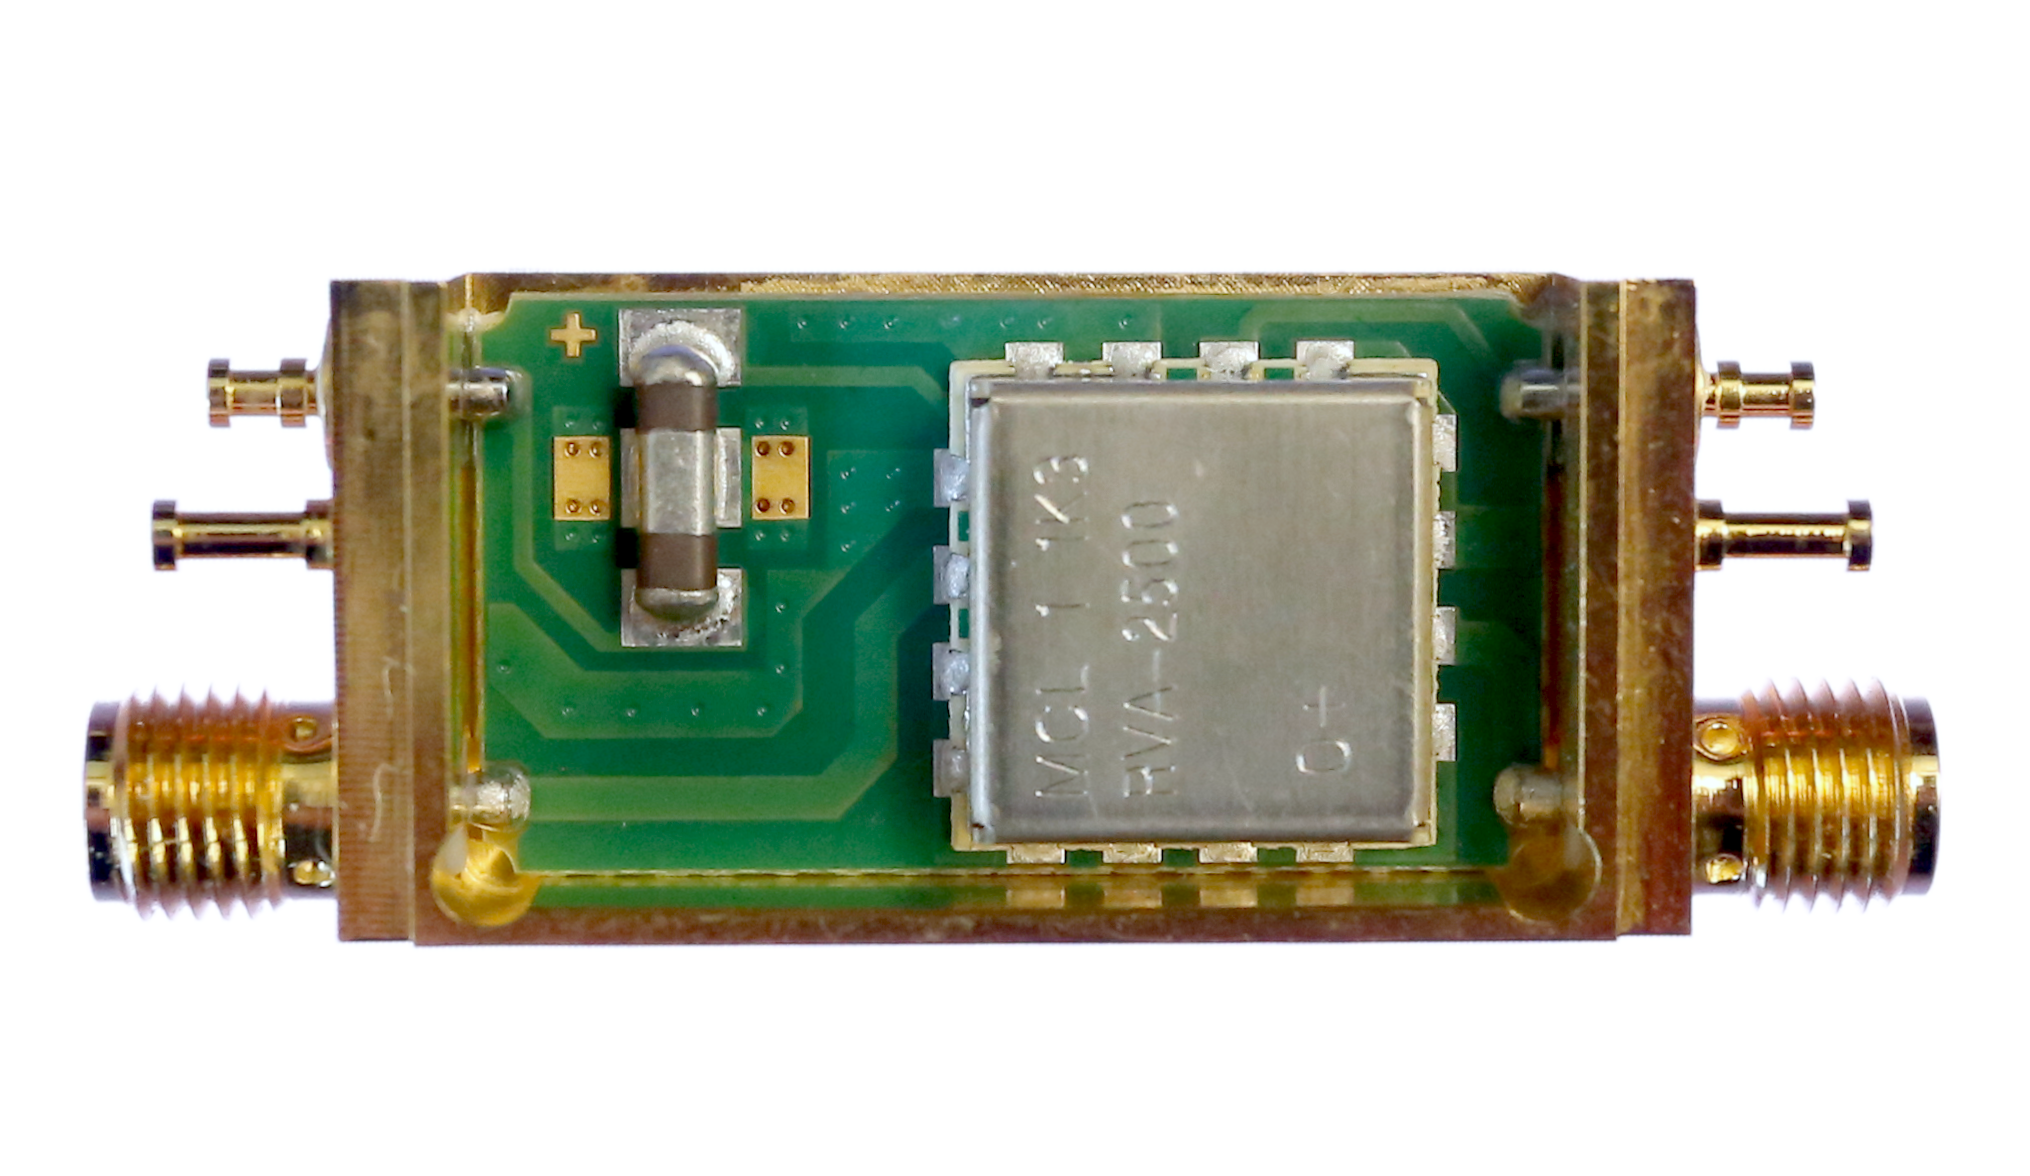
\includegraphics[width=0.3\textwidth]{chap/InterfacingFlute/img/Output/attenuatorOverview/attenOpen}};
\end{tikzpicture}}
		\\
		\subfloat[equivalent circuit from the manufacturer (redrawn from  \cite{mini-circuitsZX732500VoltageVariable})]{\begin{tikzpicture}
\draw (-4.5,0) node[anchor=north,yshift=-0.2cm] {$RF_\text{in}$} to[short, *-] (-2,0) to [full diode,invert] (0,0);
\draw (4.5,0) node[anchor=north,yshift=-0.2cm] {$RF_\text{out}$} to[short, *-] (2,0) to [full diode,invert] (0,0);
\draw (0,2.5) node[anchor=west] {$V_+$} to [short,o-*] ++(0,-1) -- ++(-1.75,0) to [full diode,-*] ++(0,-1.5);
\draw (0,2.5) to [short,o-*] ++(0,-1) -- ++(1.75,0) to [full diode,-*] ++(0,-1.5);
\draw (0,0) to [short,*-o] ++(0,-1) node[anchor=west] {$V_\text{control}$};

\node[fill=white,draw] at (-3,0) {matching};
\node[fill=white,draw] at (3,0) {matching};
\end{tikzpicture}}
		\caption[The controllable attenuator]{The ZX73-2500-S+ controllable \gls{rf} attenuator by Mini-Circuits}
    \label{fig:attenPhotoAndEquiC}
\end{figure}

\begin{figure}[tb]
    \centering
	\begin{tikzpicture}
\draw (0,0) to[full diode] (2,0) to [short] (4,0) to [C=\SI{47}{\nano\farad},-o] (6,0) node[anchor=north,yshift=-0.2cm] {$RF_\text{out}$};
\draw (-6,0) node[anchor=north,yshift=-0.2cm] {$RF_\text{in}$} to [C=\SI{47}{\nano\farad},o-] (-4,0) to [short] (-2,0) to[full diode,invert] (0,0);
\draw (0,3) node[anchor=west] {$V_\text{control}$} to [short,o-] (0,2) to [R=\SI{330}{\ohm},-*] (0,0);
\draw (0,2) to [C=\SI{47}{\nano\farad}] ++(-2,0) node[rground,rotate=-90] {};

\draw (-4,0) to [short,*-] (-4,-2) to [R=\SI{560}{\ohm}] (-4,-4) node[rground] {};
\draw (-2,0) to [full diode,*-] (-2,-2) to [C=\SI{47}{\nano\farad}] (-2,-4) node[rground] {};

\draw (-2,-2) to [R=\SI{1.640}{\kilo\ohm},*-] (0,-2) to [R=\SI{1.640}{\kilo\ohm},-*] (2,-2);
\draw (0,-2) to [R=\SI{680}{\ohm},*-] (0,-4) to [short,-o] (0,-6) node[anchor=west] {$V_\text{control}$};

\draw (4,0) to [short,*-] (4,-2) to [R=\SI{560}{\ohm}] (4,-4) node[rground] {};
\draw (2,0) to [full diode,*-] (2,-2) to [C=\SI{47}{\nano\farad}] (2,-4) node[rground] {};
\end{tikzpicture}

	\caption[Design of a controllable attenuator]{Controllable attenuator design around the HP HSMP-3814 \gls{rf} PIN diodes (redrawn and simplified from \cite{waughLowCostSurfaceMount1992})}
    \label{fig:quadPiequiC}
\end{figure}




The ZX73-2500-S+ attenuator consists of a brass housing/shielding containing the Mini-Circuits RVA-2500+, a variable SMD attenuator in the DV874 case form factor. The \gls{rf} input and output are connected with female SMA screw connectors. The power supply and control voltage are connected with solder pins. In order to use shielded cables and a reliable connection, for all measurements SMA connectors are soldered to the supply and control pins. According to the equivalent circuit in the data sheet \cite{mini-circuitsZX732500VoltageVariable}, it can be assumed it is based on the common quad-$\pi$ pin diode design introduced in \cite{waughLowCostSurfaceMount1992}. In this attenuator design, the resistors in a fixed $\pi$-configuration attenuator are switched out for \gls{rf} PIN diodes with the appropriate biasing and matching resistors and capacitors, see \autoref{fig:quadPiequiC}. At high frequencies, PIN diodes behave like resistors with the differential resistance
\begin{equation}
r_d = f(I_F)
\end{equation}
being an inverse function of the forward bias current, which makes the attenuator adjustable.

The attenuation versus frequency measurements from the manufacturer's data sheet are redone to both get a first impression of the device and verify it is generally operational and also as a sanity check for the used laboratory test equipment.
Because the signal used by the FLUTE \gls{rf} system is a \SI{3}{\GHz} single harmonic, the frequency measurement range is augmented over the maximum of \SI{2.5}{\GHz} in the data sheet to \SI{4}{\GHz}.
Between the measurement of each network analyzer trace, the control voltage $V_\text{control}$ of the attenuator is set to \SI{0}{\volt}, \SI{2}{\volt}, \SI{4}{\volt}, \SI{6}{\volt} or \SI{12}{\volt}.
The result is shown in \autoref{fig:interfacingFlute_atteneval-overview-NA}\footnote{A thru calibration of the network analyzer reduces the influence of the cables and connectors on the measurement. The change in attenuation due to play in the connectors and slight bend changes in the cables exceeds the trace noise (\SI{0.004}{\dB rms}) and causes an uncertainty of about \SI{0.5}{\dB}}.
When comparing the measured plots to the plots in the data sheet, there are obvious discrepancies. For $V_\text{control}=\SI{0}{\volt}$ the attenuator is very susceptible to noise on the control input, which could explain the differences for this curve. In the case of \SI{2}{\volt} and \SI{4}{\volt}, the almost constant offset scales with a similar logarithmic fashion as the attenuation does, which suggests device tolerances causing the deviations.

\begin{figure}[tb]
	\centering
	\includegraphics[width=\textwidth,height=0.5\textwidth]{chap/InterfacingFlute/img/Output/attenuationOverFrequency_Vctrl.tikz}
	\caption[Attenuation vs. frequency plot of the attenuator]{Attenuation vs. frequency over DC control voltage; measured with network analyzer (see section~\ref{app:agilent-e5071c}, parameters: $\#AVG$: 16, $IF\text{-}BW$: \SI{10}{\kHz}); plotted in dashed lines are the measurements from the data sheet (see \cite[p.~2]{mini-circuitsZX732500VoltageVariable})}
	\label{fig:interfacingFlute_atteneval-overview-NA}
\end{figure}

From this quick examination it is not possible to predict how the attenuator behaves for small changes in $V_\text{control}$ and how changes in the environment, such as the body temperature or the supply voltage, cause unwanted variations in the attenuation. 

For this reason, with different measurement setups, the ZX73-2500-S+ is examined in greater detail in the next sections.

To compare desired and spurious influences on the attenuation, the following model is used.\\
The attenuation of the ZX73-2500-S+ $A$ depends on the control voltage $V_\text{control}$ but also on the supply voltage $V+$, the case temperature $\vartheta_\text{case}$ and the \gls{rf} frequency $f$:
\begin{equation}
A=A(\underbrace{V_\text{control},\,V_+,\,\vartheta_\text{case},\,f}_{\vec{x}}) = A\left(\vec{x}\right)
\end{equation}
Other influences are not modeled as they are difficult to control, such as the manufacturing tolerances between different devices, or assumed to be negligible, such as component degradation or humidity.

In the next sections, the influence of each component of the parameter vector $\vec{x}$ on $A$ is measured. As a coarse approximation, all influences are assumed to have linear effect. Then the total derivative of $A$, $\Delta A$ can be written as
\begin{equation}\label{eq:interfacingFlute_linearApprox}
\underbrace{A(\vec{x}-\vec{x_o})-A(\vec{x_o})}_{\Delta A} = \sum_{j=0}^{3} \frac{\Delta A}{\Delta x_j} \Delta x_j
\end{equation}
where the $\nicefrac{\Delta A}{\Delta x_j}$ approximate the partial derivatives $\nicefrac{\d{A}}{\d{x_j}}$.

With \autoref{eq:interfacingFlute_linearApprox}, the maximum error on the attenuation, that is the variation around the operating point with a fixed $V_\text{control}$, can be approximated with
\begin{equation}\label{eq:interfacingFlute_maxerror}
\Delta A_{\text{max}} = \sum_{j=0}^{3} \left|\frac{\Delta A}{\Delta x_j} \cdot \Delta x_j\right| 
= \sum_{j=0}^{3} \left|\frac{\Delta A}{\Delta x_j}\right| \cdot \left|\Delta x_j\right|.
\end{equation}

If not specified otherwise, the operating point
\begin{align}\label{eq:interfacingFlute_operatingpoint}
A(\vec{x_o}) =: A_o &= A(V_\text{control},\,V_+,\,\vartheta_\text{case},\,f)\\
A_o                 &= A\left(\SI{10}{\volt},\,\SI{3}{\volt},\,\SI{20}{\celsius},\,\SI{3}{\GHz}\right)
\end{align}
is used.

\subsubsection{Common Measurement Setup}
For the following measurements a common setup is used to ease the recording of data and the sequential control for parameter studies. The needed tasks are:
\begin{itemize}
\item Supply the attenuator with the supply voltage $V_+$
\item Supply the attenuator with the adjustable control voltage $V_\text{control}$
\item Supply the \gls{rf} input power with variable frequency $f$
\item Measure the \gls{rf} output power
\item Record all data as time series to a computers storage device
\end{itemize}

To achieve this, the setup in \autoref{fig:interfacingFlute_atteneval-setup} is used.
The supply and control voltage are generated by a Keysight 34972A with a 34907A module (see section~\ref{app:keysight-34972A}).
To get a more accurate measurement of the actual voltages, two digital multimeters (Models 34470A and 34411A, see section~\ref{app:keysight-34470A}) are connected directly at the $V_\text{control}$ and $V_+$ pins.
The \gls{rf} signal is generated by a Rhode und Schwarz SMC 100A signal generator (see section~\ref{app:smc}).
With the HP E4419B (see section~\ref{app:hpe4419}) and its two inputs and a power splitter, it is possible to directly get the attenuation of the ZX73-2500-S+.
The body temperature of the device is monitored with a PT100 temperature sensor connected to the 34972A.

Each of the lab devices used is compatible with \gls{vxi-11}, which is a widely adopted standard that is used to send \gls{ascii} \gls{scpi} commands over an ethernet network (called \gls{lxi}) or \gls{gpib}.\cite{lxi2021}
This enables remote and programatically control of the devices over the network.
With the library \textit{python-vxi11}, it is now possible to write a custom script, that sets the measurement devices to known initial conditions, drives the inputs of the attenuator and records the generated data. Timing the output of new set-values and recording of data is done with the \textit{Advanced Python Scheduler}.\cite{apscheduler}\\ 
The whole setup of the hardware in \autoref{fig:interfacingFlute_atteneval-setup} and the Python software, a measurement frequency of about \SI{0.5}{\Hz} to \SI{1}{\Hz} can be achieved, which is enough because most measurements taken are of a static nature and in the case of the temperature influence measurement, the thermal time constant is in the order of a few seconds.
The limiting device is the HP E4419B which takes the longest to perform one measurement. Without it, measurement frequencies of over \SI{4}{\Hz} are possible.

All measurements are performed in the ``\gls{rf} lab'' in building 348 (\gls{kara} hall on KIT Campus North) which is air conditioned to about \SI{20(2)}{\celsius}.

\begin{figure}[tb]
	\centering
	\includegraphics[]{chap/InterfacingFlute/img/Output/schematic.tikz}
	\caption[Measurement setup to evaluate the attenuator]{Measurement setup: DUT(red), \gls{rf} generator/power splitter/meter(blue),\\ DC sources/meters(green), temperature probe(yellow)}
	\label{fig:interfacingFlute_atteneval-setup}
\end{figure}

\subsubsection{Relation between Control Voltage and Attenuation}
In this section, the relation between the control voltage and the attenuation is examined. All other parameters are kept constant:
\begin{equation}
A(\vec{x}) := A(V_\text{control})
\end{equation}

The measured spectra in \autoref{fig:interfacingFlute_atteneval-overview-NA} already suggest that there is a non linear relationship between the control voltage $V_\text{control}$ and the attenuation $A(V_\text{control})$ of the attenuator:
\begin{equation}
A(V_\text{control}) \neq const. \cdot V_\text{control} + A_0.
\end{equation}
This also means the sensitivity
\begin{equation}
S(V_\text{control}) := \frac{\Delta A(V_\text{control})}{\Delta V_\text{control}}
\end{equation}
is not a constant.
In other words, for a desired relative change in attenuation, the needed adjustment in $V_\text{control}$ depends on the chosen operating point $A_o=A(V_\text{control,o})$.

With all other variables being at the operating point in \autoref{eq:interfacingFlute_operatingpoint}, $A(V_\text{control})$ is measured by stepping $V_\text{control}$ in \SI{0.1}{\volt} increments up and down between \SI{0}{\volt} and \SI{12}{\volt} several times with each valued held constant for \SI{30}{\second}. $A(V_\text{control})$ is then calculated as the mean of all measurements $A_j(V_\text{control})$ with the same $V_\text{control}$ with

\begin{equation}\label{eq:interfacingFlute_avg}
A(V_\text{control}) = \frac{1}{N} \sum_{j=0}^{N-1} A_j(V_\text{control}).
\end{equation}

With the averaging done in \autoref{eq:interfacingFlute_avg} and $N=120$, the resulting mean standard deviation is $\sigma_A=\SI{0.00574}{\dB}$.
\autoref{fig:interfacingFlute_attenDatten} shows the resulting plot.

The plot shows the attenuation can be varied over more than \SI{30}{\dB} and the magnitude of the sensitivity being large for small control voltages (\SIrange{1}{3}{\volt}).
Since the required change in attenuation of less than \SI{1}{\dB} is much smaller, it is only necessary to vary $V_\text{control}$ around the operating point.

The optimal operating point for $V_\text{control}$ is selected by considering the following three aspects.
First, the absolute attenuation at the operating point should be as low as possible to not worsen the \gls{snr} of the signal path. Second the control voltage has to fit in the possible output voltage range of the voltage source and still allow for adjustment towards both lower and higher voltages. 
In case of the Keysight 34972A/34907A the maximum possible output voltage is \SI{12}{\volt}.
Third, the sensitivity should be as low as feasible to make the attenuation less susceptible to noise on the $V_\text{control}$ input.


For these reasons, $V_\text{control,o}=\SI{10}{\volt}$ (as already used in \autoref{eq:interfacingFlute_operatingpoint}) is chosen as the operating point, which allows $V_\text{control}$ to be varied in \SIrange{8}{12}{\volt}.
At the operating point $\vec{x_o}$ (with $V_\text{control,o}=\SI{10}{\volt}$), the measured attenuation is
\begin{equation}
A(V_\text{control})=\SI{6.4859}{\dB}
\end{equation}
\autoref{fig:interfacingFlute_attenDattenZoomed} shows the attenuation and sensitivity around the operating point.

The sensitivity at the operating point is determined with discrete forward differentiation as
\begin{equation}
S(V_\text{control})=S(\SI{10}{\volt})=\frac{\Delta A}{\Delta V_\text{control}} = \SI{-0.151}{\dB\per\volt}.
\end{equation}

For further error calculations, the maximum $\nicefrac{\Delta A(V_\text{control})}{\Delta V_\text{control}}$ is needed. \autoref{fig:interfacingFlute_attenDattenZoomed} shows the maximum magnitude of $\nicefrac{\Delta A(V_\text{control})}{\Delta V_\text{control}}$ to be at the lower edge of the $V_\text{control}$ range of $S(\SI{8}{\volt})$:
\begin{equation}
\left[\frac{\Delta A(V_\text{control})}{\Delta V_\text{control}}\right]_{\text{max}}=\SI{-0.242}{\dB\per\volt}
\end{equation}

The minimum possible step size of the attenuation can be calculated using $\left[\nicefrac{\Delta A(V_\text{control})}{\Delta V_\text{control}}\right]_{\text{max}}$ and the DAC output resolution of the Keysight 34907A ($\nicefrac{\SI{24}{\volt}}{2^{16}-1}=\SI{366.22}{\micro\volt}$):
\begin{equation}
\delta A(V_\text{control}) = \SI{0.242}{\dB\per\volt} \cdot \SI{366.22}{\micro\volt} = \SI{0.00008862524}{\dB}
\end{equation}

To assess the stability of $V_\text{control}$, delivered from the Keysight 34972A (see \autoref{app:keysight-34972A}) \gls{dac}, its stability over the course of one day is measured. For that the voltage is taken once every 2 seconds with a Keysight 34470A multimeter (see \autoref{app:keysight-34470A}). The result is shown in \autoref{fig:interfacingFlute_vcontrolstab_longterm}.

This measurement shows the stability of $V_\text{control}$ to be
\begin{equation}
\sigma_{V_\text{control}} = \SI{0.173}{\milli\volt}
\end{equation}

\begin{figure}[H]
	\centering
	\includegraphics[width=\textwidth,height=0.65\textwidth]{chap/InterfacingFlute/img/Output/attenAndDattten.tikz}
	\caption[Attenuation vs control voltage]{Measured attenuation $A(V_\text{control},f=\SI{3}{\GHz})$ of the ZX73-2500-S+ as a function of the control voltage input $V_\text{control}$ along with the sensitivity $S(V_\text{control},f=\SI{3}{\GHz})$}
	\label{fig:interfacingFlute_attenDatten}
\end{figure}

\begin{figure}[H]
	\centering
	\includegraphics[width=\textwidth,height=0.65\textwidth]{chap/InterfacingFlute/img/Output/attenAndDatttenZoomed.tikz}
	\caption[Detailed version of \autoref{fig:interfacingFlute_attenDatten}]{Zoomed in version of \autoref{fig:interfacingFlute_attenDatten} shows the attenuation and sensitivity around the operating point $V_\text{control,o}=\SI{10}{\volt}$}
	\label{fig:interfacingFlute_attenDattenZoomed}
\end{figure}

\begin{figure}[H]
	\centering
	\includegraphics[width=\textwidth,height=0.5\textwidth]{chap/InterfacingFlute/img/Output/Vcontrolstab.tikz}
	\caption[Long term stability of the control voltage]{Long term stability of $V_\text{control}$ as delivered by the Keysight 34972A DAC (ch. 205); measured with Keysight 34470A;\\room temperature during measurement: $\mu_\vartheta=\SI{19.12}{\degreeCelsius}$, $\sigma_\vartheta=\SI{0.28}{\degreeCelsius}$}
	\label{fig:interfacingFlute_vcontrolstab_longterm}
\end{figure}

\subsubsection{Influence of Supply Voltage Noise on Attenuation}
To get the required stability for the power supply voltage, the effect of the supply voltage $V_+$ on the attenuation $\nicefrac{\Delta A}{\Delta V_+} (V_+)$ has to be examined first. To do that $V+$ is varied \SI{\pm0.2}{\volt} around the nominal supply voltage at the operating point $V_{+_o}=\SI{3}{\volt}$, all other parameters are kept constant and the attenuation is measured. To make the measurement more robust against fluctuations of the room temperature and drift of the devices, the procedure of stepping through the voltages is repeated in a similar fashion as for the influence of $V_\text{control}$ and the means for each set $V_+$ are computed. The result is shown in \autoref{fig:interfacingFlute_atteneval-vsupp-influence}.

The plot shows $A(V_+)$ to be of linear nature over the measured range.
Therefore using a linear regression of the measured data points, the influence on the attenuation can be estimated to
\begin{equation}
\frac{\Delta A(V_+)}{\Delta V_+}(V_+) 
\approx \frac{\Delta A(V_+)}{V_+} 
= \left[\frac{\Delta A(V_+)}{V_+}\right]_\text{max}
=\SI{0.0035592}{\dB\per\volt}.
\end{equation}

Next the stability of the supply voltage is measured.
for that the stability over the course of one day is measured. The voltage is taken once every two seconds with a Keysight 34470A multimeter (see \autoref{app:keysight-34470A}). The result is shown in \autoref{fig:interfacingFlute_atteneval-vsupp-stability}.


Comparing \autoref{fig:interfacingFlute_atteneval-vsupp-stability} with \autoref{fig:interfacingFlute_vcontrolstab_longterm} suggests a relation between the deviations in $V_\text{control}$ and $V_+$. Since they are both generated by the same Keysight 34907A module, this is plausible. The slightly changing room temperature is assumed to be the common cause.
By calculating the correlation coefficients between $\Delta V_+$ and $\Delta V_\text{control}$ and also between $\Delta V_+$ and $\Delta \vartheta_\text{ambient}$, this can be verified:
\begin{align}
\text{Corr}(\Delta V_+,\Delta V_\text{control})         &= \num{0.99204} \\
\text{Corr}(\Delta V_+,\Delta \vartheta_\text{ambient}) &= \num{-0.92242} \\
\end{align}

The long term measurement yields a standard deviation of
\begin{equation}
\sigma_{V,+,\text{longterm}} = \SI{0.154}{\milli\volt},
\end{equation}
which is also used as the worst case stability
\begin{equation}
\sigma_{V_+} = \SI{0.154}{\milli\volt}
\end{equation}

There is also a constant offset of $\mu_{V,+,\text{longterm}}=\SI{-1.35}{\milli\volt}$, but it is disregarded since it can easily be compensated by slightly increasing the supply voltage.

\begin{figure}[H]
	\centering
	\includegraphics[width=\textwidth,height=0.5\textwidth]{chap/InterfacingFlute/img/Output/VsuppStab/influenceVplus.tikz}
	\caption{Influence of the supply voltage $V_+$ on the attenuation}
	\label{fig:interfacingFlute_atteneval-vsupp-influence}
\end{figure}

\begin{figure}[H]
	\centering
	\includegraphics[width=\textwidth,height=0.5\textwidth]{chap/InterfacingFlute/img/Output/VsuppStab/stabilityVplus.tikz}
	\caption[Long term stability of the supply voltage]{Long term stability of $V_{+}$ as delivered by the Keysight 34972A DAC (ch. 204); measured with Keysight 34470A;\\room temperature during measurement: $\mu_\vartheta=\SI{19.12}{\degreeCelsius}$, $\sigma_\vartheta=\SI{0.28}{\degreeCelsius}$}
	\label{fig:interfacingFlute_atteneval-vsupp-stability}
\end{figure}

\newpage
\subsubsection{Influence of RF Frequency on Attenuation}
In this section the influence of a varying \gls{rf} frequency on attenuation $\nicefrac{\Delta A}{\Delta f} (f)$ is examined. For that the set frequency of the R\&S SMC100 signal generator is varied while the attenuation is measured. The result is shown in \autoref{fig:interfacingFlute_atteneval-rf}.

\begin{figure}[H]
    \centering
        \subfloat[$f=f_o \SI{+-30}{\kHz}$]{% This file was created by tikzplotlib v0.9.5.
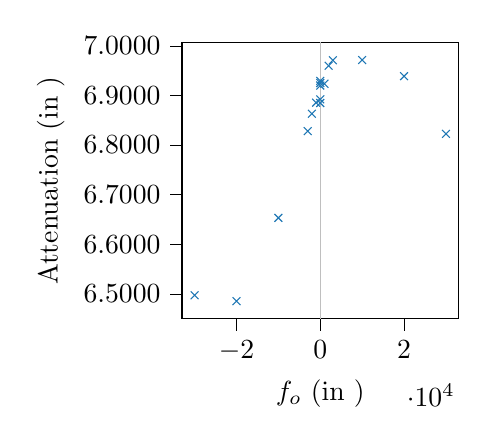
\begin{tikzpicture}[
baseline,
]

\definecolor{color0}{rgb}{0.12156862745098,0.466666666666667,0.705882352941177}

\begin{axis}[
height=0.42\textwidth,
ytick distance=0.1,
tick align=outside,
tick pos=left,
width=0.42\textwidth,
x grid style={white!69.0196078431373!black},
xlabel={$f_o$ (in \si{\kHz})},
xmin=-33000.0073466986, xmax=33000.0073466986,
xtick style={color=black},
y grid style={white!69.0196078431373!black},
ylabel style={align=center},
ylabel={Attenuation (in \si{\dB})},
ymin=6.44956234557695, ymax=7.00689920227556,
ytick style={color=black},
yticklabel pos=lower,
y tick label style={
        /pgf/number format/.cd,
            fixed,
            fixed zerofill,
            precision=4,
        /tikz/.cd
    }
]
\draw[gray!50] ({axis cs:0,0}|-{rel axis cs:0,1}) -- ({axis cs:0,0}|-{rel axis cs:0,0});
\addplot [only marks, mark=x, draw=color0]
table{%
x                      y
-29999.9999999998 6.49704080362745
-20000 6.48517944823129
-9999.99999999979 6.65312661396739
-3000.00000000011 6.82805338711268
-1999.99999999978 6.86303896803419
-999.99999999989 6.88534599751244
-1.00000000013978 6.91995292566434
0 6.89215273989011
0 6.88470073226562
0 6.92509045190909
1.00000000013978 6.92927676035294
999.99999999989 6.92353152521008
1999.99999999978 6.95979922043103
3000.00000000011 6.97091072853147
9999.99999999979 6.97128209962121
20000 6.93879379212121
29999.9999999998 6.82251071210526
};
\end{axis}

\end{tikzpicture}
}
        \qquad
        \subfloat[$f=f_o \SI{+-1}{\kHz}$]{% This file was created by tikzplotlib v0.9.5.
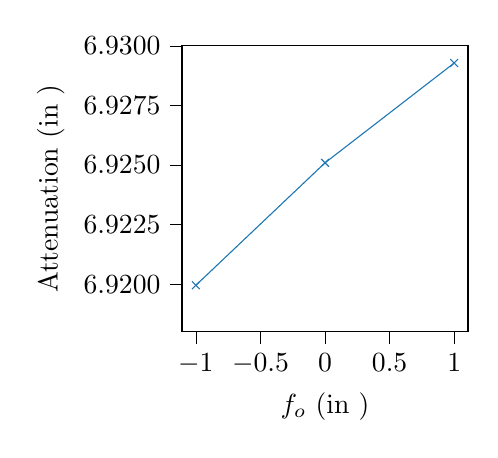
\begin{tikzpicture}[
baseline
]

\definecolor{color0}{rgb}{0.12156862745098,0.466666666666667,0.705882352941177}

\begin{axis}[
height=0.43\textwidth,
ytick distance=0.0025,
tick align=outside,
tick pos=left,
width=0.43\textwidth,
x grid style={white!69.0196078431373!black},
xlabel={$f_o$ (in \si{\kHz})},
xmin=-1.10734669900456, xmax=1.10734669900456,
xtick style={color=black},
y grid style={white!69.0196078431373!black},
ylabel style={align=center},
ylabel={Attenuation (in \si{\dB})},
ymin=6.918, ymax=6.93,
ytick style={color=black},
yticklabel pos=lower,
y tick label style={
        /pgf/number format/.cd,
            fixed,
            fixed zerofill,
            precision=4,
        /tikz/.cd
    }
]
\addplot [mark=x, draw=color0,]
table{%
x                      y
-1.00000000013978 6.91995292566434
0 6.92509045190909
1.00000000013978 6.92927676035294
};
\end{axis}

\end{tikzpicture}
}
       \caption[Influence of an offset frequency on attenuation]{Influence of an offset frequency $f-\SI{3}{\GHz}$ on the attenuation }
    \label{fig:interfacingFlute_atteneval-rf}
\end{figure}

Phase noise measurements of the \gls{flute} main oscillator\footnote{Using the phase noise analyzer HA7062C by Holzworth, see section~\ref{app:holzworth-ha7062c}} yield the phase noises
\begin{align}
\mathscr{L}(f_o=\SI{10}{\hertz}) &= \SI{-78.63}{\dB c}\\
\mathscr{L}(f_o=\SI{1}{\kilo\hertz}) &= \SI{-116.26}{\dB c}\\
\mathscr{L}(f_o=\SI{10}{\kilo\hertz}) &= \SI{-139.29}{\dB c}\\
\mathscr{L}(f_o=\SI{1}{\mega\hertz}) &= \SI{-142.29}{\dB c},
\end{align}

with $f_o$ being the offset frequency from the carrier and the unit \si{\dB c} measuring the offset power from the carrier.

Since this shows the oscillator to be much more stable than $f_o=\SI{10}{\kHz}$, is it is sufficient to consider only \autoref{fig:interfacingFlute_atteneval-rf} (b). In the range of \SI{\pm1}{\kHz} around the operating point frequency of \SI{3}{\GHz}, $\nicefrac{\Delta A}{\Delta f} (f)$ is almost constant. From the data points, the value can be calculated to
\begin{equation}
\frac{\Delta A(f)}{\Delta f}(f) 
\approx \frac{\Delta A(f)}{\Delta f} 
= \left[\frac{\Delta A(f)}{\Delta f}\right]_\text{max}
=\SI{0.0000046619}{\dB\per\hertz}.
\end{equation}

\subsubsection{Influence of Case Temperature Variations on Attenuation}
To get insight into the importance of a stable case temperature, its influence on the attenuation $\nicefrac{\Delta A}{\Delta \vartheta_\text{case}} (\vartheta_\text{case})$ and the temperature stability both in the ``\gls{rf} lab'' and the final mounting position inside the FLUTE \gls{llrf} cabinet are measured.

To measure $\nicefrac{\Delta A}{\Delta \vartheta_\text{case}} (\vartheta_\text{case})$, the following experimental setup is used.\\
The bottom of the attenuator is fixed to a rectangular iron profile with zip ties. Then the iron profile is heated with the tip of a soldering iron (set to \SI{150}{\degreeCelsius}) for \SI{1}{\minute} and then allowed to cool for \SI{20}{\minute}. This cycle is repeated three times and the device temperature and the attenuation are measured once every \SI{2}{\second}. Due to heat flowing from the soldering iron to the iron profile and through device itself, a strong hysteresis between the heating and cooling cycle can be observed in \autoref{fig:interfacingFlute_atteneval-tempstab-influence}.

\begin{figure}[tb]
	\centering
	\includegraphics[width=\textwidth,height=0.5\textwidth]{chap/InterfacingFlute/img/Output/temperature/influenceTemp.tikz}
	\caption[Influence of the case temperature on attenuation]{Raw measurement result of the influence of the case temperature $\vartheta_\text{case}$ on the attenuation; color coded is the relative elapsed time of the measurement}
	\label{fig:interfacingFlute_atteneval-tempstab-influence}
\end{figure}

To get $\nicefrac{\Delta A}{\Delta \vartheta_\text{case}} (\vartheta_\text{case})$ from the plot in \autoref{fig:interfacingFlute_atteneval-tempstab-influence}, an approximately linear relationship $A(\vartheta_\text{case})$ is assumed. To get the slope, the $\vartheta_\text{case}$ component of the measured data points $(\vartheta_\text{case}|A(\vartheta_\text{case}))$ are rounded to one decimal place. Then, data points with the same $A(\vartheta_\text{case})$ are averaged together and a linear regression is applied to the result. See \autoref{fig:interfacingFlute_atteneval-tempstab-influenceMean} for the resulting plot. The linear regression estimator yields
\begin{equation}
\frac{\Delta A}{\Delta \vartheta_\text{case}} (\vartheta_\text{case})
\approx \frac{\Delta A}{\Delta \vartheta_\text{case}}
= \left[\frac{\Delta A}{\Delta \vartheta_\text{case}}\right]_\text{max}
= \SI{0.00432449}{\dB\per\celsius}.
\end{equation}

Next, the temperature stability in both the ``\gls{rf} lab'' and in the FLUTE \gls{llrf} cabinet is measured. For that in each environment the temperature is recorded over night with a thermo element connected to the Keysight 34907A inside the Keysight 34972A every two seconds.

From the data in \autoref{fig:interfacingFlute_atteneval-tempstab-time}, the corresponding stabilities are calculated to be
\begin{align}
\sigma_{\vartheta_\text{ambient, RF lab}}       &= \SI{0.1067}{\celsius}\\
\sigma_{\vartheta_\text{ambient, LLRF cabinet}} &= \SI{0.0288}{\celsius}.
\end{align}
This assumes the case of the attenuator and the ambient around it being in thermal equilibrium. With the thick brass case and its only weakly mechanically mounting to the metal support, the attenuator posses a significant thermal time constant $\tau_{th}=R_\text{th}C_\text{th}$. Therefore, thermally the attenuator is a lowpass filter and cannot follow fast changes in the ambient temperature.
This means only slow changes of the ambient temperature have an influence on $A$, so short changes, like opening a door, have only a minor effect.

\begin{figure}[H]
	\centering
	\includegraphics[width=\textwidth,height=0.5\textwidth]{chap/InterfacingFlute/img/Output/temperature/influenceTempmean.tikz}
	\caption[Processed data from \autoref{fig:interfacingFlute_atteneval-tempstab-influence}]{Influence of the case temperature $\vartheta_\text{case}$ on the attenuation}
	\label{fig:interfacingFlute_atteneval-tempstab-influenceMean}
\end{figure}

\begin{figure}[H]
	\centering
	\includegraphics[width=\textwidth,height=0.65\textwidth]{chap/InterfacingFlute/img/Output/temperature/tempStability.tikz}
	\caption[Measured temperature stability]{Comparison between the temperature stability in the ``\gls{rf} lab'' and inside the FLUTE \gls{llrf} cabinet}
	\label{fig:interfacingFlute_atteneval-tempstab-time}
\end{figure}

\newpage
\subsubsection{$V_\text{control}$ Frequency response}\label{sec:interfacingFlute_freqr}
Using a non inverting adder with a TS912IN operational amplifier, a sine wave with constant offset is created, which is then used to drive the control voltage $V_\text{control}$. The results for different sine wave frequencies are shown in \autoref{fig:interfacingFlute_atteneval-freqresp}.

This result is to be interpreted purely qualitatively, as neither measurement device and software is designed for this kind of measurement, nor is the circuit used optimal in the sense of the bandwidth and high input impedances.
But the traces in \autoref{fig:interfacingFlute_atteneval-freqresp} verify that the ZX73-2500-S+ attenuator is able to follow changes of $V_\text{control}$ at least up to a few ten \si{\kHz}. If the attenuator should be set to a new value, this is equivalent to applying a step at the attenuators $V_\text{control}$ input which, according to the Fourier transform of a $\text{rect}(t)$ pulse, a $\text{sinc}(f)$, contains high frequencies.

This is several orders of magnitude larger than the control system can input, compute and output new values to the attenuator.

\begin{figure}[H]
	\centering
	\includegraphics[width=\textwidth,height=0.6\textwidth]{chap/InterfacingFlute/img/Output/holzworth.tikz}
	\caption[Spectrum showing maximum modulation speed]{Spectrum (measured with Holzworth HA7062A (see section~\ref{app:holzworth-ha7062c})) showing the effect of modulating $V_\text{control}$ with different frequencies (Modulation amplitude: \SI{1}{\volt})}
	\label{fig:interfacingFlute_atteneval-freqresp}
\end{figure}

\newpage
\subsection{Combined Maximum Error and Conclusion}
Using \autoref{eq:interfacingFlute_maxerror} and setting $\Delta x_j = \sigma_{x_j}$ and $\nicefrac{\Delta A}{\Delta x_j} = \left[\nicefrac{\Delta A}{\Delta x_j}\right]_\text{max}$, the upper bound on the deviation of the attenuation, that is the error $\Delta A$ in the worst case, can now be calculated:
\begin{align}
\Delta A_{\text{max}} &= \sum_{j=0}^{3} \left|\frac{\Delta A}{\Delta x_j} \cdot \Delta x_j\right|\\
                      &= \left|\frac{\Delta A}{\Delta V_\text{control}} \cdot \Delta V_\text{control}\right|
                      +  \left|\frac{\Delta A}{\Delta V_{+}} \cdot \Delta V_{+}\right|
                      +  \left|\frac{\Delta A}{\Delta f} \cdot \Delta f\right|
                      +  \left|\frac{\Delta A}{\Delta \vartheta_\text{case}} \cdot \Delta \vartheta_\text{case}\right|\\
                      &=       \underbrace{\SI{0.242}{\dB\per\volt} \cdot \SI{0.173}{\milli\volt}}_{\SI{41.9}{\micro\dB\relax}}\\
                      &\quad+  \underbrace{\SI{0.0035592}{\dB\per\volt} \cdot \SI{0.154}{\milli\volt}}_{\SI{548}{\nano\dB\relax}}\\
                      &\quad+  \underbrace{\SI{0.00000466}{\dB\per\hertz} \cdot \SI{0}{\hertz}}_{\SI{0}{\dB\relax}}\\
                      &\quad+  \underbrace{\SI{0.004325}{\dB\per\celsius} \cdot \SI{0.11}{\celsius}}_{\SI{475.75}{\micro\dB\relax}}\\
                      &= \SI{518}{\micro\dB\relax} = \SI{0.000518}{\dB}
\end{align}

This shows that even in the worst case, the set attenuation of the ZX73-2500-S+ attenuator is stable within the requirement.

The other requirements from \autoref{tab:interfacingFlute_rfattenrequirements} are also fulfilled, see \autoref{tab:interfacingFlute_rfattenrequirements_result}.

\begin{table}[tbh]
\caption[Evaluation results]{ZX73-2500-S+ controllable \gls{rf} attenuator evaluation test results}
\label{tab:interfacingFlute_rfattenrequirements_result}
\centering
\begin{tabular}{lccl}
	\toprule
	Requirement                            &      {Value/Range} set      &  {Value/Range} actual   & Verdict \\ \midrule
	attenuation adjustment                 &    $\ge\SI{\pm0.2}{\dB}$    &    \SI{\pm0.3}{\dB}     & pass    \\
	attenuation stability                  &   $\le\SI{\pm0.001}{\dB}$   &   \SI{0.000518}{\dB}    & pass    \\
	nominal attenuation at operating point &      $\le\SI{10}{\dB}$      &      \SI{6.6}{\dB}      & pass    \\
	attenuation resolution                 &    $\le\SI{0.001}{\dB}$     &   \SI{0.000089}{\dB}    & pass    \\
	setup time                             & $\le\SI{10}{\milli\second}$ &       \SI{1}{\ms}       & pass    \\
	operating temperature range            &   \SI{25\pm0.1}{\celsius}   & \SI{25\pm0.1}{\celsius} & pass    \\
	supply voltage                         &   \SIrange{3}{12}{\volt}    &      \SI{3}{\volt}      & pass    \\
	control voltage                        &   \SIrange{3}{12}{\volt}    & \SIrange{8}{12}{\volt}  & pass    \\ \bottomrule
\end{tabular}
\end{table}

\subsection{Test of the Attenuator with FLUTE}
In this section the attenuator in mounted at \gls{flute} and its function is verified against the data gathered in the lab in earlier sections.

The attenuator is installed at its final mounting location inside the \gls{llrf} cabinet in the \gls{flute} bunker basement and is connected between the output of the vector modulator (after the oscillator, not shown in \autoref{fig:fluteEgun-rfschematic}) and the input of the pre-amplifier. With the controllable attenuator at its operating point, the signal path now contains an attenuation of about \SI{6}{\dB} at all times.

After all components of \gls{flute} are warmed up to operational temperatures, the attenuation versus control voltage curve $A(V_\text{control})$ is measured again (compare the lab measurement \autoref{fig:interfacingFlute_attenDatten}).

To do so, the control voltage $V_\text{control}$ is varied in \SI{0.5}{\volt} steps (see \autoref{fig:interfacingFlute_finalTest_calv}), with each step kept for \SI{20}{\minute}. Synchronous to that, the \gls{rf} power of the cavity is recorded (see \autoref{fig:interfacingFlute_finalTest_calp}), from which the attenuation $A$ can be calculated. Computing the averaging over each step yields $A(V_\text{control})$. It is depicted in \autoref{fig:interfacingFlute_finalTest} together with its uncertainty.


\begin{figure}[tbh]
	\centering
	\includegraphics[width=\textwidth,height=0.3\textwidth]{chap/InterfacingFlute/img/Output/cal/cal_V.tikz}
	\caption[Evaluation control voltage signal]{Time signal $V_\text{control}$ used to calculate \autoref{fig:interfacingFlute_finalTest}}
	\label{fig:interfacingFlute_finalTest_calv}
\end{figure}

\begin{figure}[tbh]
	\centering
	\includegraphics[width=\textwidth,height=0.3\textwidth]{chap/InterfacingFlute/img/Output/cal/cal_P.tikz}
	\caption[Evaluation measured attenuation]{Time signal $A(V_\text{control})$ used to calculate \autoref{fig:interfacingFlute_finalTest}}
	\label{fig:interfacingFlute_finalTest_calp}
\end{figure}

\begin{figure}[tbh]
	\centering
	\includegraphics[width=\textwidth,height=0.4\textwidth]{chap/InterfacingFlute/img/Output/attenFluteErrorbars.tikz}
	\caption[Evaluation attenuation vs control voltage]{Measured $A(V_\text{control})$ with \gls{flute}; error bars show the span between minimum and maximum values in each $V_\text{control}$ step}
	\label{fig:interfacingFlute_finalTest}
\end{figure}



